\pdfinfoomitdate=1
\pdftrailerid{}
\pdfsuppressptexinfo=-1
\documentclass[10pt,a4paper]{article}
\usepackage{cmap}
\usepackage[margin=1.8cm,headheight=14pt,headsep=10pt]{geometry}
\usepackage[leqno]{amsmath}
\usepackage{amssymb,booktabs,longtable,array,ragged2e,multicol,multirow,xcolor,fancyhdr,tikz}
\definecolor{linkblue}{rgb}{0.08,0.33,0.58}
\usepackage[colorlinks=true,linkcolor=linkblue,urlcolor=linkblue,citecolor=linkblue,
  filecolor=linkblue,linktoc=all,pdfborder={0 0 0},bookmarksnumbered=true]{hyperref}
\setlength{\parindent}{0pt}\setlength{\parskip}{4pt}
\setcounter{secnumdepth}{2}\setcounter{tocdepth}{2}
\definecolor{partshade}{gray}{0.9}
\definecolor{parttitle}{rgb}{0.6,0.1,0.1}
\definecolor{parttitlelight}{HTML}{EC6B60}
\makeatletter
\renewcommand\section{\@startsection{section}{1}{\z@}{-3ex plus -1ex minus -.2ex}%
  {1.2ex plus .2ex}{\normalfont\large\sffamily\bfseries\color{parttitle}}}
\renewcommand\subsection{\@startsection{subsection}{2}{\z@}{-2.5ex plus -1ex minus -.2ex}%
  {.8ex plus .2ex}{\normalfont\sffamily\bfseries\color{parttitle}}}
\renewcommand\subsubsection{\@startsection{subsubsection}{3}{\z@}{-2ex plus -1ex minus -.2ex}%
  {.6ex plus .2ex}{\normalfont\small\sffamily\bfseries\color{parttitle}}}
\renewcommand\paragraph{\@startsection{paragraph}{4}{\z@}{1.5ex plus .5ex minus .2ex}{-1em}%
  {\normalfont\small\sffamily\bfseries\color{parttitle}}}
\renewcommand\tagform@[1]{\maketag@@@{\textsf{\bfseries\footnotesize (#1)}}}
\renewcommand*\l@part[2]{\par\addvspace{1.6ex}\noindent{\sffamily\bfseries #1}\hfill
  {\sffamily\bfseries #2}\par\nobreak}
\newcommand\tocnumber{1.8em}
\newcommand\tocline[4]{\par{\rightskip \tocnumber plus 1fil\relax\parfillskip -\rightskip
  \noindent\hangindent\dimexpr#1+#2\relax\hspace*{#1}%
  \@tempdima #2{\sffamily\small #3}\nobreak\leaders\hbox{$\m@th\mkern 4.5mu\hbox{.}%
  \mkern 4.5mu$}\hfill\nobreak\hbox to \tocnumber{\hfil\sffamily\small #4}\par}}
\renewcommand*\l@section[2]{\tocline{0em}{2.2em}{#1}{#2}}
\renewcommand*\l@subsection[2]{\tocline{2.2em}{2.6em}{#1}{#2}}
\newcommand\contentspage{{\setlength{\columnsep}{24pt}\begin{multicols}{2}\@starttoc{toc}%
  \end{multicols}}}
\newcounter{docpart}\@addtoreset{section}{docpart}
\renewcommand\thesection{\ifnum\value{docpart}>0 \arabic{docpart}.\fi\arabic{section}}
\renewcommand\theHsection{\arabic{docpart}.\arabic{section}}
\newcommand\partnumber[1]{#1\enspace}
\pdfstringdefDisableCommands{\def\partnumber#1{#1 }}
\newcommand{\partbox}[1]{\par\addvspace{12pt}\refstepcounter{docpart}\phantomsection
  \addcontentsline{toc}{part}{\protect\partnumber{\thedocpart}#1}%
  \noindent\colorbox{partshade}{\makebox[%
  \dimexpr\textwidth-2\fboxsep\relax]{\rule[-6pt]{0pt}{20pt}\Large\sffamily\bfseries%
  \textcolor{parttitle}{\thedocpart\quad #1}}}\par\nobreak\@nobreaktrue\addvspace{2pt}}
\newmarks\LTstartmarks\newcount\LTstartcount
\let\LT@startplain\LT@start
\def\LT@start{\global\advance\LTstartcount\@ne\LT@startplain
  \marks\LTstartmarks{\the\LTstartcount}}
\newmarks\LTgroupmarks
\newcount\LTspacebreak\LTspacebreak=-1
\newcount\LTrulebreak\LTrulebreak=-2
\def\grouprule#1#2{\noalign{\marks\LTgroupmarks{\the\belowrulesep}\nobreak\vskip#1%
  \vskip\aboverulesep}\multispan\LT@cols\unskip{\leaders\hrule\@height#2\hfill\kern\z@}\cr
  \noalign{\penalty\LTrulebreak\vskip\belowrulesep\global\@lastruleclass\z@}}
\def\groupspace#1{\noalign{\marks\LTgroupmarks{\the\dimexpr#1\relax}\penalty\LTspacebreak
  \vskip#1\global\@lastruleclass\z@}}
\def\LT@unskips{\unskip\unpenalty\unskip\unpenalty\unskip\unpenalty\unskip\unpenalty}
\def\LT@groupcut{\ifnum\outputpenalty=\LTrulebreak
  \setbox\@cclv\vbox{\unvbox\@cclv\setbox\z@\lastbox\LT@unskips}\fi}
\def\LT@groupjoin{\ifnum\outputpenalty=\LTspacebreak\vskip-\botmarks\LTgroupmarks\relax\fi
  \ifnum\outputpenalty=\LTrulebreak\vskip-\botmarks\LTgroupmarks\relax\fi}
\let\LT@outputplain\LT@output
\def\LT@output{\ifnum\outputpenalty<-\@Mi\LT@outputplain\else
  \edef\LT@marka{\botmarks\LTstartmarks}\edef\LT@markb{\the\LTstartcount}%
  \ifx\LT@marka\LT@markb\LT@groupcut\LT@outputplain\LT@groupjoin
  \else\setbox\LT@head\box\voidb@x\LT@outputplain\fi\fi}
\makeatother
\newcommand{\needspace}[1]{\par\penalty-100\begingroup\dimen0=#1\relax\dimen2=\pagegoal
  \advance\dimen2-\pagetotal\ifdim\dimen0>\dimen2\relax\ifdim\dimen2>0pt\vfil\break\fi\fi
  \endgroup}
\numberwithin{equation}{section}
\pagestyle{fancy}\fancyhf{}
\renewcommand{\headrulewidth}{0pt}
\renewcommand{\sectionmark}[1]{\markright{\thesection\enspace #1}}
\renewcommand{\subsectionmark}[1]{}
\fancyhead[R]{\small\textsc{\rightmark}\quad\thepage}
\fancypagestyle{plain}{\fancyhf{}\fancyfoot[C]{\small\thepage}}
\definecolor{atlasI}{HTML}{991A1A}\definecolor{atlasIl}{HTML}{EC6B60}
\definecolor{atlasII}{HTML}{295A2C}\definecolor{atlasIIl}{HTML}{6C9F6D}
\definecolor{atlasIII}{HTML}{7A1466}\definecolor{atlasIIIl}{HTML}{D66EBC}
\definecolor{atlasIV}{HTML}{9B690B}\definecolor{atlasIVl}{HTML}{F2A618}
\makeatletter
\newcommand\atlas@full{%
\fill[atlasIII] (0.0394,0.0163) -- (0.3978,0.0163) arc[start angle=0.668, end angle=13.836, radius=1.3979] -- cycle;
\fill[atlasI] (-0.0163,0.0394) -- (-0.0163,0.3978) arc[start angle=90.668, end angle=103.836, radius=1.3979] -- cycle;
\fill[atlasIV] (-0.0394,-0.0163) -- (-0.3978,-0.0163) arc[start angle=-179.332, end angle=-166.164, radius=1.3979] -- cycle;
\fill[atlasII] (0.0163,-0.0394) -- (0.0163,-0.3978) arc[start angle=-89.332, end angle=-76.164, radius=1.3979] -- cycle;
\fill[atlasIIIl] (0.0163,0.0394) -- (0.3343,0.3573) arc[start angle=76.164, end angle=89.332, radius=1.3979] -- cycle;
\fill[atlasIl] (-0.0394,0.0163) -- (-0.3573,0.3343) arc[start angle=166.164, end angle=179.332, radius=1.3979] -- cycle;
\fill[atlasIVl] (-0.0163,-0.0394) -- (-0.3343,-0.3573) arc[start angle=-103.836, end angle=-90.668, radius=1.3979] -- cycle;
\fill[atlasIIl] (0.0394,-0.0163) -- (0.3573,-0.3343) arc[start angle=-13.836, end angle=-0.668, radius=1.3979] -- cycle;
\fill[atlasIIIl] (0.4304,0.0163) -- (0.9598,0.0163) arc[start angle=46.637, end angle=73.849, radius=1.3979] arc[start angle=13.862, end angle=0.653, radius=1.4305] -- cycle;
\fill[atlasIl] (-0.0163,0.4304) -- (-0.0163,0.9598) arc[start angle=136.637, end angle=163.849, radius=1.3979] arc[start angle=103.862, end angle=90.653, radius=1.4305] -- cycle;
\fill[atlasIVl] (-0.4304,-0.0163) -- (-0.9598,-0.0163) arc[start angle=-133.363, end angle=-106.151, radius=1.3979] arc[start angle=-166.138, end angle=-179.347, radius=1.4305] -- cycle;
\fill[atlasIIl] (0.0163,-0.4304) -- (0.0163,-0.9598) arc[start angle=-43.363, end angle=-16.151, radius=1.3979] arc[start angle=-76.138, end angle=-89.347, radius=1.4305] -- cycle;
\fill[atlasIII] (0.0163,0.4304) arc[start angle=89.347, end angle=76.138, radius=1.4305] arc[start angle=16.151, end angle=43.363, radius=1.3979] -- cycle;
\fill[atlasI] (-0.4304,0.0163) arc[start angle=179.347, end angle=166.138, radius=1.4305] arc[start angle=106.151, end angle=133.363, radius=1.3979] -- cycle;
\fill[atlasIV] (-0.0163,-0.4304) arc[start angle=-90.653, end angle=-103.862, radius=1.4305] arc[start angle=-163.849, end angle=-136.637, radius=1.3979] -- cycle;
\fill[atlasII] (0.4304,-0.0163) arc[start angle=-0.653, end angle=-13.862, radius=1.4305] arc[start angle=-73.849, end angle=-46.637, radius=1.3979] -- cycle;
\fill[atlasIII] (0.9997,0.0232) arc[start angle=1.329, end angle=44.066, radius=1] -- (0.3973,0.3742) arc[start angle=73.875, end angle=45.664, radius=1.4305] -- cycle;
\fill[atlasI] (-0.0232,0.9997) arc[start angle=91.329, end angle=134.066, radius=1] -- (-0.3742,0.3973) arc[start angle=163.875, end angle=135.664, radius=1.4305] -- cycle;
\fill[atlasIV] (-0.9997,-0.0232) arc[start angle=-178.671, end angle=-135.934, radius=1] -- (-0.3973,-0.3742) arc[start angle=-106.125, end angle=-134.336, radius=1.4305] -- cycle;
\fill[atlasII] (0.0232,-0.9997) arc[start angle=-88.671, end angle=-45.934, radius=1] -- (0.3742,-0.3973) arc[start angle=-16.125, end angle=-44.336, radius=1.4305] -- cycle;
\fill[atlasIIIl] (0.0232,0.9997) arc[start angle=44.336, end angle=16.125, radius=1.4305] -- (0.6955,0.7185) arc[start angle=45.934, end angle=88.671, radius=1] -- cycle;
\fill[atlasIl] (-0.9997,0.0232) arc[start angle=134.336, end angle=106.125, radius=1.4305] -- (-0.7185,0.6955) arc[start angle=135.934, end angle=178.671, radius=1] -- cycle;
\fill[atlasIVl] (-0.0232,-0.9997) arc[start angle=-135.664, end angle=-163.875, radius=1.4305] -- (-0.6955,-0.7185) arc[start angle=-134.066, end angle=-91.329, radius=1] -- cycle;
\fill[atlasIIl] (0.9997,-0.0232) arc[start angle=-45.664, end angle=-73.875, radius=1.4305] -- (0.7185,-0.6955) arc[start angle=-44.066, end angle=-1.329, radius=1] -- cycle;
}
\newcommand\atlas@draw[2]{\begin{tikzpicture}[x=\dimexpr(#1)/2\relax,y=\dimexpr(#1)/2\relax]
\useasboundingbox (-1,-1) rectangle (1,1);#2\end{tikzpicture}}
\newcommand\atlas@volume[1]{{%
\colorlet{atlasI}{parttitle}\colorlet{atlasIl}{parttitlelight}%
\colorlet{atlasII}{parttitle}\colorlet{atlasIIl}{parttitlelight}%
\colorlet{atlasIII}{parttitle}\colorlet{atlasIIIl}{parttitlelight}%
\colorlet{atlasIV}{parttitle}\colorlet{atlasIVl}{parttitlelight}%
#1}}
\newcommand\atlasmark[1]{\atlas@draw{#1}{\atlas@full}}
\newcommand\volumemark[1]{\atlas@volume{\atlasmark{#1}}}
\makeatother
\fancypagestyle{opening}{\fancyhf{}\fancyfoot[C]{\small\thepage}%
  \fancyhead[L]{\smash{\raisebox{-9.5mm}{\volumemark{12mm}}}}}
\hypersetup{pdftitle={Oh: Point Group Atlas, volume I: point groups}, pdfsubject={Point Group Atlas record Oh, schema point-group-atlas/group/1}}
\fancyhead[L]{\small $\grp{O_{h}}$}
\DeclareMathAlphabet{\mathelt}{OT1}{cmss}{m}{sl}
\DeclareSymbolFont{eltgreek}{OML}{cmssm}{m}{it}
\DeclareMathSymbol{\eltsigma}{\mathord}{eltgreek}{"1B}
\DeclareSymbolFont{eltletters}{OT1}{cmss}{m}{sl}
\DeclareMathSymbol{g}{\mathalpha}{eltletters}{`g}
\DeclareMathSymbol{h}{\mathalpha}{eltletters}{`h}
\DeclareMathSymbol{Q}{\mathalpha}{eltletters}{`Q}
\DeclareMathSymbol{R}{\mathalpha}{eltletters}{`R}
\DeclareMathSymbol{\xi}{\mathord}{eltgreek}{"18}
\newcommand{\eltfont}[1]{{\let\sigma\eltsigma\mathelt{#1}}}
\newcommand{\grp}[1]{\mathsf{#1}}
\newcommand{\irr}[1]{\text{\normalfont\scshape #1}}
\newcommand{\conjpair}[1]{{}^{#1}}
\newcommand{\detbox}[1]{{\setlength{\fboxsep}{1pt}\fbox{#1}}}
\newcommand{\cls}[1]{\eltfont{#1}}
\newcommand{\comp}[1]{\eltfont{#1}}
\newcommand{\elt}[1]{\eltfont{#1}}
\newcommand{\hmname}[1]{#1}
\newcommand{\orbname}[1]{#1}
\newcommand{\conwayname}[1]{#1}
\newcommand{\igname}[1]{#1}
\newcommand{\olivename}[1]{#1}
\newcommand{\spec}[1]{\mathrm{#1}}
\newcommand{\ptag}[1]{\mathrm{#1}}
\newcommand{\orbital}[1]{\mathrm{#1}}
\newcommand{\dirprod}{\times}
\newcommand{\sdprod}{\rtimes}
\newcommand{\samecls}{\cong}
\newcommand{\nconj}[1]{{\scriptsize$\times#1$}}
\newcommand{\clsletter}[1]{\,{\scriptsize\color{black!55}#1}}
\newcommand{\metclasses}[1]{\,{\scriptsize$\{#1\}$}}
\newcommand{\Cyc}[1]{\grp{Z_{#1}}}
\newcommand{\Dih}[1]{\grp{Dih_{#1}}}
\newcommand{\Alt}[1]{\grp{Alt_{#1}}}
\newcommand{\Sym}[1]{\grp{Sym_{#1}}}
\newcommand{\dirvec}[3]{(#1, #2, #3)}
\newcommand{\grpindex}[2]{[#1 : #2]}
\newcommand{\iverson}[1]{[#1]}
\newcommand{\restr}[2]{#1\!\downarrow#2}
\newcommand{\Ind}[2]{\operatorname{Ind}_{#1}^{#2}}
\newcommand{\genidx}[2]{#1^{[\mathrm{#2}]}}
\newcommand{\pointr}{\mathbf{r}}
\newcommand{\unitaxis}{\hat{\mathbf{v}}}
\newcommand{\vv}{\mathbf{v}}
\newcommand{\iunit}{\mathrm{i}}
\newcommand{\expe}{\mathrm{e}}
\newcommand{\diff}{\mathrm{d}}
\newcommand{\goldenratio}{\varphi}
\newcommand{\rootunity}[1]{\zeta_{#1}}
\newcommand{\irrJ}[1]{D^{(#1)}}
\newcommand{\irrJp}[2]{D^{(#1,#2)}}
\newcommand{\repD}[1]{D^{#1}}
\newcommand{\wignerD}[1]{D^{#1}}
\newcommand{\wignerd}[1]{d^{#1}}
\newcommand{\irchar}[1]{\chi_{#1}}
\newcommand{\chiA}{\chi_{\grp{A}}}
\newcommand{\fsind}{\nu_{\mathrm{FS}}}
\newcommand{\conj}[1]{{#1}^{*}}
\newcommand{\diag}{\operatorname{diag}}
\newcommand{\trace}{\operatorname{tr}}
\newcommand{\irrprod}{\otimes}
\newcommand{\mult}{\kappa}
\newcommand{\intx}{\mu}
\newcommand{\cgnorm}{\mathcal{N}}
\newcommand{\period}{L}
\newcommand{\jm}[2]{\bigl\lvert{}^{#1}_{\,#2}\bigr\rangle}
\newcommand{\cgket}[3]{\bigl\lvert{}^{#1}_{\,#2};#3\bigr\rangle}
\newcommand{\irket}[2]{\bigl\lvert{}^{#1}_{\,#2}\bigr\rangle}
\newcommand{\prodket}[2]{\lvert {#1}\,{#2}\rangle}
\newcommand{\ket}[1]{\lvert #1\rangle}
\newcommand{\matel}[5]{\bigl\langle{}^{#1}_{\,#2}\bigm\vert #3\bigm\vert{}^{#4}_{\,#5}\bigr\rangle}
\newcommand{\cgc}[6]{\bigl\langle{}^{#1}_{\,#2}\,{}^{#3}_{\,#4}\bigm\vert{}^{#5}_{\,#6}\bigr\rangle}
\newcommand{\cgcp}[9]{\bigl\langle{}^{#1,#3}_{\,#2}\,{}^{#4,#6}_{\,#5}\bigm\vert{}^{#7,#9}_{\,#8}\bigr\rangle}
\newcommand{\cgck}[7]{\bigl\langle{}^{#1}_{\,#2}\,{}^{#3}_{\,#4}\bigm\vert{}^{#5}_{\,#6};#7\bigr\rangle}
\newcommand{\cgcone}[3]{\langle #1\,#2\mid #3\rangle}
\newcommand{\irrangle}{\text{--}}
\newcommand{\jahn}[1]{\mathrm{#1}}
\newcommand{\vol}{\operatorname{vol}}
\newcommand{\rodrigues}{\boldsymbol{\rho}}
\newcommand{\fcell}{\mathcal{D}}
\newcommand{\fdomain}{\mathcal{F}}
\newcommand{\lensspace}[2]{\mathsf{L}(#1, #2)}
\newcommand{\twosphere}{\mathsf{S}^{2}}
\newcommand{\projplane}{\mathbb{R}\mathsf{P}^{2}}
\newcommand{\axisd}{\mathbf{d}}
\newcommand{\schur}[1]{\mathbb{S}_{#1}}
\newcommand{\shape}[1]{[#1]}
\newcommand{\term}[2]{{}^{#1}#2}
\newcommand{\occ}[1]{\lvert #1\rangle}
\newcommand{\sdet}[1]{\lvert #1\rvert}
\newcommand{\hairsp}{\mkern1mu}
\newenvironment{romanlist}{\begin{enumerate}%
\renewcommand{\labelenumi}{(\roman{enumi})}}%
  {\end{enumerate}}
\makeatletter
\newenvironment{irmatrix}[1]{\null\,\vcenter\bgroup\Let@\restore@math@cr\default@tag
  \baselineskip8\ex@ \lineskip3\ex@ \lineskiplimit\lineskip
  \ialign\bgroup\hfil$\m@th\scriptstyle##$\hfil&&\hskip#1\hfil$\m@th\scriptstyle##$\hfil\crcr}%
  {\crcr\egroup\egroup\,}
\makeatother
\newlength{\fillwidth}\newlength{\cellwidth}\newlength{\colwidth}
\newcommand{\cellmax}[1]{\settowidth{\cellwidth}{#1}%
  \ifdim\cellwidth>\colwidth\setlength{\colwidth}{\cellwidth}\fi}
\newcommand{\fillcap}{\ifdim\colwidth<\fillwidth\setlength{\fillwidth}{\colwidth}\fi}
\newcommand{\signbreak}{\penalty100\relax}
\begin{document}
\thispagestyle{opening}
\begin{center}
{\LARGE\sffamily\bfseries\color{parttitle}The $\grp{O_{h}}$ subgroup of $\grp{O(3)}$}
\end{center}
\contentspage
\needspace{194pt}
\partbox{The group}
\section{Names and structure}\label{s:identification}
Conventions: \href{../../CONVENTIONS.pdf}{CONVENTIONS.pdf}, sections \href{../../CONVENTIONS.pdf\#conv.0.1}{0.1}, \href{../../CONVENTIONS.pdf\#conv.2}{2}, \href{../../CONVENTIONS.pdf\#conv.3}{3} and \href{../../CONVENTIONS.pdf\#conv.12}{12}.
\label{n:mark.conjugates}\label{n:mark.letter}{\small\setlength{\fillwidth}{\textwidth}\addtolength{\fillwidth}{-2\tabcolsep}\setlength{\colwidth}{0pt}\cellmax{\texttt{commutator\symbol{95}subgroup}}\cellmax{\texttt{contains\symbol{95}inversion}}\cellmax{\texttt{gap\symbol{95}smallgroup\symbol{95}id}}\cellmax{\texttt{rotation\symbol{95}subgroup}}\cellmax{\texttt{contains\symbol{95}sigma\symbol{95}h}}\cellmax{\texttt{crystallographic}}\cellmax{\texttt{ihrig\symbol{95}golubitsky}}\cellmax{\texttt{hermann\symbol{95}mauguin}}\cellmax{\texttt{crystal\symbol{95}family}}\cellmax{\texttt{crystal\symbol{95}system}}\cellmax{\texttt{abstract\symbol{95}type}}\cellmax{\texttt{conway\symbol{95}smith}}\cellmax{\texttt{product\symbol{95}form}}\cellmax{\texttt{centralizer}}\cellmax{\texttt{schoenflies}}\cellmax{\texttt{laue\symbol{95}class}}\cellmax{\texttt{normalizer}}\cellmax{\texttt{altmann\symbol{95}T}}\cellmax{\texttt{lattices}}\cellmax{\texttt{orbifold}}\cellmax{\texttt{center}}\cellmax{\texttt{olive}}\cellmax{\texttt{order}}\cellmax{\texttt{polar}}\cellmax{\texttt{type}}\addtolength{\fillwidth}{-\colwidth}\setlength{\colwidth}{0pt}\cellmax{semidirect: $\grp{O}$${}\sdprod{}$$\grp{C_{s}}$\clsletter{a}\,\nconj{3}; $\grp{O}$${}\sdprod{}$$\grp{C_{s}}$\clsletter{b}\,\nconj{6}; $\grp{T_{h}}$${}\sdprod{}$$\grp{C_{2}}$\clsletter{b}\,\nconj{6}; $\grp{T_{h}}$${}\sdprod{}$$\grp{C_{s}}$\clsletter{b}\,\nconj{6}; $\grp{T_{d}}$${}\sdprod{}$$\grp{C_{2}}$\clsletter{b}\,\nconj{6}; $\grp{T_{d}}$${}\sdprod{}$$\grp{C_{s}}$\clsletter{a}\,\nconj{3}; $\grp{T}$${}\sdprod{}$$\grp{C_{2h}}$\clsletter{b}\,\nconj{6}; $\grp{T}$${}\sdprod{}$$\grp{C_{2v}}$\clsletter{c}\,\nconj{6}; $\grp{D_{2h}}$\clsletter{a}${}\sdprod{}$$\grp{D_{3}}$\,\nconj{4}; $\grp{D_{2h}}$\clsletter{a}${}\sdprod{}$$\grp{C_{3v}}$\,\nconj{4}; $\grp{D_{2}}$\clsletter{a}${}\sdprod{}$$\grp{D_{3d}}$\,\nconj{4}}\cellmax{$\grp{C_{i}}$, index 24 in the normalizer}\cellmax{$\orbname{{\ast}432}$, section~\ref{s:orbifold}}\cellmax{cP, cI, cF (holohedry $\grp{O_{h}}$)}\cellmax{direct: $\grp{O}$${}\dirprod{}$$\grp{C_{i}}$; $\grp{T_{d}}$${}\dirprod{}$$\grp{C_{i}}$}\cellmax{$\grp{C_{i}}$, index 24}\cellmax{$\grp{O_{h}}$, index 1}\cellmax{$\Sym{4}\dirprod\Cyc{2}$}\cellmax{$\grp{O}$, index 2}\cellmax{$\grp{T}$, index 4}\cellmax{$\igname{\grp{O} \oplus \grp{Z_{2}^{c}}}$}\cellmax{$\olivename{\grp{O} + \grp{Z_{2}^{c}}}$}\cellmax{[48, 48]}\cellmax{cubic}\cellmax{$\hmname{m\bar{3}m}$}\cellmax{$\conwayname{\pm\grp{O}}$}\cellmax{$\grp{O_{h}}$}\cellmax{yes}\cellmax{48}\cellmax{71}\cellmax{II}\cellmax{no}\fillcap\begin{longtable}{@{}l>{\RaggedRight\arraybackslash}p{\fillwidth}@{}}\toprule
\texttt{type} & II\\
\grouprule{0pt}{\lightrulewidth}
\texttt{abstract\symbol{95}type} & $\Sym{4}\dirprod\Cyc{2}$\\
\texttt{order} & 48\\
\grouprule{0pt}{\lightrulewidth}
\texttt{contains\symbol{95}inversion} & yes\\
\texttt{contains\symbol{95}sigma\symbol{95}h} & yes\\
\texttt{polar} & no\\
\texttt{crystallographic} & yes\\
\grouprule{0pt}{\lightrulewidth}
\texttt{crystal\symbol{95}family} & cubic\\
\texttt{crystal\symbol{95}system} & cubic\\
\texttt{lattices} & cP, cI, cF (holohedry \href{Oh.pdf}{$\grp{O_{h}}$})\\
\texttt{laue\symbol{95}class} & \href{Oh.pdf}{$\grp{O_{h}}$}, index 1\\
\grouprule{0pt}{\lightrulewidth}
\texttt{rotation\symbol{95}subgroup} & \href{O.pdf}{$\grp{O}$}, index 2\\
\texttt{center} & \href{S2.pdf}{$\grp{C_{i}}$}, index 24\\
\texttt{commutator\symbol{95}subgroup} & \href{T.pdf}{$\grp{T}$}, index 4\\
\texttt{normalizer} & \href{Oh.pdf}{$\grp{O_{h}}$}, index 1\\
\texttt{centralizer} & \href{S2.pdf}{$\grp{C_{i}}$}, index 24 in the normalizer\\
\texttt{product\symbol{95}form} & direct: \href{O.pdf}{$\grp{O}$}${}\dirprod{}$\href{S2.pdf}{$\grp{C_{i}}$}; \href{Td.pdf}{$\grp{T_{d}}$}${}\dirprod{}$\href{S2.pdf}{$\grp{C_{i}}$}\newline semidirect: \href{O.pdf}{$\grp{O}$}${}\sdprod{}$\href{C1v.pdf}{$\grp{C_{s}}$}\clsletter{a}\,\nconj{3}; \href{O.pdf}{$\grp{O}$}${}\sdprod{}$\href{C1v.pdf}{$\grp{C_{s}}$}\clsletter{b}\,\nconj{6}; \href{Th.pdf}{$\grp{T_{h}}$}${}\sdprod{}$\href{C2.pdf}{$\grp{C_{2}}$}\clsletter{b}\,\nconj{6}; \href{Th.pdf}{$\grp{T_{h}}$}${}\sdprod{}$\href{C1v.pdf}{$\grp{C_{s}}$}\clsletter{b}\,\nconj{6}; \href{Td.pdf}{$\grp{T_{d}}$}${}\sdprod{}$\href{C2.pdf}{$\grp{C_{2}}$}\clsletter{b}\,\nconj{6}; \href{Td.pdf}{$\grp{T_{d}}$}${}\sdprod{}$\href{C1v.pdf}{$\grp{C_{s}}$}\clsletter{a}\,\nconj{3}; \href{T.pdf}{$\grp{T}$}${}\sdprod{}$\href{C2h.pdf}{$\grp{C_{2h}}$}\clsletter{b}\,\nconj{6}; \href{T.pdf}{$\grp{T}$}${}\sdprod{}$\href{C2v.pdf}{$\grp{C_{2v}}$}\clsletter{c}\,\nconj{6}; \href{D2h.pdf}{$\grp{D_{2h}}$}\clsletter{a}${}\sdprod{}$\href{D3.pdf}{$\grp{D_{3}}$}\,\nconj{4}; \href{D2h.pdf}{$\grp{D_{2h}}$}\clsletter{a}${}\sdprod{}$\href{C3v.pdf}{$\grp{C_{3v}}$}\,\nconj{4}; \href{D2.pdf}{$\grp{D_{2}}$}\clsletter{a}${}\sdprod{}$\href{D3d.pdf}{$\grp{D_{3d}}$}\,\nconj{4}\\
\grouprule{0pt}{\lightrulewidth}
\texttt{altmann\symbol{95}T} & 71\\
\texttt{conway\symbol{95}smith} & $\conwayname{\pm\grp{O}}$\\
\texttt{gap\symbol{95}smallgroup\symbol{95}id} & [48, 48]\\
\texttt{hermann\symbol{95}mauguin} & $\hmname{m\bar{3}m}$\\
\texttt{ihrig\symbol{95}golubitsky} & $\igname{\grp{O} \oplus \grp{Z_{2}^{c}}}$\\
\texttt{olive} & $\olivename{\grp{O} + \grp{Z_{2}^{c}}}$\\
\texttt{orbifold} & $\orbname{{\ast}432}$, section~\ref{s:orbifold}\\
\texttt{schoenflies} & \href{Oh.pdf}{$\grp{O_{h}}$}\\
\bottomrule\end{longtable}}
\leavevmode\label{n:element.inversion}The field \texttt{type} is I when $\grp{O_{h}}$ contains only rotations, II when $\grp{O_{h}}$ contains the inversion $\elt{i}$ and III otherwise. The fields \texttt{center} and \texttt{commutator\symbol{95}subgroup} are classes of the table of section~\ref{s:subgroups}. The field \texttt{polar} is yes when $\grp{O_{h}}$ fixes a nonzero vector. Crystallographers call a group chiral, or enantiomorphic, when its type is I, and centrosymmetric when it contains $\elt{i}$. The field \texttt{lattices} gives the Bravais types of the lattices of the crystals of $\grp{O_{h}}$ [\href{../../../REFERENCES.pdf\#ref.Aro16}{Aro16}], each with its holohedry, the point group of the lattice. The field \texttt{laue\symbol{95}class} is the group generated by $\grp{O_{h}}$ and $\elt{i}$, the symmetry of the diffraction patterns of its crystals.
In \texttt{product\symbol{95}form}, a gray letter distinguishes classes of subgroups with the same symbol, as in section~\ref{s:subgroups}. \label{n:index.conjugates.c}After a semidirect product, ${\times}c$ is the number $c > 1$ of subgroups conjugate to its second factor.
\needspace{110pt}
\section{Symmetry operations}\label{s:elements}
Conventions: \href{../../CONVENTIONS.pdf}{CONVENTIONS.pdf}, sections \href{../../CONVENTIONS.pdf\#conv.4}{4} and \href{../../CONVENTIONS.pdf\#conv.5.1}{5.1}.
\leavevmode\label{n:element.g}\label{n:matrix.element}\label{n:vector.point}\label{n:vector.coordinates}\label{n:element.h}An element $g$ is the matrix $P(g)$ that moves the point $\pointr = (x, y, z)$, a row, to $\pointr\,P(g)$, and products compose as
\begin{equation}\label{e:product}P(g)\,P(h) = P(gh),\qquad gh = \text{first } g\text{, then } h.\end{equation}
On column vectors its matrix is the transpose $P(g)^{\top}$, and products compose in the reverse order. \label{n:vector.pole}The frame is cubic, with the 4-fold axes along $x$, $y$, $z$ and the 3-fold axes along the body diagonals $\dirvec{1}{1}{1}$, $\dirvec{1}{-1}{-1}$, $\dirvec{-1}{1}{-1}$ and $\dirvec{-1}{-1}{1}$.
\leavevmode\label{n:element.rotation.axis}\label{n:angle.omega}\label{n:vector.axis}A proper element is the rotation $\elt{R_{\vv}}(\omega)$ by the angle $\omega$ about the axis $\vv$, counterclockwise as seen from the tip of $\vv$. \label{n:element.rotoreflection.axis}\label{n:element.mirror.axis}An improper element is the rotoreflection
\begin{equation}\label{e:axis}\elt{S_{\vv}}(\omega) = \elt{\sigma_{\vv}}\, \elt{R_{\vv}}(\omega),\end{equation}
where $\elt{\sigma_{\vv}}$ is the reflection in the plane normal to $\vv$ (so $\omega = 0$ is that mirror). The axis $\vv$ is an unnormalized direction, and $\elt{E}$ and $\elt{i}$ have none (a dash). \label{n:angle.euler.alpha}\label{n:angle.euler.beta}\label{n:angle.euler.gamma}The Euler angles of the rotation part $(\det g)\,g$ are $(\alpha,\beta,\gamma)$: by $\alpha$ about $z$, then by $\beta$ about $y$, then by $\gamma$ about $z$ (fixed axes). \label{n:index.element}\label{n:index.element.inverse}\label{n:head.sym}\label{n:head.ord}A row gives the index $k$ of $g$, its symbol (sym), its order (ord) and the index $k^{-1}$ of $g^{-1}$. \label{n:head.class}The class of $g$ is set with its size before its symbol (section~\ref{s:classes}).
{\small\setlength{\tabcolsep}{4pt}
{\renewcommand{\arraystretch}{1.3}\begin{longtable}{@{}rlllrrlll l@{}}\toprule
$k$ & sym & class & $\det$ & ord & $k^{-1}$ & $(\alpha,\beta,\gamma)$ & $\omega$ & $\vv$ & $P$\\\midrule\endhead
\bottomrule\endfoot\endlastfoot
0 & $\cls{E}$ & $\cls{E}$ & $+1$ & 1 & 0 & $(0,0,0)$ & $0$ & --- & $\left(\begin{irmatrix}{0.2778em}1 & 0 & 0\\0 & 1 & 0\\0 & 0 & 1\end{irmatrix}\right)$\\*\addlinespace[6pt]
1 & $\cls{C_{4}}$ & $\cls{6C_{4}}$ & $+1$ & 4 & 2 & $(0,0,\tfrac{\pi}{2})$ & $\tfrac{\pi}{2}$ & $\dirvec{0}{0}{2}$ & $\left(\begin{irmatrix}{0.2778em}0 & 1 & 0\\-1 & 0 & 0\\0 & 0 & 1\end{irmatrix}\right)$\\\groupspace{6pt}
2 & $\cls{C_{4}^{3}}$ & $\cls{6C_{4}}$ & $+1$ & 4 & 1 & $(0,0,-\tfrac{\pi}{2})$ & $\tfrac{3\pi}{2}$ & $\dirvec{0}{0}{2}$ & $\left(\begin{irmatrix}{0.2778em}0 & -1 & 0\\1 & 0 & 0\\0 & 0 & 1\end{irmatrix}\right)$\\\groupspace{6pt}
3 & $\cls{C_{4}}$ & $\cls{6C_{4}}$ & $+1$ & 4 & 4 & $(0,\tfrac{\pi}{2},0)$ & $\tfrac{\pi}{2}$ & $\dirvec{0}{2}{0}$ & $\left(\begin{irmatrix}{0.2778em}0 & 0 & -1\\0 & 1 & 0\\1 & 0 & 0\end{irmatrix}\right)$\\\groupspace{6pt}
4 & $\cls{C_{4}^{3}}$ & $\cls{6C_{4}}$ & $+1$ & 4 & 3 & $(\pi,\tfrac{\pi}{2},\pi)$ & $\tfrac{3\pi}{2}$ & $\dirvec{0}{2}{0}$ & $\left(\begin{irmatrix}{0.2778em}0 & 0 & 1\\0 & 1 & 0\\-1 & 0 & 0\end{irmatrix}\right)$\\\groupspace{6pt}
5 & $\cls{C_{4}}$ & $\cls{6C_{4}}$ & $+1$ & 4 & 6 & $(\tfrac{\pi}{2},\tfrac{\pi}{2},-\tfrac{\pi}{2})$ & $\tfrac{\pi}{2}$ & $\dirvec{2}{0}{0}$ & $\left(\begin{irmatrix}{0.2778em}1 & 0 & 0\\0 & 0 & 1\\0 & -1 & 0\end{irmatrix}\right)$\\\groupspace{6pt}
6 & $\cls{C_{4}^{3}}$ & $\cls{6C_{4}}$ & $+1$ & 4 & 5 & $(-\tfrac{\pi}{2},\tfrac{\pi}{2},\tfrac{\pi}{2})$ & $\tfrac{3\pi}{2}$ & $\dirvec{2}{0}{0}$ & $\left(\begin{irmatrix}{0.2778em}1 & 0 & 0\\0 & 0 & -1\\0 & 1 & 0\end{irmatrix}\right)$\\\groupspace{6pt}
7 & $\cls{C_{3}}$ & $\cls{8C_{3}}$ & $+1$ & 3 & 8 & $(-\tfrac{\pi}{2},\tfrac{\pi}{2},\pi)$ & $\tfrac{2\pi}{3}$ & $\dirvec{-1}{-1}{1}$ & $\left(\begin{irmatrix}{0.2778em}0 & 1 & 0\\0 & 0 & -1\\-1 & 0 & 0\end{irmatrix}\right)$\\\groupspace{6pt}
8 & $\cls{C_{3}^{2}}$ & $\cls{8C_{3}}$ & $+1$ & 3 & 7 & $(0,\tfrac{\pi}{2},-\tfrac{\pi}{2})$ & $\tfrac{4\pi}{3}$ & $\dirvec{-1}{-1}{1}$ & $\left(\begin{irmatrix}{0.2778em}0 & 0 & -1\\1 & 0 & 0\\0 & -1 & 0\end{irmatrix}\right)$\\\groupspace{6pt}
9 & $\cls{C_{3}}$ & $\cls{8C_{3}}$ & $+1$ & 3 & 10 & $(-\tfrac{\pi}{2},\tfrac{\pi}{2},0)$ & $\tfrac{2\pi}{3}$ & $\dirvec{-1}{1}{-1}$ & $\left(\begin{irmatrix}{0.2778em}0 & -1 & 0\\0 & 0 & -1\\1 & 0 & 0\end{irmatrix}\right)$\\\groupspace{6pt}
10 & $\cls{C_{3}^{2}}$ & $\cls{8C_{3}}$ & $+1$ & 3 & 9 & $(\pi,\tfrac{\pi}{2},-\tfrac{\pi}{2})$ & $\tfrac{4\pi}{3}$ & $\dirvec{-1}{1}{-1}$ & $\left(\begin{irmatrix}{0.2778em}0 & 0 & 1\\-1 & 0 & 0\\0 & -1 & 0\end{irmatrix}\right)$\\\groupspace{6pt}
11 & $\cls{C_{3}}$ & $\cls{8C_{3}}$ & $+1$ & 3 & 12 & $(\tfrac{\pi}{2},\tfrac{\pi}{2},\pi)$ & $\tfrac{2\pi}{3}$ & $\dirvec{1}{-1}{-1}$ & $\left(\begin{irmatrix}{0.2778em}0 & -1 & 0\\0 & 0 & 1\\-1 & 0 & 0\end{irmatrix}\right)$\\\groupspace{6pt}
12 & $\cls{C_{3}^{2}}$ & $\cls{8C_{3}}$ & $+1$ & 3 & 11 & $(0,\tfrac{\pi}{2},\tfrac{\pi}{2})$ & $\tfrac{4\pi}{3}$ & $\dirvec{1}{-1}{-1}$ & $\left(\begin{irmatrix}{0.2778em}0 & 0 & -1\\-1 & 0 & 0\\0 & 1 & 0\end{irmatrix}\right)$\\\groupspace{6pt}
13 & $\cls{C_{3}}$ & $\cls{8C_{3}}$ & $+1$ & 3 & 14 & $(\tfrac{\pi}{2},\tfrac{\pi}{2},0)$ & $\tfrac{2\pi}{3}$ & $\dirvec{1}{1}{1}$ & $\left(\begin{irmatrix}{0.2778em}0 & 1 & 0\\0 & 0 & 1\\1 & 0 & 0\end{irmatrix}\right)$\\\groupspace{6pt}
14 & $\cls{C_{3}^{2}}$ & $\cls{8C_{3}}$ & $+1$ & 3 & 13 & $(\pi,\tfrac{\pi}{2},\tfrac{\pi}{2})$ & $\tfrac{4\pi}{3}$ & $\dirvec{1}{1}{1}$ & $\left(\begin{irmatrix}{0.2778em}0 & 0 & 1\\1 & 0 & 0\\0 & 1 & 0\end{irmatrix}\right)$\\\groupspace{6pt}
15 & $\cls{C_{2}}$ & $\cls{3C_{2}}$ & $+1$ & 2 & 15 & $(0,0,\pi)$ & $\pi$ & $\dirvec{0}{0}{2}$ & $\left(\begin{irmatrix}{0.2778em}-1 & 0 & 0\\0 & -1 & 0\\0 & 0 & 1\end{irmatrix}\right)$\\\groupspace{6pt}
16 & $\cls{C_{2}}$ & $\cls{3C_{2}}$ & $+1$ & 2 & 16 & $(0,\pi,0)$ & $\pi$ & $\dirvec{0}{2}{0}$ & $\left(\begin{irmatrix}{0.2778em}-1 & 0 & 0\\0 & 1 & 0\\0 & 0 & -1\end{irmatrix}\right)$\\\groupspace{6pt}
17 & $\cls{C_{2}}$ & $\cls{3C_{2}}$ & $+1$ & 2 & 17 & $(0,\pi,\pi)$ & $\pi$ & $\dirvec{2}{0}{0}$ & $\left(\begin{irmatrix}{0.2778em}1 & 0 & 0\\0 & -1 & 0\\0 & 0 & -1\end{irmatrix}\right)$\\\groupspace{6pt}
18 & $\cls{C_{2}}$ & $\cls{6C_{2}}$ & $+1$ & 2 & 18 & $(0,\tfrac{\pi}{2},\pi)$ & $\pi$ & $\dirvec{-1}{0}{1}$ & $\left(\begin{irmatrix}{0.2778em}0 & 0 & -1\\0 & -1 & 0\\-1 & 0 & 0\end{irmatrix}\right)$\\\groupspace{6pt}
19 & $\cls{C_{2}}$ & $\cls{6C_{2}}$ & $+1$ & 2 & 19 & $(-\tfrac{\pi}{2},\tfrac{\pi}{2},-\tfrac{\pi}{2})$ & $\pi$ & $\dirvec{0}{-1}{1}$ & $\left(\begin{irmatrix}{0.2778em}-1 & 0 & 0\\0 & 0 & -1\\0 & -1 & 0\end{irmatrix}\right)$\\\groupspace{6pt}
20 & $\cls{C_{2}}$ & $\cls{6C_{2}}$ & $+1$ & 2 & 20 & $(\tfrac{\pi}{2},\tfrac{\pi}{2},\tfrac{\pi}{2})$ & $\pi$ & $\dirvec{0}{1}{1}$ & $\left(\begin{irmatrix}{0.2778em}-1 & 0 & 0\\0 & 0 & 1\\0 & 1 & 0\end{irmatrix}\right)$\\\groupspace{6pt}
21 & $\cls{C_{2}}$ & $\cls{6C_{2}}$ & $+1$ & 2 & 21 & $(0,\pi,\tfrac{\pi}{2})$ & $\pi$ & $\dirvec{1}{-1}{0}$ & $\left(\begin{irmatrix}{0.2778em}0 & -1 & 0\\-1 & 0 & 0\\0 & 0 & -1\end{irmatrix}\right)$\\\groupspace{6pt}
22 & $\cls{C_{2}}$ & $\cls{6C_{2}}$ & $+1$ & 2 & 22 & $(\pi,\tfrac{\pi}{2},0)$ & $\pi$ & $\dirvec{1}{0}{1}$ & $\left(\begin{irmatrix}{0.2778em}0 & 0 & 1\\0 & -1 & 0\\1 & 0 & 0\end{irmatrix}\right)$\\\groupspace{6pt}
23 & $\cls{C_{2}}$ & $\cls{6C_{2}}$ & $+1$ & 2 & 23 & $(0,\pi,-\tfrac{\pi}{2})$ & $\pi$ & $\dirvec{1}{1}{0}$ & $\left(\begin{irmatrix}{0.2778em}0 & 1 & 0\\1 & 0 & 0\\0 & 0 & -1\end{irmatrix}\right)$\\\groupspace{6pt}
24 & $\cls{i}$ & $\cls{i}$ & $-1$ & 2 & 24 & $(0,0,0)$ & $\pi$ & --- & $\left(\begin{irmatrix}{0.2778em}-1 & 0 & 0\\0 & -1 & 0\\0 & 0 & -1\end{irmatrix}\right)$\\\groupspace{6pt}
25 & $\cls{S_{4}}$ & $\cls{6S_{4}}$ & $-1$ & 4 & 26 & $(0,0,-\tfrac{\pi}{2})$ & $\tfrac{\pi}{2}$ & $\dirvec{0}{0}{2}$ & $\left(\begin{irmatrix}{0.2778em}0 & 1 & 0\\-1 & 0 & 0\\0 & 0 & -1\end{irmatrix}\right)$\\\groupspace{6pt}
26 & $\cls{S_{4}^{3}}$ & $\cls{6S_{4}}$ & $-1$ & 4 & 25 & $(0,0,\tfrac{\pi}{2})$ & $\tfrac{3\pi}{2}$ & $\dirvec{0}{0}{2}$ & $\left(\begin{irmatrix}{0.2778em}0 & -1 & 0\\1 & 0 & 0\\0 & 0 & -1\end{irmatrix}\right)$\\\groupspace{6pt}
27 & $\cls{S_{4}}$ & $\cls{6S_{4}}$ & $-1$ & 4 & 28 & $(\pi,\tfrac{\pi}{2},\pi)$ & $\tfrac{\pi}{2}$ & $\dirvec{0}{2}{0}$ & $\left(\begin{irmatrix}{0.2778em}0 & 0 & -1\\0 & -1 & 0\\1 & 0 & 0\end{irmatrix}\right)$\\\groupspace{6pt}
28 & $\cls{S_{4}^{3}}$ & $\cls{6S_{4}}$ & $-1$ & 4 & 27 & $(0,\tfrac{\pi}{2},0)$ & $\tfrac{3\pi}{2}$ & $\dirvec{0}{2}{0}$ & $\left(\begin{irmatrix}{0.2778em}0 & 0 & 1\\0 & -1 & 0\\-1 & 0 & 0\end{irmatrix}\right)$\\\groupspace{6pt}
29 & $\cls{S_{4}}$ & $\cls{6S_{4}}$ & $-1$ & 4 & 30 & $(-\tfrac{\pi}{2},\tfrac{\pi}{2},\tfrac{\pi}{2})$ & $\tfrac{\pi}{2}$ & $\dirvec{2}{0}{0}$ & $\left(\begin{irmatrix}{0.2778em}-1 & 0 & 0\\0 & 0 & 1\\0 & -1 & 0\end{irmatrix}\right)$\\\groupspace{6pt}
30 & $\cls{S_{4}^{3}}$ & $\cls{6S_{4}}$ & $-1$ & 4 & 29 & $(\tfrac{\pi}{2},\tfrac{\pi}{2},-\tfrac{\pi}{2})$ & $\tfrac{3\pi}{2}$ & $\dirvec{2}{0}{0}$ & $\left(\begin{irmatrix}{0.2778em}-1 & 0 & 0\\0 & 0 & -1\\0 & 1 & 0\end{irmatrix}\right)$\\\groupspace{6pt}
31 & $\cls{S_{6}}$ & $\cls{8S_{6}}$ & $-1$ & 6 & 32 & $(0,\tfrac{\pi}{2},-\tfrac{\pi}{2})$ & $\tfrac{\pi}{3}$ & $\dirvec{-1}{-1}{1}$ & $\left(\begin{irmatrix}{0.2778em}0 & 0 & 1\\-1 & 0 & 0\\0 & 1 & 0\end{irmatrix}\right)$\\\groupspace{6pt}
32 & $\cls{S_{6}^{5}}$ & $\cls{8S_{6}}$ & $-1$ & 6 & 31 & $(-\tfrac{\pi}{2},\tfrac{\pi}{2},\pi)$ & $\tfrac{5\pi}{3}$ & $\dirvec{-1}{-1}{1}$ & $\left(\begin{irmatrix}{0.2778em}0 & -1 & 0\\0 & 0 & 1\\1 & 0 & 0\end{irmatrix}\right)$\\\groupspace{6pt}
33 & $\cls{S_{6}}$ & $\cls{8S_{6}}$ & $-1$ & 6 & 34 & $(\pi,\tfrac{\pi}{2},-\tfrac{\pi}{2})$ & $\tfrac{\pi}{3}$ & $\dirvec{-1}{1}{-1}$ & $\left(\begin{irmatrix}{0.2778em}0 & 0 & -1\\1 & 0 & 0\\0 & 1 & 0\end{irmatrix}\right)$\\\groupspace{6pt}
34 & $\cls{S_{6}^{5}}$ & $\cls{8S_{6}}$ & $-1$ & 6 & 33 & $(-\tfrac{\pi}{2},\tfrac{\pi}{2},0)$ & $\tfrac{5\pi}{3}$ & $\dirvec{-1}{1}{-1}$ & $\left(\begin{irmatrix}{0.2778em}0 & 1 & 0\\0 & 0 & 1\\-1 & 0 & 0\end{irmatrix}\right)$\\\groupspace{6pt}
35 & $\cls{S_{6}}$ & $\cls{8S_{6}}$ & $-1$ & 6 & 36 & $(0,\tfrac{\pi}{2},\tfrac{\pi}{2})$ & $\tfrac{\pi}{3}$ & $\dirvec{1}{-1}{-1}$ & $\left(\begin{irmatrix}{0.2778em}0 & 0 & 1\\1 & 0 & 0\\0 & -1 & 0\end{irmatrix}\right)$\\\groupspace{6pt}
36 & $\cls{S_{6}^{5}}$ & $\cls{8S_{6}}$ & $-1$ & 6 & 35 & $(\tfrac{\pi}{2},\tfrac{\pi}{2},\pi)$ & $\tfrac{5\pi}{3}$ & $\dirvec{1}{-1}{-1}$ & $\left(\begin{irmatrix}{0.2778em}0 & 1 & 0\\0 & 0 & -1\\1 & 0 & 0\end{irmatrix}\right)$\\\groupspace{6pt}
37 & $\cls{S_{6}}$ & $\cls{8S_{6}}$ & $-1$ & 6 & 38 & $(\pi,\tfrac{\pi}{2},\tfrac{\pi}{2})$ & $\tfrac{\pi}{3}$ & $\dirvec{1}{1}{1}$ & $\left(\begin{irmatrix}{0.2778em}0 & 0 & -1\\-1 & 0 & 0\\0 & -1 & 0\end{irmatrix}\right)$\\\groupspace{6pt}
38 & $\cls{S_{6}^{5}}$ & $\cls{8S_{6}}$ & $-1$ & 6 & 37 & $(\tfrac{\pi}{2},\tfrac{\pi}{2},0)$ & $\tfrac{5\pi}{3}$ & $\dirvec{1}{1}{1}$ & $\left(\begin{irmatrix}{0.2778em}0 & -1 & 0\\0 & 0 & -1\\-1 & 0 & 0\end{irmatrix}\right)$\\\groupspace{6pt}
39 & $\cls{\sigma_{h}}$ & $\cls{3\sigma_{h}}$ & $-1$ & 2 & 39 & $(0,0,\pi)$ & $0$ & $\dirvec{0}{0}{2}$ & $\left(\begin{irmatrix}{0.2778em}1 & 0 & 0\\0 & 1 & 0\\0 & 0 & -1\end{irmatrix}\right)$\\\groupspace{6pt}
40 & $\cls{\sigma_{h}}$ & $\cls{3\sigma_{h}}$ & $-1$ & 2 & 40 & $(0,\pi,0)$ & $0$ & $\dirvec{0}{2}{0}$ & $\left(\begin{irmatrix}{0.2778em}1 & 0 & 0\\0 & -1 & 0\\0 & 0 & 1\end{irmatrix}\right)$\\\groupspace{6pt}
41 & $\cls{\sigma_{h}}$ & $\cls{3\sigma_{h}}$ & $-1$ & 2 & 41 & $(0,\pi,\pi)$ & $0$ & $\dirvec{2}{0}{0}$ & $\left(\begin{irmatrix}{0.2778em}-1 & 0 & 0\\0 & 1 & 0\\0 & 0 & 1\end{irmatrix}\right)$\\\groupspace{6pt}
42 & $\cls{\sigma_{d}}$ & $\cls{6\sigma_{d}}$ & $-1$ & 2 & 42 & $(0,\tfrac{\pi}{2},\pi)$ & $0$ & $\dirvec{-1}{0}{1}$ & $\left(\begin{irmatrix}{0.2778em}0 & 0 & 1\\0 & 1 & 0\\1 & 0 & 0\end{irmatrix}\right)$\\\groupspace{6pt}
43 & $\cls{\sigma_{d}}$ & $\cls{6\sigma_{d}}$ & $-1$ & 2 & 43 & $(-\tfrac{\pi}{2},\tfrac{\pi}{2},-\tfrac{\pi}{2})$ & $0$ & $\dirvec{0}{-1}{1}$ & $\left(\begin{irmatrix}{0.2778em}1 & 0 & 0\\0 & 0 & 1\\0 & 1 & 0\end{irmatrix}\right)$\\\groupspace{6pt}
44 & $\cls{\sigma_{d}}$ & $\cls{6\sigma_{d}}$ & $-1$ & 2 & 44 & $(\tfrac{\pi}{2},\tfrac{\pi}{2},\tfrac{\pi}{2})$ & $0$ & $\dirvec{0}{1}{1}$ & $\left(\begin{irmatrix}{0.2778em}1 & 0 & 0\\0 & 0 & -1\\0 & -1 & 0\end{irmatrix}\right)$\\\groupspace{6pt}
45 & $\cls{\sigma_{d}}$ & $\cls{6\sigma_{d}}$ & $-1$ & 2 & 45 & $(0,\pi,\tfrac{\pi}{2})$ & $0$ & $\dirvec{1}{-1}{0}$ & $\left(\begin{irmatrix}{0.2778em}0 & 1 & 0\\1 & 0 & 0\\0 & 0 & 1\end{irmatrix}\right)$\\\groupspace{6pt}
46 & $\cls{\sigma_{d}}$ & $\cls{6\sigma_{d}}$ & $-1$ & 2 & 46 & $(\pi,\tfrac{\pi}{2},0)$ & $0$ & $\dirvec{1}{0}{1}$ & $\left(\begin{irmatrix}{0.2778em}0 & 0 & -1\\0 & 1 & 0\\-1 & 0 & 0\end{irmatrix}\right)$\\*\addlinespace[6pt]
47 & $\cls{\sigma_{d}}$ & $\cls{6\sigma_{d}}$ & $-1$ & 2 & 47 & $(0,\pi,-\tfrac{\pi}{2})$ & $0$ & $\dirvec{1}{1}{0}$ & $\left(\begin{irmatrix}{0.2778em}0 & -1 & 0\\-1 & 0 & 0\\0 & 0 & 1\end{irmatrix}\right)$\\
\bottomrule\end{longtable}}}
\needspace{128pt}
\section{Multiplication table}\label{s:multiplication}
Conventions: \href{../../CONVENTIONS.pdf}{CONVENTIONS.pdf}, section \href{../../CONVENTIONS.pdf\#conv.4.1}{4.1}.
The entry in row $g$, column $h$ is the index of the product $gh$.
{\scriptsize\setlength{\tabcolsep}{0.1em}\setlength{\LTleft}{-8pt plus 1fill}\setlength{\LTright}{-8pt plus 1fill}\begin{longtable}{@{}r|rrrrrrrrrrrrrrrrrrrrrrrrrrrrrrrrrrrrrrrrrrrrrrrr@{}}\toprule
$gh$ & 0 & 1 & 2 & 3 & 4 & 5 & 6 & 7 & 8 & 9 & 10 & 11 & 12 & 13 & 14 & 15 & 16 & 17 & 18 & 19 & 20 & 21 & 22 & 23 & 24 & 25 & 26 & 27 & 28 & 29 & 30 & 31 & 32 & 33 & 34 & 35 & 36 & 37 & 38 & 39 & 40 & 41 & 42 & 43 & 44 & 45 & 46 & 47\\\midrule\endhead
\bottomrule\endfoot\endlastfoot
0 & 0 & 1 & 2 & 3 & 4 & 5 & 6 & 7 & 8 & 9 & 10 & 11 & 12 & 13 & 14 & 15 & 16 & 17 & 18 & 19 & 20 & 21 & 22 & 23 & 24 & 25 & 26 & 27 & 28 & 29 & 30 & 31 & 32 & 33 & 34 & 35 & 36 & 37 & 38 & 39 & 40 & 41 & 42 & 43 & 44 & 45 & 46 & 47\\*
1 & 1 & 15 & 0 & 13 & 7 & 10 & 12 & 18 & 5 & 3 & 19 & 4 & 20 & 22 & 6 & 2 & 23 & 21 & 11 & 8 & 14 & 16 & 9 & 17 & 26 & 24 & 39 & 32 & 38 & 35 & 33 & 30 & 42 & 43 & 28 & 44 & 27 & 29 & 46 & 25 & 47 & 45 & 36 & 31 & 37 & 40 & 34 & 41\\
2 & 2 & 0 & 15 & 9 & 11 & 8 & 14 & 4 & 19 & 22 & 5 & 18 & 6 & 3 & 20 & 1 & 21 & 23 & 7 & 10 & 12 & 17 & 13 & 16 & 25 & 39 & 24 & 36 & 34 & 37 & 31 & 43 & 27 & 30 & 46 & 29 & 42 & 44 & 28 & 26 & 45 & 47 & 32 & 33 & 35 & 41 & 38 & 40\\
3 & 3 & 12 & 8 & 16 & 0 & 13 & 9 & 6 & 23 & 19 & 1 & 5 & 21 & 20 & 2 & 18 & 4 & 22 & 17 & 7 & 11 & 10 & 15 & 14 & 28 & 31 & 35 & 24 & 40 & 34 & 38 & 47 & 29 & 26 & 43 & 45 & 30 & 25 & 44 & 42 & 27 & 46 & 41 & 32 & 36 & 33 & 39 & 37\\
4 & 4 & 10 & 14 & 0 & 16 & 11 & 7 & 19 & 2 & 6 & 21 & 20 & 1 & 5 & 23 & 22 & 3 & 18 & 15 & 9 & 13 & 12 & 17 & 8 & 27 & 37 & 33 & 40 & 24 & 32 & 36 & 25 & 43 & 45 & 29 & 26 & 44 & 47 & 30 & 46 & 28 & 42 & 39 & 34 & 38 & 35 & 41 & 31\\
5 & 5 & 13 & 11 & 8 & 10 & 17 & 0 & 1 & 18 & 2 & 22 & 21 & 3 & 23 & 4 & 20 & 19 & 6 & 12 & 15 & 16 & 9 & 14 & 7 & 30 & 36 & 38 & 33 & 31 & 24 & 41 & 42 & 26 & 46 & 25 & 28 & 45 & 27 & 47 & 44 & 43 & 29 & 35 & 39 & 40 & 34 & 37 & 32\\
6 & 6 & 7 & 9 & 12 & 14 & 0 & 17 & 23 & 3 & 21 & 4 & 2 & 18 & 1 & 22 & 19 & 20 & 5 & 8 & 16 & 15 & 11 & 10 & 13 & 29 & 34 & 32 & 37 & 35 & 41 & 24 & 28 & 47 & 27 & 45 & 42 & 25 & 46 & 26 & 43 & 44 & 30 & 31 & 40 & 39 & 36 & 33 & 38\\
7 & 7 & 19 & 6 & 1 & 23 & 4 & 18 & 8 & 0 & 12 & 16 & 14 & 15 & 10 & 17 & 9 & 13 & 11 & 2 & 3 & 22 & 20 & 21 & 5 & 32 & 29 & 43 & 47 & 26 & 42 & 27 & 24 & 31 & 40 & 35 & 39 & 37 & 41 & 33 & 34 & 38 & 36 & 25 & 28 & 46 & 44 & 45 & 30\\
8 & 8 & 3 & 18 & 19 & 5 & 23 & 2 & 0 & 7 & 15 & 13 & 17 & 9 & 16 & 11 & 12 & 10 & 14 & 6 & 1 & 21 & 22 & 20 & 4 & 31 & 42 & 28 & 30 & 43 & 25 & 47 & 32 & 24 & 38 & 39 & 34 & 41 & 36 & 40 & 35 & 33 & 37 & 29 & 26 & 45 & 46 & 44 & 27\\
9 & 9 & 6 & 19 & 21 & 2 & 3 & 22 & 14 & 16 & 10 & 0 & 8 & 17 & 12 & 15 & 7 & 11 & 13 & 23 & 4 & 18 & 5 & 1 & 20 & 34 & 43 & 29 & 25 & 45 & 46 & 28 & 40 & 37 & 24 & 33 & 41 & 31 & 39 & 35 & 32 & 36 & 38 & 47 & 27 & 42 & 30 & 26 & 44\\
10 & 10 & 22 & 4 & 5 & 19 & 21 & 1 & 15 & 11 & 0 & 9 & 16 & 13 & 17 & 7 & 14 & 8 & 12 & 20 & 2 & 23 & 3 & 6 & 18 & 33 & 27 & 46 & 43 & 30 & 26 & 45 & 36 & 39 & 34 & 24 & 38 & 40 & 32 & 41 & 37 & 31 & 35 & 44 & 25 & 47 & 28 & 29 & 42\\
11 & 11 & 5 & 20 & 2 & 21 & 18 & 4 & 10 & 15 & 14 & 17 & 12 & 0 & 8 & 16 & 13 & 9 & 7 & 1 & 22 & 3 & 6 & 23 & 19 & 36 & 44 & 30 & 45 & 25 & 27 & 42 & 39 & 33 & 41 & 37 & 24 & 35 & 40 & 31 & 38 & 34 & 32 & 26 & 46 & 28 & 29 & 47 & 43\\
12 & 12 & 18 & 3 & 20 & 6 & 1 & 21 & 17 & 13 & 16 & 7 & 0 & 11 & 15 & 9 & 8 & 14 & 10 & 5 & 23 & 2 & 4 & 19 & 22 & 35 & 28 & 42 & 29 & 44 & 45 & 26 & 38 & 41 & 32 & 40 & 36 & 24 & 34 & 39 & 31 & 37 & 33 & 30 & 47 & 25 & 27 & 43 & 46\\
13 & 13 & 20 & 5 & 23 & 1 & 22 & 3 & 12 & 17 & 8 & 15 & 10 & 16 & 14 & 0 & 11 & 7 & 9 & 21 & 18 & 4 & 19 & 2 & 6 & 38 & 30 & 44 & 26 & 47 & 28 & 46 & 41 & 35 & 39 & 31 & 40 & 33 & 24 & 37 & 36 & 32 & 34 & 45 & 42 & 27 & 43 & 25 & 29\\
14 & 14 & 4 & 22 & 6 & 20 & 2 & 23 & 16 & 9 & 17 & 11 & 15 & 7 & 0 & 13 & 10 & 12 & 8 & 19 & 21 & 1 & 18 & 5 & 3 & 37 & 46 & 27 & 44 & 29 & 47 & 25 & 34 & 40 & 36 & 41 & 32 & 39 & 38 & 24 & 33 & 35 & 31 & 43 & 45 & 26 & 42 & 30 & 28\\
15 & 15 & 2 & 1 & 22 & 18 & 19 & 20 & 11 & 10 & 13 & 8 & 7 & 14 & 9 & 12 & 0 & 17 & 16 & 4 & 5 & 6 & 23 & 3 & 21 & 39 & 26 & 25 & 42 & 46 & 44 & 43 & 33 & 36 & 31 & 38 & 37 & 32 & 35 & 34 & 24 & 41 & 40 & 27 & 30 & 29 & 47 & 28 & 45\\
16 & 16 & 21 & 23 & 4 & 3 & 20 & 19 & 9 & 14 & 7 & 12 & 13 & 10 & 11 & 8 & 17 & 0 & 15 & 22 & 6 & 5 & 1 & 18 & 2 & 40 & 47 & 45 & 28 & 27 & 43 & 44 & 37 & 34 & 35 & 32 & 33 & 38 & 31 & 36 & 41 & 24 & 39 & 46 & 29 & 30 & 26 & 42 & 25\\
17 & 17 & 23 & 21 & 18 & 22 & 6 & 5 & 13 & 12 & 11 & 14 & 9 & 8 & 7 & 10 & 16 & 15 & 0 & 3 & 20 & 19 & 2 & 4 & 1 & 41 & 45 & 47 & 46 & 42 & 30 & 29 & 35 & 38 & 37 & 36 & 31 & 34 & 33 & 32 & 40 & 39 & 24 & 28 & 44 & 43 & 25 & 27 & 26\\
18 & 18 & 8 & 12 & 15 & 17 & 7 & 11 & 5 & 1 & 20 & 23 & 6 & 2 & 19 & 21 & 3 & 22 & 4 & 0 & 13 & 9 & 14 & 16 & 10 & 42 & 35 & 31 & 41 & 39 & 36 & 32 & 26 & 30 & 47 & 44 & 25 & 29 & 45 & 43 & 28 & 46 & 27 & 24 & 38 & 34 & 37 & 40 & 33\\
19 & 19 & 9 & 7 & 10 & 8 & 16 & 15 & 2 & 4 & 1 & 3 & 23 & 22 & 21 & 18 & 6 & 5 & 20 & 14 & 0 & 17 & 13 & 12 & 11 & 43 & 32 & 34 & 31 & 33 & 39 & 40 & 27 & 25 & 28 & 26 & 46 & 47 & 42 & 45 & 29 & 30 & 44 & 37 & 24 & 41 & 38 & 35 & 36\\
20 & 20 & 11 & 13 & 14 & 12 & 15 & 16 & 21 & 22 & 23 & 18 & 1 & 4 & 2 & 3 & 5 & 6 & 19 & 10 & 17 & 0 & 7 & 8 & 9 & 44 & 38 & 36 & 35 & 37 & 40 & 39 & 46 & 45 & 42 & 47 & 27 & 26 & 28 & 25 & 30 & 29 & 43 & 33 & 41 & 24 & 32 & 31 & 34\\
21 & 21 & 17 & 16 & 11 & 9 & 12 & 10 & 22 & 20 & 4 & 6 & 3 & 5 & 18 & 19 & 23 & 2 & 1 & 13 & 14 & 8 & 0 & 7 & 15 & 45 & 40 & 41 & 34 & 36 & 33 & 35 & 44 & 46 & 29 & 27 & 30 & 28 & 43 & 42 & 47 & 25 & 26 & 38 & 37 & 31 & 24 & 32 & 39\\
22 & 22 & 14 & 10 & 17 & 15 & 9 & 13 & 20 & 21 & 5 & 2 & 19 & 23 & 6 & 1 & 4 & 18 & 3 & 16 & 11 & 7 & 8 & 0 & 12 & 46 & 33 & 37 & 39 & 41 & 38 & 34 & 45 & 44 & 25 & 30 & 47 & 43 & 26 & 29 & 27 & 42 & 28 & 40 & 36 & 32 & 31 & 24 & 35\\
23 & 23 & 16 & 17 & 7 & 13 & 14 & 8 & 3 & 6 & 18 & 20 & 22 & 19 & 4 & 5 & 21 & 1 & 2 & 9 & 12 & 10 & 15 & 11 & 0 & 47 & 41 & 40 & 38 & 32 & 31 & 37 & 29 & 28 & 44 & 42 & 43 & 46 & 30 & 27 & 45 & 26 & 25 & 34 & 35 & 33 & 39 & 36 & 24\\
24 & 24 & 26 & 25 & 28 & 27 & 30 & 29 & 32 & 31 & 34 & 33 & 36 & 35 & 38 & 37 & 39 & 40 & 41 & 42 & 43 & 44 & 45 & 46 & 47 & 0 & 2 & 1 & 4 & 3 & 6 & 5 & 8 & 7 & 10 & 9 & 12 & 11 & 14 & 13 & 15 & 16 & 17 & 18 & 19 & 20 & 21 & 22 & 23\\
25 & 25 & 24 & 39 & 34 & 36 & 31 & 37 & 27 & 43 & 46 & 30 & 42 & 29 & 28 & 44 & 26 & 45 & 47 & 32 & 33 & 35 & 41 & 38 & 40 & 2 & 15 & 0 & 11 & 9 & 14 & 8 & 19 & 4 & 5 & 22 & 6 & 18 & 20 & 3 & 1 & 21 & 23 & 7 & 10 & 12 & 17 & 13 & 16\\
26 & 26 & 39 & 24 & 38 & 32 & 33 & 35 & 42 & 30 & 28 & 43 & 27 & 44 & 46 & 29 & 25 & 47 & 45 & 36 & 31 & 37 & 40 & 34 & 41 & 1 & 0 & 15 & 7 & 13 & 12 & 10 & 5 & 18 & 19 & 3 & 20 & 4 & 6 & 22 & 2 & 23 & 21 & 11 & 8 & 14 & 16 & 9 & 17\\
27 & 27 & 33 & 37 & 24 & 40 & 36 & 32 & 43 & 25 & 29 & 45 & 44 & 26 & 30 & 47 & 46 & 28 & 42 & 39 & 34 & 38 & 35 & 41 & 31 & 4 & 14 & 10 & 16 & 0 & 7 & 11 & 2 & 19 & 21 & 6 & 1 & 20 & 23 & 5 & 22 & 3 & 18 & 15 & 9 & 13 & 12 & 17 & 8\\
28 & 28 & 35 & 31 & 40 & 24 & 38 & 34 & 29 & 47 & 43 & 26 & 30 & 45 & 44 & 25 & 42 & 27 & 46 & 41 & 32 & 36 & 33 & 39 & 37 & 3 & 8 & 12 & 0 & 16 & 9 & 13 & 23 & 6 & 1 & 19 & 21 & 5 & 2 & 20 & 18 & 4 & 22 & 17 & 7 & 11 & 10 & 15 & 14\\
29 & 29 & 32 & 34 & 35 & 37 & 24 & 41 & 47 & 28 & 45 & 27 & 25 & 42 & 26 & 46 & 43 & 44 & 30 & 31 & 40 & 39 & 36 & 33 & 38 & 6 & 9 & 7 & 14 & 12 & 17 & 0 & 3 & 23 & 4 & 21 & 18 & 2 & 22 & 1 & 19 & 20 & 5 & 8 & 16 & 15 & 11 & 10 & 13\\
30 & 30 & 38 & 36 & 31 & 33 & 41 & 24 & 26 & 42 & 25 & 46 & 45 & 28 & 47 & 27 & 44 & 43 & 29 & 35 & 39 & 40 & 34 & 37 & 32 & 5 & 11 & 13 & 10 & 8 & 0 & 17 & 18 & 1 & 22 & 2 & 3 & 21 & 4 & 23 & 20 & 19 & 6 & 12 & 15 & 16 & 9 & 14 & 7\\
31 & 31 & 28 & 42 & 43 & 30 & 47 & 25 & 24 & 32 & 39 & 38 & 41 & 34 & 40 & 36 & 35 & 33 & 37 & 29 & 26 & 45 & 46 & 44 & 27 & 8 & 18 & 3 & 5 & 19 & 2 & 23 & 7 & 0 & 13 & 15 & 9 & 17 & 11 & 16 & 12 & 10 & 14 & 6 & 1 & 21 & 22 & 20 & 4\\
32 & 32 & 43 & 29 & 26 & 47 & 27 & 42 & 31 & 24 & 35 & 40 & 37 & 39 & 33 & 41 & 34 & 38 & 36 & 25 & 28 & 46 & 44 & 45 & 30 & 7 & 6 & 19 & 23 & 1 & 18 & 4 & 0 & 8 & 16 & 12 & 15 & 14 & 17 & 10 & 9 & 13 & 11 & 2 & 3 & 22 & 20 & 21 & 5\\
33 & 33 & 46 & 27 & 30 & 43 & 45 & 26 & 39 & 36 & 24 & 34 & 40 & 38 & 41 & 32 & 37 & 31 & 35 & 44 & 25 & 47 & 28 & 29 & 42 & 10 & 4 & 22 & 19 & 5 & 1 & 21 & 11 & 15 & 9 & 0 & 13 & 16 & 7 & 17 & 14 & 8 & 12 & 20 & 2 & 23 & 3 & 6 & 18\\
34 & 34 & 29 & 43 & 45 & 25 & 28 & 46 & 37 & 40 & 33 & 24 & 31 & 41 & 35 & 39 & 32 & 36 & 38 & 47 & 27 & 42 & 30 & 26 & 44 & 9 & 19 & 6 & 2 & 21 & 22 & 3 & 16 & 14 & 0 & 10 & 17 & 8 & 15 & 12 & 7 & 11 & 13 & 23 & 4 & 18 & 5 & 1 & 20\\
35 & 35 & 42 & 28 & 44 & 29 & 26 & 45 & 41 & 38 & 40 & 32 & 24 & 36 & 39 & 34 & 31 & 37 & 33 & 30 & 47 & 25 & 27 & 43 & 46 & 12 & 3 & 18 & 6 & 20 & 21 & 1 & 13 & 17 & 7 & 16 & 11 & 0 & 9 & 15 & 8 & 14 & 10 & 5 & 23 & 2 & 4 & 19 & 22\\
36 & 36 & 30 & 44 & 25 & 45 & 42 & 27 & 33 & 39 & 37 & 41 & 35 & 24 & 31 & 40 & 38 & 34 & 32 & 26 & 46 & 28 & 29 & 47 & 43 & 11 & 20 & 5 & 21 & 2 & 4 & 18 & 15 & 10 & 17 & 14 & 0 & 12 & 16 & 8 & 13 & 9 & 7 & 1 & 22 & 3 & 6 & 23 & 19\\
37 & 37 & 27 & 46 & 29 & 44 & 25 & 47 & 40 & 34 & 41 & 36 & 39 & 32 & 24 & 38 & 33 & 35 & 31 & 43 & 45 & 26 & 42 & 30 & 28 & 14 & 22 & 4 & 20 & 6 & 23 & 2 & 9 & 16 & 11 & 17 & 7 & 15 & 13 & 0 & 10 & 12 & 8 & 19 & 21 & 1 & 18 & 5 & 3\\
38 & 38 & 44 & 30 & 47 & 26 & 46 & 28 & 35 & 41 & 31 & 39 & 33 & 40 & 37 & 24 & 36 & 32 & 34 & 45 & 42 & 27 & 43 & 25 & 29 & 13 & 5 & 20 & 1 & 23 & 3 & 22 & 17 & 12 & 15 & 8 & 16 & 10 & 0 & 14 & 11 & 7 & 9 & 21 & 18 & 4 & 19 & 2 & 6\\
39 & 39 & 25 & 26 & 46 & 42 & 43 & 44 & 36 & 33 & 38 & 31 & 32 & 37 & 34 & 35 & 24 & 41 & 40 & 27 & 30 & 29 & 47 & 28 & 45 & 15 & 1 & 2 & 18 & 22 & 20 & 19 & 10 & 11 & 8 & 13 & 14 & 7 & 12 & 9 & 0 & 17 & 16 & 4 & 5 & 6 & 23 & 3 & 21\\
40 & 40 & 45 & 47 & 27 & 28 & 44 & 43 & 34 & 37 & 32 & 35 & 38 & 33 & 36 & 31 & 41 & 24 & 39 & 46 & 29 & 30 & 26 & 42 & 25 & 16 & 23 & 21 & 3 & 4 & 19 & 20 & 14 & 9 & 12 & 7 & 10 & 13 & 8 & 11 & 17 & 0 & 15 & 22 & 6 & 5 & 1 & 18 & 2\\
41 & 41 & 47 & 45 & 42 & 46 & 29 & 30 & 38 & 35 & 36 & 37 & 34 & 31 & 32 & 33 & 40 & 39 & 24 & 28 & 44 & 43 & 25 & 27 & 26 & 17 & 21 & 23 & 22 & 18 & 5 & 6 & 12 & 13 & 14 & 11 & 8 & 9 & 10 & 7 & 16 & 15 & 0 & 3 & 20 & 19 & 2 & 4 & 1\\
42 & 42 & 31 & 35 & 39 & 41 & 32 & 36 & 30 & 26 & 44 & 47 & 29 & 25 & 43 & 45 & 28 & 46 & 27 & 24 & 38 & 34 & 37 & 40 & 33 & 18 & 12 & 8 & 17 & 15 & 11 & 7 & 1 & 5 & 23 & 20 & 2 & 6 & 21 & 19 & 3 & 22 & 4 & 0 & 13 & 9 & 14 & 16 & 10\\
43 & 43 & 34 & 32 & 33 & 31 & 40 & 39 & 25 & 27 & 26 & 28 & 47 & 46 & 45 & 42 & 29 & 30 & 44 & 37 & 24 & 41 & 38 & 35 & 36 & 19 & 7 & 9 & 8 & 10 & 15 & 16 & 4 & 2 & 3 & 1 & 22 & 23 & 18 & 21 & 6 & 5 & 20 & 14 & 0 & 17 & 13 & 12 & 11\\
44 & 44 & 36 & 38 & 37 & 35 & 39 & 40 & 45 & 46 & 47 & 42 & 26 & 27 & 25 & 28 & 30 & 29 & 43 & 33 & 41 & 24 & 32 & 31 & 34 & 20 & 13 & 11 & 12 & 14 & 16 & 15 & 22 & 21 & 18 & 23 & 4 & 1 & 3 & 2 & 5 & 6 & 19 & 10 & 17 & 0 & 7 & 8 & 9\\
45 & 45 & 41 & 40 & 36 & 34 & 35 & 33 & 46 & 44 & 27 & 29 & 28 & 30 & 42 & 43 & 47 & 25 & 26 & 38 & 37 & 31 & 24 & 32 & 39 & 21 & 16 & 17 & 9 & 11 & 10 & 12 & 20 & 22 & 6 & 4 & 5 & 3 & 19 & 18 & 23 & 2 & 1 & 13 & 14 & 8 & 0 & 7 & 15\\
46 & 46 & 37 & 33 & 41 & 39 & 34 & 38 & 44 & 45 & 30 & 25 & 43 & 47 & 29 & 26 & 27 & 42 & 28 & 40 & 36 & 32 & 31 & 24 & 35 & 22 & 10 & 14 & 15 & 17 & 13 & 9 & 21 & 20 & 2 & 5 & 23 & 19 & 1 & 6 & 4 & 18 & 3 & 16 & 11 & 7 & 8 & 0 & 12\\*
47 & 47 & 40 & 41 & 32 & 38 & 37 & 31 & 28 & 29 & 42 & 44 & 46 & 43 & 27 & 30 & 45 & 26 & 25 & 34 & 35 & 33 & 39 & 36 & 24 & 23 & 17 & 16 & 13 & 7 & 8 & 14 & 6 & 3 & 20 & 18 & 19 & 22 & 5 & 4 & 21 & 1 & 2 & 9 & 12 & 10 & 15 & 11 & 0\\
\bottomrule\end{longtable}}
\needspace{243pt}
\section{Conjugacy classes}\label{s:classes}
Conventions: \href{../../CONVENTIONS.pdf}{CONVENTIONS.pdf}, section \href{../../CONVENTIONS.pdf\#conv.5}{5}.
\leavevmode\label{n:head.size}\label{n:head.classof}A row is a class of elements $g$, with their number (size), their order (ord) and the classes of $g^{-1}$ and $g^{2}$. It also gives the axis $\vv$ of a member (a dash for none).
\begin{longtable}{@{}lrrlll@{}}\toprule
class & size & ord & class of $g^{-1}$ & class of $g^{2}$ & $\vv$\\\midrule\endhead
\bottomrule\endfoot\endlastfoot
$\cls{E}$ & 1 & 1 & $\cls{E}$ & $\cls{E}$ & ---\\*
$\cls{6C_{4}}$ & 6 & 4 & $\cls{6C_{4}}$ & $\cls{3C_{2}}$ & $\dirvec{0}{0}{2}$\\*
$\cls{8C_{3}}$ & 8 & 3 & $\cls{8C_{3}}$ & $\cls{8C_{3}}$ & $\dirvec{1}{1}{1}$\\*
$\cls{3C_{2}}$ & 3 & 2 & $\cls{3C_{2}}$ & $\cls{E}$ & $\dirvec{0}{0}{2}$\\*
$\cls{6C_{2}}$ & 6 & 2 & $\cls{6C_{2}}$ & $\cls{E}$ & $\dirvec{1}{0}{1}$\\*
$\cls{i}$ & 1 & 2 & $\cls{i}$ & $\cls{E}$ & ---\\*
$\cls{6S_{4}}$ & 6 & 4 & $\cls{6S_{4}}$ & $\cls{3C_{2}}$ & $\dirvec{0}{0}{2}$\\*
$\cls{8S_{6}}$ & 8 & 6 & $\cls{8S_{6}}$ & $\cls{8C_{3}}$ & $\dirvec{1}{1}{1}$\\*
$\cls{3\sigma_{h}}$ & 3 & 2 & $\cls{3\sigma_{h}}$ & $\cls{E}$ & $\dirvec{0}{0}{2}$\\*
$\cls{6\sigma_{d}}$ & 6 & 2 & $\cls{6\sigma_{d}}$ & $\cls{E}$ & $\dirvec{1}{0}{1}$\\
\bottomrule\end{longtable}
\needspace{103pt}
\section{Fundamental domain}\label{s:fundamental_domain}
Conventions: \href{../../CONVENTIONS.pdf}{CONVENTIONS.pdf}, section \href{../../CONVENTIONS.pdf\#conv.17}{17}.
\leavevmode\label{n:element.placement}A molecule with symmetry $\grp{O_{h}}$ placed by $Q \in \grp{O(3)}$ is the same set of atoms when placed by $gQ$ with $g \in \grp{O_{h}}$, since $P(gQ) = P(g)\,P(Q)$. \label{n:operator.cosets}Thus its orientations are the cosets $\grp{O_{h}}Q = \{gQ : g \in \grp{O_{h}}\}$, the points of the space $\grp{O_{h}}\backslash\grp{O(3)}$. On column vectors a coset is the left coset of the transposes $P(Q)^{\top}P(g)^{\top}$, $g \in \grp{O_{h}}$, a point of $\grp{O(3)}/\grp{O_{h}}$.
\leavevmode\label{n:operator.volume}Volumes are those of the invariant metric of \href{O3.pdf}{$\grp{O(3)}$} in which the distance from $\elt{E}$ to a rotation by $\omega \le \pi$ is $\omega$, so that $\vol\grp{SO(3)} = 8\pi^2$ and $\vol\grp{O(3)} = 16\pi^2$. A finite group has the counting measure, $\vol\grp{O_{h}} = |\grp{O_{h}}| = 48$.

\leavevmode\label{n:vector.rodrigues}\label{n:vector.unitaxis}A rotation $\elt{R_{\vv}}(\omega)$ with $0 \le \omega \le \pi$ has the Rodrigues vector $\rodrigues = \tan(\omega/2)\,\unitaxis$, where $\unitaxis = \vv/\lVert\vv\rVert$ is its unit axis. The rotations by $\pi$ lie at infinity, and the volume element of \href{SO3.pdf}{$\grp{SO(3)}$} is $8\,(1 + \lVert\rodrigues\rVert^2)^{-2}\,\diff^3\rodrigues$.
\leavevmode\label{n:set.cell}The rotations nearer to $\elt{E}$ than to any other element of $\grp{O_{h}} \cap \grp{SO(3)}$ form the cell
\begin{equation}\label{e:cell}\fcell = \bigl\{\rodrigues : \lvert\rodrigues\cdot\unitaxis_g\rvert \le \tan(\omega_g/4)\ \text{for every $g$ of the table}\bigr\},\end{equation}
where $\omega_g \le \pi$ is the angle of $g$, of index $k$. Here $\unitaxis_g$ is its unit axis, from the axis $\vv$ in the table. The facet $\rodrigues\cdot\unitaxis_g = \tan(\omega_g/4)$ contains the rotations as near to $g$ as to $\elt{E}$, and its opposite those as near to $g^{-1}$, of index $k^{-1}$. The cell $\fcell$ is the truncated cube, with 14 facets and 24 vertices.
{\small{\renewcommand{\arraystretch}{1.3}\begin{longtable}{@{}rrllll@{}}\toprule
$k$ & $k^{-1}$ & sym & $\omega$ & $\tan(\omega/4)$ & $\vv$\\\midrule\endhead
\bottomrule\endfoot\endlastfoot
1 & 2 & $\cls{C_{4}}$ & $\tfrac{\pi}{2}$ & $\sqrt{2} - 1$ & $\dirvec{0}{0}{2}$\\*
3 & 4 & $\cls{C_{4}}$ & $\tfrac{\pi}{2}$ & $\sqrt{2} - 1$ & $\dirvec{0}{2}{0}$\\*
5 & 6 & $\cls{C_{4}}$ & $\tfrac{\pi}{2}$ & $\sqrt{2} - 1$ & $\dirvec{2}{0}{0}$\\*
7 & 8 & $\cls{C_{3}}$ & $\tfrac{2\pi}{3}$ & $\tfrac{1}{3}\sqrt{3}$ & $\dirvec{-1}{-1}{1}$\\*
9 & 10 & $\cls{C_{3}}$ & $\tfrac{2\pi}{3}$ & $\tfrac{1}{3}\sqrt{3}$ & $\dirvec{-1}{1}{-1}$\\*
11 & 12 & $\cls{C_{3}}$ & $\tfrac{2\pi}{3}$ & $\tfrac{1}{3}\sqrt{3}$ & $\dirvec{1}{-1}{-1}$\\*
13 & 14 & $\cls{C_{3}}$ & $\tfrac{2\pi}{3}$ & $\tfrac{1}{3}\sqrt{3}$ & $\dirvec{1}{1}{1}$\\
\bottomrule\end{longtable}}}
\leavevmode\label{n:head.vertex}Its vertices:
{\small\begin{longtable}{@{}l@{\hspace{18pt}}l@{\hspace{18pt}}l@{}}\toprule
vertex & vertex & vertex\\\midrule\endhead
\bottomrule\endfoot\endlastfoot
$(3 - 2\sqrt{2}, \sqrt{2} - 1, \sqrt{2} - 1)$ & $(\sqrt{2} - 1, \sqrt{2} - 1, 3 - 2\sqrt{2})$ & $(3 - 2\sqrt{2}, \sqrt{2} - 1, 1 - \sqrt{2})$\\*
$(2\sqrt{2} - 3, \sqrt{2} - 1, \sqrt{2} - 1)$ & $(1 - \sqrt{2}, \sqrt{2} - 1, 3 - 2\sqrt{2})$ & $(2\sqrt{2} - 3, \sqrt{2} - 1, 1 - \sqrt{2})$\\*
$(\sqrt{2} - 1, 3 - 2\sqrt{2}, \sqrt{2} - 1)$ & $(\sqrt{2} - 1, 1 - \sqrt{2}, 3 - 2\sqrt{2})$ & $(\sqrt{2} - 1, 3 - 2\sqrt{2}, 1 - \sqrt{2})$\\*
$(1 - \sqrt{2}, 3 - 2\sqrt{2}, \sqrt{2} - 1)$ & $(1 - \sqrt{2}, 1 - \sqrt{2}, 3 - 2\sqrt{2})$ & $(1 - \sqrt{2}, 3 - 2\sqrt{2}, 1 - \sqrt{2})$\\*
$(\sqrt{2} - 1, 2\sqrt{2} - 3, \sqrt{2} - 1)$ & $(\sqrt{2} - 1, \sqrt{2} - 1, 2\sqrt{2} - 3)$ & $(\sqrt{2} - 1, 2\sqrt{2} - 3, 1 - \sqrt{2})$\\*
$(1 - \sqrt{2}, 2\sqrt{2} - 3, \sqrt{2} - 1)$ & $(1 - \sqrt{2}, \sqrt{2} - 1, 2\sqrt{2} - 3)$ & $(1 - \sqrt{2}, 2\sqrt{2} - 3, 1 - \sqrt{2})$\\*
$(3 - 2\sqrt{2}, 1 - \sqrt{2}, \sqrt{2} - 1)$ & $(\sqrt{2} - 1, 1 - \sqrt{2}, 2\sqrt{2} - 3)$ & $(3 - 2\sqrt{2}, 1 - \sqrt{2}, 1 - \sqrt{2})$\\*
$(2\sqrt{2} - 3, 1 - \sqrt{2}, \sqrt{2} - 1)$ & $(1 - \sqrt{2}, 1 - \sqrt{2}, 2\sqrt{2} - 3)$ & $(2\sqrt{2} - 3, 1 - \sqrt{2}, 1 - \sqrt{2})$\\
\bottomrule\end{longtable}}

\leavevmode\label{n:set.fundamental}As $\grp{O_{h}}$ contains an improper element, every coset $\grp{O_{h}}Q$ meets \href{SO3.pdf}{$\grp{SO(3)}$} in one coset of $\grp{O_{h}} \cap \grp{SO(3)}$, so that $\fdomain = \fcell$ is a fundamental domain. It contains one element of every coset, more only on its boundary.
The space $\grp{O_{h}}\backslash\grp{O(3)}$ is $\grp{O}\backslash\grp{SO(3)}$, the truncated-cube space, and
\begin{equation}\label{e:volume}\vol\fdomain = \vol\fcell = \tfrac{1}{3}\pi^2,\qquad \vol\grp{O_{h}}\cdot\vol\fdomain = 48\cdot \tfrac{1}{3}\pi^2 = 16\pi^2 = \vol\grp{O(3)}.\end{equation}

Forgetting the turn about a direction sends $\grp{O_{h}}\backslash\grp{O(3)}$ onto the orbifold of section~\ref{s:orbifold}.
The harmonics on $\grp{O_{h}}\backslash\grp{O(3)}$ (\href{../../CONVENTIONS.pdf}{CONVENTIONS.pdf}, sections \href{../../CONVENTIONS.pdf\#conv.11}{11} and \href{../../CONVENTIONS.pdf\#conv.17.5}{17.5}) number $2J + 1$ for each vector of section~\ref{s:bases}: of the trivial irrep at $p = (-1)^J$ and of the determinant character at $p = -(-1)^J$. The table gives these numbers for $J \le 10$, all at $p = +1$, and the record holds their generating functions.
{\small\setlength{\tabcolsep}{4pt}\begin{longtable}{@{}lrrrrrrrrrrr@{}}\toprule
$J$ & 0 & 1 & 2 & 3 & 4 & 5 & 6 & 7 & 8 & 9 & 10\\\midrule\endhead
\bottomrule\endfoot\endlastfoot
$p = +1$ & 1 & 0 & 0 & 0 & 9 & 0 & 13 & 0 & 17 & 19 & 21\\
\bottomrule\end{longtable}}
\needspace{103pt}
\section{Orbifold}\label{s:orbifold}
Conventions: \href{../../CONVENTIONS.pdf}{CONVENTIONS.pdf}, sections \href{../../CONVENTIONS.pdf\#conv.17.6}{17.6} to \href{../../CONVENTIONS.pdf\#conv.17.8}{17.8}.
The orbifold $\twosphere/\grp{O_{h}}$ is the set of the orbits of $\grp{O_{h}}$ on the sphere $\twosphere$ of the directions, each orbit marked by the class of the stabilizer of its directions. Its symbol is $\orbname{{\ast}432}$, and it lies on a disk, of area $\tfrac{1}{12}\pi$ and of Euler characteristic $\tfrac{1}{24}$.
\leavevmode\label{n:head.stratum}\label{n:head.order.point}\label{n:head.direction}\label{n:head.stabilizer}\label{n:head.size.orbit}\label{n:head.shape}A row is a stratum of the orbifold: a cone point, a corner, an arc of the mirror edge or the generic points. A row gives the order of its points, the direction of a point or the side of the region along an arc, and the stabilizer of its directions. Its orbit has the size and the shape of the figure of the stabilizer in section~\ref{s:permutation}. A dash marks a shape that depends on the direction.
{\small\setlength{\tabcolsep}{4pt}\begin{longtable}{@{}lrllrl@{}}\toprule
stratum & order & direction & stabilizer & size & shape\\\midrule\endhead
\bottomrule\endfoot\endlastfoot
corner & 4 & $\dirvec{0}{0}{1}$ & \href{C4v.pdf}{$\grp{C_{4v}}$} & 6 & octahedron\\*
corner & 3 & $\dirvec{1}{1}{1}$ & \href{C3v.pdf}{$\grp{C_{3v}}$} & 8 & cube\\*
corner & 2 & $\dirvec{0}{1}{1}$ & \href{C2v.pdf}{$\grp{C_{2v}}$}\clsletter{c} & 12 & cuboctahedron\\*
mirror arc &  & side 0 & \href{C1v.pdf}{$\grp{C_{s}}$}\clsletter{b} & 24 & ---\\*
mirror arc &  & side 1 & \href{C1v.pdf}{$\grp{C_{s}}$}\clsletter{b} & 24 & ---\\*
mirror arc &  & side 2 & \href{C1v.pdf}{$\grp{C_{s}}$}\clsletter{a} & 24 & ---\\*
generic &  &  & \href{C1.pdf}{$\grp{C_{1}}$} & 48 & ---\\
\bottomrule\end{longtable}}
\leavevmode\label{n:head.vertex.region}\label{n:head.angle}\label{n:head.normal.side}\label{n:head.partner}\label{n:head.sense}The region meets every orbit, and an orbit meets it more than once only on its boundary. A row is a vertex of the region together with the side that runs from it to the next vertex. A row gives the direction of the vertex, its angle and the inward normal of the side's plane. It also gives the element that carries the side onto its partner, by its index $k$ and its symbol (sym), then the partner and the sense of the gluing. A side on a mirror is its own partner, and its element is the reflection in that mirror.
{\small\setlength{\tabcolsep}{4pt}{\renewcommand{\arraystretch}{1.3}\begin{longtable}{@{}rlllrlrl@{}}\toprule
vertex & direction & angle & normal & $k$ & sym & partner & sense\\\midrule\endhead
\bottomrule\endfoot\endlastfoot
0 & $\dirvec{0}{0}{1}$ & $\tfrac{\pi}{4}$ & $\dirvec{-1}{1}{0}$ & 45 & $\cls{\sigma_{d}}$ & 0 & same\\*
1 & $\dirvec{1}{1}{1}$ & $\tfrac{\pi}{3}$ & $\dirvec{0}{-1}{1}$ & 43 & $\cls{\sigma_{d}}$ & 1 & same\\*
2 & $\dirvec{0}{1}{1}$ & $\tfrac{\pi}{2}$ & $\dirvec{1}{0}{0}$ & 41 & $\cls{\sigma_{h}}$ & 2 & same\\
\bottomrule\end{longtable}}}
\leavevmode\label{n:element.presentation.generator}\label{n:local.presentation.brackets}The elements $\elt{s}$ of side 0, $\elt{s'}$ of side 1 and $\elt{s''}$ of side 2 generate $\grp{O_{h}}$, with the presentation (\href{../../CONVENTIONS.pdf}{CONVENTIONS.pdf}, section \href{../../CONVENTIONS.pdf\#conv.17.7}{17.7})
\begin{equation}\label{e:presentation}\langle \elt{s}, \elt{s'}, \elt{s''} \mid \elt{s}^{2}, \elt{s'}^{2}, \elt{s''}^{2}, (\elt{s''}\elt{s})^{4}, (\elt{s}\elt{s'})^{3}, (\elt{s'}\elt{s''})^{2} \rangle.\end{equation}

Forgetting the turn about a direction sends the space $\grp{O}\backslash\grp{SO(3)}$ of section~\ref{s:fundamental_domain} onto the orbifold of \href{O.pdf}{$\grp{O}$}, which covers this one with 2 sheets. In the orientation of \href{../../CONVENTIONS.pdf}{CONVENTIONS.pdf}, section \href{../../CONVENTIONS.pdf\#conv.17.6}{17.6}, the space has the Seifert invariants $(-2;\ (4, 3), (2, 1), (3, 2))$ over the sphere, the Euler number $\tfrac{1}{12}$ and a first homology of order 2.
\needspace{171pt}
\partbox{Representations}
\section{Irreducible representations}\label{s:irreps}
Conventions: \href{../../CONVENTIONS.pdf}{CONVENTIONS.pdf}, sections \href{../../CONVENTIONS.pdf\#conv.6}{6} and \href{../../CONVENTIONS.pdf\#conv.7}{7}.
\leavevmode\label{n:function.character}\label{n:irrep.Gamma}The character $\irchar{\Gamma}(g)$ of the irrep $\Gamma$ on the class of $g$ is given in section~\ref{s:character_table}.
\leavevmode\label{n:index.dimension}\label{n:index.frobenius}\label{n:head.irrep}\label{n:head.reality}A row is an irrep of dimension $d$, with its Frobenius--Schur indicator $\fsind = |\grp{O_{h}}|^{-1}\allowbreak\sum_{g\in\grp{O_{h}}}\irchar{\Gamma}(g^2)$, which gives its reality: real ($\fsind = +1$), pseudoreal ($\fsind = -1$) or complex ($\fsind = 0$, paired with its conjugate). \label{n:head.conjugate}The column conjugate gives that conjugate (a dash for the others). \label{n:head.bilbao}\label{n:irrep.alias.gamma}Bilbao is the irrep's symbol $\Gamma_n$ in the double point group tables of [\href{../../../REFERENCES.pdf\#ref.EBW+17}{EBW+17}] (\href{../../CONVENTIONS.pdf}{CONVENTIONS.pdf}, section \href{../../CONVENTIONS.pdf\#conv.6.5}{6.5}). \label{n:head.kernel}The kernel $\ker\Gamma$ is the subgroup of the elements mapped to the identity, named as in section~\ref{s:subgroups}. \label{n:head.image}The image is the group formed by the irrep's matrices, isomorphic to $\grp{O_{h}}/\ker\Gamma$ and named by a point group (section~\ref{s:unitary}). For $d = 1$ it is the cyclic group of the characters, roots of unity that turn the complex plane. For $d = 2, 3$ it is the group of the matrices in a real basis, in $\grp{O(2)}$ acting on the plane or in \href{O3.pdf}{$\grp{O(3)}$}. The irreps are irreducible over $\mathbb{C}$. Each is real. Over $\mathbb{R}$ (\href{../../CONVENTIONS.pdf}{CONVENTIONS.pdf}, section \href{../../CONVENTIONS.pdf\#conv.7}{7}), a real irrep is also an irrep in a basis with real matrices. \label{n:mark.determinant}The boxed irrep is the determinant character (\texttt{determinant\symbol{95}character}), of value $\det g$.
\setlength{\emergencystretch}{2em}\par\setlength{\emergencystretch}{0pt}
{\small\renewcommand{\arraystretch}{1.25}\begin{longtable}{@{}llrrllll@{}}\toprule
irrep & Bilbao & $d$ & $\fsind$ & reality & conjugate & kernel & image\\\midrule\endhead
\bottomrule\endfoot\endlastfoot
$\irr{a}_{1\ptag{g}}$ & $\Gamma_{1}^{+}$ & 1 & $+1$ & real & --- & \href{Oh.pdf}{$\grp{O_{h}}$} & \href{C1.pdf}{$\grp{C_{1}}$}\\*
$\irr{a}_{2\ptag{g}}$ & $\Gamma_{2}^{+}$ & 1 & $+1$ & real & --- & \href{Th.pdf}{$\grp{T_{h}}$} & \href{C2.pdf}{$\grp{C_{2}}$}\\*
$\irr{e}_{\ptag{g}}$ & $\Gamma_{3}^{+}$ & 2 & $+1$ & real & --- & \href{D2h.pdf}{$\grp{D_{2h}}$}\clsletter{a} & \href{C3v.pdf}{$\grp{C_{3v}}$}\\*
$\irr{t}_{1\ptag{g}}$ & $\Gamma_{4}^{+}$ & 3 & $+1$ & real & --- & \href{S2.pdf}{$\grp{C_{i}}$} & \href{O.pdf}{$\grp{O}$}\\*
$\irr{t}_{2\ptag{g}}$ & $\Gamma_{5}^{+}$ & 3 & $+1$ & real & --- & \href{S2.pdf}{$\grp{C_{i}}$} & \href{Td.pdf}{$\grp{T_{d}}$}\\*
\detbox{$\irr{a}_{1\ptag{u}}$} & $\Gamma_{1}^{-}$ & 1 & $+1$ & real & --- & \href{O.pdf}{$\grp{O}$} & \href{C2.pdf}{$\grp{C_{2}}$}\\*
$\irr{a}_{2\ptag{u}}$ & $\Gamma_{2}^{-}$ & 1 & $+1$ & real & --- & \href{Td.pdf}{$\grp{T_{d}}$} & \href{C2.pdf}{$\grp{C_{2}}$}\\*
$\irr{e}_{\ptag{u}}$ & $\Gamma_{3}^{-}$ & 2 & $+1$ & real & --- & \href{D2.pdf}{$\grp{D_{2}}$}\clsletter{a} & \href{C6v.pdf}{$\grp{C_{6v}}$}\\*
$\irr{t}_{1\ptag{u}}$ & $\Gamma_{4}^{-}$ & 3 & $+1$ & real & --- & \href{C1.pdf}{$\grp{C_{1}}$} & \href{Oh.pdf}{$\grp{O_{h}}$}\\*
$\irr{t}_{2\ptag{u}}$ & $\Gamma_{5}^{-}$ & 3 & $+1$ & real & --- & \href{C1.pdf}{$\grp{C_{1}}$} & \href{Oh.pdf}{$\grp{O_{h}}$}\\
\bottomrule\end{longtable}}
\needspace{231pt}
\section{Character table}\label{s:character_table}
Conventions: \href{../../CONVENTIONS.pdf}{CONVENTIONS.pdf}, sections \href{../../CONVENTIONS.pdf\#conv.6}{6} and \href{../../CONVENTIONS.pdf\#conv.7}{7}.
The table gives the character $\irchar{\Gamma}(g)$ of each irrep $\Gamma$ (section~\ref{s:irreps}) on the class of $g$.
{\small\setlength{\tabcolsep}{4pt}\begin{longtable}{@{}lcccccccccc@{}}\toprule
$\grp{O_{h}}$ & $\cls{E}$ & $\cls{6C_{4}}$ & $\cls{8C_{3}}$ & $\cls{3C_{2}}$ & $\cls{6C_{2}}$ & $\cls{i}$ & $\cls{6S_{4}}$ & $\cls{8S_{6}}$ & $\cls{3\sigma_{h}}$ & $\cls{6\sigma_{d}}$\\\midrule\endhead
\bottomrule\endfoot\endlastfoot
$\irr{a}_{1\ptag{g}}$ & $1$ & $1$ & $1$ & $1$ & $1$ & $1$ & $1$ & $1$ & $1$ & $1$\\*
$\irr{a}_{2\ptag{g}}$ & $1$ & $-1$ & $1$ & $1$ & $-1$ & $1$ & $-1$ & $1$ & $1$ & $-1$\\*
$\irr{e}_{\ptag{g}}$ & $2$ & $0$ & $-1$ & $2$ & $0$ & $2$ & $0$ & $-1$ & $2$ & $0$\\*
$\irr{t}_{1\ptag{g}}$ & $3$ & $1$ & $0$ & $-1$ & $-1$ & $3$ & $1$ & $0$ & $-1$ & $-1$\\*
$\irr{t}_{2\ptag{g}}$ & $3$ & $-1$ & $0$ & $-1$ & $1$ & $3$ & $-1$ & $0$ & $-1$ & $1$\\*
$\irr{a}_{1\ptag{u}}$ & $1$ & $1$ & $1$ & $1$ & $1$ & $-1$ & $-1$ & $-1$ & $-1$ & $-1$\\*
$\irr{a}_{2\ptag{u}}$ & $1$ & $-1$ & $1$ & $1$ & $-1$ & $-1$ & $1$ & $-1$ & $-1$ & $1$\\*
$\irr{e}_{\ptag{u}}$ & $2$ & $0$ & $-1$ & $2$ & $0$ & $-2$ & $0$ & $1$ & $-2$ & $0$\\*
$\irr{t}_{1\ptag{u}}$ & $3$ & $1$ & $0$ & $-1$ & $-1$ & $-3$ & $-1$ & $0$ & $1$ & $1$\\*
$\irr{t}_{2\ptag{u}}$ & $3$ & $-1$ & $0$ & $-1$ & $1$ & $-3$ & $1$ & $0$ & $1$ & $-1$\\
\bottomrule\end{longtable}}
\needspace{110pt}
\section{Representation matrices}\label{s:irrep_matrices}
Conventions: \href{../../CONVENTIONS.pdf}{CONVENTIONS.pdf}, section \href{../../CONVENTIONS.pdf\#conv.9}{9}.
\leavevmode\label{n:vector.ket.partner}\label{n:index.partner}\label{n:matrix.irrep}\label{n:index.partner.summed}A basis $(\irket{\Gamma}{1}, \dots, \irket{\Gamma}{d})$ of the irrep $\Gamma$ obeys
\begin{equation}\label{e:partner}g\irket{\Gamma}{\intx} = \sum_\nu \irket{\Gamma}{\nu}\, \repD{\Gamma}_{\nu,\intx}(g);\end{equation}
row $k$ of each table gives $\repD{\Gamma}(g)$ for the element of index $k$ (section~\ref{s:elements}).
\leavevmode\label{n:constant.root}\label{n:index.root.order}Exact values are rationals, square roots, cosines and sines of rational multiples of $\pi$, and the constants
\begin{equation}\label{e:constants}\rootunity{n} = \expe^{2\pi\iunit/n}\quad(n = 3),\end{equation}
where $\iunit$ is the imaginary unit and $\expe$ is the base of the natural logarithm.
\needspace{242pt}
\subsection{The irreps of dimension 1}
$\repD{\Gamma}(g) = \irchar{\Gamma}(g)$.
{\small\setlength{\tabcolsep}{4pt}
\begin{longtable}{@{}rlllll@{\hspace{18pt}}rlllll@{}}\toprule
$k$ & sym & $\irr{a}_{1\ptag{g}}$ & $\irr{a}_{2\ptag{g}}$ & $\irr{a}_{1\ptag{u}}$ & $\irr{a}_{2\ptag{u}}$ & $k$ & sym & $\irr{a}_{1\ptag{g}}$ & $\irr{a}_{2\ptag{g}}$ & $\irr{a}_{1\ptag{u}}$ & $\irr{a}_{2\ptag{u}}$\\\midrule\endhead
\bottomrule\endfoot\endlastfoot
0 & $\cls{E}$ & $1$ & $1$ & $1$ & $1$ & 12 & $\cls{C_{3}^{2}}$ & $1$ & $1$ & $1$ & $1$\\*
1 & $\cls{C_{4}}$ & $1$ & $-1$ & $1$ & $-1$ & 13 & $\cls{C_{3}}$ & $1$ & $1$ & $1$ & $1$\\*
2 & $\cls{C_{4}^{3}}$ & $1$ & $-1$ & $1$ & $-1$ & 14 & $\cls{C_{3}^{2}}$ & $1$ & $1$ & $1$ & $1$\\*
3 & $\cls{C_{4}}$ & $1$ & $-1$ & $1$ & $-1$ & 15 & $\cls{C_{2}}$ & $1$ & $1$ & $1$ & $1$\\*
4 & $\cls{C_{4}^{3}}$ & $1$ & $-1$ & $1$ & $-1$ & 16 & $\cls{C_{2}}$ & $1$ & $1$ & $1$ & $1$\\*
5 & $\cls{C_{4}}$ & $1$ & $-1$ & $1$ & $-1$ & 17 & $\cls{C_{2}}$ & $1$ & $1$ & $1$ & $1$\\*
6 & $\cls{C_{4}^{3}}$ & $1$ & $-1$ & $1$ & $-1$ & 18 & $\cls{C_{2}}$ & $1$ & $-1$ & $1$ & $-1$\\*
7 & $\cls{C_{3}}$ & $1$ & $1$ & $1$ & $1$ & 19 & $\cls{C_{2}}$ & $1$ & $-1$ & $1$ & $-1$\\*
8 & $\cls{C_{3}^{2}}$ & $1$ & $1$ & $1$ & $1$ & 20 & $\cls{C_{2}}$ & $1$ & $-1$ & $1$ & $-1$\\*
9 & $\cls{C_{3}}$ & $1$ & $1$ & $1$ & $1$ & 21 & $\cls{C_{2}}$ & $1$ & $-1$ & $1$ & $-1$\\*
10 & $\cls{C_{3}^{2}}$ & $1$ & $1$ & $1$ & $1$ & 22 & $\cls{C_{2}}$ & $1$ & $-1$ & $1$ & $-1$\\*
11 & $\cls{C_{3}}$ & $1$ & $1$ & $1$ & $1$ & 23 & $\cls{C_{2}}$ & $1$ & $-1$ & $1$ & $-1$\\
\grouprule{0pt}{\heavyrulewidth}
24 & $\cls{i}$ & $1$ & $1$ & $-1$ & $-1$ & 36 & $\cls{S_{6}^{5}}$ & $1$ & $1$ & $-1$ & $-1$\\*
25 & $\cls{S_{4}}$ & $1$ & $-1$ & $-1$ & $1$ & 37 & $\cls{S_{6}}$ & $1$ & $1$ & $-1$ & $-1$\\*
26 & $\cls{S_{4}^{3}}$ & $1$ & $-1$ & $-1$ & $1$ & 38 & $\cls{S_{6}^{5}}$ & $1$ & $1$ & $-1$ & $-1$\\*
27 & $\cls{S_{4}}$ & $1$ & $-1$ & $-1$ & $1$ & 39 & $\cls{\sigma_{h}}$ & $1$ & $1$ & $-1$ & $-1$\\*
28 & $\cls{S_{4}^{3}}$ & $1$ & $-1$ & $-1$ & $1$ & 40 & $\cls{\sigma_{h}}$ & $1$ & $1$ & $-1$ & $-1$\\*
29 & $\cls{S_{4}}$ & $1$ & $-1$ & $-1$ & $1$ & 41 & $\cls{\sigma_{h}}$ & $1$ & $1$ & $-1$ & $-1$\\*
30 & $\cls{S_{4}^{3}}$ & $1$ & $-1$ & $-1$ & $1$ & 42 & $\cls{\sigma_{d}}$ & $1$ & $-1$ & $-1$ & $1$\\*
31 & $\cls{S_{6}}$ & $1$ & $1$ & $-1$ & $-1$ & 43 & $\cls{\sigma_{d}}$ & $1$ & $-1$ & $-1$ & $1$\\*
32 & $\cls{S_{6}^{5}}$ & $1$ & $1$ & $-1$ & $-1$ & 44 & $\cls{\sigma_{d}}$ & $1$ & $-1$ & $-1$ & $1$\\*
33 & $\cls{S_{6}}$ & $1$ & $1$ & $-1$ & $-1$ & 45 & $\cls{\sigma_{d}}$ & $1$ & $-1$ & $-1$ & $1$\\*
34 & $\cls{S_{6}^{5}}$ & $1$ & $1$ & $-1$ & $-1$ & 46 & $\cls{\sigma_{d}}$ & $1$ & $-1$ & $-1$ & $1$\\*
35 & $\cls{S_{6}}$ & $1$ & $1$ & $-1$ & $-1$ & 47 & $\cls{\sigma_{d}}$ & $1$ & $-1$ & $-1$ & $1$\\
\bottomrule\end{longtable}}
\needspace{97pt}
\subsection{The irreps of dimension 2}\label{s:irreps2}
\begin{romanlist}\raggedright
\item \label{n:group.W}For $\repD{\irr{e}_{\ptag{g}}}$, the group $\grp{O_{h}}$ permutes the 3 right cosets of a subgroup $\grp{W}$ of order 16. This subgroup consists of the elements 0, 1, 2, 15, 16, 17, 21, 23, 24, 25, 26, 39, 40, 41, 45, 47. \label{n:element.coset.least}\label{n:index.coset}\label{n:vector.ket.one}\label{n:vector.basis.e}The cosets are $\grp{W}\xi_j$, $j = 0, 1, 2$, numbered by their least elements $\xi_j = 0, 3, 5$, and $\ket{e_j}$ is the vector of the coset $j$ in the permutation module. \label{n:local.coset.image}An element acts on these vectors as on functions (\href{../../CONVENTIONS.pdf}{CONVENTIONS.pdf}, section \href{../../CONVENTIONS.pdf\#conv.4.1}{4.1}): $g\ket{e_{j'}} = \ket{e_j}$, where $j'$ is the coset that contains $\xi_j\,g$. In the basis $\irket{\irr{e}_{\ptag{g}}}{\intx} = \sum_{j} \rootunity{3}^{-j\intx}\ket{e_j}$, $\intx = 1, 2$, of the module's sum-zero part, $\repD{\irr{e}_{\ptag{g}}}_{\nu,\intx}(g) = \tfrac{1}{3}\sum_{j}\rootunity{3}^{j\nu-j'\intx}$. The vectors $\irket{\irr{e}_{\ptag{g}}}{1} + \irket{\irr{e}_{\ptag{g}}}{2}$ and $\iunit(\irket{\irr{e}_{\ptag{g}}}{1} - \irket{\irr{e}_{\ptag{g}}}{2})$ carry real matrices.
\item $\repD{\irr{e}_{\ptag{u}}}(g) = \irchar{\irr{a}_{1\ptag{u}}}(g)\, \repD{\irr{e}_{\ptag{g}}}(g)$.
\end{romanlist}
{\small\setlength{\tabcolsep}{4pt}
\begin{longtable}{@{}rlll@{\hspace{18pt}}rlll@{\hspace{18pt}}rlll@{}}\toprule
$k$ & sym & $\repD{\irr{e}_{\ptag{g}}}(g)$ & $\repD{\irr{e}_{\ptag{u}}}(g)$ & $k$ & sym & $\repD{\irr{e}_{\ptag{g}}}(g)$ & $\repD{\irr{e}_{\ptag{u}}}(g)$ & $k$ & sym & $\repD{\irr{e}_{\ptag{g}}}(g)$ & $\repD{\irr{e}_{\ptag{u}}}(g)$\\\midrule\endhead
\bottomrule\endfoot\endlastfoot
0 & $\cls{E}$ & $\left(\begin{irmatrix}{0.2778em}1 & 0\\0 & 1\end{irmatrix}\right)$ & $\left(\begin{irmatrix}{0.2778em}1 & 0\\0 & 1\end{irmatrix}\right)$ & 6 & $\cls{C_{4}^{3}}$ & $\left(\begin{irmatrix}{0.2778em}0 & \rootunity{3}^{2}\\\rootunity{3} & 0\end{irmatrix}\right)$ & $\left(\begin{irmatrix}{0.2778em}0 & \rootunity{3}^{2}\\\rootunity{3} & 0\end{irmatrix}\right)$ & 12 & $\cls{C_{3}^{2}}$ & $\left(\begin{irmatrix}{0.2778em}\rootunity{3} & 0\\0 & \rootunity{3}^{2}\end{irmatrix}\right)$ & $\left(\begin{irmatrix}{0.2778em}\rootunity{3} & 0\\0 & \rootunity{3}^{2}\end{irmatrix}\right)$\\*\addlinespace[6pt]
1 & $\cls{C_{4}}$ & $\left(\begin{irmatrix}{0.2778em}0 & 1\\1 & 0\end{irmatrix}\right)$ & $\left(\begin{irmatrix}{0.2778em}0 & 1\\1 & 0\end{irmatrix}\right)$ & 7 & $\cls{C_{3}}$ & $\left(\begin{irmatrix}{0.2778em}\rootunity{3}^{2} & 0\\0 & \rootunity{3}\end{irmatrix}\right)$ & $\left(\begin{irmatrix}{0.2778em}\rootunity{3}^{2} & 0\\0 & \rootunity{3}\end{irmatrix}\right)$ & 13 & $\cls{C_{3}}$ & $\left(\begin{irmatrix}{0.2778em}\rootunity{3}^{2} & 0\\0 & \rootunity{3}\end{irmatrix}\right)$ & $\left(\begin{irmatrix}{0.2778em}\rootunity{3}^{2} & 0\\0 & \rootunity{3}\end{irmatrix}\right)$\\*\addlinespace[6pt]
2 & $\cls{C_{4}^{3}}$ & $\left(\begin{irmatrix}{0.2778em}0 & 1\\1 & 0\end{irmatrix}\right)$ & $\left(\begin{irmatrix}{0.2778em}0 & 1\\1 & 0\end{irmatrix}\right)$ & 8 & $\cls{C_{3}^{2}}$ & $\left(\begin{irmatrix}{0.2778em}\rootunity{3} & 0\\0 & \rootunity{3}^{2}\end{irmatrix}\right)$ & $\left(\begin{irmatrix}{0.2778em}\rootunity{3} & 0\\0 & \rootunity{3}^{2}\end{irmatrix}\right)$ & 14 & $\cls{C_{3}^{2}}$ & $\left(\begin{irmatrix}{0.2778em}\rootunity{3} & 0\\0 & \rootunity{3}^{2}\end{irmatrix}\right)$ & $\left(\begin{irmatrix}{0.2778em}\rootunity{3} & 0\\0 & \rootunity{3}^{2}\end{irmatrix}\right)$\\*\addlinespace[6pt]
3 & $\cls{C_{4}}$ & $\left(\begin{irmatrix}{0.2778em}0 & \rootunity{3}\\\rootunity{3}^{2} & 0\end{irmatrix}\right)$ & $\left(\begin{irmatrix}{0.2778em}0 & \rootunity{3}\\\rootunity{3}^{2} & 0\end{irmatrix}\right)$ & 9 & $\cls{C_{3}}$ & $\left(\begin{irmatrix}{0.2778em}\rootunity{3}^{2} & 0\\0 & \rootunity{3}\end{irmatrix}\right)$ & $\left(\begin{irmatrix}{0.2778em}\rootunity{3}^{2} & 0\\0 & \rootunity{3}\end{irmatrix}\right)$ & 15 & $\cls{C_{2}}$ & $\left(\begin{irmatrix}{0.2778em}1 & 0\\0 & 1\end{irmatrix}\right)$ & $\left(\begin{irmatrix}{0.2778em}1 & 0\\0 & 1\end{irmatrix}\right)$\\*\addlinespace[6pt]
4 & $\cls{C_{4}^{3}}$ & $\left(\begin{irmatrix}{0.2778em}0 & \rootunity{3}\\\rootunity{3}^{2} & 0\end{irmatrix}\right)$ & $\left(\begin{irmatrix}{0.2778em}0 & \rootunity{3}\\\rootunity{3}^{2} & 0\end{irmatrix}\right)$ & 10 & $\cls{C_{3}^{2}}$ & $\left(\begin{irmatrix}{0.2778em}\rootunity{3} & 0\\0 & \rootunity{3}^{2}\end{irmatrix}\right)$ & $\left(\begin{irmatrix}{0.2778em}\rootunity{3} & 0\\0 & \rootunity{3}^{2}\end{irmatrix}\right)$ & 16 & $\cls{C_{2}}$ & $\left(\begin{irmatrix}{0.2778em}1 & 0\\0 & 1\end{irmatrix}\right)$ & $\left(\begin{irmatrix}{0.2778em}1 & 0\\0 & 1\end{irmatrix}\right)$\\*\addlinespace[6pt]
5 & $\cls{C_{4}}$ & $\left(\begin{irmatrix}{0.2778em}0 & \rootunity{3}^{2}\\\rootunity{3} & 0\end{irmatrix}\right)$ & $\left(\begin{irmatrix}{0.2778em}0 & \rootunity{3}^{2}\\\rootunity{3} & 0\end{irmatrix}\right)$ & 11 & $\cls{C_{3}}$ & $\left(\begin{irmatrix}{0.2778em}\rootunity{3}^{2} & 0\\0 & \rootunity{3}\end{irmatrix}\right)$ & $\left(\begin{irmatrix}{0.2778em}\rootunity{3}^{2} & 0\\0 & \rootunity{3}\end{irmatrix}\right)$ & 17 & $\cls{C_{2}}$ & $\left(\begin{irmatrix}{0.2778em}1 & 0\\0 & 1\end{irmatrix}\right)$ & $\left(\begin{irmatrix}{0.2778em}1 & 0\\0 & 1\end{irmatrix}\right)$\\
\grouprule{0pt}{\heavyrulewidth}
18 & $\cls{C_{2}}$ & $\left(\begin{irmatrix}{0.2778em}0 & \rootunity{3}\\\rootunity{3}^{2} & 0\end{irmatrix}\right)$ & $\left(\begin{irmatrix}{0.2778em}0 & \rootunity{3}\\\rootunity{3}^{2} & 0\end{irmatrix}\right)$ & 24 & $\cls{i}$ & $\left(\begin{irmatrix}{0.2778em}1 & 0\\0 & 1\end{irmatrix}\right)$ & $\left(\begin{irmatrix}{0.2778em}-1 & 0\\0 & -1\end{irmatrix}\right)$ & 30 & $\cls{S_{4}^{3}}$ & $\left(\begin{irmatrix}{0.2778em}0 & \rootunity{3}^{2}\\\rootunity{3} & 0\end{irmatrix}\right)$ & $\left(\begin{irmatrix}{0.2778em}0 & -\rootunity{3}^{2}\\-\rootunity{3} & 0\end{irmatrix}\right)$\\*\addlinespace[6pt]
19 & $\cls{C_{2}}$ & $\left(\begin{irmatrix}{0.2778em}0 & \rootunity{3}^{2}\\\rootunity{3} & 0\end{irmatrix}\right)$ & $\left(\begin{irmatrix}{0.2778em}0 & \rootunity{3}^{2}\\\rootunity{3} & 0\end{irmatrix}\right)$ & 25 & $\cls{S_{4}}$ & $\left(\begin{irmatrix}{0.2778em}0 & 1\\1 & 0\end{irmatrix}\right)$ & $\left(\begin{irmatrix}{0.2778em}0 & -1\\-1 & 0\end{irmatrix}\right)$ & 31 & $\cls{S_{6}}$ & $\left(\begin{irmatrix}{0.2778em}\rootunity{3} & 0\\0 & \rootunity{3}^{2}\end{irmatrix}\right)$ & $\left(\begin{irmatrix}{0.2778em}-\rootunity{3} & 0\\0 & -\rootunity{3}^{2}\end{irmatrix}\right)$\\*\addlinespace[6pt]
20 & $\cls{C_{2}}$ & $\left(\begin{irmatrix}{0.2778em}0 & \rootunity{3}^{2}\\\rootunity{3} & 0\end{irmatrix}\right)$ & $\left(\begin{irmatrix}{0.2778em}0 & \rootunity{3}^{2}\\\rootunity{3} & 0\end{irmatrix}\right)$ & 26 & $\cls{S_{4}^{3}}$ & $\left(\begin{irmatrix}{0.2778em}0 & 1\\1 & 0\end{irmatrix}\right)$ & $\left(\begin{irmatrix}{0.2778em}0 & -1\\-1 & 0\end{irmatrix}\right)$ & 32 & $\cls{S_{6}^{5}}$ & $\left(\begin{irmatrix}{0.2778em}\rootunity{3}^{2} & 0\\0 & \rootunity{3}\end{irmatrix}\right)$ & $\left(\begin{irmatrix}{0.2778em}-\rootunity{3}^{2} & 0\\0 & -\rootunity{3}\end{irmatrix}\right)$\\*\addlinespace[6pt]
21 & $\cls{C_{2}}$ & $\left(\begin{irmatrix}{0.2778em}0 & 1\\1 & 0\end{irmatrix}\right)$ & $\left(\begin{irmatrix}{0.2778em}0 & 1\\1 & 0\end{irmatrix}\right)$ & 27 & $\cls{S_{4}}$ & $\left(\begin{irmatrix}{0.2778em}0 & \rootunity{3}\\\rootunity{3}^{2} & 0\end{irmatrix}\right)$ & $\left(\begin{irmatrix}{0.2778em}0 & -\rootunity{3}\\-\rootunity{3}^{2} & 0\end{irmatrix}\right)$ & 33 & $\cls{S_{6}}$ & $\left(\begin{irmatrix}{0.2778em}\rootunity{3} & 0\\0 & \rootunity{3}^{2}\end{irmatrix}\right)$ & $\left(\begin{irmatrix}{0.2778em}-\rootunity{3} & 0\\0 & -\rootunity{3}^{2}\end{irmatrix}\right)$\\*\addlinespace[6pt]
22 & $\cls{C_{2}}$ & $\left(\begin{irmatrix}{0.2778em}0 & \rootunity{3}\\\rootunity{3}^{2} & 0\end{irmatrix}\right)$ & $\left(\begin{irmatrix}{0.2778em}0 & \rootunity{3}\\\rootunity{3}^{2} & 0\end{irmatrix}\right)$ & 28 & $\cls{S_{4}^{3}}$ & $\left(\begin{irmatrix}{0.2778em}0 & \rootunity{3}\\\rootunity{3}^{2} & 0\end{irmatrix}\right)$ & $\left(\begin{irmatrix}{0.2778em}0 & -\rootunity{3}\\-\rootunity{3}^{2} & 0\end{irmatrix}\right)$ & 34 & $\cls{S_{6}^{5}}$ & $\left(\begin{irmatrix}{0.2778em}\rootunity{3}^{2} & 0\\0 & \rootunity{3}\end{irmatrix}\right)$ & $\left(\begin{irmatrix}{0.2778em}-\rootunity{3}^{2} & 0\\0 & -\rootunity{3}\end{irmatrix}\right)$\\*\addlinespace[6pt]
23 & $\cls{C_{2}}$ & $\left(\begin{irmatrix}{0.2778em}0 & 1\\1 & 0\end{irmatrix}\right)$ & $\left(\begin{irmatrix}{0.2778em}0 & 1\\1 & 0\end{irmatrix}\right)$ & 29 & $\cls{S_{4}}$ & $\left(\begin{irmatrix}{0.2778em}0 & \rootunity{3}^{2}\\\rootunity{3} & 0\end{irmatrix}\right)$ & $\left(\begin{irmatrix}{0.2778em}0 & -\rootunity{3}^{2}\\-\rootunity{3} & 0\end{irmatrix}\right)$ & 35 & $\cls{S_{6}}$ & $\left(\begin{irmatrix}{0.2778em}\rootunity{3} & 0\\0 & \rootunity{3}^{2}\end{irmatrix}\right)$ & $\left(\begin{irmatrix}{0.2778em}-\rootunity{3} & 0\\0 & -\rootunity{3}^{2}\end{irmatrix}\right)$\\
\grouprule{0pt}{\heavyrulewidth}
36 & $\cls{S_{6}^{5}}$ & $\left(\begin{irmatrix}{0.2778em}\rootunity{3}^{2} & 0\\0 & \rootunity{3}\end{irmatrix}\right)$ & $\left(\begin{irmatrix}{0.2778em}-\rootunity{3}^{2} & 0\\0 & -\rootunity{3}\end{irmatrix}\right)$ & 40 & $\cls{\sigma_{h}}$ & $\left(\begin{irmatrix}{0.2778em}1 & 0\\0 & 1\end{irmatrix}\right)$ & $\left(\begin{irmatrix}{0.2778em}-1 & 0\\0 & -1\end{irmatrix}\right)$ & 44 & $\cls{\sigma_{d}}$ & $\left(\begin{irmatrix}{0.2778em}0 & \rootunity{3}^{2}\\\rootunity{3} & 0\end{irmatrix}\right)$ & $\left(\begin{irmatrix}{0.2778em}0 & -\rootunity{3}^{2}\\-\rootunity{3} & 0\end{irmatrix}\right)$\\*\addlinespace[6pt]
37 & $\cls{S_{6}}$ & $\left(\begin{irmatrix}{0.2778em}\rootunity{3} & 0\\0 & \rootunity{3}^{2}\end{irmatrix}\right)$ & $\left(\begin{irmatrix}{0.2778em}-\rootunity{3} & 0\\0 & -\rootunity{3}^{2}\end{irmatrix}\right)$ & 41 & $\cls{\sigma_{h}}$ & $\left(\begin{irmatrix}{0.2778em}1 & 0\\0 & 1\end{irmatrix}\right)$ & $\left(\begin{irmatrix}{0.2778em}-1 & 0\\0 & -1\end{irmatrix}\right)$ & 45 & $\cls{\sigma_{d}}$ & $\left(\begin{irmatrix}{0.2778em}0 & 1\\1 & 0\end{irmatrix}\right)$ & $\left(\begin{irmatrix}{0.2778em}0 & -1\\-1 & 0\end{irmatrix}\right)$\\*\addlinespace[6pt]
38 & $\cls{S_{6}^{5}}$ & $\left(\begin{irmatrix}{0.2778em}\rootunity{3}^{2} & 0\\0 & \rootunity{3}\end{irmatrix}\right)$ & $\left(\begin{irmatrix}{0.2778em}-\rootunity{3}^{2} & 0\\0 & -\rootunity{3}\end{irmatrix}\right)$ & 42 & $\cls{\sigma_{d}}$ & $\left(\begin{irmatrix}{0.2778em}0 & \rootunity{3}\\\rootunity{3}^{2} & 0\end{irmatrix}\right)$ & $\left(\begin{irmatrix}{0.2778em}0 & -\rootunity{3}\\-\rootunity{3}^{2} & 0\end{irmatrix}\right)$ & 46 & $\cls{\sigma_{d}}$ & $\left(\begin{irmatrix}{0.2778em}0 & \rootunity{3}\\\rootunity{3}^{2} & 0\end{irmatrix}\right)$ & $\left(\begin{irmatrix}{0.2778em}0 & -\rootunity{3}\\-\rootunity{3}^{2} & 0\end{irmatrix}\right)$\\*\addlinespace[6pt]
39 & $\cls{\sigma_{h}}$ & $\left(\begin{irmatrix}{0.2778em}1 & 0\\0 & 1\end{irmatrix}\right)$ & $\left(\begin{irmatrix}{0.2778em}-1 & 0\\0 & -1\end{irmatrix}\right)$ & 43 & $\cls{\sigma_{d}}$ & $\left(\begin{irmatrix}{0.2778em}0 & \rootunity{3}^{2}\\\rootunity{3} & 0\end{irmatrix}\right)$ & $\left(\begin{irmatrix}{0.2778em}0 & -\rootunity{3}^{2}\\-\rootunity{3} & 0\end{irmatrix}\right)$ & 47 & $\cls{\sigma_{d}}$ & $\left(\begin{irmatrix}{0.2778em}0 & 1\\1 & 0\end{irmatrix}\right)$ & $\left(\begin{irmatrix}{0.2778em}0 & -1\\-1 & 0\end{irmatrix}\right)$\\
\bottomrule\end{longtable}}
\needspace{97pt}
\subsection{The irreps of dimension 3}
\begin{romanlist}\raggedright
\item $\repD{\irr{t}_{1\ptag{g}}}(g) = \irchar{\irr{a}_{1\ptag{u}}}(g)\, \repD{\irr{t}_{1\ptag{u}}}(g)$.
\item $\repD{\irr{t}_{2\ptag{g}}}(g) = \irchar{\irr{a}_{2\ptag{g}}}(g)\, \repD{\irr{t}_{1\ptag{g}}}(g)$.
\item $\repD{\irr{t}_{1\ptag{u}}}(g) = P(g)$, the matrix of section~\ref{s:elements}, in the basis $(x, y, z)$.
\item $\repD{\irr{t}_{2\ptag{u}}}(g) = \irchar{\irr{a}_{2\ptag{u}}}(g)\, \repD{\irr{t}_{1\ptag{g}}}(g)$.
\end{romanlist}
{\small\setlength{\tabcolsep}{4pt}
\begin{longtable}{@{}rlllll@{}}\toprule
$k$ & sym & $\repD{\irr{t}_{1\ptag{g}}}(g)$ & $\repD{\irr{t}_{2\ptag{g}}}(g)$ & $\repD{\irr{t}_{1\ptag{u}}}(g)$ & $\repD{\irr{t}_{2\ptag{u}}}(g)$\\\midrule\endhead
\bottomrule\endfoot\endlastfoot
0 & $\cls{E}$ & $\left(\begin{irmatrix}{0.2778em}1 & 0 & 0\\0 & 1 & 0\\0 & 0 & 1\end{irmatrix}\right)$ & $\left(\begin{irmatrix}{0.2778em}1 & 0 & 0\\0 & 1 & 0\\0 & 0 & 1\end{irmatrix}\right)$ & $\left(\begin{irmatrix}{0.2778em}1 & 0 & 0\\0 & 1 & 0\\0 & 0 & 1\end{irmatrix}\right)$ & $\left(\begin{irmatrix}{0.2778em}1 & 0 & 0\\0 & 1 & 0\\0 & 0 & 1\end{irmatrix}\right)$\\*\addlinespace[6pt]
1 & $\cls{C_{4}}$ & $\left(\begin{irmatrix}{0.2778em}0 & 1 & 0\\-1 & 0 & 0\\0 & 0 & 1\end{irmatrix}\right)$ & $\left(\begin{irmatrix}{0.2778em}0 & -1 & 0\\1 & 0 & 0\\0 & 0 & -1\end{irmatrix}\right)$ & $\left(\begin{irmatrix}{0.2778em}0 & 1 & 0\\-1 & 0 & 0\\0 & 0 & 1\end{irmatrix}\right)$ & $\left(\begin{irmatrix}{0.2778em}0 & -1 & 0\\1 & 0 & 0\\0 & 0 & -1\end{irmatrix}\right)$\\\groupspace{6pt}
2 & $\cls{C_{4}^{3}}$ & $\left(\begin{irmatrix}{0.2778em}0 & -1 & 0\\1 & 0 & 0\\0 & 0 & 1\end{irmatrix}\right)$ & $\left(\begin{irmatrix}{0.2778em}0 & 1 & 0\\-1 & 0 & 0\\0 & 0 & -1\end{irmatrix}\right)$ & $\left(\begin{irmatrix}{0.2778em}0 & -1 & 0\\1 & 0 & 0\\0 & 0 & 1\end{irmatrix}\right)$ & $\left(\begin{irmatrix}{0.2778em}0 & 1 & 0\\-1 & 0 & 0\\0 & 0 & -1\end{irmatrix}\right)$\\\groupspace{6pt}
3 & $\cls{C_{4}}$ & $\left(\begin{irmatrix}{0.2778em}0 & 0 & -1\\0 & 1 & 0\\1 & 0 & 0\end{irmatrix}\right)$ & $\left(\begin{irmatrix}{0.2778em}0 & 0 & 1\\0 & -1 & 0\\-1 & 0 & 0\end{irmatrix}\right)$ & $\left(\begin{irmatrix}{0.2778em}0 & 0 & -1\\0 & 1 & 0\\1 & 0 & 0\end{irmatrix}\right)$ & $\left(\begin{irmatrix}{0.2778em}0 & 0 & 1\\0 & -1 & 0\\-1 & 0 & 0\end{irmatrix}\right)$\\\groupspace{6pt}
4 & $\cls{C_{4}^{3}}$ & $\left(\begin{irmatrix}{0.2778em}0 & 0 & 1\\0 & 1 & 0\\-1 & 0 & 0\end{irmatrix}\right)$ & $\left(\begin{irmatrix}{0.2778em}0 & 0 & -1\\0 & -1 & 0\\1 & 0 & 0\end{irmatrix}\right)$ & $\left(\begin{irmatrix}{0.2778em}0 & 0 & 1\\0 & 1 & 0\\-1 & 0 & 0\end{irmatrix}\right)$ & $\left(\begin{irmatrix}{0.2778em}0 & 0 & -1\\0 & -1 & 0\\1 & 0 & 0\end{irmatrix}\right)$\\\groupspace{6pt}
5 & $\cls{C_{4}}$ & $\left(\begin{irmatrix}{0.2778em}1 & 0 & 0\\0 & 0 & 1\\0 & -1 & 0\end{irmatrix}\right)$ & $\left(\begin{irmatrix}{0.2778em}-1 & 0 & 0\\0 & 0 & -1\\0 & 1 & 0\end{irmatrix}\right)$ & $\left(\begin{irmatrix}{0.2778em}1 & 0 & 0\\0 & 0 & 1\\0 & -1 & 0\end{irmatrix}\right)$ & $\left(\begin{irmatrix}{0.2778em}-1 & 0 & 0\\0 & 0 & -1\\0 & 1 & 0\end{irmatrix}\right)$\\\groupspace{6pt}
6 & $\cls{C_{4}^{3}}$ & $\left(\begin{irmatrix}{0.2778em}1 & 0 & 0\\0 & 0 & -1\\0 & 1 & 0\end{irmatrix}\right)$ & $\left(\begin{irmatrix}{0.2778em}-1 & 0 & 0\\0 & 0 & 1\\0 & -1 & 0\end{irmatrix}\right)$ & $\left(\begin{irmatrix}{0.2778em}1 & 0 & 0\\0 & 0 & -1\\0 & 1 & 0\end{irmatrix}\right)$ & $\left(\begin{irmatrix}{0.2778em}-1 & 0 & 0\\0 & 0 & 1\\0 & -1 & 0\end{irmatrix}\right)$\\\groupspace{6pt}
7 & $\cls{C_{3}}$ & $\left(\begin{irmatrix}{0.2778em}0 & 1 & 0\\0 & 0 & -1\\-1 & 0 & 0\end{irmatrix}\right)$ & $\left(\begin{irmatrix}{0.2778em}0 & 1 & 0\\0 & 0 & -1\\-1 & 0 & 0\end{irmatrix}\right)$ & $\left(\begin{irmatrix}{0.2778em}0 & 1 & 0\\0 & 0 & -1\\-1 & 0 & 0\end{irmatrix}\right)$ & $\left(\begin{irmatrix}{0.2778em}0 & 1 & 0\\0 & 0 & -1\\-1 & 0 & 0\end{irmatrix}\right)$\\\groupspace{6pt}
8 & $\cls{C_{3}^{2}}$ & $\left(\begin{irmatrix}{0.2778em}0 & 0 & -1\\1 & 0 & 0\\0 & -1 & 0\end{irmatrix}\right)$ & $\left(\begin{irmatrix}{0.2778em}0 & 0 & -1\\1 & 0 & 0\\0 & -1 & 0\end{irmatrix}\right)$ & $\left(\begin{irmatrix}{0.2778em}0 & 0 & -1\\1 & 0 & 0\\0 & -1 & 0\end{irmatrix}\right)$ & $\left(\begin{irmatrix}{0.2778em}0 & 0 & -1\\1 & 0 & 0\\0 & -1 & 0\end{irmatrix}\right)$\\\groupspace{6pt}
9 & $\cls{C_{3}}$ & $\left(\begin{irmatrix}{0.2778em}0 & -1 & 0\\0 & 0 & -1\\1 & 0 & 0\end{irmatrix}\right)$ & $\left(\begin{irmatrix}{0.2778em}0 & -1 & 0\\0 & 0 & -1\\1 & 0 & 0\end{irmatrix}\right)$ & $\left(\begin{irmatrix}{0.2778em}0 & -1 & 0\\0 & 0 & -1\\1 & 0 & 0\end{irmatrix}\right)$ & $\left(\begin{irmatrix}{0.2778em}0 & -1 & 0\\0 & 0 & -1\\1 & 0 & 0\end{irmatrix}\right)$\\\groupspace{6pt}
10 & $\cls{C_{3}^{2}}$ & $\left(\begin{irmatrix}{0.2778em}0 & 0 & 1\\-1 & 0 & 0\\0 & -1 & 0\end{irmatrix}\right)$ & $\left(\begin{irmatrix}{0.2778em}0 & 0 & 1\\-1 & 0 & 0\\0 & -1 & 0\end{irmatrix}\right)$ & $\left(\begin{irmatrix}{0.2778em}0 & 0 & 1\\-1 & 0 & 0\\0 & -1 & 0\end{irmatrix}\right)$ & $\left(\begin{irmatrix}{0.2778em}0 & 0 & 1\\-1 & 0 & 0\\0 & -1 & 0\end{irmatrix}\right)$\\\groupspace{6pt}
11 & $\cls{C_{3}}$ & $\left(\begin{irmatrix}{0.2778em}0 & -1 & 0\\0 & 0 & 1\\-1 & 0 & 0\end{irmatrix}\right)$ & $\left(\begin{irmatrix}{0.2778em}0 & -1 & 0\\0 & 0 & 1\\-1 & 0 & 0\end{irmatrix}\right)$ & $\left(\begin{irmatrix}{0.2778em}0 & -1 & 0\\0 & 0 & 1\\-1 & 0 & 0\end{irmatrix}\right)$ & $\left(\begin{irmatrix}{0.2778em}0 & -1 & 0\\0 & 0 & 1\\-1 & 0 & 0\end{irmatrix}\right)$\\\groupspace{6pt}
12 & $\cls{C_{3}^{2}}$ & $\left(\begin{irmatrix}{0.2778em}0 & 0 & -1\\-1 & 0 & 0\\0 & 1 & 0\end{irmatrix}\right)$ & $\left(\begin{irmatrix}{0.2778em}0 & 0 & -1\\-1 & 0 & 0\\0 & 1 & 0\end{irmatrix}\right)$ & $\left(\begin{irmatrix}{0.2778em}0 & 0 & -1\\-1 & 0 & 0\\0 & 1 & 0\end{irmatrix}\right)$ & $\left(\begin{irmatrix}{0.2778em}0 & 0 & -1\\-1 & 0 & 0\\0 & 1 & 0\end{irmatrix}\right)$\\\groupspace{6pt}
13 & $\cls{C_{3}}$ & $\left(\begin{irmatrix}{0.2778em}0 & 1 & 0\\0 & 0 & 1\\1 & 0 & 0\end{irmatrix}\right)$ & $\left(\begin{irmatrix}{0.2778em}0 & 1 & 0\\0 & 0 & 1\\1 & 0 & 0\end{irmatrix}\right)$ & $\left(\begin{irmatrix}{0.2778em}0 & 1 & 0\\0 & 0 & 1\\1 & 0 & 0\end{irmatrix}\right)$ & $\left(\begin{irmatrix}{0.2778em}0 & 1 & 0\\0 & 0 & 1\\1 & 0 & 0\end{irmatrix}\right)$\\\groupspace{6pt}
14 & $\cls{C_{3}^{2}}$ & $\left(\begin{irmatrix}{0.2778em}0 & 0 & 1\\1 & 0 & 0\\0 & 1 & 0\end{irmatrix}\right)$ & $\left(\begin{irmatrix}{0.2778em}0 & 0 & 1\\1 & 0 & 0\\0 & 1 & 0\end{irmatrix}\right)$ & $\left(\begin{irmatrix}{0.2778em}0 & 0 & 1\\1 & 0 & 0\\0 & 1 & 0\end{irmatrix}\right)$ & $\left(\begin{irmatrix}{0.2778em}0 & 0 & 1\\1 & 0 & 0\\0 & 1 & 0\end{irmatrix}\right)$\\\groupspace{6pt}
15 & $\cls{C_{2}}$ & $\left(\begin{irmatrix}{0.2778em}-1 & 0 & 0\\0 & -1 & 0\\0 & 0 & 1\end{irmatrix}\right)$ & $\left(\begin{irmatrix}{0.2778em}-1 & 0 & 0\\0 & -1 & 0\\0 & 0 & 1\end{irmatrix}\right)$ & $\left(\begin{irmatrix}{0.2778em}-1 & 0 & 0\\0 & -1 & 0\\0 & 0 & 1\end{irmatrix}\right)$ & $\left(\begin{irmatrix}{0.2778em}-1 & 0 & 0\\0 & -1 & 0\\0 & 0 & 1\end{irmatrix}\right)$\\\groupspace{6pt}
16 & $\cls{C_{2}}$ & $\left(\begin{irmatrix}{0.2778em}-1 & 0 & 0\\0 & 1 & 0\\0 & 0 & -1\end{irmatrix}\right)$ & $\left(\begin{irmatrix}{0.2778em}-1 & 0 & 0\\0 & 1 & 0\\0 & 0 & -1\end{irmatrix}\right)$ & $\left(\begin{irmatrix}{0.2778em}-1 & 0 & 0\\0 & 1 & 0\\0 & 0 & -1\end{irmatrix}\right)$ & $\left(\begin{irmatrix}{0.2778em}-1 & 0 & 0\\0 & 1 & 0\\0 & 0 & -1\end{irmatrix}\right)$\\\groupspace{6pt}
17 & $\cls{C_{2}}$ & $\left(\begin{irmatrix}{0.2778em}1 & 0 & 0\\0 & -1 & 0\\0 & 0 & -1\end{irmatrix}\right)$ & $\left(\begin{irmatrix}{0.2778em}1 & 0 & 0\\0 & -1 & 0\\0 & 0 & -1\end{irmatrix}\right)$ & $\left(\begin{irmatrix}{0.2778em}1 & 0 & 0\\0 & -1 & 0\\0 & 0 & -1\end{irmatrix}\right)$ & $\left(\begin{irmatrix}{0.2778em}1 & 0 & 0\\0 & -1 & 0\\0 & 0 & -1\end{irmatrix}\right)$\\\groupspace{6pt}
18 & $\cls{C_{2}}$ & $\left(\begin{irmatrix}{0.2778em}0 & 0 & -1\\0 & -1 & 0\\-1 & 0 & 0\end{irmatrix}\right)$ & $\left(\begin{irmatrix}{0.2778em}0 & 0 & 1\\0 & 1 & 0\\1 & 0 & 0\end{irmatrix}\right)$ & $\left(\begin{irmatrix}{0.2778em}0 & 0 & -1\\0 & -1 & 0\\-1 & 0 & 0\end{irmatrix}\right)$ & $\left(\begin{irmatrix}{0.2778em}0 & 0 & 1\\0 & 1 & 0\\1 & 0 & 0\end{irmatrix}\right)$\\\groupspace{6pt}
19 & $\cls{C_{2}}$ & $\left(\begin{irmatrix}{0.2778em}-1 & 0 & 0\\0 & 0 & -1\\0 & -1 & 0\end{irmatrix}\right)$ & $\left(\begin{irmatrix}{0.2778em}1 & 0 & 0\\0 & 0 & 1\\0 & 1 & 0\end{irmatrix}\right)$ & $\left(\begin{irmatrix}{0.2778em}-1 & 0 & 0\\0 & 0 & -1\\0 & -1 & 0\end{irmatrix}\right)$ & $\left(\begin{irmatrix}{0.2778em}1 & 0 & 0\\0 & 0 & 1\\0 & 1 & 0\end{irmatrix}\right)$\\\groupspace{6pt}
20 & $\cls{C_{2}}$ & $\left(\begin{irmatrix}{0.2778em}-1 & 0 & 0\\0 & 0 & 1\\0 & 1 & 0\end{irmatrix}\right)$ & $\left(\begin{irmatrix}{0.2778em}1 & 0 & 0\\0 & 0 & -1\\0 & -1 & 0\end{irmatrix}\right)$ & $\left(\begin{irmatrix}{0.2778em}-1 & 0 & 0\\0 & 0 & 1\\0 & 1 & 0\end{irmatrix}\right)$ & $\left(\begin{irmatrix}{0.2778em}1 & 0 & 0\\0 & 0 & -1\\0 & -1 & 0\end{irmatrix}\right)$\\\groupspace{6pt}
21 & $\cls{C_{2}}$ & $\left(\begin{irmatrix}{0.2778em}0 & -1 & 0\\-1 & 0 & 0\\0 & 0 & -1\end{irmatrix}\right)$ & $\left(\begin{irmatrix}{0.2778em}0 & 1 & 0\\1 & 0 & 0\\0 & 0 & 1\end{irmatrix}\right)$ & $\left(\begin{irmatrix}{0.2778em}0 & -1 & 0\\-1 & 0 & 0\\0 & 0 & -1\end{irmatrix}\right)$ & $\left(\begin{irmatrix}{0.2778em}0 & 1 & 0\\1 & 0 & 0\\0 & 0 & 1\end{irmatrix}\right)$\\\groupspace{6pt}
22 & $\cls{C_{2}}$ & $\left(\begin{irmatrix}{0.2778em}0 & 0 & 1\\0 & -1 & 0\\1 & 0 & 0\end{irmatrix}\right)$ & $\left(\begin{irmatrix}{0.2778em}0 & 0 & -1\\0 & 1 & 0\\-1 & 0 & 0\end{irmatrix}\right)$ & $\left(\begin{irmatrix}{0.2778em}0 & 0 & 1\\0 & -1 & 0\\1 & 0 & 0\end{irmatrix}\right)$ & $\left(\begin{irmatrix}{0.2778em}0 & 0 & -1\\0 & 1 & 0\\-1 & 0 & 0\end{irmatrix}\right)$\\\groupspace{6pt}
23 & $\cls{C_{2}}$ & $\left(\begin{irmatrix}{0.2778em}0 & 1 & 0\\1 & 0 & 0\\0 & 0 & -1\end{irmatrix}\right)$ & $\left(\begin{irmatrix}{0.2778em}0 & -1 & 0\\-1 & 0 & 0\\0 & 0 & 1\end{irmatrix}\right)$ & $\left(\begin{irmatrix}{0.2778em}0 & 1 & 0\\1 & 0 & 0\\0 & 0 & -1\end{irmatrix}\right)$ & $\left(\begin{irmatrix}{0.2778em}0 & -1 & 0\\-1 & 0 & 0\\0 & 0 & 1\end{irmatrix}\right)$\\\groupspace{6pt}
24 & $\cls{i}$ & $\left(\begin{irmatrix}{0.2778em}1 & 0 & 0\\0 & 1 & 0\\0 & 0 & 1\end{irmatrix}\right)$ & $\left(\begin{irmatrix}{0.2778em}1 & 0 & 0\\0 & 1 & 0\\0 & 0 & 1\end{irmatrix}\right)$ & $\left(\begin{irmatrix}{0.2778em}-1 & 0 & 0\\0 & -1 & 0\\0 & 0 & -1\end{irmatrix}\right)$ & $\left(\begin{irmatrix}{0.2778em}-1 & 0 & 0\\0 & -1 & 0\\0 & 0 & -1\end{irmatrix}\right)$\\\groupspace{6pt}
25 & $\cls{S_{4}}$ & $\left(\begin{irmatrix}{0.2778em}0 & -1 & 0\\1 & 0 & 0\\0 & 0 & 1\end{irmatrix}\right)$ & $\left(\begin{irmatrix}{0.2778em}0 & 1 & 0\\-1 & 0 & 0\\0 & 0 & -1\end{irmatrix}\right)$ & $\left(\begin{irmatrix}{0.2778em}0 & 1 & 0\\-1 & 0 & 0\\0 & 0 & -1\end{irmatrix}\right)$ & $\left(\begin{irmatrix}{0.2778em}0 & -1 & 0\\1 & 0 & 0\\0 & 0 & 1\end{irmatrix}\right)$\\\groupspace{6pt}
26 & $\cls{S_{4}^{3}}$ & $\left(\begin{irmatrix}{0.2778em}0 & 1 & 0\\-1 & 0 & 0\\0 & 0 & 1\end{irmatrix}\right)$ & $\left(\begin{irmatrix}{0.2778em}0 & -1 & 0\\1 & 0 & 0\\0 & 0 & -1\end{irmatrix}\right)$ & $\left(\begin{irmatrix}{0.2778em}0 & -1 & 0\\1 & 0 & 0\\0 & 0 & -1\end{irmatrix}\right)$ & $\left(\begin{irmatrix}{0.2778em}0 & 1 & 0\\-1 & 0 & 0\\0 & 0 & 1\end{irmatrix}\right)$\\\groupspace{6pt}
27 & $\cls{S_{4}}$ & $\left(\begin{irmatrix}{0.2778em}0 & 0 & 1\\0 & 1 & 0\\-1 & 0 & 0\end{irmatrix}\right)$ & $\left(\begin{irmatrix}{0.2778em}0 & 0 & -1\\0 & -1 & 0\\1 & 0 & 0\end{irmatrix}\right)$ & $\left(\begin{irmatrix}{0.2778em}0 & 0 & -1\\0 & -1 & 0\\1 & 0 & 0\end{irmatrix}\right)$ & $\left(\begin{irmatrix}{0.2778em}0 & 0 & 1\\0 & 1 & 0\\-1 & 0 & 0\end{irmatrix}\right)$\\\groupspace{6pt}
28 & $\cls{S_{4}^{3}}$ & $\left(\begin{irmatrix}{0.2778em}0 & 0 & -1\\0 & 1 & 0\\1 & 0 & 0\end{irmatrix}\right)$ & $\left(\begin{irmatrix}{0.2778em}0 & 0 & 1\\0 & -1 & 0\\-1 & 0 & 0\end{irmatrix}\right)$ & $\left(\begin{irmatrix}{0.2778em}0 & 0 & 1\\0 & -1 & 0\\-1 & 0 & 0\end{irmatrix}\right)$ & $\left(\begin{irmatrix}{0.2778em}0 & 0 & -1\\0 & 1 & 0\\1 & 0 & 0\end{irmatrix}\right)$\\\groupspace{6pt}
29 & $\cls{S_{4}}$ & $\left(\begin{irmatrix}{0.2778em}1 & 0 & 0\\0 & 0 & -1\\0 & 1 & 0\end{irmatrix}\right)$ & $\left(\begin{irmatrix}{0.2778em}-1 & 0 & 0\\0 & 0 & 1\\0 & -1 & 0\end{irmatrix}\right)$ & $\left(\begin{irmatrix}{0.2778em}-1 & 0 & 0\\0 & 0 & 1\\0 & -1 & 0\end{irmatrix}\right)$ & $\left(\begin{irmatrix}{0.2778em}1 & 0 & 0\\0 & 0 & -1\\0 & 1 & 0\end{irmatrix}\right)$\\\groupspace{6pt}
30 & $\cls{S_{4}^{3}}$ & $\left(\begin{irmatrix}{0.2778em}1 & 0 & 0\\0 & 0 & 1\\0 & -1 & 0\end{irmatrix}\right)$ & $\left(\begin{irmatrix}{0.2778em}-1 & 0 & 0\\0 & 0 & -1\\0 & 1 & 0\end{irmatrix}\right)$ & $\left(\begin{irmatrix}{0.2778em}-1 & 0 & 0\\0 & 0 & -1\\0 & 1 & 0\end{irmatrix}\right)$ & $\left(\begin{irmatrix}{0.2778em}1 & 0 & 0\\0 & 0 & 1\\0 & -1 & 0\end{irmatrix}\right)$\\\groupspace{6pt}
31 & $\cls{S_{6}}$ & $\left(\begin{irmatrix}{0.2778em}0 & 0 & -1\\1 & 0 & 0\\0 & -1 & 0\end{irmatrix}\right)$ & $\left(\begin{irmatrix}{0.2778em}0 & 0 & -1\\1 & 0 & 0\\0 & -1 & 0\end{irmatrix}\right)$ & $\left(\begin{irmatrix}{0.2778em}0 & 0 & 1\\-1 & 0 & 0\\0 & 1 & 0\end{irmatrix}\right)$ & $\left(\begin{irmatrix}{0.2778em}0 & 0 & 1\\-1 & 0 & 0\\0 & 1 & 0\end{irmatrix}\right)$\\\groupspace{6pt}
32 & $\cls{S_{6}^{5}}$ & $\left(\begin{irmatrix}{0.2778em}0 & 1 & 0\\0 & 0 & -1\\-1 & 0 & 0\end{irmatrix}\right)$ & $\left(\begin{irmatrix}{0.2778em}0 & 1 & 0\\0 & 0 & -1\\-1 & 0 & 0\end{irmatrix}\right)$ & $\left(\begin{irmatrix}{0.2778em}0 & -1 & 0\\0 & 0 & 1\\1 & 0 & 0\end{irmatrix}\right)$ & $\left(\begin{irmatrix}{0.2778em}0 & -1 & 0\\0 & 0 & 1\\1 & 0 & 0\end{irmatrix}\right)$\\\groupspace{6pt}
33 & $\cls{S_{6}}$ & $\left(\begin{irmatrix}{0.2778em}0 & 0 & 1\\-1 & 0 & 0\\0 & -1 & 0\end{irmatrix}\right)$ & $\left(\begin{irmatrix}{0.2778em}0 & 0 & 1\\-1 & 0 & 0\\0 & -1 & 0\end{irmatrix}\right)$ & $\left(\begin{irmatrix}{0.2778em}0 & 0 & -1\\1 & 0 & 0\\0 & 1 & 0\end{irmatrix}\right)$ & $\left(\begin{irmatrix}{0.2778em}0 & 0 & -1\\1 & 0 & 0\\0 & 1 & 0\end{irmatrix}\right)$\\\groupspace{6pt}
34 & $\cls{S_{6}^{5}}$ & $\left(\begin{irmatrix}{0.2778em}0 & -1 & 0\\0 & 0 & -1\\1 & 0 & 0\end{irmatrix}\right)$ & $\left(\begin{irmatrix}{0.2778em}0 & -1 & 0\\0 & 0 & -1\\1 & 0 & 0\end{irmatrix}\right)$ & $\left(\begin{irmatrix}{0.2778em}0 & 1 & 0\\0 & 0 & 1\\-1 & 0 & 0\end{irmatrix}\right)$ & $\left(\begin{irmatrix}{0.2778em}0 & 1 & 0\\0 & 0 & 1\\-1 & 0 & 0\end{irmatrix}\right)$\\\groupspace{6pt}
35 & $\cls{S_{6}}$ & $\left(\begin{irmatrix}{0.2778em}0 & 0 & -1\\-1 & 0 & 0\\0 & 1 & 0\end{irmatrix}\right)$ & $\left(\begin{irmatrix}{0.2778em}0 & 0 & -1\\-1 & 0 & 0\\0 & 1 & 0\end{irmatrix}\right)$ & $\left(\begin{irmatrix}{0.2778em}0 & 0 & 1\\1 & 0 & 0\\0 & -1 & 0\end{irmatrix}\right)$ & $\left(\begin{irmatrix}{0.2778em}0 & 0 & 1\\1 & 0 & 0\\0 & -1 & 0\end{irmatrix}\right)$\\\groupspace{6pt}
36 & $\cls{S_{6}^{5}}$ & $\left(\begin{irmatrix}{0.2778em}0 & -1 & 0\\0 & 0 & 1\\-1 & 0 & 0\end{irmatrix}\right)$ & $\left(\begin{irmatrix}{0.2778em}0 & -1 & 0\\0 & 0 & 1\\-1 & 0 & 0\end{irmatrix}\right)$ & $\left(\begin{irmatrix}{0.2778em}0 & 1 & 0\\0 & 0 & -1\\1 & 0 & 0\end{irmatrix}\right)$ & $\left(\begin{irmatrix}{0.2778em}0 & 1 & 0\\0 & 0 & -1\\1 & 0 & 0\end{irmatrix}\right)$\\\groupspace{6pt}
37 & $\cls{S_{6}}$ & $\left(\begin{irmatrix}{0.2778em}0 & 0 & 1\\1 & 0 & 0\\0 & 1 & 0\end{irmatrix}\right)$ & $\left(\begin{irmatrix}{0.2778em}0 & 0 & 1\\1 & 0 & 0\\0 & 1 & 0\end{irmatrix}\right)$ & $\left(\begin{irmatrix}{0.2778em}0 & 0 & -1\\-1 & 0 & 0\\0 & -1 & 0\end{irmatrix}\right)$ & $\left(\begin{irmatrix}{0.2778em}0 & 0 & -1\\-1 & 0 & 0\\0 & -1 & 0\end{irmatrix}\right)$\\\groupspace{6pt}
38 & $\cls{S_{6}^{5}}$ & $\left(\begin{irmatrix}{0.2778em}0 & 1 & 0\\0 & 0 & 1\\1 & 0 & 0\end{irmatrix}\right)$ & $\left(\begin{irmatrix}{0.2778em}0 & 1 & 0\\0 & 0 & 1\\1 & 0 & 0\end{irmatrix}\right)$ & $\left(\begin{irmatrix}{0.2778em}0 & -1 & 0\\0 & 0 & -1\\-1 & 0 & 0\end{irmatrix}\right)$ & $\left(\begin{irmatrix}{0.2778em}0 & -1 & 0\\0 & 0 & -1\\-1 & 0 & 0\end{irmatrix}\right)$\\\groupspace{6pt}
39 & $\cls{\sigma_{h}}$ & $\left(\begin{irmatrix}{0.2778em}-1 & 0 & 0\\0 & -1 & 0\\0 & 0 & 1\end{irmatrix}\right)$ & $\left(\begin{irmatrix}{0.2778em}-1 & 0 & 0\\0 & -1 & 0\\0 & 0 & 1\end{irmatrix}\right)$ & $\left(\begin{irmatrix}{0.2778em}1 & 0 & 0\\0 & 1 & 0\\0 & 0 & -1\end{irmatrix}\right)$ & $\left(\begin{irmatrix}{0.2778em}1 & 0 & 0\\0 & 1 & 0\\0 & 0 & -1\end{irmatrix}\right)$\\\groupspace{6pt}
40 & $\cls{\sigma_{h}}$ & $\left(\begin{irmatrix}{0.2778em}-1 & 0 & 0\\0 & 1 & 0\\0 & 0 & -1\end{irmatrix}\right)$ & $\left(\begin{irmatrix}{0.2778em}-1 & 0 & 0\\0 & 1 & 0\\0 & 0 & -1\end{irmatrix}\right)$ & $\left(\begin{irmatrix}{0.2778em}1 & 0 & 0\\0 & -1 & 0\\0 & 0 & 1\end{irmatrix}\right)$ & $\left(\begin{irmatrix}{0.2778em}1 & 0 & 0\\0 & -1 & 0\\0 & 0 & 1\end{irmatrix}\right)$\\\groupspace{6pt}
41 & $\cls{\sigma_{h}}$ & $\left(\begin{irmatrix}{0.2778em}1 & 0 & 0\\0 & -1 & 0\\0 & 0 & -1\end{irmatrix}\right)$ & $\left(\begin{irmatrix}{0.2778em}1 & 0 & 0\\0 & -1 & 0\\0 & 0 & -1\end{irmatrix}\right)$ & $\left(\begin{irmatrix}{0.2778em}-1 & 0 & 0\\0 & 1 & 0\\0 & 0 & 1\end{irmatrix}\right)$ & $\left(\begin{irmatrix}{0.2778em}-1 & 0 & 0\\0 & 1 & 0\\0 & 0 & 1\end{irmatrix}\right)$\\\groupspace{6pt}
42 & $\cls{\sigma_{d}}$ & $\left(\begin{irmatrix}{0.2778em}0 & 0 & -1\\0 & -1 & 0\\-1 & 0 & 0\end{irmatrix}\right)$ & $\left(\begin{irmatrix}{0.2778em}0 & 0 & 1\\0 & 1 & 0\\1 & 0 & 0\end{irmatrix}\right)$ & $\left(\begin{irmatrix}{0.2778em}0 & 0 & 1\\0 & 1 & 0\\1 & 0 & 0\end{irmatrix}\right)$ & $\left(\begin{irmatrix}{0.2778em}0 & 0 & -1\\0 & -1 & 0\\-1 & 0 & 0\end{irmatrix}\right)$\\\groupspace{6pt}
43 & $\cls{\sigma_{d}}$ & $\left(\begin{irmatrix}{0.2778em}-1 & 0 & 0\\0 & 0 & -1\\0 & -1 & 0\end{irmatrix}\right)$ & $\left(\begin{irmatrix}{0.2778em}1 & 0 & 0\\0 & 0 & 1\\0 & 1 & 0\end{irmatrix}\right)$ & $\left(\begin{irmatrix}{0.2778em}1 & 0 & 0\\0 & 0 & 1\\0 & 1 & 0\end{irmatrix}\right)$ & $\left(\begin{irmatrix}{0.2778em}-1 & 0 & 0\\0 & 0 & -1\\0 & -1 & 0\end{irmatrix}\right)$\\\groupspace{6pt}
44 & $\cls{\sigma_{d}}$ & $\left(\begin{irmatrix}{0.2778em}-1 & 0 & 0\\0 & 0 & 1\\0 & 1 & 0\end{irmatrix}\right)$ & $\left(\begin{irmatrix}{0.2778em}1 & 0 & 0\\0 & 0 & -1\\0 & -1 & 0\end{irmatrix}\right)$ & $\left(\begin{irmatrix}{0.2778em}1 & 0 & 0\\0 & 0 & -1\\0 & -1 & 0\end{irmatrix}\right)$ & $\left(\begin{irmatrix}{0.2778em}-1 & 0 & 0\\0 & 0 & 1\\0 & 1 & 0\end{irmatrix}\right)$\\\groupspace{6pt}
45 & $\cls{\sigma_{d}}$ & $\left(\begin{irmatrix}{0.2778em}0 & -1 & 0\\-1 & 0 & 0\\0 & 0 & -1\end{irmatrix}\right)$ & $\left(\begin{irmatrix}{0.2778em}0 & 1 & 0\\1 & 0 & 0\\0 & 0 & 1\end{irmatrix}\right)$ & $\left(\begin{irmatrix}{0.2778em}0 & 1 & 0\\1 & 0 & 0\\0 & 0 & 1\end{irmatrix}\right)$ & $\left(\begin{irmatrix}{0.2778em}0 & -1 & 0\\-1 & 0 & 0\\0 & 0 & -1\end{irmatrix}\right)$\\\groupspace{6pt}
46 & $\cls{\sigma_{d}}$ & $\left(\begin{irmatrix}{0.2778em}0 & 0 & 1\\0 & -1 & 0\\1 & 0 & 0\end{irmatrix}\right)$ & $\left(\begin{irmatrix}{0.2778em}0 & 0 & -1\\0 & 1 & 0\\-1 & 0 & 0\end{irmatrix}\right)$ & $\left(\begin{irmatrix}{0.2778em}0 & 0 & -1\\0 & 1 & 0\\-1 & 0 & 0\end{irmatrix}\right)$ & $\left(\begin{irmatrix}{0.2778em}0 & 0 & 1\\0 & -1 & 0\\1 & 0 & 0\end{irmatrix}\right)$\\*\addlinespace[6pt]
47 & $\cls{\sigma_{d}}$ & $\left(\begin{irmatrix}{0.2778em}0 & 1 & 0\\1 & 0 & 0\\0 & 0 & -1\end{irmatrix}\right)$ & $\left(\begin{irmatrix}{0.2778em}0 & -1 & 0\\-1 & 0 & 0\\0 & 0 & 1\end{irmatrix}\right)$ & $\left(\begin{irmatrix}{0.2778em}0 & -1 & 0\\-1 & 0 & 0\\0 & 0 & 1\end{irmatrix}\right)$ & $\left(\begin{irmatrix}{0.2778em}0 & 1 & 0\\1 & 0 & 0\\0 & 0 & -1\end{irmatrix}\right)$\\
\bottomrule\end{longtable}}
\needspace{237pt}
\section{Direct products of irreps}\label{s:fusion}
Conventions: \href{../../CONVENTIONS.pdf}{CONVENTIONS.pdf}, section \href{../../CONVENTIONS.pdf\#conv.10}{10}.
\leavevmode\label{n:irrep.Gamma.factors}Pairs $\Gamma_1 \le \Gamma_2$ in irrep order are listed, and a square $\Gamma_1\irrprod\Gamma_1$ has its antisymmetric part in braces.
{\small\begin{longtable}{@{}lll@{\hspace{18pt}}lll@{}}\toprule
$\Gamma_1$ & $\Gamma_2$ & $\Gamma_1 \irrprod \Gamma_2$ & $\Gamma_1$ & $\Gamma_2$ & $\Gamma_1 \irrprod \Gamma_2$\\\midrule\endhead
\bottomrule\endfoot\endlastfoot
$\irr{a}_{1\ptag{g}}$ & $\irr{a}_{1\ptag{g}}$ & $\irr{a}_{1\ptag{g}}$ & $\irr{a}_{2\ptag{g}}$ & $\irr{a}_{2\ptag{g}}$ & $\irr{a}_{1\ptag{g}}$\\*
$\irr{a}_{1\ptag{g}}$ & $\irr{a}_{2\ptag{g}}$ & $\irr{a}_{2\ptag{g}}$ & $\irr{a}_{2\ptag{g}}$ & $\irr{e}_{\ptag{g}}$ & $\irr{e}_{\ptag{g}}$\\*
$\irr{a}_{1\ptag{g}}$ & $\irr{e}_{\ptag{g}}$ & $\irr{e}_{\ptag{g}}$ & $\irr{a}_{2\ptag{g}}$ & $\irr{t}_{1\ptag{g}}$ & $\irr{t}_{2\ptag{g}}$\\*
$\irr{a}_{1\ptag{g}}$ & $\irr{t}_{1\ptag{g}}$ & $\irr{t}_{1\ptag{g}}$ & $\irr{a}_{2\ptag{g}}$ & $\irr{t}_{2\ptag{g}}$ & $\irr{t}_{1\ptag{g}}$\\*
$\irr{a}_{1\ptag{g}}$ & $\irr{t}_{2\ptag{g}}$ & $\irr{t}_{2\ptag{g}}$ & $\irr{a}_{2\ptag{g}}$ & $\irr{a}_{1\ptag{u}}$ & $\irr{a}_{2\ptag{u}}$\\*
$\irr{a}_{1\ptag{g}}$ & $\irr{a}_{1\ptag{u}}$ & $\irr{a}_{1\ptag{u}}$ & $\irr{a}_{2\ptag{g}}$ & $\irr{a}_{2\ptag{u}}$ & $\irr{a}_{1\ptag{u}}$\\*
$\irr{a}_{1\ptag{g}}$ & $\irr{a}_{2\ptag{u}}$ & $\irr{a}_{2\ptag{u}}$ & $\irr{a}_{2\ptag{g}}$ & $\irr{e}_{\ptag{u}}$ & $\irr{e}_{\ptag{u}}$\\*
$\irr{a}_{1\ptag{g}}$ & $\irr{e}_{\ptag{u}}$ & $\irr{e}_{\ptag{u}}$ & $\irr{a}_{2\ptag{g}}$ & $\irr{t}_{1\ptag{u}}$ & $\irr{t}_{2\ptag{u}}$\\*
$\irr{a}_{1\ptag{g}}$ & $\irr{t}_{1\ptag{u}}$ & $\irr{t}_{1\ptag{u}}$ & $\irr{a}_{2\ptag{g}}$ & $\irr{t}_{2\ptag{u}}$ & $\irr{t}_{1\ptag{u}}$\\*
$\irr{a}_{1\ptag{g}}$ & $\irr{t}_{2\ptag{u}}$ & $\irr{t}_{2\ptag{u}}$ & $\irr{e}_{\ptag{g}}$ & $\irr{e}_{\ptag{g}}$ & $\irr{a}_{1\ptag{g}} \oplus \{\irr{a}_{2\ptag{g}}\} \oplus \irr{e}_{\ptag{g}}$\\
\grouprule{0pt}{\heavyrulewidth}
$\irr{e}_{\ptag{g}}$ & $\irr{t}_{1\ptag{g}}$ & $\irr{t}_{1\ptag{g}} \oplus \irr{t}_{2\ptag{g}}$ & $\irr{t}_{1\ptag{g}}$ & $\irr{a}_{2\ptag{u}}$ & $\irr{t}_{2\ptag{u}}$\\*
$\irr{e}_{\ptag{g}}$ & $\irr{t}_{2\ptag{g}}$ & $\irr{t}_{1\ptag{g}} \oplus \irr{t}_{2\ptag{g}}$ & $\irr{t}_{1\ptag{g}}$ & $\irr{e}_{\ptag{u}}$ & $\irr{t}_{1\ptag{u}} \oplus \irr{t}_{2\ptag{u}}$\\*
$\irr{e}_{\ptag{g}}$ & $\irr{a}_{1\ptag{u}}$ & $\irr{e}_{\ptag{u}}$ & $\irr{t}_{1\ptag{g}}$ & $\irr{t}_{1\ptag{u}}$ & $\irr{a}_{1\ptag{u}} \oplus \irr{e}_{\ptag{u}} \oplus \irr{t}_{1\ptag{u}} \oplus \irr{t}_{2\ptag{u}}$\\*
$\irr{e}_{\ptag{g}}$ & $\irr{a}_{2\ptag{u}}$ & $\irr{e}_{\ptag{u}}$ & $\irr{t}_{1\ptag{g}}$ & $\irr{t}_{2\ptag{u}}$ & $\irr{a}_{2\ptag{u}} \oplus \irr{e}_{\ptag{u}} \oplus \irr{t}_{1\ptag{u}} \oplus \irr{t}_{2\ptag{u}}$\\*
$\irr{e}_{\ptag{g}}$ & $\irr{e}_{\ptag{u}}$ & $\irr{a}_{1\ptag{u}} \oplus \irr{a}_{2\ptag{u}} \oplus \irr{e}_{\ptag{u}}$ & $\irr{t}_{2\ptag{g}}$ & $\irr{t}_{2\ptag{g}}$ & $\irr{a}_{1\ptag{g}} \oplus \irr{e}_{\ptag{g}} \oplus \{\irr{t}_{1\ptag{g}}\} \oplus \irr{t}_{2\ptag{g}}$\\*
$\irr{e}_{\ptag{g}}$ & $\irr{t}_{1\ptag{u}}$ & $\irr{t}_{1\ptag{u}} \oplus \irr{t}_{2\ptag{u}}$ & $\irr{t}_{2\ptag{g}}$ & $\irr{a}_{1\ptag{u}}$ & $\irr{t}_{2\ptag{u}}$\\*
$\irr{e}_{\ptag{g}}$ & $\irr{t}_{2\ptag{u}}$ & $\irr{t}_{1\ptag{u}} \oplus \irr{t}_{2\ptag{u}}$ & $\irr{t}_{2\ptag{g}}$ & $\irr{a}_{2\ptag{u}}$ & $\irr{t}_{1\ptag{u}}$\\*
$\irr{t}_{1\ptag{g}}$ & $\irr{t}_{1\ptag{g}}$ & $\irr{a}_{1\ptag{g}} \oplus \irr{e}_{\ptag{g}} \oplus \{\irr{t}_{1\ptag{g}}\} \oplus \irr{t}_{2\ptag{g}}$ & $\irr{t}_{2\ptag{g}}$ & $\irr{e}_{\ptag{u}}$ & $\irr{t}_{1\ptag{u}} \oplus \irr{t}_{2\ptag{u}}$\\*
$\irr{t}_{1\ptag{g}}$ & $\irr{t}_{2\ptag{g}}$ & $\irr{a}_{2\ptag{g}} \oplus \irr{e}_{\ptag{g}} \oplus \irr{t}_{1\ptag{g}} \oplus \irr{t}_{2\ptag{g}}$ & $\irr{t}_{2\ptag{g}}$ & $\irr{t}_{1\ptag{u}}$ & $\irr{a}_{2\ptag{u}} \oplus \irr{e}_{\ptag{u}} \oplus \irr{t}_{1\ptag{u}} \oplus \irr{t}_{2\ptag{u}}$\\*
$\irr{t}_{1\ptag{g}}$ & $\irr{a}_{1\ptag{u}}$ & $\irr{t}_{1\ptag{u}}$ & $\irr{t}_{2\ptag{g}}$ & $\irr{t}_{2\ptag{u}}$ & $\irr{a}_{1\ptag{u}} \oplus \irr{e}_{\ptag{u}} \oplus \irr{t}_{1\ptag{u}} \oplus \irr{t}_{2\ptag{u}}$\\
\grouprule{0pt}{\heavyrulewidth}
$\irr{a}_{1\ptag{u}}$ & $\irr{a}_{1\ptag{u}}$ & $\irr{a}_{1\ptag{g}}$ & $\irr{a}_{2\ptag{u}}$ & $\irr{t}_{2\ptag{u}}$ & $\irr{t}_{1\ptag{g}}$\\*
$\irr{a}_{1\ptag{u}}$ & $\irr{a}_{2\ptag{u}}$ & $\irr{a}_{2\ptag{g}}$ & $\irr{e}_{\ptag{u}}$ & $\irr{e}_{\ptag{u}}$ & $\irr{a}_{1\ptag{g}} \oplus \{\irr{a}_{2\ptag{g}}\} \oplus \irr{e}_{\ptag{g}}$\\*
$\irr{a}_{1\ptag{u}}$ & $\irr{e}_{\ptag{u}}$ & $\irr{e}_{\ptag{g}}$ & $\irr{e}_{\ptag{u}}$ & $\irr{t}_{1\ptag{u}}$ & $\irr{t}_{1\ptag{g}} \oplus \irr{t}_{2\ptag{g}}$\\*
$\irr{a}_{1\ptag{u}}$ & $\irr{t}_{1\ptag{u}}$ & $\irr{t}_{1\ptag{g}}$ & $\irr{e}_{\ptag{u}}$ & $\irr{t}_{2\ptag{u}}$ & $\irr{t}_{1\ptag{g}} \oplus \irr{t}_{2\ptag{g}}$\\*
$\irr{a}_{1\ptag{u}}$ & $\irr{t}_{2\ptag{u}}$ & $\irr{t}_{2\ptag{g}}$ & $\irr{t}_{1\ptag{u}}$ & $\irr{t}_{1\ptag{u}}$ & $\irr{a}_{1\ptag{g}} \oplus \irr{e}_{\ptag{g}} \oplus \{\irr{t}_{1\ptag{g}}\} \oplus \irr{t}_{2\ptag{g}}$\\*
$\irr{a}_{2\ptag{u}}$ & $\irr{a}_{2\ptag{u}}$ & $\irr{a}_{1\ptag{g}}$ & $\irr{t}_{1\ptag{u}}$ & $\irr{t}_{2\ptag{u}}$ & $\irr{a}_{2\ptag{g}} \oplus \irr{e}_{\ptag{g}} \oplus \irr{t}_{1\ptag{g}} \oplus \irr{t}_{2\ptag{g}}$\\*
$\irr{a}_{2\ptag{u}}$ & $\irr{e}_{\ptag{u}}$ & $\irr{e}_{\ptag{g}}$ & $\irr{t}_{2\ptag{u}}$ & $\irr{t}_{2\ptag{u}}$ & $\irr{a}_{1\ptag{g}} \oplus \irr{e}_{\ptag{g}} \oplus \{\irr{t}_{1\ptag{g}}\} \oplus \irr{t}_{2\ptag{g}}$\\*
$\irr{a}_{2\ptag{u}}$ & $\irr{t}_{1\ptag{u}}$ & $\irr{t}_{2\ptag{g}}$ &  &  & \\
\bottomrule\end{longtable}}
\needspace{110pt}
\section{Clebsch--Gordan coefficients}\label{s:clebsch_gordan}
Conventions: \href{../../CONVENTIONS.pdf}{CONVENTIONS.pdf}, section \href{../../CONVENTIONS.pdf\#conv.10}{10}.
\leavevmode\label{n:index.copy}\label{n:index.cg}\label{n:vector.ket.coupled}\label{n:function.cg.copy}In $\Gamma_1\irrprod\Gamma_2\to\Gamma$ the partner $\intx$ of the copy $\mult$ of $\Gamma$ is
\begin{equation}\label{e:cg}\cgket{\Gamma}{\intx}{\mult} = \sum_{\intx_1,\intx_2}\cgck{\Gamma_1}{\intx_1}{\Gamma_2}{\intx_2}{\Gamma}{\intx}{\mult}\;\irket{\Gamma_1}{\intx_1}\irket{\Gamma_2}{\intx_2},\end{equation}
where $\intx_1$, $\intx_2$ and $\intx$ are counted from 1. \label{n:index.normalisation}Each block is headed $\Gamma_1\irrprod\Gamma_2\to\Gamma$, $\mult$ (trivial when $\Gamma$ occurs once in $\Gamma_1\irrprod\Gamma_2$) and a normalization $\cgnorm$. \label{n:vector.ket.product}Row $\intx$ gives the nonzero terms of $\sqrt{\cgnorm}\,\cgket{\Gamma}{\intx}{\mult}$, each coefficient times $\sqrt{\cgnorm}$, with $\prodket{\intx_1}{\intx_2}$ for $\irket{\Gamma_1}{\intx_1}\irket{\Gamma_2}{\intx_2}$, so that the squared moduli of a row sum to $\cgnorm$. \label{n:function.cg.one}Only $\Gamma_1 \le \Gamma_2$ is listed ($\Gamma_2\irrprod\Gamma_1$ exchanges $\intx_1$ and $\intx_2$), and a block whose two factors are one-dimensional is left out: it is $\ket{\Gamma} = \ket{\Gamma_1}\ket{\Gamma_2}$, $\cgcone{\Gamma_1}{\Gamma_2}{\Gamma} = 1$.
{\small\setlength{\tabcolsep}{3pt}\begin{longtable}{@{}r@{\hspace{8pt}}l@{\hspace{18pt}}r@{\hspace{8pt}}l@{}}\toprule
$\intx$ & $\sqrt{\cgnorm}\,\cgket{\Gamma}{\intx}{\mult}$ & $\intx$ & $\sqrt{\cgnorm}\,\cgket{\Gamma}{\intx}{\mult}$\\\midrule\endhead
\bottomrule\endfoot\endlastfoot
\multicolumn{2}{@{}c@{\hspace{18pt}}}{$\irr{a}_{1\ptag{g}}\irrprod \irr{e}_{\ptag{g}} \to \irr{e}_{\ptag{g}}$, $\mult$ trivial, \quad $\cgnorm = 1$} & \multicolumn{2}{@{}c@{}}{$\irr{a}_{1\ptag{g}}\irrprod \irr{e}_{\ptag{u}} \to \irr{e}_{\ptag{u}}$, $\mult$ trivial, \quad $\cgnorm = 1$}\\*
1 & $1\,\prodket{1}{1}$ & 1 & $1\,\prodket{1}{1}$\\*
2 & $1\,\prodket{1}{2}$ & 2 & $1\,\prodket{1}{2}$\\*\addlinespace[2pt]\noalign{\vskip 1.5pt}\multispan{2}\leaders\hrule height\cmidrulewidth\hfill\kern0pt\hskip18pt & \multispan{2}\leaders\hrule height\cmidrulewidth\hfill\kern0pt\\*\noalign{\vskip 1.5pt}
\multicolumn{2}{@{}c@{\hspace{18pt}}}{$\irr{a}_{1\ptag{g}}\irrprod \irr{t}_{1\ptag{g}} \to \irr{t}_{1\ptag{g}}$, $\mult$ trivial, \quad $\cgnorm = 1$} & \multicolumn{2}{@{}c@{}}{$\irr{a}_{1\ptag{g}}\irrprod \irr{t}_{1\ptag{u}} \to \irr{t}_{1\ptag{u}}$, $\mult$ trivial, \quad $\cgnorm = 1$}\\*
1 & $1\,\prodket{1}{1}$ & 1 & $1\,\prodket{1}{1}$\\*
2 & $1\,\prodket{1}{2}$ & 2 & $1\,\prodket{1}{2}$\\*
3 & $1\,\prodket{1}{3}$ & 3 & $1\,\prodket{1}{3}$\\*\addlinespace[2pt]\noalign{\vskip 1.5pt}\multispan{2}\leaders\hrule height\cmidrulewidth\hfill\kern0pt\hskip18pt & \multispan{2}\leaders\hrule height\cmidrulewidth\hfill\kern0pt\\*\noalign{\vskip 1.5pt}
\multicolumn{2}{@{}c@{\hspace{18pt}}}{$\irr{a}_{1\ptag{g}}\irrprod \irr{t}_{2\ptag{g}} \to \irr{t}_{2\ptag{g}}$, $\mult$ trivial, \quad $\cgnorm = 1$} & \multicolumn{2}{@{}c@{}}{$\irr{a}_{1\ptag{g}}\irrprod \irr{t}_{2\ptag{u}} \to \irr{t}_{2\ptag{u}}$, $\mult$ trivial, \quad $\cgnorm = 1$}\\*
1 & $1\,\prodket{1}{1}$ & 1 & $1\,\prodket{1}{1}$\\*
2 & $1\,\prodket{1}{2}$ & 2 & $1\,\prodket{1}{2}$\\*
3 & $1\,\prodket{1}{3}$ & 3 & $1\,\prodket{1}{3}$\\
\grouprule{0pt}{\heavyrulewidth}
\multicolumn{2}{@{}c@{\hspace{18pt}}}{$\irr{a}_{2\ptag{g}}\irrprod \irr{e}_{\ptag{g}} \to \irr{e}_{\ptag{g}}$, $\mult$ trivial, \quad $\cgnorm = 1$} & \multicolumn{2}{@{}c@{}}{$\irr{a}_{2\ptag{g}}\irrprod \irr{e}_{\ptag{u}} \to \irr{e}_{\ptag{u}}$, $\mult$ trivial, \quad $\cgnorm = 1$}\\*
1 & $1\,\prodket{1}{1}$ & 1 & $1\,\prodket{1}{1}$\\*
2 & $-1\,\prodket{1}{2}$ & 2 & $-1\,\prodket{1}{2}$\\*\addlinespace[2pt]\noalign{\vskip 1.5pt}\multispan{2}\leaders\hrule height\cmidrulewidth\hfill\kern0pt\hskip18pt & \multispan{2}\leaders\hrule height\cmidrulewidth\hfill\kern0pt\\*\noalign{\vskip 1.5pt}
\multicolumn{2}{@{}c@{\hspace{18pt}}}{$\irr{a}_{2\ptag{g}}\irrprod \irr{t}_{1\ptag{g}} \to \irr{t}_{2\ptag{g}}$, $\mult$ trivial, \quad $\cgnorm = 1$} & \multicolumn{2}{@{}c@{}}{$\irr{a}_{2\ptag{g}}\irrprod \irr{t}_{1\ptag{u}} \to \irr{t}_{2\ptag{u}}$, $\mult$ trivial, \quad $\cgnorm = 1$}\\*
1 & $1\,\prodket{1}{1}$ & 1 & $1\,\prodket{1}{1}$\\*
2 & $1\,\prodket{1}{2}$ & 2 & $1\,\prodket{1}{2}$\\*
3 & $1\,\prodket{1}{3}$ & 3 & $1\,\prodket{1}{3}$\\*\addlinespace[2pt]\noalign{\vskip 1.5pt}\multispan{2}\leaders\hrule height\cmidrulewidth\hfill\kern0pt\hskip18pt & \multispan{2}\leaders\hrule height\cmidrulewidth\hfill\kern0pt\\*\noalign{\vskip 1.5pt}
\multicolumn{2}{@{}c@{\hspace{18pt}}}{$\irr{a}_{2\ptag{g}}\irrprod \irr{t}_{2\ptag{g}} \to \irr{t}_{1\ptag{g}}$, $\mult$ trivial, \quad $\cgnorm = 1$} & \multicolumn{2}{@{}c@{}}{$\irr{a}_{2\ptag{g}}\irrprod \irr{t}_{2\ptag{u}} \to \irr{t}_{1\ptag{u}}$, $\mult$ trivial, \quad $\cgnorm = 1$}\\*
1 & $1\,\prodket{1}{1}$ & 1 & $1\,\prodket{1}{1}$\\*
2 & $1\,\prodket{1}{2}$ & 2 & $1\,\prodket{1}{2}$\\*
3 & $1\,\prodket{1}{3}$ & 3 & $1\,\prodket{1}{3}$\\*\addlinespace[2pt]\noalign{\vskip 1.5pt}\multispan{2} & \multispan{2}\leaders\hrule height\cmidrulewidth\hfill\kern0pt\\*\noalign{\vskip 1.5pt}
 &  & \multicolumn{2}{@{}c@{}}{$\irr{e}_{\ptag{g}}\irrprod \irr{e}_{\ptag{g}} \to \irr{a}_{1\ptag{g}}$, $\mult$ trivial, \quad $\cgnorm = 2$}\\*
 &  & 1 & $1\,\prodket{1}{2}$ $+$ $1\,\prodket{2}{1}$\\
\grouprule{0pt}{\heavyrulewidth}
\multicolumn{2}{@{}c@{\hspace{18pt}}}{$\irr{e}_{\ptag{g}}\irrprod \irr{e}_{\ptag{g}} \to \irr{a}_{2\ptag{g}}$, $\mult$ trivial, \quad $\cgnorm = 2$} & \multicolumn{2}{@{}c@{}}{$\irr{e}_{\ptag{g}}\irrprod \irr{t}_{2\ptag{g}} \to \irr{t}_{1\ptag{g}}$, $\mult$ trivial, \quad $\cgnorm = 2$}\\*
1 & $1\,\prodket{1}{2}$ $-1\,\prodket{2}{1}$ & 1 & $1\,\prodket{1}{1}$ $-\rootunity{3}\,\prodket{2}{1}$\\*\addlinespace[2pt]
\multicolumn{2}{@{}c@{\hspace{18pt}}}{$\irr{e}_{\ptag{g}}\irrprod \irr{e}_{\ptag{g}} \to \irr{e}_{\ptag{g}}$, $\mult$ trivial, \quad $\cgnorm = 1$} & 2 & $\rootunity{3}\,\prodket{1}{2}$ $-1\,\prodket{2}{2}$\\*
1 & $1\,\prodket{2}{2}$ & 3 & $\rootunity{3}^{2}\,\prodket{1}{3}$ $-\rootunity{3}^{2}\,\prodket{2}{3}$\\*\addlinespace[2pt]
2 & $1\,\prodket{1}{1}$ & \multicolumn{2}{@{}c@{}}{$\irr{e}_{\ptag{g}}\irrprod \irr{t}_{2\ptag{g}} \to \irr{t}_{2\ptag{g}}$, $\mult$ trivial, \quad $\cgnorm = 2$}\\*\addlinespace[2pt]\noalign{\vskip 1.5pt}\multispan{2}\leaders\hrule height\cmidrulewidth\hfill\kern0pt\hskip18pt & \multispan{2}\\*\noalign{\vskip 1.5pt}
\multicolumn{2}{@{}c@{\hspace{18pt}}}{$\irr{e}_{\ptag{g}}\irrprod \irr{t}_{1\ptag{g}} \to \irr{t}_{1\ptag{g}}$, $\mult$ trivial, \quad $\cgnorm = 2$} & 1 & $1\,\prodket{1}{1}$ $+$ $\rootunity{3}\,\prodket{2}{1}$\\*
1 & $1\,\prodket{1}{1}$ $+$ $\rootunity{3}\,\prodket{2}{1}$ & 2 & $\rootunity{3}\,\prodket{1}{2}$ $+$ $1\,\prodket{2}{2}$\\*
2 & $\rootunity{3}\,\prodket{1}{2}$ $+$ $1\,\prodket{2}{2}$ & 3 & $\rootunity{3}^{2}\,\prodket{1}{3}$ $+$ $\rootunity{3}^{2}\,\prodket{2}{3}$\\*\addlinespace[2pt]\noalign{\vskip 1.5pt}\multispan{2} & \multispan{2}\leaders\hrule height\cmidrulewidth\hfill\kern0pt\\*\noalign{\vskip 1.5pt}
3 & $\rootunity{3}^{2}\,\prodket{1}{3}$ $+$ $\rootunity{3}^{2}\,\prodket{2}{3}$ & \multicolumn{2}{@{}c@{}}{$\irr{e}_{\ptag{g}}\irrprod \irr{a}_{1\ptag{u}} \to \irr{e}_{\ptag{u}}$, $\mult$ trivial, \quad $\cgnorm = 1$}\\*\addlinespace[2pt]
\multicolumn{2}{@{}c@{\hspace{18pt}}}{$\irr{e}_{\ptag{g}}\irrprod \irr{t}_{1\ptag{g}} \to \irr{t}_{2\ptag{g}}$, $\mult$ trivial, \quad $\cgnorm = 2$} & 1 & $1\,\prodket{1}{1}$\\*
1 & $1\,\prodket{1}{1}$ $-\rootunity{3}\,\prodket{2}{1}$ & 2 & $1\,\prodket{2}{1}$\\*
2 & $\rootunity{3}\,\prodket{1}{2}$ $-1\,\prodket{2}{2}$ &  & \\*
3 & $\rootunity{3}^{2}\,\prodket{1}{3}$ $-\rootunity{3}^{2}\,\prodket{2}{3}$ &  & \\
\grouprule{0pt}{\heavyrulewidth}
\multicolumn{2}{@{}c@{\hspace{18pt}}}{$\irr{e}_{\ptag{g}}\irrprod \irr{a}_{2\ptag{u}} \to \irr{e}_{\ptag{u}}$, $\mult$ trivial, \quad $\cgnorm = 1$} & \multicolumn{2}{@{}c@{}}{$\irr{e}_{\ptag{g}}\irrprod \irr{t}_{1\ptag{u}} \to \irr{t}_{1\ptag{u}}$, $\mult$ trivial, \quad $\cgnorm = 2$}\\*
1 & $1\,\prodket{1}{1}$ & 1 & $1\,\prodket{1}{1}$ $+$ $\rootunity{3}\,\prodket{2}{1}$\\*
2 & $-1\,\prodket{2}{1}$ & 2 & $\rootunity{3}\,\prodket{1}{2}$ $+$ $1\,\prodket{2}{2}$\\*\addlinespace[2pt]\noalign{\vskip 1.5pt}\multispan{2}\leaders\hrule height\cmidrulewidth\hfill\kern0pt\hskip18pt & \multispan{2}\\*\noalign{\vskip 1.5pt}
\multicolumn{2}{@{}c@{\hspace{18pt}}}{$\irr{e}_{\ptag{g}}\irrprod \irr{e}_{\ptag{u}} \to \irr{a}_{1\ptag{u}}$, $\mult$ trivial, \quad $\cgnorm = 2$} & 3 & $\rootunity{3}^{2}\,\prodket{1}{3}$ $+$ $\rootunity{3}^{2}\,\prodket{2}{3}$\\*\addlinespace[2pt]
1 & $1\,\prodket{1}{2}$ $+$ $1\,\prodket{2}{1}$ & \multicolumn{2}{@{}c@{}}{$\irr{e}_{\ptag{g}}\irrprod \irr{t}_{1\ptag{u}} \to \irr{t}_{2\ptag{u}}$, $\mult$ trivial, \quad $\cgnorm = 2$}\\*\addlinespace[2pt]
\multicolumn{2}{@{}c@{\hspace{18pt}}}{$\irr{e}_{\ptag{g}}\irrprod \irr{e}_{\ptag{u}} \to \irr{a}_{2\ptag{u}}$, $\mult$ trivial, \quad $\cgnorm = 2$} & 1 & $1\,\prodket{1}{1}$ $-\rootunity{3}\,\prodket{2}{1}$\\*
1 & $1\,\prodket{1}{2}$ $-1\,\prodket{2}{1}$ & 2 & $\rootunity{3}\,\prodket{1}{2}$ $-1\,\prodket{2}{2}$\\*\addlinespace[2pt]
\multicolumn{2}{@{}c@{\hspace{18pt}}}{$\irr{e}_{\ptag{g}}\irrprod \irr{e}_{\ptag{u}} \to \irr{e}_{\ptag{u}}$, $\mult$ trivial, \quad $\cgnorm = 1$} & 3 & $\rootunity{3}^{2}\,\prodket{1}{3}$ $-\rootunity{3}^{2}\,\prodket{2}{3}$\\*\addlinespace[2pt]\noalign{\vskip 1.5pt}\multispan{2} & \multispan{2}\leaders\hrule height\cmidrulewidth\hfill\kern0pt\\*\noalign{\vskip 1.5pt}
1 & $1\,\prodket{2}{2}$ & \multicolumn{2}{@{}c@{}}{$\irr{e}_{\ptag{g}}\irrprod \irr{t}_{2\ptag{u}} \to \irr{t}_{1\ptag{u}}$, $\mult$ trivial, \quad $\cgnorm = 2$}\\*
2 & $1\,\prodket{1}{1}$ & 1 & $1\,\prodket{1}{1}$ $-\rootunity{3}\,\prodket{2}{1}$\\*
 &  & 2 & $\rootunity{3}\,\prodket{1}{2}$ $-1\,\prodket{2}{2}$\\*
 &  & 3 & $\rootunity{3}^{2}\,\prodket{1}{3}$ $-\rootunity{3}^{2}\,\prodket{2}{3}$\\
\grouprule{0pt}{\heavyrulewidth}
\multicolumn{2}{@{}c@{\hspace{18pt}}}{$\irr{e}_{\ptag{g}}\irrprod \irr{t}_{2\ptag{u}} \to \irr{t}_{2\ptag{u}}$, $\mult$ trivial, \quad $\cgnorm = 2$} & \multicolumn{2}{@{}c@{}}{$\irr{t}_{1\ptag{g}}\irrprod \irr{t}_{1\ptag{g}} \to \irr{t}_{2\ptag{g}}$, $\mult$ trivial, \quad $\cgnorm = 2$}\\*
1 & $1\,\prodket{1}{1}$ $+$ $\rootunity{3}\,\prodket{2}{1}$ & 1 & $1\,\prodket{2}{3}$ $+$ $1\,\prodket{3}{2}$\\*
2 & $\rootunity{3}\,\prodket{1}{2}$ $+$ $1\,\prodket{2}{2}$ & 2 & $1\,\prodket{1}{3}$ $+$ $1\,\prodket{3}{1}$\\*
3 & $\rootunity{3}^{2}\,\prodket{1}{3}$ $+$ $\rootunity{3}^{2}\,\prodket{2}{3}$ & 3 & $1\,\prodket{1}{2}$ $+$ $1\,\prodket{2}{1}$\\*\addlinespace[2pt]\noalign{\vskip 1.5pt}\multispan{2}\leaders\hrule height\cmidrulewidth\hfill\kern0pt\hskip18pt & \multispan{2}\leaders\hrule height\cmidrulewidth\hfill\kern0pt\\*\noalign{\vskip 1.5pt}
\multicolumn{2}{@{}c@{\hspace{18pt}}}{$\irr{t}_{1\ptag{g}}\irrprod \irr{t}_{1\ptag{g}} \to \irr{a}_{1\ptag{g}}$, $\mult$ trivial, \quad $\cgnorm = 3$} & \multicolumn{2}{@{}c@{}}{$\irr{t}_{1\ptag{g}}\irrprod \irr{t}_{2\ptag{g}} \to \irr{a}_{2\ptag{g}}$, $\mult$ trivial, \quad $\cgnorm = 3$}\\*
1 & $1\,\prodket{1}{1}$ $+$ $1\,\prodket{2}{2}$ $+$ $1\,\prodket{3}{3}$ & 1 & $1\,\prodket{1}{1}$ $+$ $1\,\prodket{2}{2}$ $+$ $1\,\prodket{3}{3}$\\*\addlinespace[2pt]
\multicolumn{2}{@{}c@{\hspace{18pt}}}{$\irr{t}_{1\ptag{g}}\irrprod \irr{t}_{1\ptag{g}} \to \irr{e}_{\ptag{g}}$, $\mult$ trivial, \quad $\cgnorm = 3$} & \multicolumn{2}{@{}c@{}}{$\irr{t}_{1\ptag{g}}\irrprod \irr{t}_{2\ptag{g}} \to \irr{e}_{\ptag{g}}$, $\mult$ trivial, \quad $\cgnorm = 3$}\\*
1 & $1\,\prodket{1}{1}$ $+$ $\rootunity{3}^{2}\,\prodket{2}{2}$ $+$ $\rootunity{3}\,\prodket{3}{3}$ & 1 & $1\,\prodket{1}{1}$ $+$ $\rootunity{3}^{2}\,\prodket{2}{2}$ $+$ $\rootunity{3}\,\prodket{3}{3}$\\*
2 & $\rootunity{3}^{2}\,\prodket{1}{1}$ $+$ $1\,\prodket{2}{2}$ $+$ $\rootunity{3}\,\prodket{3}{3}$ & 2 & $-\rootunity{3}^{2}\,\prodket{1}{1}$ $-1\,\prodket{2}{2}$ $-\rootunity{3}\,\prodket{3}{3}$\\*\addlinespace[2pt]
\multicolumn{2}{@{}c@{\hspace{18pt}}}{$\irr{t}_{1\ptag{g}}\irrprod \irr{t}_{1\ptag{g}} \to \irr{t}_{1\ptag{g}}$, $\mult$ trivial, \quad $\cgnorm = 2$} & \multicolumn{2}{@{}c@{}}{$\irr{t}_{1\ptag{g}}\irrprod \irr{t}_{2\ptag{g}} \to \irr{t}_{1\ptag{g}}$, $\mult$ trivial, \quad $\cgnorm = 2$}\\*
1 & $1\,\prodket{2}{3}$ $-1\,\prodket{3}{2}$ & 1 & $1\,\prodket{2}{3}$ $+$ $1\,\prodket{3}{2}$\\*
2 & $-1\,\prodket{1}{3}$ $+$ $1\,\prodket{3}{1}$ & 2 & $1\,\prodket{1}{3}$ $+$ $1\,\prodket{3}{1}$\\*
3 & $1\,\prodket{1}{2}$ $-1\,\prodket{2}{1}$ & 3 & $1\,\prodket{1}{2}$ $+$ $1\,\prodket{2}{1}$\\
\grouprule{0pt}{\heavyrulewidth}
\multicolumn{2}{@{}c@{\hspace{18pt}}}{$\irr{t}_{1\ptag{g}}\irrprod \irr{t}_{2\ptag{g}} \to \irr{t}_{2\ptag{g}}$, $\mult$ trivial, \quad $\cgnorm = 2$} & \multicolumn{2}{@{}c@{}}{$\irr{t}_{1\ptag{g}}\irrprod \irr{e}_{\ptag{u}} \to \irr{t}_{1\ptag{u}}$, $\mult$ trivial, \quad $\cgnorm = 2$}\\*
1 & $1\,\prodket{2}{3}$ $-1\,\prodket{3}{2}$ & 1 & $1\,\prodket{1}{1}$ $+$ $\rootunity{3}\,\prodket{1}{2}$\\*
2 & $-1\,\prodket{1}{3}$ $+$ $1\,\prodket{3}{1}$ & 2 & $\rootunity{3}\,\prodket{2}{1}$ $+$ $1\,\prodket{2}{2}$\\*
3 & $1\,\prodket{1}{2}$ $-1\,\prodket{2}{1}$ & 3 & $\rootunity{3}^{2}\,\prodket{3}{1}$ $+$ $\rootunity{3}^{2}\,\prodket{3}{2}$\\*\addlinespace[2pt]\noalign{\vskip 1.5pt}\multispan{2}\leaders\hrule height\cmidrulewidth\hfill\kern0pt\hskip18pt & \multispan{2}\\*\noalign{\vskip 1.5pt}
\multicolumn{2}{@{}c@{\hspace{18pt}}}{$\irr{t}_{1\ptag{g}}\irrprod \irr{a}_{1\ptag{u}} \to \irr{t}_{1\ptag{u}}$, $\mult$ trivial, \quad $\cgnorm = 1$} & \multicolumn{2}{@{}c@{}}{$\irr{t}_{1\ptag{g}}\irrprod \irr{e}_{\ptag{u}} \to \irr{t}_{2\ptag{u}}$, $\mult$ trivial, \quad $\cgnorm = 2$}\\*
1 & $1\,\prodket{1}{1}$ & 1 & $1\,\prodket{1}{1}$ $-\rootunity{3}\,\prodket{1}{2}$\\*
2 & $1\,\prodket{2}{1}$ & 2 & $\rootunity{3}\,\prodket{2}{1}$ $-1\,\prodket{2}{2}$\\*
3 & $1\,\prodket{3}{1}$ & 3 & $\rootunity{3}^{2}\,\prodket{3}{1}$ $-\rootunity{3}^{2}\,\prodket{3}{2}$\\*\addlinespace[2pt]\noalign{\vskip 1.5pt}\multispan{2}\leaders\hrule height\cmidrulewidth\hfill\kern0pt\hskip18pt & \multispan{2}\leaders\hrule height\cmidrulewidth\hfill\kern0pt\\*\noalign{\vskip 1.5pt}
\multicolumn{2}{@{}c@{\hspace{18pt}}}{$\irr{t}_{1\ptag{g}}\irrprod \irr{a}_{2\ptag{u}} \to \irr{t}_{2\ptag{u}}$, $\mult$ trivial, \quad $\cgnorm = 1$} & \multicolumn{2}{@{}c@{}}{$\irr{t}_{1\ptag{g}}\irrprod \irr{t}_{1\ptag{u}} \to \irr{a}_{1\ptag{u}}$, $\mult$ trivial, \quad $\cgnorm = 3$}\\*
1 & $1\,\prodket{1}{1}$ & 1 & $1\,\prodket{1}{1}$ $+$ $1\,\prodket{2}{2}$ $+$ $1\,\prodket{3}{3}$\\*\addlinespace[2pt]
2 & $1\,\prodket{2}{1}$ & \multicolumn{2}{@{}c@{}}{$\irr{t}_{1\ptag{g}}\irrprod \irr{t}_{1\ptag{u}} \to \irr{e}_{\ptag{u}}$, $\mult$ trivial, \quad $\cgnorm = 3$}\\*
3 & $1\,\prodket{3}{1}$ & 1 & $1\,\prodket{1}{1}$ $+$ $\rootunity{3}^{2}\,\prodket{2}{2}$ $+$ $\rootunity{3}\,\prodket{3}{3}$\\*
 &  & 2 & $\rootunity{3}^{2}\,\prodket{1}{1}$ $+$ $1\,\prodket{2}{2}$ $+$ $\rootunity{3}\,\prodket{3}{3}$\\
\grouprule{0pt}{\heavyrulewidth}
\multicolumn{2}{@{}c@{\hspace{18pt}}}{$\irr{t}_{1\ptag{g}}\irrprod \irr{t}_{1\ptag{u}} \to \irr{t}_{1\ptag{u}}$, $\mult$ trivial, \quad $\cgnorm = 2$} & \multicolumn{2}{@{}c@{}}{$\irr{t}_{1\ptag{g}}\irrprod \irr{t}_{2\ptag{u}} \to \irr{t}_{1\ptag{u}}$, $\mult$ trivial, \quad $\cgnorm = 2$}\\*
1 & $1\,\prodket{2}{3}$ $-1\,\prodket{3}{2}$ & 1 & $1\,\prodket{2}{3}$ $+$ $1\,\prodket{3}{2}$\\*
2 & $-1\,\prodket{1}{3}$ $+$ $1\,\prodket{3}{1}$ & 2 & $1\,\prodket{1}{3}$ $+$ $1\,\prodket{3}{1}$\\*
3 & $1\,\prodket{1}{2}$ $-1\,\prodket{2}{1}$ & 3 & $1\,\prodket{1}{2}$ $+$ $1\,\prodket{2}{1}$\\*\addlinespace[2pt]
\multicolumn{2}{@{}c@{\hspace{18pt}}}{$\irr{t}_{1\ptag{g}}\irrprod \irr{t}_{1\ptag{u}} \to \irr{t}_{2\ptag{u}}$, $\mult$ trivial, \quad $\cgnorm = 2$} & \multicolumn{2}{@{}c@{}}{$\irr{t}_{1\ptag{g}}\irrprod \irr{t}_{2\ptag{u}} \to \irr{t}_{2\ptag{u}}$, $\mult$ trivial, \quad $\cgnorm = 2$}\\*
1 & $1\,\prodket{2}{3}$ $+$ $1\,\prodket{3}{2}$ & 1 & $1\,\prodket{2}{3}$ $-1\,\prodket{3}{2}$\\*
2 & $1\,\prodket{1}{3}$ $+$ $1\,\prodket{3}{1}$ & 2 & $-1\,\prodket{1}{3}$ $+$ $1\,\prodket{3}{1}$\\*
3 & $1\,\prodket{1}{2}$ $+$ $1\,\prodket{2}{1}$ & 3 & $1\,\prodket{1}{2}$ $-1\,\prodket{2}{1}$\\*\addlinespace[2pt]\noalign{\vskip 1.5pt}\multispan{2}\leaders\hrule height\cmidrulewidth\hfill\kern0pt\hskip18pt & \multispan{2}\leaders\hrule height\cmidrulewidth\hfill\kern0pt\\*\noalign{\vskip 1.5pt}
\multicolumn{2}{@{}c@{\hspace{18pt}}}{$\irr{t}_{1\ptag{g}}\irrprod \irr{t}_{2\ptag{u}} \to \irr{a}_{2\ptag{u}}$, $\mult$ trivial, \quad $\cgnorm = 3$} & \multicolumn{2}{@{}c@{}}{$\irr{t}_{2\ptag{g}}\irrprod \irr{t}_{2\ptag{g}} \to \irr{a}_{1\ptag{g}}$, $\mult$ trivial, \quad $\cgnorm = 3$}\\*
1 & $1\,\prodket{1}{1}$ $+$ $1\,\prodket{2}{2}$ $+$ $1\,\prodket{3}{3}$ & 1 & $1\,\prodket{1}{1}$ $+$ $1\,\prodket{2}{2}$ $+$ $1\,\prodket{3}{3}$\\*\addlinespace[2pt]
\multicolumn{2}{@{}c@{\hspace{18pt}}}{$\irr{t}_{1\ptag{g}}\irrprod \irr{t}_{2\ptag{u}} \to \irr{e}_{\ptag{u}}$, $\mult$ trivial, \quad $\cgnorm = 3$} & \multicolumn{2}{@{}c@{}}{$\irr{t}_{2\ptag{g}}\irrprod \irr{t}_{2\ptag{g}} \to \irr{e}_{\ptag{g}}$, $\mult$ trivial, \quad $\cgnorm = 3$}\\*
1 & $1\,\prodket{1}{1}$ $+$ $\rootunity{3}^{2}\,\prodket{2}{2}$ $+$ $\rootunity{3}\,\prodket{3}{3}$ & 1 & $1\,\prodket{1}{1}$ $+$ $\rootunity{3}^{2}\,\prodket{2}{2}$ $+$ $\rootunity{3}\,\prodket{3}{3}$\\*
2 & $-\rootunity{3}^{2}\,\prodket{1}{1}$ $-1\,\prodket{2}{2}$ $-\rootunity{3}\,\prodket{3}{3}$ & 2 & $\rootunity{3}^{2}\,\prodket{1}{1}$ $+$ $1\,\prodket{2}{2}$ $+$ $\rootunity{3}\,\prodket{3}{3}$\\
\grouprule{0pt}{\heavyrulewidth}
\multicolumn{2}{@{}c@{\hspace{18pt}}}{$\irr{t}_{2\ptag{g}}\irrprod \irr{t}_{2\ptag{g}} \to \irr{t}_{1\ptag{g}}$, $\mult$ trivial, \quad $\cgnorm = 2$} & \multicolumn{2}{@{}c@{}}{$\irr{t}_{2\ptag{g}}\irrprod \irr{a}_{2\ptag{u}} \to \irr{t}_{1\ptag{u}}$, $\mult$ trivial, \quad $\cgnorm = 1$}\\*
1 & $1\,\prodket{2}{3}$ $-1\,\prodket{3}{2}$ & 1 & $1\,\prodket{1}{1}$\\*
2 & $-1\,\prodket{1}{3}$ $+$ $1\,\prodket{3}{1}$ & 2 & $1\,\prodket{2}{1}$\\*
3 & $1\,\prodket{1}{2}$ $-1\,\prodket{2}{1}$ & 3 & $1\,\prodket{3}{1}$\\*\addlinespace[2pt]\noalign{\vskip 1.5pt}\multispan{2} & \multispan{2}\leaders\hrule height\cmidrulewidth\hfill\kern0pt\\*\noalign{\vskip 1.5pt}
\multicolumn{2}{@{}c@{\hspace{18pt}}}{$\irr{t}_{2\ptag{g}}\irrprod \irr{t}_{2\ptag{g}} \to \irr{t}_{2\ptag{g}}$, $\mult$ trivial, \quad $\cgnorm = 2$} & \multicolumn{2}{@{}c@{}}{$\irr{t}_{2\ptag{g}}\irrprod \irr{e}_{\ptag{u}} \to \irr{t}_{1\ptag{u}}$, $\mult$ trivial, \quad $\cgnorm = 2$}\\*
1 & $1\,\prodket{2}{3}$ $+$ $1\,\prodket{3}{2}$ & 1 & $1\,\prodket{1}{1}$ $-\rootunity{3}\,\prodket{1}{2}$\\*
2 & $1\,\prodket{1}{3}$ $+$ $1\,\prodket{3}{1}$ & 2 & $\rootunity{3}\,\prodket{2}{1}$ $-1\,\prodket{2}{2}$\\*
3 & $1\,\prodket{1}{2}$ $+$ $1\,\prodket{2}{1}$ & 3 & $\rootunity{3}^{2}\,\prodket{3}{1}$ $-\rootunity{3}^{2}\,\prodket{3}{2}$\\*\addlinespace[2pt]\noalign{\vskip 1.5pt}\multispan{2}\leaders\hrule height\cmidrulewidth\hfill\kern0pt\hskip18pt & \multispan{2}\\*\noalign{\vskip 1.5pt}
\multicolumn{2}{@{}c@{\hspace{18pt}}}{$\irr{t}_{2\ptag{g}}\irrprod \irr{a}_{1\ptag{u}} \to \irr{t}_{2\ptag{u}}$, $\mult$ trivial, \quad $\cgnorm = 1$} & \multicolumn{2}{@{}c@{}}{$\irr{t}_{2\ptag{g}}\irrprod \irr{e}_{\ptag{u}} \to \irr{t}_{2\ptag{u}}$, $\mult$ trivial, \quad $\cgnorm = 2$}\\*
1 & $1\,\prodket{1}{1}$ & 1 & $1\,\prodket{1}{1}$ $+$ $\rootunity{3}\,\prodket{1}{2}$\\*
2 & $1\,\prodket{2}{1}$ & 2 & $\rootunity{3}\,\prodket{2}{1}$ $+$ $1\,\prodket{2}{2}$\\*
3 & $1\,\prodket{3}{1}$ & 3 & $\rootunity{3}^{2}\,\prodket{3}{1}$ $+$ $\rootunity{3}^{2}\,\prodket{3}{2}$\\
\grouprule{0pt}{\heavyrulewidth}
\multicolumn{2}{@{}c@{\hspace{18pt}}}{$\irr{t}_{2\ptag{g}}\irrprod \irr{t}_{1\ptag{u}} \to \irr{a}_{2\ptag{u}}$, $\mult$ trivial, \quad $\cgnorm = 3$} & \multicolumn{2}{@{}c@{}}{$\irr{t}_{2\ptag{g}}\irrprod \irr{t}_{2\ptag{u}} \to \irr{a}_{1\ptag{u}}$, $\mult$ trivial, \quad $\cgnorm = 3$}\\*
1 & $1\,\prodket{1}{1}$ $+$ $1\,\prodket{2}{2}$ $+$ $1\,\prodket{3}{3}$ & 1 & $1\,\prodket{1}{1}$ $+$ $1\,\prodket{2}{2}$ $+$ $1\,\prodket{3}{3}$\\*\addlinespace[2pt]
\multicolumn{2}{@{}c@{\hspace{18pt}}}{$\irr{t}_{2\ptag{g}}\irrprod \irr{t}_{1\ptag{u}} \to \irr{e}_{\ptag{u}}$, $\mult$ trivial, \quad $\cgnorm = 3$} & \multicolumn{2}{@{}c@{}}{$\irr{t}_{2\ptag{g}}\irrprod \irr{t}_{2\ptag{u}} \to \irr{e}_{\ptag{u}}$, $\mult$ trivial, \quad $\cgnorm = 3$}\\*
1 & $1\,\prodket{1}{1}$ $+$ $\rootunity{3}^{2}\,\prodket{2}{2}$ $+$ $\rootunity{3}\,\prodket{3}{3}$ & 1 & $1\,\prodket{1}{1}$ $+$ $\rootunity{3}^{2}\,\prodket{2}{2}$ $+$ $\rootunity{3}\,\prodket{3}{3}$\\*
2 & $-\rootunity{3}^{2}\,\prodket{1}{1}$ $-1\,\prodket{2}{2}$ $-\rootunity{3}\,\prodket{3}{3}$ & 2 & $\rootunity{3}^{2}\,\prodket{1}{1}$ $+$ $1\,\prodket{2}{2}$ $+$ $\rootunity{3}\,\prodket{3}{3}$\\*\addlinespace[2pt]
\multicolumn{2}{@{}c@{\hspace{18pt}}}{$\irr{t}_{2\ptag{g}}\irrprod \irr{t}_{1\ptag{u}} \to \irr{t}_{1\ptag{u}}$, $\mult$ trivial, \quad $\cgnorm = 2$} & \multicolumn{2}{@{}c@{}}{$\irr{t}_{2\ptag{g}}\irrprod \irr{t}_{2\ptag{u}} \to \irr{t}_{1\ptag{u}}$, $\mult$ trivial, \quad $\cgnorm = 2$}\\*
1 & $1\,\prodket{2}{3}$ $+$ $1\,\prodket{3}{2}$ & 1 & $1\,\prodket{2}{3}$ $-1\,\prodket{3}{2}$\\*
2 & $1\,\prodket{1}{3}$ $+$ $1\,\prodket{3}{1}$ & 2 & $-1\,\prodket{1}{3}$ $+$ $1\,\prodket{3}{1}$\\*
3 & $1\,\prodket{1}{2}$ $+$ $1\,\prodket{2}{1}$ & 3 & $1\,\prodket{1}{2}$ $-1\,\prodket{2}{1}$\\*\addlinespace[2pt]
\multicolumn{2}{@{}c@{\hspace{18pt}}}{$\irr{t}_{2\ptag{g}}\irrprod \irr{t}_{1\ptag{u}} \to \irr{t}_{2\ptag{u}}$, $\mult$ trivial, \quad $\cgnorm = 2$} & \multicolumn{2}{@{}c@{}}{$\irr{t}_{2\ptag{g}}\irrprod \irr{t}_{2\ptag{u}} \to \irr{t}_{2\ptag{u}}$, $\mult$ trivial, \quad $\cgnorm = 2$}\\*
1 & $1\,\prodket{2}{3}$ $-1\,\prodket{3}{2}$ & 1 & $1\,\prodket{2}{3}$ $+$ $1\,\prodket{3}{2}$\\*
2 & $-1\,\prodket{1}{3}$ $+$ $1\,\prodket{3}{1}$ & 2 & $1\,\prodket{1}{3}$ $+$ $1\,\prodket{3}{1}$\\*
3 & $1\,\prodket{1}{2}$ $-1\,\prodket{2}{1}$ & 3 & $1\,\prodket{1}{2}$ $+$ $1\,\prodket{2}{1}$\\
\grouprule{0pt}{\heavyrulewidth}
\multicolumn{2}{@{}c@{\hspace{18pt}}}{$\irr{a}_{1\ptag{u}}\irrprod \irr{e}_{\ptag{u}} \to \irr{e}_{\ptag{g}}$, $\mult$ trivial, \quad $\cgnorm = 1$} & \multicolumn{2}{@{}c@{}}{$\irr{a}_{2\ptag{u}}\irrprod \irr{e}_{\ptag{u}} \to \irr{e}_{\ptag{g}}$, $\mult$ trivial, \quad $\cgnorm = 1$}\\*
1 & $1\,\prodket{1}{1}$ & 1 & $1\,\prodket{1}{1}$\\*
2 & $1\,\prodket{1}{2}$ & 2 & $-1\,\prodket{1}{2}$\\*\addlinespace[2pt]\noalign{\vskip 1.5pt}\multispan{2}\leaders\hrule height\cmidrulewidth\hfill\kern0pt\hskip18pt & \multispan{2}\leaders\hrule height\cmidrulewidth\hfill\kern0pt\\*\noalign{\vskip 1.5pt}
\multicolumn{2}{@{}c@{\hspace{18pt}}}{$\irr{a}_{1\ptag{u}}\irrprod \irr{t}_{1\ptag{u}} \to \irr{t}_{1\ptag{g}}$, $\mult$ trivial, \quad $\cgnorm = 1$} & \multicolumn{2}{@{}c@{}}{$\irr{a}_{2\ptag{u}}\irrprod \irr{t}_{1\ptag{u}} \to \irr{t}_{2\ptag{g}}$, $\mult$ trivial, \quad $\cgnorm = 1$}\\*
1 & $1\,\prodket{1}{1}$ & 1 & $1\,\prodket{1}{1}$\\*
2 & $1\,\prodket{1}{2}$ & 2 & $1\,\prodket{1}{2}$\\*
3 & $1\,\prodket{1}{3}$ & 3 & $1\,\prodket{1}{3}$\\*\addlinespace[2pt]\noalign{\vskip 1.5pt}\multispan{2}\leaders\hrule height\cmidrulewidth\hfill\kern0pt\hskip18pt & \multispan{2}\leaders\hrule height\cmidrulewidth\hfill\kern0pt\\*\noalign{\vskip 1.5pt}
\multicolumn{2}{@{}c@{\hspace{18pt}}}{$\irr{a}_{1\ptag{u}}\irrprod \irr{t}_{2\ptag{u}} \to \irr{t}_{2\ptag{g}}$, $\mult$ trivial, \quad $\cgnorm = 1$} & \multicolumn{2}{@{}c@{}}{$\irr{a}_{2\ptag{u}}\irrprod \irr{t}_{2\ptag{u}} \to \irr{t}_{1\ptag{g}}$, $\mult$ trivial, \quad $\cgnorm = 1$}\\*
1 & $1\,\prodket{1}{1}$ & 1 & $1\,\prodket{1}{1}$\\*
2 & $1\,\prodket{1}{2}$ & 2 & $1\,\prodket{1}{2}$\\*
3 & $1\,\prodket{1}{3}$ & 3 & $1\,\prodket{1}{3}$\\*\addlinespace[2pt]\noalign{\vskip 1.5pt}\multispan{2} & \multispan{2}\leaders\hrule height\cmidrulewidth\hfill\kern0pt\\*\noalign{\vskip 1.5pt}
 &  & \multicolumn{2}{@{}c@{}}{$\irr{e}_{\ptag{u}}\irrprod \irr{e}_{\ptag{u}} \to \irr{a}_{1\ptag{g}}$, $\mult$ trivial, \quad $\cgnorm = 2$}\\*
 &  & 1 & $1\,\prodket{1}{2}$ $+$ $1\,\prodket{2}{1}$\\
\grouprule{0pt}{\heavyrulewidth}
\multicolumn{2}{@{}c@{\hspace{18pt}}}{$\irr{e}_{\ptag{u}}\irrprod \irr{e}_{\ptag{u}} \to \irr{a}_{2\ptag{g}}$, $\mult$ trivial, \quad $\cgnorm = 2$} & \multicolumn{2}{@{}c@{}}{$\irr{e}_{\ptag{u}}\irrprod \irr{t}_{2\ptag{u}} \to \irr{t}_{1\ptag{g}}$, $\mult$ trivial, \quad $\cgnorm = 2$}\\*
1 & $1\,\prodket{1}{2}$ $-1\,\prodket{2}{1}$ & 1 & $1\,\prodket{1}{1}$ $-\rootunity{3}\,\prodket{2}{1}$\\*\addlinespace[2pt]
\multicolumn{2}{@{}c@{\hspace{18pt}}}{$\irr{e}_{\ptag{u}}\irrprod \irr{e}_{\ptag{u}} \to \irr{e}_{\ptag{g}}$, $\mult$ trivial, \quad $\cgnorm = 1$} & 2 & $\rootunity{3}\,\prodket{1}{2}$ $-1\,\prodket{2}{2}$\\*
1 & $1\,\prodket{2}{2}$ & 3 & $\rootunity{3}^{2}\,\prodket{1}{3}$ $-\rootunity{3}^{2}\,\prodket{2}{3}$\\*\addlinespace[2pt]
2 & $1\,\prodket{1}{1}$ & \multicolumn{2}{@{}c@{}}{$\irr{e}_{\ptag{u}}\irrprod \irr{t}_{2\ptag{u}} \to \irr{t}_{2\ptag{g}}$, $\mult$ trivial, \quad $\cgnorm = 2$}\\*\addlinespace[2pt]\noalign{\vskip 1.5pt}\multispan{2}\leaders\hrule height\cmidrulewidth\hfill\kern0pt\hskip18pt & \multispan{2}\\*\noalign{\vskip 1.5pt}
\multicolumn{2}{@{}c@{\hspace{18pt}}}{$\irr{e}_{\ptag{u}}\irrprod \irr{t}_{1\ptag{u}} \to \irr{t}_{1\ptag{g}}$, $\mult$ trivial, \quad $\cgnorm = 2$} & 1 & $1\,\prodket{1}{1}$ $+$ $\rootunity{3}\,\prodket{2}{1}$\\*
1 & $1\,\prodket{1}{1}$ $+$ $\rootunity{3}\,\prodket{2}{1}$ & 2 & $\rootunity{3}\,\prodket{1}{2}$ $+$ $1\,\prodket{2}{2}$\\*
2 & $\rootunity{3}\,\prodket{1}{2}$ $+$ $1\,\prodket{2}{2}$ & 3 & $\rootunity{3}^{2}\,\prodket{1}{3}$ $+$ $\rootunity{3}^{2}\,\prodket{2}{3}$\\*\addlinespace[2pt]\noalign{\vskip 1.5pt}\multispan{2} & \multispan{2}\leaders\hrule height\cmidrulewidth\hfill\kern0pt\\*\noalign{\vskip 1.5pt}
3 & $\rootunity{3}^{2}\,\prodket{1}{3}$ $+$ $\rootunity{3}^{2}\,\prodket{2}{3}$ & \multicolumn{2}{@{}c@{}}{$\irr{t}_{1\ptag{u}}\irrprod \irr{t}_{1\ptag{u}} \to \irr{a}_{1\ptag{g}}$, $\mult$ trivial, \quad $\cgnorm = 3$}\\*\addlinespace[2pt]
\multicolumn{2}{@{}c@{\hspace{18pt}}}{$\irr{e}_{\ptag{u}}\irrprod \irr{t}_{1\ptag{u}} \to \irr{t}_{2\ptag{g}}$, $\mult$ trivial, \quad $\cgnorm = 2$} & 1 & $1\,\prodket{1}{1}$ $+$ $1\,\prodket{2}{2}$ $+$ $1\,\prodket{3}{3}$\\*\addlinespace[2pt]
1 & $1\,\prodket{1}{1}$ $-\rootunity{3}\,\prodket{2}{1}$ & \multicolumn{2}{@{}c@{}}{$\irr{t}_{1\ptag{u}}\irrprod \irr{t}_{1\ptag{u}} \to \irr{e}_{\ptag{g}}$, $\mult$ trivial, \quad $\cgnorm = 3$}\\*
2 & $\rootunity{3}\,\prodket{1}{2}$ $-1\,\prodket{2}{2}$ & 1 & $1\,\prodket{1}{1}$ $+$ $\rootunity{3}^{2}\,\prodket{2}{2}$ $+$ $\rootunity{3}\,\prodket{3}{3}$\\*
3 & $\rootunity{3}^{2}\,\prodket{1}{3}$ $-\rootunity{3}^{2}\,\prodket{2}{3}$ & 2 & $\rootunity{3}^{2}\,\prodket{1}{1}$ $+$ $1\,\prodket{2}{2}$ $+$ $\rootunity{3}\,\prodket{3}{3}$\\
\grouprule{0pt}{\heavyrulewidth}
\multicolumn{2}{@{}c@{\hspace{18pt}}}{$\irr{t}_{1\ptag{u}}\irrprod \irr{t}_{1\ptag{u}} \to \irr{t}_{1\ptag{g}}$, $\mult$ trivial, \quad $\cgnorm = 2$} & \multicolumn{2}{@{}c@{}}{$\irr{t}_{1\ptag{u}}\irrprod \irr{t}_{2\ptag{u}} \to \irr{t}_{1\ptag{g}}$, $\mult$ trivial, \quad $\cgnorm = 2$}\\*
1 & $1\,\prodket{2}{3}$ $-1\,\prodket{3}{2}$ & 1 & $1\,\prodket{2}{3}$ $+$ $1\,\prodket{3}{2}$\\*
2 & $-1\,\prodket{1}{3}$ $+$ $1\,\prodket{3}{1}$ & 2 & $1\,\prodket{1}{3}$ $+$ $1\,\prodket{3}{1}$\\*
3 & $1\,\prodket{1}{2}$ $-1\,\prodket{2}{1}$ & 3 & $1\,\prodket{1}{2}$ $+$ $1\,\prodket{2}{1}$\\*\addlinespace[2pt]
\multicolumn{2}{@{}c@{\hspace{18pt}}}{$\irr{t}_{1\ptag{u}}\irrprod \irr{t}_{1\ptag{u}} \to \irr{t}_{2\ptag{g}}$, $\mult$ trivial, \quad $\cgnorm = 2$} & \multicolumn{2}{@{}c@{}}{$\irr{t}_{1\ptag{u}}\irrprod \irr{t}_{2\ptag{u}} \to \irr{t}_{2\ptag{g}}$, $\mult$ trivial, \quad $\cgnorm = 2$}\\*
1 & $1\,\prodket{2}{3}$ $+$ $1\,\prodket{3}{2}$ & 1 & $1\,\prodket{2}{3}$ $-1\,\prodket{3}{2}$\\*
2 & $1\,\prodket{1}{3}$ $+$ $1\,\prodket{3}{1}$ & 2 & $-1\,\prodket{1}{3}$ $+$ $1\,\prodket{3}{1}$\\*
3 & $1\,\prodket{1}{2}$ $+$ $1\,\prodket{2}{1}$ & 3 & $1\,\prodket{1}{2}$ $-1\,\prodket{2}{1}$\\*\addlinespace[2pt]\noalign{\vskip 1.5pt}\multispan{2}\leaders\hrule height\cmidrulewidth\hfill\kern0pt\hskip18pt & \multispan{2}\leaders\hrule height\cmidrulewidth\hfill\kern0pt\\*\noalign{\vskip 1.5pt}
\multicolumn{2}{@{}c@{\hspace{18pt}}}{$\irr{t}_{1\ptag{u}}\irrprod \irr{t}_{2\ptag{u}} \to \irr{a}_{2\ptag{g}}$, $\mult$ trivial, \quad $\cgnorm = 3$} & \multicolumn{2}{@{}c@{}}{$\irr{t}_{2\ptag{u}}\irrprod \irr{t}_{2\ptag{u}} \to \irr{a}_{1\ptag{g}}$, $\mult$ trivial, \quad $\cgnorm = 3$}\\*
1 & $1\,\prodket{1}{1}$ $+$ $1\,\prodket{2}{2}$ $+$ $1\,\prodket{3}{3}$ & 1 & $1\,\prodket{1}{1}$ $+$ $1\,\prodket{2}{2}$ $+$ $1\,\prodket{3}{3}$\\*\addlinespace[2pt]
\multicolumn{2}{@{}c@{\hspace{18pt}}}{$\irr{t}_{1\ptag{u}}\irrprod \irr{t}_{2\ptag{u}} \to \irr{e}_{\ptag{g}}$, $\mult$ trivial, \quad $\cgnorm = 3$} & \multicolumn{2}{@{}c@{}}{$\irr{t}_{2\ptag{u}}\irrprod \irr{t}_{2\ptag{u}} \to \irr{e}_{\ptag{g}}$, $\mult$ trivial, \quad $\cgnorm = 3$}\\*
1 & $1\,\prodket{1}{1}$ $+$ $\rootunity{3}^{2}\,\prodket{2}{2}$ $+$ $\rootunity{3}\,\prodket{3}{3}$ & 1 & $1\,\prodket{1}{1}$ $+$ $\rootunity{3}^{2}\,\prodket{2}{2}$ $+$ $\rootunity{3}\,\prodket{3}{3}$\\*
2 & $-\rootunity{3}^{2}\,\prodket{1}{1}$ $-1\,\prodket{2}{2}$ $-\rootunity{3}\,\prodket{3}{3}$ & 2 & $\rootunity{3}^{2}\,\prodket{1}{1}$ $+$ $1\,\prodket{2}{2}$ $+$ $\rootunity{3}\,\prodket{3}{3}$\\
\grouprule{0pt}{\heavyrulewidth}
\multicolumn{2}{@{}c@{\hspace{18pt}}}{$\irr{t}_{2\ptag{u}}\irrprod \irr{t}_{2\ptag{u}} \to \irr{t}_{1\ptag{g}}$, $\mult$ trivial, \quad $\cgnorm = 2$} & \multicolumn{2}{@{}c@{}}{$\irr{t}_{2\ptag{u}}\irrprod \irr{t}_{2\ptag{u}} \to \irr{t}_{2\ptag{g}}$, $\mult$ trivial, \quad $\cgnorm = 2$}\\*
1 & $1\,\prodket{2}{3}$ $-1\,\prodket{3}{2}$ & 1 & $1\,\prodket{2}{3}$ $+$ $1\,\prodket{3}{2}$\\*
2 & $-1\,\prodket{1}{3}$ $+$ $1\,\prodket{3}{1}$ & 2 & $1\,\prodket{1}{3}$ $+$ $1\,\prodket{3}{1}$\\*
3 & $1\,\prodket{1}{2}$ $-1\,\prodket{2}{1}$ & 3 & $1\,\prodket{1}{2}$ $+$ $1\,\prodket{2}{1}$\\
\bottomrule\end{longtable}}
\needspace{171pt}
\partbox{Subgroups}
\section{Subgroup lattice}\label{s:subgroups}
Conventions: \href{../../CONVENTIONS.pdf}{CONVENTIONS.pdf}, section \href{../../CONVENTIONS.pdf\#conv.15}{15}.
The diagram shows the conjugacy classes of subgroups, each joined to the classes of its maximal subgroups, and the orders increase upward. A normal subgroup is framed, and ${\times}c$ is the number $c > 1$ of conjugate subgroups. A gray letter after a symbol distinguishes the classes of subgroups with that symbol, which are not conjugate in $\grp{O_{h}}$ (they are conjugate in \href{O3.pdf}{$\grp{O(3)}$}). The table and the subduction tables of section~\ref{s:subduction} use the same letters. The table lists the classes by order, those of one symbol together. \label{n:group.H}\label{n:head.subgroup}\label{n:head.order}\label{n:head.conjugates}\label{n:head.normal}A row gives the representative $\grp{H}$ of a class of subgroups (subgrp), its order, the number of subgroups in the class (conjugates) and whether $\grp{H}$ is normal. \label{n:group.normalizer}\label{n:group.centralizer}\label{n:head.classes}It also gives the normalizer $\grp{N}_{\hairsp \grp{O_{h}}}(\grp{H})$ and the centralizer $\grp{C}_{\hairsp \grp{O_{h}}}(\grp{H})$ in $\grp{O_{h}}$, by their classes (\texttt{normalizer}, \texttt{centralizer}), and the classes of $\grp{O_{h}}$ other than $\cls{E}$ met by $\grp{H}$ (classes, a dash for none). A subgroup's other names in its \href{O3.pdf}{$\grp{O(3)}$}-conjugacy class follow $\samecls$ (\href{../../CONVENTIONS.pdf}{CONVENTIONS.pdf}, section \href{../../CONVENTIONS.pdf\#conv.2.1}{2.1}).
\begin{center}
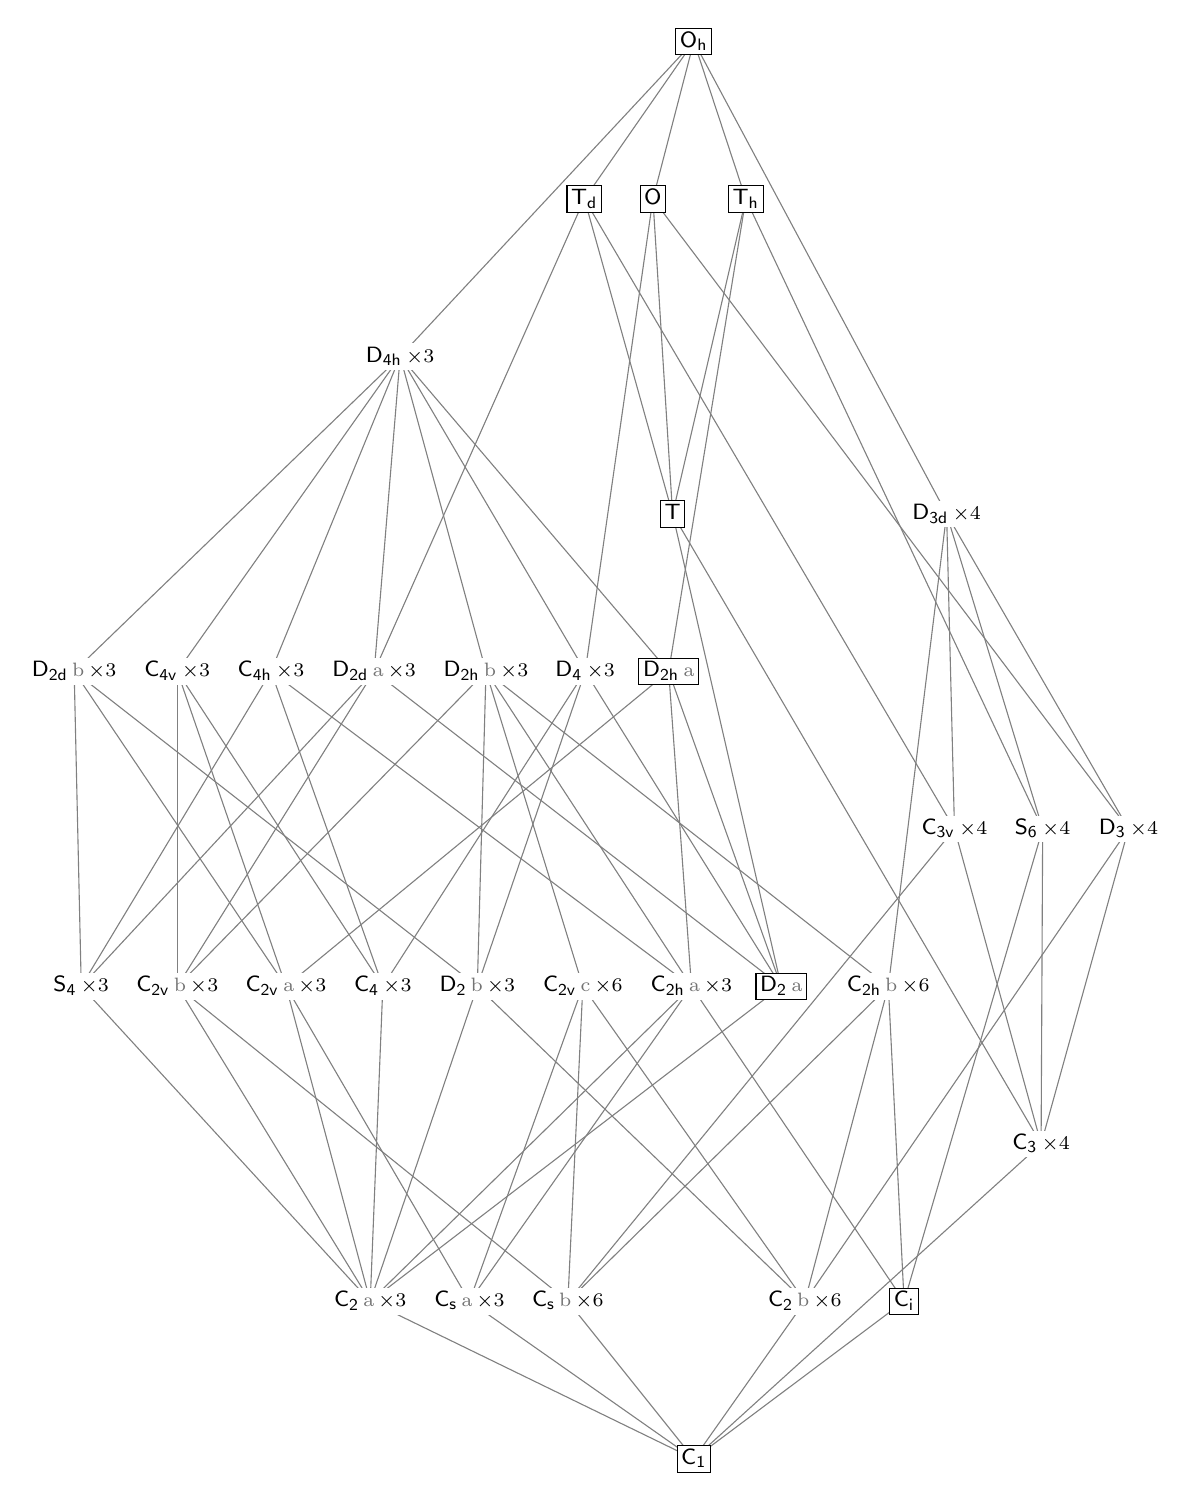
\begin{tikzpicture}[x=1cm, y=2.000cm,
  every node/.style={fill=white, font=\footnotesize, inner xsep=1.5pt, inner ysep=1.2pt, text height=5.6pt, text depth=1.6pt},
  normal/.style={draw, line width=0.4pt}, cover/.style={black!50, line width=0.4pt}]
\draw[cover] (0.00,0) -- (-4.11,1);
\draw[cover] (0.00,0) -- (1.41,1);
\draw[cover] (0.00,0) -- (2.67,1);
\draw[cover] (0.00,0) -- (-2.85,1);
\draw[cover] (0.00,0) -- (-1.60,1);
\draw[cover] (0.00,0) -- (4.41,2);
\draw[cover] (-4.11,1) -- (-3.95,3);
\draw[cover] (-4.11,1) -- (1.11,3);
\draw[cover] (-4.11,1) -- (-2.75,3);
\draw[cover] (-4.11,1) -- (-0.03,3);
\draw[cover] (-4.11,1) -- (-7.78,3);
\draw[cover] (-4.11,1) -- (-5.18,3);
\draw[cover] (-4.11,1) -- (-6.56,3);
\draw[cover] (1.41,1) -- (-2.75,3);
\draw[cover] (1.41,1) -- (2.47,3);
\draw[cover] (1.41,1) -- (-1.41,3);
\draw[cover] (1.41,1) -- (5.52,4);
\draw[cover] (2.67,1) -- (-0.03,3);
\draw[cover] (2.67,1) -- (2.47,3);
\draw[cover] (2.67,1) -- (4.43,4);
\draw[cover] (-2.85,1) -- (-0.03,3);
\draw[cover] (-2.85,1) -- (-5.18,3);
\draw[cover] (-2.85,1) -- (-1.41,3);
\draw[cover] (-1.60,1) -- (-6.56,3);
\draw[cover] (-1.60,1) -- (2.47,3);
\draw[cover] (-1.60,1) -- (-1.41,3);
\draw[cover] (-1.60,1) -- (3.31,4);
\draw[cover] (4.41,2) -- (5.52,4);
\draw[cover] (4.41,2) -- (4.43,4);
\draw[cover] (4.41,2) -- (3.31,4);
\draw[cover] (4.41,2) -- (-0.27,6);
\draw[cover] (-3.95,3) -- (-1.38,5);
\draw[cover] (-3.95,3) -- (-5.37,5);
\draw[cover] (-3.95,3) -- (-6.56,5);
\draw[cover] (1.11,3) -- (-1.38,5);
\draw[cover] (1.11,3) -- (-0.32,5);
\draw[cover] (1.11,3) -- (-4.06,5);
\draw[cover] (1.11,3) -- (-0.27,6);
\draw[cover] (-2.75,3) -- (-1.38,5);
\draw[cover] (-2.75,3) -- (-2.64,5);
\draw[cover] (-2.75,3) -- (-7.87,5);
\draw[cover] (-0.03,3) -- (-5.37,5);
\draw[cover] (-0.03,3) -- (-0.32,5);
\draw[cover] (-0.03,3) -- (-2.64,5);
\draw[cover] (-7.78,3) -- (-5.37,5);
\draw[cover] (-7.78,3) -- (-4.06,5);
\draw[cover] (-7.78,3) -- (-7.87,5);
\draw[cover] (-5.18,3) -- (-6.56,5);
\draw[cover] (-5.18,3) -- (-0.32,5);
\draw[cover] (-5.18,3) -- (-7.87,5);
\draw[cover] (-6.56,3) -- (-6.56,5);
\draw[cover] (-6.56,3) -- (-4.06,5);
\draw[cover] (-6.56,3) -- (-2.64,5);
\draw[cover] (2.47,3) -- (-2.64,5);
\draw[cover] (2.47,3) -- (3.21,6);
\draw[cover] (-1.41,3) -- (-2.64,5);
\draw[cover] (5.52,4) -- (3.21,6);
\draw[cover] (5.52,4) -- (-0.52,8);
\draw[cover] (4.43,4) -- (3.21,6);
\draw[cover] (4.43,4) -- (0.66,8);
\draw[cover] (3.31,4) -- (3.21,6);
\draw[cover] (3.31,4) -- (-1.39,8);
\draw[cover] (-1.38,5) -- (-3.73,7);
\draw[cover] (-1.38,5) -- (-0.52,8);
\draw[cover] (-5.37,5) -- (-3.73,7);
\draw[cover] (-6.56,5) -- (-3.73,7);
\draw[cover] (-0.32,5) -- (-3.73,7);
\draw[cover] (-0.32,5) -- (0.66,8);
\draw[cover] (-4.06,5) -- (-3.73,7);
\draw[cover] (-4.06,5) -- (-1.39,8);
\draw[cover] (-2.64,5) -- (-3.73,7);
\draw[cover] (-7.87,5) -- (-3.73,7);
\draw[cover] (-0.27,6) -- (-0.52,8);
\draw[cover] (-0.27,6) -- (0.66,8);
\draw[cover] (-0.27,6) -- (-1.39,8);
\draw[cover] (3.21,6) -- (0.00,9);
\draw[cover] (-3.73,7) -- (0.00,9);
\draw[cover] (-0.52,8) -- (0.00,9);
\draw[cover] (0.66,8) -- (0.00,9);
\draw[cover] (-1.39,8) -- (0.00,9);
\node[normal] (n00) at (0.00,0) {$\grp{C_{1}}$};
\node (n01) at (-4.11,1) {$\grp{C_{2}}$\clsletter{a}\,\nconj{3}};
\node (n02) at (1.41,1) {$\grp{C_{2}}$\clsletter{b}\,\nconj{6}};
\node[normal] (n03) at (2.67,1) {$\grp{C_{i}}$};
\node (n04) at (-2.85,1) {$\grp{C_{s}}$\clsletter{a}\,\nconj{3}};
\node (n05) at (-1.60,1) {$\grp{C_{s}}$\clsletter{b}\,\nconj{6}};
\node (n06) at (4.41,2) {$\grp{C_{3}}$\,\nconj{4}};
\node (n07) at (-3.95,3) {$\grp{C_{4}}$\,\nconj{3}};
\node[normal] (n08) at (1.11,3) {$\grp{D_{2}}$\clsletter{a}};
\node (n09) at (-2.75,3) {$\grp{D_{2}}$\clsletter{b}\,\nconj{3}};
\node (n10) at (-0.03,3) {$\grp{C_{2h}}$\clsletter{a}\,\nconj{3}};
\node (n11) at (-7.78,3) {$\grp{S_{4}}$\,\nconj{3}};
\node (n12) at (-5.18,3) {$\grp{C_{2v}}$\clsletter{a}\,\nconj{3}};
\node (n13) at (-6.56,3) {$\grp{C_{2v}}$\clsletter{b}\,\nconj{3}};
\node (n14) at (2.47,3) {$\grp{C_{2h}}$\clsletter{b}\,\nconj{6}};
\node (n15) at (-1.41,3) {$\grp{C_{2v}}$\clsletter{c}\,\nconj{6}};
\node (n16) at (5.52,4) {$\grp{D_{3}}$\,\nconj{4}};
\node (n17) at (4.43,4) {$\grp{S_{6}}$\,\nconj{4}};
\node (n18) at (3.31,4) {$\grp{C_{3v}}$\,\nconj{4}};
\node (n19) at (-1.38,5) {$\grp{D_{4}}$\,\nconj{3}};
\node (n20) at (-5.37,5) {$\grp{C_{4h}}$\,\nconj{3}};
\node (n21) at (-6.56,5) {$\grp{C_{4v}}$\,\nconj{3}};
\node[normal] (n22) at (-0.32,5) {$\grp{D_{2h}}$\clsletter{a}};
\node (n23) at (-4.06,5) {$\grp{D_{2d}}$\clsletter{a}\,\nconj{3}};
\node (n24) at (-2.64,5) {$\grp{D_{2h}}$\clsletter{b}\,\nconj{3}};
\node (n25) at (-7.87,5) {$\grp{D_{2d}}$\clsletter{b}\,\nconj{3}};
\node[normal] (n26) at (-0.27,6) {$\grp{T}$};
\node (n27) at (3.21,6) {$\grp{D_{3d}}$\,\nconj{4}};
\node (n28) at (-3.73,7) {$\grp{D_{4h}}$\,\nconj{3}};
\node[normal] (n29) at (-0.52,8) {$\grp{O}$};
\node[normal] (n30) at (0.66,8) {$\grp{T_{h}}$};
\node[normal] (n31) at (-1.39,8) {$\grp{T_{d}}$};
\node[normal] (n32) at (0.00,9) {$\grp{O_{h}}$};
\end{tikzpicture}
\end{center}
{\small\setlength{\fillwidth}{\textwidth}\addtolength{\fillwidth}{-12\tabcolsep}\setlength{\colwidth}{0pt}\cellmax{$\grp{C_{s}}$\clsletter{a} $\samecls$ $\grp{C_{1v}}$ $\samecls$ $\grp{C_{1h}}$}\cellmax{$\grp{C_{s}}$\clsletter{b} $\samecls$ $\grp{C_{1v}}$ $\samecls$ $\grp{C_{1h}}$}\cellmax{$\grp{C_{2h}}$\clsletter{a} $\samecls$ $\grp{D_{1d}}$}\cellmax{$\grp{C_{2h}}$\clsletter{b} $\samecls$ $\grp{D_{1d}}$}\cellmax{$\grp{C_{2v}}$\clsletter{a} $\samecls$ $\grp{D_{1h}}$}\cellmax{$\grp{C_{2v}}$\clsletter{b} $\samecls$ $\grp{D_{1h}}$}\cellmax{$\grp{C_{2v}}$\clsletter{c} $\samecls$ $\grp{D_{1h}}$}\cellmax{$\grp{C_{2}}$\clsletter{a} $\samecls$ $\grp{D_{1}}$}\cellmax{$\grp{C_{2}}$\clsletter{b} $\samecls$ $\grp{D_{1}}$}\cellmax{$\grp{C_{i}}$ $\samecls$ $\grp{S_{2}}$}\cellmax{subgrp}\cellmax{$\grp{D_{2d}}$\clsletter{a}}\cellmax{$\grp{D_{2d}}$\clsletter{b}}\cellmax{$\grp{D_{2h}}$\clsletter{a}}\cellmax{$\grp{D_{2h}}$\clsletter{b}}\cellmax{$\grp{C_{3v}}$}\cellmax{$\grp{C_{4h}}$}\cellmax{$\grp{C_{4v}}$}\cellmax{$\grp{D_{2}}$\clsletter{a}}\cellmax{$\grp{D_{2}}$\clsletter{b}}\cellmax{$\grp{D_{3d}}$}\cellmax{$\grp{D_{4h}}$}\cellmax{$\grp{C_{1}}$}\cellmax{$\grp{C_{3}}$}\cellmax{$\grp{C_{4}}$}\cellmax{$\grp{D_{3}}$}\cellmax{$\grp{D_{4}}$}\cellmax{$\grp{O_{h}}$}\cellmax{$\grp{S_{4}}$}\cellmax{$\grp{S_{6}}$}\cellmax{$\grp{T_{d}}$}\cellmax{$\grp{T_{h}}$}\cellmax{$\grp{O}$}\cellmax{$\grp{T}$}\addtolength{\fillwidth}{-\colwidth}\setlength{\colwidth}{0pt}\cellmax{order}\cellmax{12}\cellmax{16}\cellmax{24}\cellmax{48}\cellmax{1}\cellmax{2}\cellmax{3}\cellmax{4}\cellmax{6}\cellmax{8}\addtolength{\fillwidth}{-\colwidth}\setlength{\colwidth}{0pt}\cellmax{conjugates}\cellmax{1}\cellmax{3}\cellmax{4}\cellmax{6}\addtolength{\fillwidth}{-\colwidth}\setlength{\colwidth}{0pt}\cellmax{normal}\cellmax{yes}\cellmax{no}\addtolength{\fillwidth}{-\colwidth}\setlength{\colwidth}{0pt}\cellmax{$\grp{N}_{\hairsp \grp{O_{h}}}(\grp{H})$}\cellmax{$\grp{D_{2h}}$\clsletter{b}}\cellmax{$\grp{D_{3d}}$}\cellmax{$\grp{D_{4h}}$}\cellmax{$\grp{O_{h}}$}\addtolength{\fillwidth}{-\colwidth}\setlength{\colwidth}{0pt}\cellmax{$\grp{C}_{\hairsp \grp{O_{h}}}(\grp{H})$}\cellmax{$\grp{C_{2h}}$\clsletter{a}}\cellmax{$\grp{D_{2h}}$\clsletter{a}}\cellmax{$\grp{D_{2h}}$\clsletter{b}}\cellmax{$\grp{C_{4h}}$}\cellmax{$\grp{D_{4h}}$}\cellmax{$\grp{C_{i}}$}\cellmax{$\grp{O_{h}}$}\cellmax{$\grp{S_{6}}$}\addtolength{\fillwidth}{-\colwidth}\setlength{\colwidth}{0pt}\cellmax{$\cls{6C_{4}}$, $\cls{3C_{2}}$, $\cls{6C_{2}}$, $\cls{i}$, $\cls{6S_{4}}$, $\cls{3\sigma_{h}}$, $\cls{6\sigma_{d}}$}\cellmax{$\cls{3C_{2}}$, $\cls{6C_{2}}$, $\cls{i}$, $\cls{3\sigma_{h}}$, $\cls{6\sigma_{d}}$}\cellmax{$\cls{6C_{4}}$, $\cls{3C_{2}}$, $\cls{i}$, $\cls{6S_{4}}$, $\cls{3\sigma_{h}}$}\cellmax{$\cls{8C_{3}}$, $\cls{3C_{2}}$, $\cls{i}$, $\cls{8S_{6}}$, $\cls{3\sigma_{h}}$}\cellmax{$\cls{8C_{3}}$, $\cls{6C_{2}}$, $\cls{i}$, $\cls{8S_{6}}$, $\cls{6\sigma_{d}}$}\cellmax{$\cls{3C_{2}}$, $\cls{6C_{2}}$, $\cls{6S_{4}}$, $\cls{3\sigma_{h}}$}\cellmax{$\cls{6C_{4}}$, $\cls{3C_{2}}$, $\cls{3\sigma_{h}}$, $\cls{6\sigma_{d}}$}\cellmax{$\cls{6C_{4}}$, $\cls{8C_{3}}$, $\cls{3C_{2}}$, $\cls{6C_{2}}$}\cellmax{$\cls{8C_{3}}$, $\cls{3C_{2}}$, $\cls{6S_{4}}$, $\cls{6\sigma_{d}}$}\cellmax{$\cls{3C_{2}}$, $\cls{6S_{4}}$, $\cls{6\sigma_{d}}$}\cellmax{$\cls{6C_{2}}$, $\cls{3\sigma_{h}}$, $\cls{6\sigma_{d}}$}\cellmax{$\cls{6C_{4}}$, $\cls{3C_{2}}$, $\cls{6C_{2}}$}\cellmax{$\cls{3C_{2}}$, $\cls{i}$, $\cls{3\sigma_{h}}$}\cellmax{$\cls{6C_{2}}$, $\cls{i}$, $\cls{6\sigma_{d}}$}\cellmax{$\cls{8C_{3}}$, $\cls{i}$, $\cls{8S_{6}}$}\cellmax{$\cls{3C_{2}}$, $\cls{3\sigma_{h}}$}\cellmax{$\cls{3C_{2}}$, $\cls{6C_{2}}$}\cellmax{$\cls{3C_{2}}$, $\cls{6S_{4}}$}\cellmax{$\cls{3C_{2}}$, $\cls{6\sigma_{d}}$}\cellmax{$\cls{6C_{4}}$, $\cls{3C_{2}}$}\cellmax{$\cls{8C_{3}}$, $\cls{3C_{2}}$}\cellmax{$\cls{8C_{3}}$, $\cls{6C_{2}}$}\cellmax{$\cls{8C_{3}}$, $\cls{6\sigma_{d}}$}\cellmax{classes}\cellmax{$\cls{3C_{2}}$}\cellmax{$\cls{3\sigma_{h}}$}\cellmax{$\cls{6C_{2}}$}\cellmax{$\cls{6\sigma_{d}}$}\cellmax{$\cls{8C_{3}}$}\cellmax{---}\cellmax{all}\cellmax{$\cls{i}$}\fillcap\begin{longtable}{@{}lrrlll>{\RaggedRight\arraybackslash}p{\fillwidth}@{}}\toprule
subgrp & order & conjugates & normal & $\grp{N}_{\hairsp \grp{O_{h}}}(\grp{H})$ & $\grp{C}_{\hairsp \grp{O_{h}}}(\grp{H})$ & classes\\\midrule\endhead
\bottomrule\endfoot\endlastfoot
\href{C1.pdf}{$\grp{C_{1}}$} & 1 & 1 & yes & \href{Oh.pdf}{$\grp{O_{h}}$} & \href{Oh.pdf}{$\grp{O_{h}}$} & ---\\*
\href{C2.pdf}{$\grp{C_{2}}$}\clsletter{a} $\samecls$ \href{D1.pdf}{$\grp{D_{1}}$} & 2 & 3 & no & \href{D4h.pdf}{$\grp{D_{4h}}$} & \href{D4h.pdf}{$\grp{D_{4h}}$} & $\cls{3C_{2}}$\\
\href{C2.pdf}{$\grp{C_{2}}$}\clsletter{b} $\samecls$ \href{D1.pdf}{$\grp{D_{1}}$} & 2 & 6 & no & \href{D2h.pdf}{$\grp{D_{2h}}$}\clsletter{b} & \href{D2h.pdf}{$\grp{D_{2h}}$}\clsletter{b} & $\cls{6C_{2}}$\\
\href{S2.pdf}{$\grp{C_{i}}$} $\samecls$ \href{S2.pdf}{$\grp{S_{2}}$} & 2 & 1 & yes & \href{Oh.pdf}{$\grp{O_{h}}$} & \href{Oh.pdf}{$\grp{O_{h}}$} & $\cls{i}$\\
\href{C1v.pdf}{$\grp{C_{s}}$}\clsletter{a} $\samecls$ \href{C1v.pdf}{$\grp{C_{1v}}$} $\samecls$ \href{C1h.pdf}{$\grp{C_{1h}}$} & 2 & 3 & no & \href{D4h.pdf}{$\grp{D_{4h}}$} & \href{D4h.pdf}{$\grp{D_{4h}}$} & $\cls{3\sigma_{h}}$\\
\href{C1v.pdf}{$\grp{C_{s}}$}\clsletter{b} $\samecls$ \href{C1v.pdf}{$\grp{C_{1v}}$} $\samecls$ \href{C1h.pdf}{$\grp{C_{1h}}$} & 2 & 6 & no & \href{D2h.pdf}{$\grp{D_{2h}}$}\clsletter{b} & \href{D2h.pdf}{$\grp{D_{2h}}$}\clsletter{b} & $\cls{6\sigma_{d}}$\\
\href{C3.pdf}{$\grp{C_{3}}$} & 3 & 4 & no & \href{D3d.pdf}{$\grp{D_{3d}}$} & \href{S6.pdf}{$\grp{S_{6}}$} & $\cls{8C_{3}}$\\
\href{C4.pdf}{$\grp{C_{4}}$} & 4 & 3 & no & \href{D4h.pdf}{$\grp{D_{4h}}$} & \href{C4h.pdf}{$\grp{C_{4h}}$} & $\cls{6C_{4}}$, $\cls{3C_{2}}$\\
\href{S4.pdf}{$\grp{S_{4}}$} & 4 & 3 & no & \href{D4h.pdf}{$\grp{D_{4h}}$} & \href{C4h.pdf}{$\grp{C_{4h}}$} & $\cls{3C_{2}}$, $\cls{6S_{4}}$\\
\href{C2h.pdf}{$\grp{C_{2h}}$}\clsletter{a} $\samecls$ \href{D1d.pdf}{$\grp{D_{1d}}$} & 4 & 3 & no & \href{D4h.pdf}{$\grp{D_{4h}}$} & \href{D4h.pdf}{$\grp{D_{4h}}$} & $\cls{3C_{2}}$, $\cls{i}$, $\cls{3\sigma_{h}}$\\
\href{C2h.pdf}{$\grp{C_{2h}}$}\clsletter{b} $\samecls$ \href{D1d.pdf}{$\grp{D_{1d}}$} & 4 & 6 & no & \href{D2h.pdf}{$\grp{D_{2h}}$}\clsletter{b} & \href{D2h.pdf}{$\grp{D_{2h}}$}\clsletter{b} & $\cls{6C_{2}}$, $\cls{i}$, $\cls{6\sigma_{d}}$\\
\href{C2v.pdf}{$\grp{C_{2v}}$}\clsletter{a} $\samecls$ \href{D1h.pdf}{$\grp{D_{1h}}$} & 4 & 3 & no & \href{D4h.pdf}{$\grp{D_{4h}}$} & \href{D2h.pdf}{$\grp{D_{2h}}$}\clsletter{a} & $\cls{3C_{2}}$, $\cls{3\sigma_{h}}$\\
\href{C2v.pdf}{$\grp{C_{2v}}$}\clsletter{b} $\samecls$ \href{D1h.pdf}{$\grp{D_{1h}}$} & 4 & 3 & no & \href{D4h.pdf}{$\grp{D_{4h}}$} & \href{D2h.pdf}{$\grp{D_{2h}}$}\clsletter{b} & $\cls{3C_{2}}$, $\cls{6\sigma_{d}}$\\
\href{C2v.pdf}{$\grp{C_{2v}}$}\clsletter{c} $\samecls$ \href{D1h.pdf}{$\grp{D_{1h}}$} & 4 & 6 & no & \href{D2h.pdf}{$\grp{D_{2h}}$}\clsletter{b} & \href{D2h.pdf}{$\grp{D_{2h}}$}\clsletter{b} & $\cls{6C_{2}}$, $\cls{3\sigma_{h}}$, $\cls{6\sigma_{d}}$\\
\href{D2.pdf}{$\grp{D_{2}}$}\clsletter{a} & 4 & 1 & yes & \href{Oh.pdf}{$\grp{O_{h}}$} & \href{D2h.pdf}{$\grp{D_{2h}}$}\clsletter{a} & $\cls{3C_{2}}$\\
\href{D2.pdf}{$\grp{D_{2}}$}\clsletter{b} & 4 & 3 & no & \href{D4h.pdf}{$\grp{D_{4h}}$} & \href{D2h.pdf}{$\grp{D_{2h}}$}\clsletter{b} & $\cls{3C_{2}}$, $\cls{6C_{2}}$\\
\href{S6.pdf}{$\grp{S_{6}}$} & 6 & 4 & no & \href{D3d.pdf}{$\grp{D_{3d}}$} & \href{S6.pdf}{$\grp{S_{6}}$} & $\cls{8C_{3}}$, $\cls{i}$, $\cls{8S_{6}}$\\
\href{C3v.pdf}{$\grp{C_{3v}}$} & 6 & 4 & no & \href{D3d.pdf}{$\grp{D_{3d}}$} & \href{S2.pdf}{$\grp{C_{i}}$} & $\cls{8C_{3}}$, $\cls{6\sigma_{d}}$\\
\href{D3.pdf}{$\grp{D_{3}}$} & 6 & 4 & no & \href{D3d.pdf}{$\grp{D_{3d}}$} & \href{S2.pdf}{$\grp{C_{i}}$} & $\cls{8C_{3}}$, $\cls{6C_{2}}$\\
\href{C4h.pdf}{$\grp{C_{4h}}$} & 8 & 3 & no & \href{D4h.pdf}{$\grp{D_{4h}}$} & \href{C4h.pdf}{$\grp{C_{4h}}$} & $\cls{6C_{4}}$, $\cls{3C_{2}}$, $\cls{i}$, $\cls{6S_{4}}$, $\cls{3\sigma_{h}}$\\
\href{C4v.pdf}{$\grp{C_{4v}}$} & 8 & 3 & no & \href{D4h.pdf}{$\grp{D_{4h}}$} & \href{C2h.pdf}{$\grp{C_{2h}}$}\clsletter{a} & $\cls{6C_{4}}$, $\cls{3C_{2}}$, $\cls{3\sigma_{h}}$, $\cls{6\sigma_{d}}$\\
\href{D4.pdf}{$\grp{D_{4}}$} & 8 & 3 & no & \href{D4h.pdf}{$\grp{D_{4h}}$} & \href{C2h.pdf}{$\grp{C_{2h}}$}\clsletter{a} & $\cls{6C_{4}}$, $\cls{3C_{2}}$, $\cls{6C_{2}}$\\
\href{D2h.pdf}{$\grp{D_{2h}}$}\clsletter{a} & 8 & 1 & yes & \href{Oh.pdf}{$\grp{O_{h}}$} & \href{D2h.pdf}{$\grp{D_{2h}}$}\clsletter{a} & $\cls{3C_{2}}$, $\cls{i}$, $\cls{3\sigma_{h}}$\\
\href{D2h.pdf}{$\grp{D_{2h}}$}\clsletter{b} & 8 & 3 & no & \href{D4h.pdf}{$\grp{D_{4h}}$} & \href{D2h.pdf}{$\grp{D_{2h}}$}\clsletter{b} & $\cls{3C_{2}}$, $\cls{6C_{2}}$, $\cls{i}$, $\cls{3\sigma_{h}}$, $\cls{6\sigma_{d}}$\\
\href{D2d.pdf}{$\grp{D_{2d}}$}\clsletter{a} & 8 & 3 & no & \href{D4h.pdf}{$\grp{D_{4h}}$} & \href{C2h.pdf}{$\grp{C_{2h}}$}\clsletter{a} & $\cls{3C_{2}}$, $\cls{6S_{4}}$, $\cls{6\sigma_{d}}$\\
\href{D2d.pdf}{$\grp{D_{2d}}$}\clsletter{b} & 8 & 3 & no & \href{D4h.pdf}{$\grp{D_{4h}}$} & \href{C2h.pdf}{$\grp{C_{2h}}$}\clsletter{a} & $\cls{3C_{2}}$, $\cls{6C_{2}}$, $\cls{6S_{4}}$, $\cls{3\sigma_{h}}$\\
\href{D3d.pdf}{$\grp{D_{3d}}$} & 12 & 4 & no & \href{D3d.pdf}{$\grp{D_{3d}}$} & \href{S2.pdf}{$\grp{C_{i}}$} & $\cls{8C_{3}}$, $\cls{6C_{2}}$, $\cls{i}$, $\cls{8S_{6}}$, $\cls{6\sigma_{d}}$\\
\href{T.pdf}{$\grp{T}$} & 12 & 1 & yes & \href{Oh.pdf}{$\grp{O_{h}}$} & \href{S2.pdf}{$\grp{C_{i}}$} & $\cls{8C_{3}}$, $\cls{3C_{2}}$\\
\href{D4h.pdf}{$\grp{D_{4h}}$} & 16 & 3 & no & \href{D4h.pdf}{$\grp{D_{4h}}$} & \href{C2h.pdf}{$\grp{C_{2h}}$}\clsletter{a} & $\cls{6C_{4}}$, $\cls{3C_{2}}$, $\cls{6C_{2}}$, $\cls{i}$, $\cls{6S_{4}}$, $\cls{3\sigma_{h}}$, $\cls{6\sigma_{d}}$\\
\href{Th.pdf}{$\grp{T_{h}}$} & 24 & 1 & yes & \href{Oh.pdf}{$\grp{O_{h}}$} & \href{S2.pdf}{$\grp{C_{i}}$} & $\cls{8C_{3}}$, $\cls{3C_{2}}$, $\cls{i}$, $\cls{8S_{6}}$, $\cls{3\sigma_{h}}$\\
\href{Td.pdf}{$\grp{T_{d}}$} & 24 & 1 & yes & \href{Oh.pdf}{$\grp{O_{h}}$} & \href{S2.pdf}{$\grp{C_{i}}$} & $\cls{8C_{3}}$, $\cls{3C_{2}}$, $\cls{6S_{4}}$, $\cls{6\sigma_{d}}$\\
\href{O.pdf}{$\grp{O}$} & 24 & 1 & yes & \href{Oh.pdf}{$\grp{O_{h}}$} & \href{S2.pdf}{$\grp{C_{i}}$} & $\cls{6C_{4}}$, $\cls{8C_{3}}$, $\cls{3C_{2}}$, $\cls{6C_{2}}$\\*
\href{Oh.pdf}{$\grp{O_{h}}$} & 48 & 1 & yes & \href{Oh.pdf}{$\grp{O_{h}}$} & \href{S2.pdf}{$\grp{C_{i}}$} & all\\
\bottomrule\end{longtable}}
\needspace{103pt}
\section{Descent of symmetry}\label{s:subduction}
Conventions: \href{../../CONVENTIONS.pdf}{CONVENTIONS.pdf}, sections \href{../../CONVENTIONS.pdf\#conv.12.2}{12.2} and \href{../../CONVENTIONS.pdf\#conv.12.4}{12.4}.
A column is a class of subgroups $\grp{H}$, in the order of the table of section~\ref{s:subgroups}. The row subgrp names it by its symbol, as in that table, with the letter that distinguishes classes with the same symbol, which are not conjugate in $\grp{O_{h}}$. The symbol links to the document of $\grp{H}$. The entry of row $\Gamma$ is $\restr{\Gamma}{\grp{H}}$, the restriction of $\Gamma$ along a monomorphism from the record of $\grp{H}$ onto the subgroup, as a sum of the irreps of $\grp{H}$. The monomorphism identifies the subgroup with its record, and $\grp{H}$ names both. \label{n:group.normalizer.o3}\label{n:group.centralizer.o3}The record of $\grp{H}$ maps onto the subgroup in $\grpindex{\grp{N}}{\grp{C}}$ ways, $h \mapsto g h g^{-1}$ ($h \in \grp{H}$) for the $g \in \grp{O(3)}$ that carry $\grp{H}$ to it. Here $\grp{N}$ and $\grp{C}$ are the normalizer and centralizer of $\grp{H}$ in \href{O3.pdf}{$\grp{O(3)}$}. In the section Names and structure of the document of $\grp{H}$, the row centralizer gives $\grp{C}$ and the index $\grpindex{\grp{N}}{\grp{C}}$ (the index in the row normalizer is $\grpindex{\grp{N}}{\grp{H}}$). Two maps related by a conjugation in $\grp{O_{h}}$ give the same restriction. Thus the maps fall into $\grpindex{\grp{N}}{\grp{C}}/\grpindex{\grp{N}_{\hairsp \grp{O_{h}}}}{\grp{C}_{\hairsp \grp{O_{h}}}}$ classes, where $\grp{N}_{\hairsp \grp{O_{h}}}$ and $\grp{C}_{\hairsp \grp{O_{h}}}$ are the normalizer and centralizer of the subgroup in $\grp{O_{h}}$ (the table of section~\ref{s:subgroups}). \label{n:head.setting}A subgroup whose classes of maps give different tables has one column for each table: setting 1 for the stored monomorphism (\texttt{monomorphism}) and settings 2, 3, \dots{} for the \texttt{alternative\symbol{95}settings}. Each setting has the images of the generators of $\grp{H}$ (\texttt{setting}). \label{n:head.images}The row images gives, under each setting, each generator whose image differs between the settings, in their order, mapped to the class of $\grp{O_{h}}$ that contains its image. \label{n:element.generator.index}Each generator is written by the symbol of its class (\href{../../CONVENTIONS.pdf}{CONVENTIONS.pdf}, section \href{../../CONVENTIONS.pdf\#conv.5.1}{5.1}), and where two share a symbol, a superscript number in brackets gives the generator's index in the document of $\grp{H}$. \label{n:irrep.Delta}Each other setting is setting 1 with each irrep $\Lambda$ of $\grp{H}$ replaced by $\Lambda$ composed with one automorphism of $\grp{H}$ induced by a conjugation in \href{O3.pdf}{$\grp{O(3)}$} and by none in $\grp{O_{h}}$ (\href{../../CONVENTIONS.pdf}{CONVENTIONS.pdf}, section \href{../../CONVENTIONS.pdf\#conv.12.1}{12.1}).
{\small\begin{longtable}{@{}lcccccccc@{}}\toprule
subgrp & \href{C2.pdf}{$\grp{C_{2}}$}\clsletter{a} & \href{C2.pdf}{$\grp{C_{2}}$}\clsletter{b} & \href{S2.pdf}{$\grp{C_{i}}$} & \href{C1v.pdf}{$\grp{C_{s}}$}\clsletter{a} & \href{C1v.pdf}{$\grp{C_{s}}$}\clsletter{b} & \href{C3.pdf}{$\grp{C_{3}}$} & \href{C4.pdf}{$\grp{C_{4}}$} & \href{S4.pdf}{$\grp{S_{4}}$}\\\midrule\endhead
\bottomrule\endfoot\endlastfoot
$\irr{a}_{1\ptag{g}}$ & $\irr{a}$ & $\irr{a}$ & $\irr{a}_{\ptag{g}}$ & $\irr{a}'$ & $\irr{a}'$ & $\irr{a}$ & $\irr{a}$ & $\irr{a}$\\*
$\irr{a}_{2\ptag{g}}$ & $\irr{a}$ & $\irr{b}$ & $\irr{a}_{\ptag{g}}$ & $\irr{a}'$ & $\irr{a}''$ & $\irr{a}$ & $\irr{b}$ & $\irr{b}$\\*
$\irr{e}_{\ptag{g}}$ & $2\,\irr{a}$ & $\irr{a}\oplus \irr{b}$ & $2\,\irr{a}_{\ptag{g}}$ & $2\,\irr{a}'$ & $\irr{a}'\oplus \irr{a}''$ & $\conjpair{1}\irr{e}\oplus \conjpair{2}\irr{e}$ & $\irr{a}\oplus \irr{b}$ & $\irr{a}\oplus \irr{b}$\\*
$\irr{t}_{1\ptag{g}}$ & $\irr{a}\oplus 2\,\irr{b}$ & $\irr{a}\oplus 2\,\irr{b}$ & $3\,\irr{a}_{\ptag{g}}$ & $\irr{a}'\oplus 2\,\irr{a}''$ & $\irr{a}'\oplus 2\,\irr{a}''$ & $\irr{a}\oplus \conjpair{1}\irr{e}\oplus \conjpair{2}\irr{e}$ & $\irr{a}\oplus \conjpair{1}\irr{e}\oplus \conjpair{2}\irr{e}$ & $\irr{a}\oplus \conjpair{1}\irr{e}\oplus \conjpair{2}\irr{e}$\\*
$\irr{t}_{2\ptag{g}}$ & $\irr{a}\oplus 2\,\irr{b}$ & $2\,\irr{a}\oplus \irr{b}$ & $3\,\irr{a}_{\ptag{g}}$ & $\irr{a}'\oplus 2\,\irr{a}''$ & $2\,\irr{a}'\oplus \irr{a}''$ & $\irr{a}\oplus \conjpair{1}\irr{e}\oplus \conjpair{2}\irr{e}$ & $\irr{b}\oplus \conjpair{1}\irr{e}\oplus \conjpair{2}\irr{e}$ & $\irr{b}\oplus \conjpair{1}\irr{e}\oplus \conjpair{2}\irr{e}$\\*
$\irr{a}_{1\ptag{u}}$ & $\irr{a}$ & $\irr{a}$ & $\irr{a}_{\ptag{u}}$ & $\irr{a}''$ & $\irr{a}''$ & $\irr{a}$ & $\irr{a}$ & $\irr{b}$\\*
$\irr{a}_{2\ptag{u}}$ & $\irr{a}$ & $\irr{b}$ & $\irr{a}_{\ptag{u}}$ & $\irr{a}''$ & $\irr{a}'$ & $\irr{a}$ & $\irr{b}$ & $\irr{a}$\\*
$\irr{e}_{\ptag{u}}$ & $2\,\irr{a}$ & $\irr{a}\oplus \irr{b}$ & $2\,\irr{a}_{\ptag{u}}$ & $2\,\irr{a}''$ & $\irr{a}'\oplus \irr{a}''$ & $\conjpair{1}\irr{e}\oplus \conjpair{2}\irr{e}$ & $\irr{a}\oplus \irr{b}$ & $\irr{a}\oplus \irr{b}$\\*
$\irr{t}_{1\ptag{u}}$ & $\irr{a}\oplus 2\,\irr{b}$ & $\irr{a}\oplus 2\,\irr{b}$ & $3\,\irr{a}_{\ptag{u}}$ & $2\,\irr{a}'\oplus \irr{a}''$ & $2\,\irr{a}'\oplus \irr{a}''$ & $\irr{a}\oplus \conjpair{1}\irr{e}\oplus \conjpair{2}\irr{e}$ & $\irr{a}\oplus \conjpair{1}\irr{e}\oplus \conjpair{2}\irr{e}$ & $\irr{b}\oplus \conjpair{1}\irr{e}\oplus \conjpair{2}\irr{e}$\\*
$\irr{t}_{2\ptag{u}}$ & $\irr{a}\oplus 2\,\irr{b}$ & $2\,\irr{a}\oplus \irr{b}$ & $3\,\irr{a}_{\ptag{u}}$ & $2\,\irr{a}'\oplus \irr{a}''$ & $\irr{a}'\oplus 2\,\irr{a}''$ & $\irr{a}\oplus \conjpair{1}\irr{e}\oplus \conjpair{2}\irr{e}$ & $\irr{b}\oplus \conjpair{1}\irr{e}\oplus \conjpair{2}\irr{e}$ & $\irr{a}\oplus \conjpair{1}\irr{e}\oplus \conjpair{2}\irr{e}$\\
\bottomrule\end{longtable}}
{\small\begin{longtable}{@{}lcccccc@{}}\toprule
subgrp & \href{C2h.pdf}{$\grp{C_{2h}}$}\clsletter{a} & \href{C2h.pdf}{$\grp{C_{2h}}$}\clsletter{b} & \href{C2v.pdf}{$\grp{C_{2v}}$}\clsletter{a} & \href{C2v.pdf}{$\grp{C_{2v}}$}\clsletter{b} & \multicolumn{2}{c}{\href{C2v.pdf}{$\grp{C_{2v}}$}\clsletter{c}}\\\cmidrule(lr){6-7}
setting &  &  &  &  & 1 & 2\\
images &  &  &  &  & {\scriptsize $\cls{\sigma_{v}} \mapsto \cls{3\sigma_{h}}$} & {\scriptsize $\cls{\sigma_{v}} \mapsto \cls{6\sigma_{d}}$}\\\midrule\endhead
\bottomrule\endfoot\endlastfoot
$\irr{a}_{1\ptag{g}}$ & $\irr{a}_{\ptag{g}}$ & $\irr{a}_{\ptag{g}}$ & $\irr{a}_{1}$ & $\irr{a}_{1}$ & $\irr{a}_{1}$ & $\irr{a}_{1}$\\*
$\irr{a}_{2\ptag{g}}$ & $\irr{a}_{\ptag{g}}$ & $\irr{b}_{\ptag{g}}$ & $\irr{a}_{1}$ & $\irr{a}_{2}$ & $\irr{b}_{1}$ & $\irr{b}_{2}$\\*
$\irr{e}_{\ptag{g}}$ & $2\,\irr{a}_{\ptag{g}}$ & $\irr{a}_{\ptag{g}}\oplus \irr{b}_{\ptag{g}}$ & $2\,\irr{a}_{1}$ & $\irr{a}_{1}\oplus \irr{a}_{2}$ & $\irr{a}_{1}\oplus \irr{b}_{1}$ & $\irr{a}_{1}\oplus \irr{b}_{2}$\\*
$\irr{t}_{1\ptag{g}}$ & $\irr{a}_{\ptag{g}}\oplus 2\,\irr{b}_{\ptag{g}}$ & $\irr{a}_{\ptag{g}}\oplus 2\,\irr{b}_{\ptag{g}}$ & $\irr{a}_{2}\oplus \irr{b}_{1}\oplus \irr{b}_{2}$ & $\irr{a}_{2}\oplus \irr{b}_{1}\oplus \irr{b}_{2}$ & $\irr{a}_{2}\oplus \irr{b}_{1}\oplus \irr{b}_{2}$ & $\irr{a}_{2}\oplus \irr{b}_{1}\oplus \irr{b}_{2}$\\*
$\irr{t}_{2\ptag{g}}$ & $\irr{a}_{\ptag{g}}\oplus 2\,\irr{b}_{\ptag{g}}$ & $2\,\irr{a}_{\ptag{g}}\oplus \irr{b}_{\ptag{g}}$ & $\irr{a}_{2}\oplus \irr{b}_{1}\oplus \irr{b}_{2}$ & $\irr{a}_{1}\oplus \irr{b}_{1}\oplus \irr{b}_{2}$ & $\irr{a}_{1}\oplus \irr{a}_{2}\oplus \irr{b}_{2}$ & $\irr{a}_{1}\oplus \irr{a}_{2}\oplus \irr{b}_{1}$\\*
$\irr{a}_{1\ptag{u}}$ & $\irr{a}_{\ptag{u}}$ & $\irr{a}_{\ptag{u}}$ & $\irr{a}_{2}$ & $\irr{a}_{2}$ & $\irr{a}_{2}$ & $\irr{a}_{2}$\\*
$\irr{a}_{2\ptag{u}}$ & $\irr{a}_{\ptag{u}}$ & $\irr{b}_{\ptag{u}}$ & $\irr{a}_{2}$ & $\irr{a}_{1}$ & $\irr{b}_{2}$ & $\irr{b}_{1}$\\*
$\irr{e}_{\ptag{u}}$ & $2\,\irr{a}_{\ptag{u}}$ & $\irr{a}_{\ptag{u}}\oplus \irr{b}_{\ptag{u}}$ & $2\,\irr{a}_{2}$ & $\irr{a}_{1}\oplus \irr{a}_{2}$ & $\irr{a}_{2}\oplus \irr{b}_{2}$ & $\irr{a}_{2}\oplus \irr{b}_{1}$\\*
$\irr{t}_{1\ptag{u}}$ & $\irr{a}_{\ptag{u}}\oplus 2\,\irr{b}_{\ptag{u}}$ & $\irr{a}_{\ptag{u}}\oplus 2\,\irr{b}_{\ptag{u}}$ & $\irr{a}_{1}\oplus \irr{b}_{1}\oplus \irr{b}_{2}$ & $\irr{a}_{1}\oplus \irr{b}_{1}\oplus \irr{b}_{2}$ & $\irr{a}_{1}\oplus \irr{b}_{1}\oplus \irr{b}_{2}$ & $\irr{a}_{1}\oplus \irr{b}_{1}\oplus \irr{b}_{2}$\\*
$\irr{t}_{2\ptag{u}}$ & $\irr{a}_{\ptag{u}}\oplus 2\,\irr{b}_{\ptag{u}}$ & $2\,\irr{a}_{\ptag{u}}\oplus \irr{b}_{\ptag{u}}$ & $\irr{a}_{1}\oplus \irr{b}_{1}\oplus \irr{b}_{2}$ & $\irr{a}_{2}\oplus \irr{b}_{1}\oplus \irr{b}_{2}$ & $\irr{a}_{1}\oplus \irr{a}_{2}\oplus \irr{b}_{1}$ & $\irr{a}_{1}\oplus \irr{a}_{2}\oplus \irr{b}_{2}$\\
\bottomrule\end{longtable}}
{\small\begin{longtable}{@{}lccccccc@{}}\toprule
subgrp & \href{D2.pdf}{$\grp{D_{2}}$}\clsletter{a} & \multicolumn{3}{c}{\href{D2.pdf}{$\grp{D_{2}}$}\clsletter{b}} & \href{S6.pdf}{$\grp{S_{6}}$} & \href{C3v.pdf}{$\grp{C_{3v}}$} & \href{D3.pdf}{$\grp{D_{3}}$}\\\cmidrule(lr){3-5}
setting &  & 1 & 2 & 3 &  &  & \\
images &  & {\scriptsize\begin{tabular}[t]{@{}c@{}}$\cls{\genidx{C_{2}}{1}} \mapsto \cls{3C_{2}}$\\$\cls{\genidx{C_{2}}{2}} \mapsto \cls{6C_{2}}$\end{tabular}} & {\scriptsize\begin{tabular}[t]{@{}c@{}}$\cls{\genidx{C_{2}}{1}} \mapsto \cls{6C_{2}}$\\$\cls{\genidx{C_{2}}{2}} \mapsto \cls{3C_{2}}$\end{tabular}} & {\scriptsize\begin{tabular}[t]{@{}c@{}}$\cls{\genidx{C_{2}}{1}} \mapsto \cls{6C_{2}}$\\$\cls{\genidx{C_{2}}{2}} \mapsto \cls{6C_{2}}$\end{tabular}} &  &  & \\\midrule\endhead
\bottomrule\endfoot\endlastfoot
$\irr{a}_{1\ptag{g}}$ & $\irr{a}$ & $\irr{a}$ & $\irr{a}$ & $\irr{a}$ & $\irr{a}_{\ptag{g}}$ & $\irr{a}_{1}$ & $\irr{a}_{1}$\\*
$\irr{a}_{2\ptag{g}}$ & $\irr{a}$ & $\irr{b}_{1}$ & $\irr{b}_{3}$ & $\irr{b}_{2}$ & $\irr{a}_{\ptag{g}}$ & $\irr{a}_{2}$ & $\irr{a}_{2}$\\*
$\irr{e}_{\ptag{g}}$ & $2\,\irr{a}$ & $\irr{a}\oplus \irr{b}_{1}$ & $\irr{a}\oplus \irr{b}_{3}$ & $\irr{a}\oplus \irr{b}_{2}$ & $\conjpair{1}\irr{e}_{\ptag{g}}\oplus \conjpair{2}\irr{e}_{\ptag{g}}$ & $\irr{e}$ & $\irr{e}$\\*
$\irr{t}_{1\ptag{g}}$ & $\irr{b}_{1}\oplus \irr{b}_{2}\oplus \irr{b}_{3}$ & $\irr{b}_{1}\oplus \irr{b}_{2}\oplus \irr{b}_{3}$ & $\irr{b}_{1}\oplus \irr{b}_{2}\oplus \irr{b}_{3}$ & $\irr{b}_{1}\oplus \irr{b}_{2}\oplus \irr{b}_{3}$ & $\irr{a}_{\ptag{g}}\oplus \conjpair{1}\irr{e}_{\ptag{g}}\oplus \conjpair{2}\irr{e}_{\ptag{g}}$ & $\irr{a}_{2}\oplus \irr{e}$ & $\irr{a}_{2}\oplus \irr{e}$\\*
$\irr{t}_{2\ptag{g}}$ & $\irr{b}_{1}\oplus \irr{b}_{2}\oplus \irr{b}_{3}$ & $\irr{a}\oplus \irr{b}_{2}\oplus \irr{b}_{3}$ & $\irr{a}\oplus \irr{b}_{1}\oplus \irr{b}_{2}$ & $\irr{a}\oplus \irr{b}_{1}\oplus \irr{b}_{3}$ & $\irr{a}_{\ptag{g}}\oplus \conjpair{1}\irr{e}_{\ptag{g}}\oplus \conjpair{2}\irr{e}_{\ptag{g}}$ & $\irr{a}_{1}\oplus \irr{e}$ & $\irr{a}_{1}\oplus \irr{e}$\\*
$\irr{a}_{1\ptag{u}}$ & $\irr{a}$ & $\irr{a}$ & $\irr{a}$ & $\irr{a}$ & $\irr{a}_{\ptag{u}}$ & $\irr{a}_{2}$ & $\irr{a}_{1}$\\*
$\irr{a}_{2\ptag{u}}$ & $\irr{a}$ & $\irr{b}_{1}$ & $\irr{b}_{3}$ & $\irr{b}_{2}$ & $\irr{a}_{\ptag{u}}$ & $\irr{a}_{1}$ & $\irr{a}_{2}$\\*
$\irr{e}_{\ptag{u}}$ & $2\,\irr{a}$ & $\irr{a}\oplus \irr{b}_{1}$ & $\irr{a}\oplus \irr{b}_{3}$ & $\irr{a}\oplus \irr{b}_{2}$ & $\conjpair{1}\irr{e}_{\ptag{u}}\oplus \conjpair{2}\irr{e}_{\ptag{u}}$ & $\irr{e}$ & $\irr{e}$\\*
$\irr{t}_{1\ptag{u}}$ & $\irr{b}_{1}\oplus \irr{b}_{2}\oplus \irr{b}_{3}$ & $\irr{b}_{1}\oplus \irr{b}_{2}\oplus \irr{b}_{3}$ & $\irr{b}_{1}\oplus \irr{b}_{2}\oplus \irr{b}_{3}$ & $\irr{b}_{1}\oplus \irr{b}_{2}\oplus \irr{b}_{3}$ & $\irr{a}_{\ptag{u}}\oplus \conjpair{1}\irr{e}_{\ptag{u}}\oplus \conjpair{2}\irr{e}_{\ptag{u}}$ & $\irr{a}_{1}\oplus \irr{e}$ & $\irr{a}_{2}\oplus \irr{e}$\\*
$\irr{t}_{2\ptag{u}}$ & $\irr{b}_{1}\oplus \irr{b}_{2}\oplus \irr{b}_{3}$ & $\irr{a}\oplus \irr{b}_{2}\oplus \irr{b}_{3}$ & $\irr{a}\oplus \irr{b}_{1}\oplus \irr{b}_{2}$ & $\irr{a}\oplus \irr{b}_{1}\oplus \irr{b}_{3}$ & $\irr{a}_{\ptag{u}}\oplus \conjpair{1}\irr{e}_{\ptag{u}}\oplus \conjpair{2}\irr{e}_{\ptag{u}}$ & $\irr{a}_{2}\oplus \irr{e}$ & $\irr{a}_{1}\oplus \irr{e}$\\
\bottomrule\end{longtable}}
{\small\begin{longtable}{@{}lcccccc@{}}\toprule
subgrp & \href{C4h.pdf}{$\grp{C_{4h}}$} & \multicolumn{2}{c}{\href{C4v.pdf}{$\grp{C_{4v}}$}} & \multicolumn{2}{c}{\href{D4.pdf}{$\grp{D_{4}}$}} & \href{D2h.pdf}{$\grp{D_{2h}}$}\clsletter{a}\\\cmidrule(lr){3-4}\cmidrule(lr){5-6}
setting &  & 1 & 2 & 1 & 2 & \\
images &  & {\scriptsize $\cls{\sigma_{v}} \mapsto \cls{3\sigma_{h}}$} & {\scriptsize $\cls{\sigma_{v}} \mapsto \cls{6\sigma_{d}}$} & {\scriptsize $\cls{C_{2}} \mapsto \cls{3C_{2}}$} & {\scriptsize $\cls{C_{2}} \mapsto \cls{6C_{2}}$} & \\\midrule\endhead
\bottomrule\endfoot\endlastfoot
$\irr{a}_{1\ptag{g}}$ & $\irr{a}_{\ptag{g}}$ & $\irr{a}_{1}$ & $\irr{a}_{1}$ & $\irr{a}_{1}$ & $\irr{a}_{1}$ & $\irr{a}_{\ptag{g}}$\\*
$\irr{a}_{2\ptag{g}}$ & $\irr{b}_{\ptag{g}}$ & $\irr{b}_{1}$ & $\irr{b}_{2}$ & $\irr{b}_{1}$ & $\irr{b}_{2}$ & $\irr{a}_{\ptag{g}}$\\*
$\irr{e}_{\ptag{g}}$ & $\irr{a}_{\ptag{g}}\oplus \irr{b}_{\ptag{g}}$ & $\irr{a}_{1}\oplus \irr{b}_{1}$ & $\irr{a}_{1}\oplus \irr{b}_{2}$ & $\irr{a}_{1}\oplus \irr{b}_{1}$ & $\irr{a}_{1}\oplus \irr{b}_{2}$ & $2\,\irr{a}_{\ptag{g}}$\\*
$\irr{t}_{1\ptag{g}}$ & $\irr{a}_{\ptag{g}}\oplus \conjpair{1}\irr{e}_{\ptag{g}}\oplus \conjpair{2}\irr{e}_{\ptag{g}}$ & $\irr{a}_{2}\oplus \irr{e}$ & $\irr{a}_{2}\oplus \irr{e}$ & $\irr{a}_{2}\oplus \irr{e}$ & $\irr{a}_{2}\oplus \irr{e}$ & $\irr{b}_{1\ptag{g}}\oplus \irr{b}_{2\ptag{g}}\oplus \irr{b}_{3\ptag{g}}$\\*
$\irr{t}_{2\ptag{g}}$ & $\irr{b}_{\ptag{g}}\oplus \conjpair{1}\irr{e}_{\ptag{g}}\oplus \conjpair{2}\irr{e}_{\ptag{g}}$ & $\irr{b}_{2}\oplus \irr{e}$ & $\irr{b}_{1}\oplus \irr{e}$ & $\irr{b}_{2}\oplus \irr{e}$ & $\irr{b}_{1}\oplus \irr{e}$ & $\irr{b}_{1\ptag{g}}\oplus \irr{b}_{2\ptag{g}}\oplus \irr{b}_{3\ptag{g}}$\\*
$\irr{a}_{1\ptag{u}}$ & $\irr{a}_{\ptag{u}}$ & $\irr{a}_{2}$ & $\irr{a}_{2}$ & $\irr{a}_{1}$ & $\irr{a}_{1}$ & $\irr{a}_{\ptag{u}}$\\*
$\irr{a}_{2\ptag{u}}$ & $\irr{b}_{\ptag{u}}$ & $\irr{b}_{2}$ & $\irr{b}_{1}$ & $\irr{b}_{1}$ & $\irr{b}_{2}$ & $\irr{a}_{\ptag{u}}$\\*
$\irr{e}_{\ptag{u}}$ & $\irr{a}_{\ptag{u}}\oplus \irr{b}_{\ptag{u}}$ & $\irr{a}_{2}\oplus \irr{b}_{2}$ & $\irr{a}_{2}\oplus \irr{b}_{1}$ & $\irr{a}_{1}\oplus \irr{b}_{1}$ & $\irr{a}_{1}\oplus \irr{b}_{2}$ & $2\,\irr{a}_{\ptag{u}}$\\*
$\irr{t}_{1\ptag{u}}$ & $\irr{a}_{\ptag{u}}\oplus \conjpair{1}\irr{e}_{\ptag{u}}\oplus \conjpair{2}\irr{e}_{\ptag{u}}$ & $\irr{a}_{1}\oplus \irr{e}$ & $\irr{a}_{1}\oplus \irr{e}$ & $\irr{a}_{2}\oplus \irr{e}$ & $\irr{a}_{2}\oplus \irr{e}$ & $\irr{b}_{1\ptag{u}}\oplus \irr{b}_{2\ptag{u}}\oplus \irr{b}_{3\ptag{u}}$\\*
$\irr{t}_{2\ptag{u}}$ & $\irr{b}_{\ptag{u}}\oplus \conjpair{1}\irr{e}_{\ptag{u}}\oplus \conjpair{2}\irr{e}_{\ptag{u}}$ & $\irr{b}_{1}\oplus \irr{e}$ & $\irr{b}_{2}\oplus \irr{e}$ & $\irr{b}_{2}\oplus \irr{e}$ & $\irr{b}_{1}\oplus \irr{e}$ & $\irr{b}_{1\ptag{u}}\oplus \irr{b}_{2\ptag{u}}\oplus \irr{b}_{3\ptag{u}}$\\
\bottomrule\end{longtable}}
{\small\begin{longtable}{@{}lcccccc@{}}\toprule
subgrp & \multicolumn{3}{c}{\href{D2h.pdf}{$\grp{D_{2h}}$}\clsletter{b}} & \href{D2d.pdf}{$\grp{D_{2d}}$}\clsletter{a} & \href{D2d.pdf}{$\grp{D_{2d}}$}\clsletter{b} & \href{D3d.pdf}{$\grp{D_{3d}}$}\\\cmidrule(lr){2-4}
setting & 1 & 2 & 3 &  &  & \\
images & {\scriptsize\begin{tabular}[t]{@{}c@{}}$\cls{\genidx{C_{2}}{1}} \mapsto \cls{3C_{2}}$\\$\cls{\genidx{C_{2}}{2}} \mapsto \cls{6C_{2}}$\end{tabular}} & {\scriptsize\begin{tabular}[t]{@{}c@{}}$\cls{\genidx{C_{2}}{1}} \mapsto \cls{6C_{2}}$\\$\cls{\genidx{C_{2}}{2}} \mapsto \cls{3C_{2}}$\end{tabular}} & {\scriptsize\begin{tabular}[t]{@{}c@{}}$\cls{\genidx{C_{2}}{1}} \mapsto \cls{6C_{2}}$\\$\cls{\genidx{C_{2}}{2}} \mapsto \cls{6C_{2}}$\end{tabular}} &  &  & \\\midrule\endhead
\bottomrule\endfoot\endlastfoot
$\irr{a}_{1\ptag{g}}$ & $\irr{a}_{\ptag{g}}$ & $\irr{a}_{\ptag{g}}$ & $\irr{a}_{\ptag{g}}$ & $\irr{a}_{1}$ & $\irr{a}_{1}$ & $\irr{a}_{1\ptag{g}}$\\*
$\irr{a}_{2\ptag{g}}$ & $\irr{b}_{1\ptag{g}}$ & $\irr{b}_{3\ptag{g}}$ & $\irr{b}_{2\ptag{g}}$ & $\irr{b}_{1}$ & $\irr{b}_{2}$ & $\irr{a}_{2\ptag{g}}$\\*
$\irr{e}_{\ptag{g}}$ & $\irr{a}_{\ptag{g}}\oplus \irr{b}_{1\ptag{g}}$ & $\irr{a}_{\ptag{g}}\oplus \irr{b}_{3\ptag{g}}$ & $\irr{a}_{\ptag{g}}\oplus \irr{b}_{2\ptag{g}}$ & $\irr{a}_{1}\oplus \irr{b}_{1}$ & $\irr{a}_{1}\oplus \irr{b}_{2}$ & $\irr{e}_{\ptag{g}}$\\*
$\irr{t}_{1\ptag{g}}$ & $\irr{b}_{1\ptag{g}}\oplus \irr{b}_{2\ptag{g}}\oplus \irr{b}_{3\ptag{g}}$ & $\irr{b}_{1\ptag{g}}\oplus \irr{b}_{2\ptag{g}}\oplus \irr{b}_{3\ptag{g}}$ & $\irr{b}_{1\ptag{g}}\oplus \irr{b}_{2\ptag{g}}\oplus \irr{b}_{3\ptag{g}}$ & $\irr{a}_{2}\oplus \irr{e}$ & $\irr{a}_{2}\oplus \irr{e}$ & $\irr{a}_{2\ptag{g}}\oplus \irr{e}_{\ptag{g}}$\\*
$\irr{t}_{2\ptag{g}}$ & $\irr{a}_{\ptag{g}}\oplus \irr{b}_{2\ptag{g}}\oplus \irr{b}_{3\ptag{g}}$ & $\irr{a}_{\ptag{g}}\oplus \irr{b}_{1\ptag{g}}\oplus \irr{b}_{2\ptag{g}}$ & $\irr{a}_{\ptag{g}}\oplus \irr{b}_{1\ptag{g}}\oplus \irr{b}_{3\ptag{g}}$ & $\irr{b}_{2}\oplus \irr{e}$ & $\irr{b}_{1}\oplus \irr{e}$ & $\irr{a}_{1\ptag{g}}\oplus \irr{e}_{\ptag{g}}$\\*
$\irr{a}_{1\ptag{u}}$ & $\irr{a}_{\ptag{u}}$ & $\irr{a}_{\ptag{u}}$ & $\irr{a}_{\ptag{u}}$ & $\irr{b}_{1}$ & $\irr{b}_{1}$ & $\irr{a}_{1\ptag{u}}$\\*
$\irr{a}_{2\ptag{u}}$ & $\irr{b}_{1\ptag{u}}$ & $\irr{b}_{3\ptag{u}}$ & $\irr{b}_{2\ptag{u}}$ & $\irr{a}_{1}$ & $\irr{a}_{2}$ & $\irr{a}_{2\ptag{u}}$\\*
$\irr{e}_{\ptag{u}}$ & $\irr{a}_{\ptag{u}}\oplus \irr{b}_{1\ptag{u}}$ & $\irr{a}_{\ptag{u}}\oplus \irr{b}_{3\ptag{u}}$ & $\irr{a}_{\ptag{u}}\oplus \irr{b}_{2\ptag{u}}$ & $\irr{a}_{1}\oplus \irr{b}_{1}$ & $\irr{a}_{2}\oplus \irr{b}_{1}$ & $\irr{e}_{\ptag{u}}$\\*
$\irr{t}_{1\ptag{u}}$ & $\irr{b}_{1\ptag{u}}\oplus \irr{b}_{2\ptag{u}}\oplus \irr{b}_{3\ptag{u}}$ & $\irr{b}_{1\ptag{u}}\oplus \irr{b}_{2\ptag{u}}\oplus \irr{b}_{3\ptag{u}}$ & $\irr{b}_{1\ptag{u}}\oplus \irr{b}_{2\ptag{u}}\oplus \irr{b}_{3\ptag{u}}$ & $\irr{b}_{2}\oplus \irr{e}$ & $\irr{b}_{2}\oplus \irr{e}$ & $\irr{a}_{2\ptag{u}}\oplus \irr{e}_{\ptag{u}}$\\*
$\irr{t}_{2\ptag{u}}$ & $\irr{a}_{\ptag{u}}\oplus \irr{b}_{2\ptag{u}}\oplus \irr{b}_{3\ptag{u}}$ & $\irr{a}_{\ptag{u}}\oplus \irr{b}_{1\ptag{u}}\oplus \irr{b}_{2\ptag{u}}$ & $\irr{a}_{\ptag{u}}\oplus \irr{b}_{1\ptag{u}}\oplus \irr{b}_{3\ptag{u}}$ & $\irr{a}_{2}\oplus \irr{e}$ & $\irr{a}_{1}\oplus \irr{e}$ & $\irr{a}_{1\ptag{u}}\oplus \irr{e}_{\ptag{u}}$\\
\bottomrule\end{longtable}}
{\small\begin{longtable}{@{}lcccccc@{}}\toprule
subgrp & \href{T.pdf}{$\grp{T}$} & \multicolumn{2}{c}{\href{D4h.pdf}{$\grp{D_{4h}}$}} & \href{Th.pdf}{$\grp{T_{h}}$} & \href{Td.pdf}{$\grp{T_{d}}$} & \href{O.pdf}{$\grp{O}$}\\\cmidrule(lr){3-4}
setting &  & 1 & 2 &  &  & \\
images &  & {\scriptsize $\cls{C_{2}} \mapsto \cls{3C_{2}}$} & {\scriptsize $\cls{C_{2}} \mapsto \cls{6C_{2}}$} &  &  & \\\midrule\endhead
\bottomrule\endfoot\endlastfoot
$\irr{a}_{1\ptag{g}}$ & $\irr{a}$ & $\irr{a}_{1\ptag{g}}$ & $\irr{a}_{1\ptag{g}}$ & $\irr{a}_{\ptag{g}}$ & $\irr{a}_{1}$ & $\irr{a}_{1}$\\*
$\irr{a}_{2\ptag{g}}$ & $\irr{a}$ & $\irr{b}_{1\ptag{g}}$ & $\irr{b}_{2\ptag{g}}$ & $\irr{a}_{\ptag{g}}$ & $\irr{a}_{2}$ & $\irr{a}_{2}$\\*
$\irr{e}_{\ptag{g}}$ & $\conjpair{1}\irr{e}\oplus \conjpair{2}\irr{e}$ & $\irr{a}_{1\ptag{g}}\oplus \irr{b}_{1\ptag{g}}$ & $\irr{a}_{1\ptag{g}}\oplus \irr{b}_{2\ptag{g}}$ & $\conjpair{1}\irr{e}_{\ptag{g}}\oplus \conjpair{2}\irr{e}_{\ptag{g}}$ & $\irr{e}$ & $\irr{e}$\\*
$\irr{t}_{1\ptag{g}}$ & $\irr{t}$ & $\irr{a}_{2\ptag{g}}\oplus \irr{e}_{\ptag{g}}$ & $\irr{a}_{2\ptag{g}}\oplus \irr{e}_{\ptag{g}}$ & $\irr{t}_{\ptag{g}}$ & $\irr{t}_{1}$ & $\irr{t}_{1}$\\*
$\irr{t}_{2\ptag{g}}$ & $\irr{t}$ & $\irr{b}_{2\ptag{g}}\oplus \irr{e}_{\ptag{g}}$ & $\irr{b}_{1\ptag{g}}\oplus \irr{e}_{\ptag{g}}$ & $\irr{t}_{\ptag{g}}$ & $\irr{t}_{2}$ & $\irr{t}_{2}$\\*
$\irr{a}_{1\ptag{u}}$ & $\irr{a}$ & $\irr{a}_{1\ptag{u}}$ & $\irr{a}_{1\ptag{u}}$ & $\irr{a}_{\ptag{u}}$ & $\irr{a}_{2}$ & $\irr{a}_{1}$\\*
$\irr{a}_{2\ptag{u}}$ & $\irr{a}$ & $\irr{b}_{1\ptag{u}}$ & $\irr{b}_{2\ptag{u}}$ & $\irr{a}_{\ptag{u}}$ & $\irr{a}_{1}$ & $\irr{a}_{2}$\\*
$\irr{e}_{\ptag{u}}$ & $\conjpair{1}\irr{e}\oplus \conjpair{2}\irr{e}$ & $\irr{a}_{1\ptag{u}}\oplus \irr{b}_{1\ptag{u}}$ & $\irr{a}_{1\ptag{u}}\oplus \irr{b}_{2\ptag{u}}$ & $\conjpair{1}\irr{e}_{\ptag{u}}\oplus \conjpair{2}\irr{e}_{\ptag{u}}$ & $\irr{e}$ & $\irr{e}$\\*
$\irr{t}_{1\ptag{u}}$ & $\irr{t}$ & $\irr{a}_{2\ptag{u}}\oplus \irr{e}_{\ptag{u}}$ & $\irr{a}_{2\ptag{u}}\oplus \irr{e}_{\ptag{u}}$ & $\irr{t}_{\ptag{u}}$ & $\irr{t}_{2}$ & $\irr{t}_{1}$\\*
$\irr{t}_{2\ptag{u}}$ & $\irr{t}$ & $\irr{b}_{2\ptag{u}}\oplus \irr{e}_{\ptag{u}}$ & $\irr{b}_{1\ptag{u}}\oplus \irr{e}_{\ptag{u}}$ & $\irr{t}_{\ptag{u}}$ & $\irr{t}_{1}$ & $\irr{t}_{2}$\\
\bottomrule\end{longtable}}
Read down a column, a table gives induction (Frobenius reciprocity): $\Gamma$ occurs in $\Ind{\grp{H}}{\grp{O_{h}}} \Lambda$ as often as $\Lambda$ occurs in the entry of row $\Gamma$. For every entry, the record holds the unitary matrix that carries $\restr{\Gamma}{\grp{H}}$ into the direct sum of the matrices of $\grp{H}$ (\texttt{subduction[].blocks}). For every class $\grp{H}$ it holds the left coset representatives (\texttt{transversal}). From both, $\Ind{\grp{H}}{\grp{O_{h}}} \Lambda$ and its intertwiners follow as in \href{../../CONVENTIONS.pdf}{CONVENTIONS.pdf}, section \href{../../CONVENTIONS.pdf\#conv.12.4}{12.4}.
\needspace{171pt}
\partbox{Permutation representations}
\section{Figures}\label{s:permutation}
Conventions: \href{../../CONVENTIONS.pdf}{CONVENTIONS.pdf}, sections \href{../../CONVENTIONS.pdf\#conv.12.4}{12.4} to \href{../../CONVENTIONS.pdf\#conv.12.6}{12.6}.
Every class of subgroups $\grp{H}$ is the stabilizer of a figure in space, the subgroup of the elements that carry it into itself. \label{n:local.orbit.size}The group $\grp{O_{h}}$ permutes the $N = [\grp{O_{h}} : \grp{H}]$ copies of the figure as it permutes the right cosets $\grp{H}\xi_j$, $j = 0, 1, \dots, N - 1$, ordered by the indices of their least elements $\xi_j$ ($\xi_0 = \cls{E}$). The copy $j$ is the figure moved by $\xi_j$. The matrices $P(g)$ of the defining representation of $\grp{O_{h}}$ (section~\ref{s:elements}) generate the copies, and the root point $\pointr_0$ of the figure moves to the point $\pointr_j = \pointr_0\, P(\xi_j)$ of the copy $j$. The element $g$ moves the copy $j$ to the copy $j'$, where $\grp{H}\xi_j g = \grp{H}\xi_{j'}$. \label{n:local.matrix.permutation}Its permutation matrix $D(g)$ has the one nonzero entry of row $j$ in column $j'$,
\begin{equation}\label{e:perm.matrix}\pointr_j\, P(g) = \pointr_{j'}, \qquad D(g)_{j,j'} = 1,\end{equation}
and it obeys $D(g)\, D(h) = D(gh)$. The record holds the coordinates of the points of every copy, the images $j'$ of every copy under every element and the table of marks (\href{../../CONVENTIONS.pdf}{CONVENTIONS.pdf}, sections \href{../../CONVENTIONS.pdf\#conv.12.5}{12.5} and \href{../../CONVENTIONS.pdf\#conv.12.6}{12.6}).
\leavevmode\label{n:head.figure}The figure of a class is the first of these whose stabilizer is $\grp{H}$: the point $\pointr_0$, the line through the origin along $\pointr_0$, a spin, a spinning arrow and a helix. Otherwise the figure is the least orbit of $\pointr_0$ under $\grp{H}$ whose stabilizer is $\grp{H}$, a segment, a polygon or a polyhedron. A spin is the axial vector $\pointr_0$, a sense of rotation about its line. A spinning arrow is the arrow $\pointr_0$ with a sense of rotation about itself, and a helix is the line along $\pointr_0$ with a handedness. These two figures are tried only when $\grp{H}$ has no improper element and $\grp{O_{h}}$ has one. The table lists the classes of subgroups in the order and with the names of the table of section~\ref{s:subgroups}. \label{n:head.site}A row gives $N$, the figure by its shape or number of points, the stabilizer of the point $\pointr_0$ (site), which tells the symmetry elements of $\grp{O_{h}}$ that the figure lies on, and $\pointr_0$. \label{n:head.vertices}The column vertices gives what the points of all the copies form (the tips of the arrows and spins, both ends of the lines and helices), with ${\times}k$ when $k > 1$ copies pass through each. \label{n:head.rank}The rank counts the classes of pairs of copies under $\grp{O_{h}}$, including that of a copy with itself. \label{n:head.cos}For a point, line or spin of rank at most 5, the column cos gives the cosine of the angle between two copies (of the acute angle, for lines) for each remaining class of pairs. \label{n:head.hand}The column hand gives 2 when $\grp{H}$ has no improper element and $\grp{O_{h}}$ has one, so that the rotations of $\grp{O_{h}}$ leave the copies in two classes, mirror images of each other. These classes are the left- and the right-handed copies of a chiral figure.
{\small\setlength{\tabcolsep}{4pt}\setlength{\fillwidth}{\textwidth}\addtolength{\fillwidth}{-16\tabcolsep}\setlength{\colwidth}{0pt}\cellmax{subgrp}\cellmax{$\grp{C_{2h}}$\clsletter{a}}\cellmax{$\grp{C_{2h}}$\clsletter{b}}\cellmax{$\grp{C_{2v}}$\clsletter{a}}\cellmax{$\grp{C_{2v}}$\clsletter{b}}\cellmax{$\grp{C_{2v}}$\clsletter{c}}\cellmax{$\grp{D_{2d}}$\clsletter{a}}\cellmax{$\grp{D_{2d}}$\clsletter{b}}\cellmax{$\grp{D_{2h}}$\clsletter{a}}\cellmax{$\grp{D_{2h}}$\clsletter{b}}\cellmax{$\grp{C_{2}}$\clsletter{a}}\cellmax{$\grp{C_{2}}$\clsletter{b}}\cellmax{$\grp{C_{3v}}$}\cellmax{$\grp{C_{4h}}$}\cellmax{$\grp{C_{4v}}$}\cellmax{$\grp{C_{s}}$\clsletter{a}}\cellmax{$\grp{C_{s}}$\clsletter{b}}\cellmax{$\grp{D_{2}}$\clsletter{a}}\cellmax{$\grp{D_{2}}$\clsletter{b}}\cellmax{$\grp{D_{3d}}$}\cellmax{$\grp{D_{4h}}$}\cellmax{$\grp{C_{1}}$}\cellmax{$\grp{C_{3}}$}\cellmax{$\grp{C_{4}}$}\cellmax{$\grp{C_{i}}$}\cellmax{$\grp{D_{3}}$}\cellmax{$\grp{D_{4}}$}\cellmax{$\grp{O_{h}}$}\cellmax{$\grp{S_{4}}$}\cellmax{$\grp{S_{6}}$}\cellmax{$\grp{T_{d}}$}\cellmax{$\grp{T_{h}}$}\cellmax{$\grp{O}$}\cellmax{$\grp{T}$}\addtolength{\fillwidth}{-\colwidth}\setlength{\colwidth}{0pt}\cellmax{12}\cellmax{16}\cellmax{24}\cellmax{48}\cellmax{$N$}\cellmax{1}\cellmax{2}\cellmax{3}\cellmax{4}\cellmax{6}\cellmax{8}\addtolength{\fillwidth}{-\colwidth}\setlength{\colwidth}{0pt}\cellmax{spinning arrow}\cellmax{tetrahedron}\cellmax{disphenoid}\cellmax{rectangle}\cellmax{12 points}\cellmax{24 points}\cellmax{segment}\cellmax{figure}\cellmax{origin}\cellmax{helix}\cellmax{point}\cellmax{line}\cellmax{spin}\addtolength{\fillwidth}{-\colwidth}\setlength{\colwidth}{0pt}\cellmax{$\grp{C_{2v}}$\clsletter{c}}\cellmax{$\grp{C_{3v}}$}\cellmax{$\grp{C_{4v}}$}\cellmax{$\grp{C_{s}}$\clsletter{a}}\cellmax{$\grp{C_{s}}$\clsletter{b}}\cellmax{site}\cellmax{$\grp{C_{1}}$}\cellmax{$\grp{O_{h}}$}\addtolength{\fillwidth}{-\colwidth}\setlength{\colwidth}{0pt}\cellmax{$(-1, -1, 1)$}\cellmax{$(-1, 0, 1)$}\cellmax{$(1, -1, 0)$}\cellmax{$(1, 0, -1)$}\cellmax{$(1, 1, -1)$}\cellmax{$(0, 0, 0)$}\cellmax{$(0, 0, 1)$}\cellmax{$(1, 1, 2)$}\cellmax{$(1, 2, 0)$}\cellmax{$(1, 2, 4)$}\cellmax{$(1, 2, 5)$}\cellmax{$(2, 1, 2)$}\cellmax{$\pointr_0$}\addtolength{\fillwidth}{-\colwidth}\setlength{\colwidth}{0pt}\cellmax{cuboctahedron (${\times}2$)}\cellmax{octahedron (${\times}2$)}\cellmax{cuboctahedron}\cellmax{24 points (${\times}2$)}\cellmax{octahedron}\cellmax{24 points}\cellmax{48 points}\cellmax{cube (${\times}2$)}\cellmax{cube (${\times}3$)}\cellmax{vertices}\cellmax{origin}\cellmax{cube}\addtolength{\fillwidth}{-\colwidth}\setlength{\colwidth}{0pt}\cellmax{rank}\cellmax{12}\cellmax{14}\cellmax{16}\cellmax{24}\cellmax{48}\cellmax{1}\cellmax{2}\cellmax{3}\cellmax{4}\cellmax{5}\cellmax{6}\cellmax{7}\cellmax{8}\addtolength{\fillwidth}{-\colwidth}\setlength{\colwidth}{0pt}\cellmax{hand}\cellmax{2}\cellmax{}\addtolength{\fillwidth}{-\colwidth}\setlength{\colwidth}{0pt}\cellmax{${\tfrac{1}{2}}$, ${0}$, ${-\tfrac{1}{2}}$, ${-1}$}\cellmax{${\tfrac{1}{3}}$, ${-\tfrac{1}{3}}$, ${-1}$}\cellmax{${0}$, ${-1}$}\cellmax{${0}$, ${\tfrac{1}{2}}$}\cellmax{cos}\cellmax{${0}$}\cellmax{${\tfrac{1}{3}}$}\fillcap{\renewcommand{\arraystretch}{1.3}\begin{longtable}{@{}lrllllr>{\RaggedRight\arraybackslash}p{\fillwidth}r@{}}\toprule
subgrp & $N$ & figure & site & $\pointr_0$ & vertices & rank & cos & hand\\\midrule\endhead
\bottomrule\endfoot\endlastfoot
\href{C1.pdf}{$\grp{C_{1}}$} & 48 & point & \href{C1.pdf}{$\grp{C_{1}}$} & $(1, 2, 4)$ & 48 points & 48 &  & 2\\*
\href{C2.pdf}{$\grp{C_{2}}$}\clsletter{a} & 24 & helix & \href{C1v.pdf}{$\grp{C_{s}}$}\clsletter{a} & $(1, 2, 0)$ & 24 points (${\times}2$) & 16 &  & 2\\
\href{C2.pdf}{$\grp{C_{2}}$}\clsletter{b} & 24 & spinning arrow & \href{C2v.pdf}{$\grp{C_{2v}}$}\clsletter{c} & $(1, 0, -1)$ & cuboctahedron (${\times}2$) & 14 &  & 2\\
\href{S2.pdf}{$\grp{C_{i}}$} & 24 & line & \href{C1.pdf}{$\grp{C_{1}}$} & $(1, 2, 4)$ & 48 points & 24 &  & \\
\href{C1v.pdf}{$\grp{C_{s}}$}\clsletter{a} & 24 & point & \href{C1v.pdf}{$\grp{C_{s}}$}\clsletter{a} & $(1, 2, 0)$ & 24 points & 16 &  & \\
\href{C1v.pdf}{$\grp{C_{s}}$}\clsletter{b} & 24 & point & \href{C1v.pdf}{$\grp{C_{s}}$}\clsletter{b} & $(2, 1, 2)$ & 24 points & 14 &  & \\
\href{C3.pdf}{$\grp{C_{3}}$} & 16 & spinning arrow & \href{C3v.pdf}{$\grp{C_{3v}}$} & $(1, 1, -1)$ & cube (${\times}2$) & 8 &  & 2\\
\href{C4.pdf}{$\grp{C_{4}}$} & 12 & spinning arrow & \href{C4v.pdf}{$\grp{C_{4v}}$} & $(0, 0, 1)$ & octahedron (${\times}2$) & 6 &  & 2\\
\href{D2.pdf}{$\grp{D_{2}}$}\clsletter{a} & 12 & disphenoid & \href{C1.pdf}{$\grp{C_{1}}$} & $(1, 2, 5)$ & 48 points & 12 &  & 2\\
\href{D2.pdf}{$\grp{D_{2}}$}\clsletter{b} & 12 & helix & \href{C2v.pdf}{$\grp{C_{2v}}$}\clsletter{c} & $(1, -1, 0)$ & cuboctahedron (${\times}2$) & 6 &  & 2\\
\href{C2h.pdf}{$\grp{C_{2h}}$}\clsletter{a} & 12 & line & \href{C1v.pdf}{$\grp{C_{s}}$}\clsletter{a} & $(1, 2, 0)$ & 24 points & 8 &  & \\
\href{S4.pdf}{$\grp{S_{4}}$} & 12 & disphenoid & \href{C1v.pdf}{$\grp{C_{s}}$}\clsletter{b} & $(2, 1, 2)$ & 24 points (${\times}2$) & 6 &  & \\
\href{C2v.pdf}{$\grp{C_{2v}}$}\clsletter{a} & 12 & segment & \href{C2v.pdf}{$\grp{C_{2v}}$}\clsletter{c} & $(-1, 0, 1)$ & cuboctahedron (${\times}2$) & 8 &  & \\
\href{C2v.pdf}{$\grp{C_{2v}}$}\clsletter{b} & 12 & segment & \href{C3v.pdf}{$\grp{C_{3v}}$} & $(-1, -1, 1)$ & cube (${\times}3$) & 6 &  & \\
\href{C2h.pdf}{$\grp{C_{2h}}$}\clsletter{b} & 12 & line & \href{C1v.pdf}{$\grp{C_{s}}$}\clsletter{b} & $(2, 1, 2)$ & 24 points & 7 &  & \\
\href{C2v.pdf}{$\grp{C_{2v}}$}\clsletter{c} & 12 & point & \href{C2v.pdf}{$\grp{C_{2v}}$}\clsletter{c} & $(-1, 0, 1)$ & cuboctahedron & 5 & ${\tfrac{1}{2}}$, ${0}$, ${-\tfrac{1}{2}}$, ${-1}$ & \\
\href{D3.pdf}{$\grp{D_{3}}$} & 8 & helix & \href{C3v.pdf}{$\grp{C_{3v}}$} & $(1, 1, -1)$ & cube (${\times}2$) & 4 &  & 2\\
\href{S6.pdf}{$\grp{S_{6}}$} & 8 & spin & \href{C3v.pdf}{$\grp{C_{3v}}$} & $(1, 1, -1)$ & cube & 4 & ${\tfrac{1}{3}}$, ${-\tfrac{1}{3}}$, ${-1}$ & \\
\href{C3v.pdf}{$\grp{C_{3v}}$} & 8 & point & \href{C3v.pdf}{$\grp{C_{3v}}$} & $(-1, -1, 1)$ & cube & 4 & ${\tfrac{1}{3}}$, ${-\tfrac{1}{3}}$, ${-1}$ & \\
\href{D4.pdf}{$\grp{D_{4}}$} & 6 & helix & \href{C4v.pdf}{$\grp{C_{4v}}$} & $(0, 0, 1)$ & octahedron (${\times}2$) & 4 &  & 2\\
\href{C4h.pdf}{$\grp{C_{4h}}$} & 6 & spin & \href{C4v.pdf}{$\grp{C_{4v}}$} & $(0, 0, 1)$ & octahedron & 3 & ${0}$, ${-1}$ & \\
\href{C4v.pdf}{$\grp{C_{4v}}$} & 6 & point & \href{C4v.pdf}{$\grp{C_{4v}}$} & $(0, 0, 1)$ & octahedron & 3 & ${0}$, ${-1}$ & \\
\href{D2h.pdf}{$\grp{D_{2h}}$}\clsletter{a} & 6 & rectangle & \href{C1v.pdf}{$\grp{C_{s}}$}\clsletter{a} & $(1, 2, 0)$ & 24 points & 6 &  & \\
\href{D2d.pdf}{$\grp{D_{2d}}$}\clsletter{a} & 6 & disphenoid & \href{C1v.pdf}{$\grp{C_{s}}$}\clsletter{b} & $(1, 1, 2)$ & 24 points & 4 &  & \\
\href{D2h.pdf}{$\grp{D_{2h}}$}\clsletter{b} & 6 & line & \href{C2v.pdf}{$\grp{C_{2v}}$}\clsletter{c} & $(1, -1, 0)$ & cuboctahedron & 3 & ${0}$, ${\tfrac{1}{2}}$ & \\
\href{D2d.pdf}{$\grp{D_{2d}}$}\clsletter{b} & 6 & disphenoid & \href{C2v.pdf}{$\grp{C_{2v}}$}\clsletter{c} & $(-1, 0, 1)$ & cuboctahedron (${\times}2$) & 3 &  & \\
\href{T.pdf}{$\grp{T}$} & 4 & 12 points & \href{C1.pdf}{$\grp{C_{1}}$} & $(1, 2, 5)$ & 48 points & 4 &  & 2\\
\href{D3d.pdf}{$\grp{D_{3d}}$} & 4 & line & \href{C3v.pdf}{$\grp{C_{3v}}$} & $(1, 1, -1)$ & cube & 2 & ${\tfrac{1}{3}}$ & \\
\href{D4h.pdf}{$\grp{D_{4h}}$} & 3 & line & \href{C4v.pdf}{$\grp{C_{4v}}$} & $(0, 0, 1)$ & octahedron & 2 & ${0}$ & \\
\href{O.pdf}{$\grp{O}$} & 2 & 24 points & \href{C1.pdf}{$\grp{C_{1}}$} & $(1, 2, 5)$ & 48 points & 2 &  & 2\\
\href{Th.pdf}{$\grp{T_{h}}$} & 2 & 12 points & \href{C1v.pdf}{$\grp{C_{s}}$}\clsletter{a} & $(1, 2, 0)$ & 24 points & 2 &  & \\
\href{Td.pdf}{$\grp{T_{d}}$} & 2 & tetrahedron & \href{C3v.pdf}{$\grp{C_{3v}}$} & $(-1, -1, 1)$ & cube & 2 &  & \\*
\href{Oh.pdf}{$\grp{O_{h}}$} & 1 & origin & \href{Oh.pdf}{$\grp{O_{h}}$} & $(0, 0, 0)$ & origin & 1 &  & \\
\bottomrule\end{longtable}}}
The copies of the figure of \href{Td.pdf}{$\grp{T_{d}}$} form the compound of two tetrahedra, UC04 in the list of the uniform compounds [\href{../../../REFERENCES.pdf\#ref.Ski76}{Ski76}]. A uniform polyhedron has regular faces and all its vertices alike. Some points give orbits that are uniform polyhedra or regular polygons: a truncated cuboctahedron for \href{C1.pdf}{$\grp{C_{1}}$}, a truncated octahedron for \href{C1v.pdf}{$\grp{C_{s}}$}\clsletter{a} and a truncated cube or a rhombicuboctahedron for \href{C1v.pdf}{$\grp{C_{s}}$}\clsletter{b}.
\needspace{153pt}
\section{Decompositions}\label{s:decompositions}
Conventions: \href{../../CONVENTIONS.pdf}{CONVENTIONS.pdf}, sections \href{../../CONVENTIONS.pdf\#conv.12.4}{12.4} and \href{../../CONVENTIONS.pdf\#conv.12.5}{12.5}.
The kernel of the permutation representation of a class of subgroups is the subgroup of the elements that leave every copy in place. The decomposition is that of $D$, whose character at $g$ is the number of copies that $g$ leaves in place. An irrep occurs in $D$ as often as the trivial irrep of $\grp{H}$ occurs in its restriction to $\grp{H}$ (section~\ref{s:subduction}).
{\small\medmuskip=4mu plus 2mu\relax\setlength{\fillwidth}{\textwidth}\addtolength{\fillwidth}{-6\tabcolsep}\setlength{\colwidth}{0pt}\cellmax{subgrp}\cellmax{$\grp{C_{2h}}$\clsletter{a}}\cellmax{$\grp{C_{2h}}$\clsletter{b}}\cellmax{$\grp{C_{2v}}$\clsletter{a}}\cellmax{$\grp{C_{2v}}$\clsletter{b}}\cellmax{$\grp{C_{2v}}$\clsletter{c}}\cellmax{$\grp{D_{2d}}$\clsletter{a}}\cellmax{$\grp{D_{2d}}$\clsletter{b}}\cellmax{$\grp{D_{2h}}$\clsletter{a}}\cellmax{$\grp{D_{2h}}$\clsletter{b}}\cellmax{$\grp{C_{2}}$\clsletter{a}}\cellmax{$\grp{C_{2}}$\clsletter{b}}\cellmax{$\grp{C_{3v}}$}\cellmax{$\grp{C_{4h}}$}\cellmax{$\grp{C_{4v}}$}\cellmax{$\grp{C_{s}}$\clsletter{a}}\cellmax{$\grp{C_{s}}$\clsletter{b}}\cellmax{$\grp{D_{2}}$\clsletter{a}}\cellmax{$\grp{D_{2}}$\clsletter{b}}\cellmax{$\grp{D_{3d}}$}\cellmax{$\grp{D_{4h}}$}\cellmax{$\grp{C_{1}}$}\cellmax{$\grp{C_{3}}$}\cellmax{$\grp{C_{4}}$}\cellmax{$\grp{C_{i}}$}\cellmax{$\grp{D_{3}}$}\cellmax{$\grp{D_{4}}$}\cellmax{$\grp{O_{h}}$}\cellmax{$\grp{S_{4}}$}\cellmax{$\grp{S_{6}}$}\cellmax{$\grp{T_{d}}$}\cellmax{$\grp{T_{h}}$}\cellmax{$\grp{O}$}\cellmax{$\grp{T}$}\addtolength{\fillwidth}{-\colwidth}\setlength{\colwidth}{0pt}\cellmax{12}\cellmax{16}\cellmax{24}\cellmax{48}\cellmax{$N$}\cellmax{1}\cellmax{2}\cellmax{3}\cellmax{4}\cellmax{6}\cellmax{8}\addtolength{\fillwidth}{-\colwidth}\setlength{\colwidth}{0pt}\cellmax{kernel}\cellmax{$\grp{D_{2h}}$\clsletter{a}}\cellmax{$\grp{D_{2}}$\clsletter{a}}\cellmax{$\grp{C_{1}}$}\cellmax{$\grp{C_{i}}$}\cellmax{$\grp{O_{h}}$}\cellmax{$\grp{T_{d}}$}\cellmax{$\grp{T_{h}}$}\cellmax{$\grp{O}$}\cellmax{$\grp{T}$}\addtolength{\fillwidth}{-\colwidth}\setlength{\colwidth}{0pt}\cellmax{$\irr{a}_{1\ptag{g}}\oplus \irr{a}_{2\ptag{g}}\oplus 2\,\irr{e}_{\ptag{g}}\oplus 3\,\irr{t}_{1\ptag{g}}\oplus 3\,\irr{t}_{2\ptag{g}}\oplus \irr{a}_{1\ptag{u}}\oplus \irr{a}_{2\ptag{u}}\oplus 2\,\irr{e}_{\ptag{u}}\oplus 3\,\irr{t}_{1\ptag{u}}\oplus 3\,\irr{t}_{2\ptag{u}}$}\cellmax{$\irr{a}_{1\ptag{g}}\oplus \irr{a}_{2\ptag{g}}\oplus 2\,\irr{e}_{\ptag{g}}\oplus \irr{t}_{1\ptag{g}}\oplus \irr{t}_{2\ptag{g}}\oplus \irr{a}_{1\ptag{u}}\oplus \irr{a}_{2\ptag{u}}\oplus 2\,\irr{e}_{\ptag{u}}\oplus \irr{t}_{1\ptag{u}}\oplus \irr{t}_{2\ptag{u}}$}\cellmax{$\irr{a}_{1\ptag{g}}\oplus \irr{a}_{2\ptag{g}}\oplus \irr{t}_{1\ptag{g}}\oplus \irr{t}_{2\ptag{g}}\oplus \irr{a}_{1\ptag{u}}\oplus \irr{a}_{2\ptag{u}}\oplus \irr{t}_{1\ptag{u}}\oplus \irr{t}_{2\ptag{u}}$}\cellmax{$\irr{a}_{1\ptag{g}}\oplus \irr{e}_{\ptag{g}}\oplus \irr{t}_{1\ptag{g}}\oplus 2\,\irr{t}_{2\ptag{g}}\oplus \irr{a}_{1\ptag{u}}\oplus \irr{e}_{\ptag{u}}\oplus \irr{t}_{1\ptag{u}}\oplus 2\,\irr{t}_{2\ptag{u}}$}\cellmax{$\irr{a}_{1\ptag{g}}\oplus \irr{e}_{\ptag{g}}\oplus \irr{t}_{1\ptag{g}}\oplus 2\,\irr{t}_{2\ptag{g}}\oplus \irr{a}_{2\ptag{u}}\oplus \irr{e}_{\ptag{u}}\oplus 2\,\irr{t}_{1\ptag{u}}\oplus \irr{t}_{2\ptag{u}}$}\cellmax{$\irr{a}_{1\ptag{g}}\oplus \irr{a}_{2\ptag{g}}\oplus 2\,\irr{e}_{\ptag{g}}\oplus \irr{t}_{1\ptag{g}}\oplus \irr{t}_{2\ptag{g}}\oplus 2\,\irr{t}_{1\ptag{u}}\oplus 2\,\irr{t}_{2\ptag{u}}$}\cellmax{$\irr{a}_{1\ptag{g}}\oplus \irr{a}_{2\ptag{g}}\oplus 2\,\irr{e}_{\ptag{g}}\oplus \irr{a}_{1\ptag{u}}\oplus \irr{a}_{2\ptag{u}}\oplus 2\,\irr{e}_{\ptag{u}}$}\cellmax{$\irr{a}_{1\ptag{g}}\oplus \irr{e}_{\ptag{g}}\oplus \irr{t}_{1\ptag{g}}\oplus \irr{a}_{1\ptag{u}}\oplus \irr{e}_{\ptag{u}}\oplus \irr{t}_{1\ptag{u}}$}\cellmax{$\irr{a}_{1\ptag{g}}\oplus \irr{e}_{\ptag{g}}\oplus \irr{t}_{1\ptag{g}}\oplus \irr{a}_{2\ptag{u}}\oplus \irr{e}_{\ptag{u}}\oplus \irr{t}_{2\ptag{u}}$}\cellmax{$\irr{a}_{1\ptag{g}}\oplus \irr{e}_{\ptag{g}}\oplus \irr{t}_{2\ptag{g}}\oplus \irr{a}_{1\ptag{u}}\oplus \irr{e}_{\ptag{u}}\oplus \irr{t}_{2\ptag{u}}$}\cellmax{$\irr{a}_{1\ptag{g}}\oplus \irr{e}_{\ptag{g}}\oplus \irr{t}_{2\ptag{g}}\oplus \irr{a}_{2\ptag{u}}\oplus \irr{e}_{\ptag{u}}\oplus \irr{t}_{1\ptag{u}}$}\cellmax{$\irr{a}_{1\ptag{g}}\oplus \irr{a}_{2\ptag{g}}\oplus 2\,\irr{e}_{\ptag{g}}\oplus 3\,\irr{t}_{1\ptag{g}}\oplus 3\,\irr{t}_{2\ptag{g}}$}\cellmax{$\irr{a}_{1\ptag{g}}\oplus \irr{a}_{2\ptag{g}}\oplus 2\,\irr{e}_{\ptag{g}}\oplus \irr{t}_{1\ptag{g}}\oplus \irr{t}_{2\ptag{g}}$}\cellmax{$\irr{a}_{1\ptag{g}}\oplus \irr{a}_{2\ptag{g}}\oplus 2\,\irr{e}_{\ptag{g}}\oplus \irr{t}_{1\ptag{u}}\oplus \irr{t}_{2\ptag{u}}$}\cellmax{$\irr{a}_{1\ptag{g}}\oplus \irr{e}_{\ptag{g}}\oplus \irr{t}_{2\ptag{g}}\oplus \irr{t}_{1\ptag{u}}\oplus \irr{t}_{2\ptag{u}}$}\cellmax{$\irr{a}_{1\ptag{g}}\oplus \irr{a}_{2\ptag{g}}\oplus \irr{a}_{1\ptag{u}}\oplus \irr{a}_{2\ptag{u}}$}\cellmax{$\irr{a}_{1\ptag{g}}\oplus \irr{a}_{2\ptag{g}}\oplus \irr{t}_{1\ptag{g}}\oplus \irr{t}_{2\ptag{g}}$}\cellmax{$\irr{a}_{1\ptag{g}}\oplus \irr{e}_{\ptag{g}}\oplus \irr{t}_{1\ptag{g}}\oplus 2\,\irr{t}_{2\ptag{g}}$}\cellmax{$\irr{a}_{1\ptag{g}}\oplus \irr{t}_{2\ptag{g}}\oplus \irr{a}_{1\ptag{u}}\oplus \irr{t}_{2\ptag{u}}$}\cellmax{$\irr{a}_{1\ptag{g}}\oplus \irr{t}_{2\ptag{g}}\oplus \irr{a}_{2\ptag{u}}\oplus \irr{t}_{1\ptag{u}}$}\cellmax{$\irr{a}_{1\ptag{g}}\oplus \irr{e}_{\ptag{g}}\oplus \irr{a}_{1\ptag{u}}\oplus \irr{e}_{\ptag{u}}$}\cellmax{$\irr{a}_{1\ptag{g}}\oplus \irr{e}_{\ptag{g}}\oplus \irr{a}_{2\ptag{u}}\oplus \irr{e}_{\ptag{u}}$}\cellmax{$\irr{a}_{1\ptag{g}}\oplus \irr{a}_{2\ptag{g}}\oplus 2\,\irr{e}_{\ptag{g}}$}\cellmax{$\irr{a}_{1\ptag{g}}\oplus \irr{e}_{\ptag{g}}\oplus \irr{t}_{1\ptag{g}}$}\cellmax{$\irr{a}_{1\ptag{g}}\oplus \irr{e}_{\ptag{g}}\oplus \irr{t}_{1\ptag{u}}$}\cellmax{$\irr{a}_{1\ptag{g}}\oplus \irr{e}_{\ptag{g}}\oplus \irr{t}_{2\ptag{g}}$}\cellmax{$\irr{a}_{1\ptag{g}}\oplus \irr{e}_{\ptag{g}}\oplus \irr{t}_{2\ptag{u}}$}\cellmax{decomposition}\cellmax{$\irr{a}_{1\ptag{g}}\oplus \irr{a}_{1\ptag{u}}$}\cellmax{$\irr{a}_{1\ptag{g}}\oplus \irr{a}_{2\ptag{g}}$}\cellmax{$\irr{a}_{1\ptag{g}}\oplus \irr{a}_{2\ptag{u}}$}\cellmax{$\irr{a}_{1\ptag{g}}\oplus \irr{t}_{2\ptag{g}}$}\cellmax{$\irr{a}_{1\ptag{g}}\oplus \irr{e}_{\ptag{g}}$}\cellmax{$\irr{a}_{1\ptag{g}}$}\fillcap\begin{longtable}{@{}lrl>{\RaggedRight\arraybackslash}p{\fillwidth}@{}}\toprule
subgrp & $N$ & kernel & decomposition\\\midrule\endhead
\bottomrule\endfoot\endlastfoot
\href{C1.pdf}{$\grp{C_{1}}$} & 48 & \href{C1.pdf}{$\grp{C_{1}}$} & $\irr{a}_{1\ptag{g}}\oplus \irr{a}_{2\ptag{g}}\oplus 2\,\irr{e}_{\ptag{g}}\oplus 3\,\irr{t}_{1\ptag{g}}\oplus 3\,\irr{t}_{2\ptag{g}}\oplus \irr{a}_{1\ptag{u}}\oplus \irr{a}_{2\ptag{u}}\oplus 2\,\irr{e}_{\ptag{u}}\oplus 3\,\irr{t}_{1\ptag{u}}\oplus 3\,\irr{t}_{2\ptag{u}}$\\*
\href{C2.pdf}{$\grp{C_{2}}$}\clsletter{a} & 24 & \href{C1.pdf}{$\grp{C_{1}}$} & $\irr{a}_{1\ptag{g}}\oplus \irr{a}_{2\ptag{g}}\oplus 2\,\irr{e}_{\ptag{g}}\oplus \irr{t}_{1\ptag{g}}\oplus \irr{t}_{2\ptag{g}}\oplus \irr{a}_{1\ptag{u}}\oplus \irr{a}_{2\ptag{u}}\oplus 2\,\irr{e}_{\ptag{u}}\oplus \irr{t}_{1\ptag{u}}\oplus \irr{t}_{2\ptag{u}}$\\
\href{C2.pdf}{$\grp{C_{2}}$}\clsletter{b} & 24 & \href{C1.pdf}{$\grp{C_{1}}$} & $\irr{a}_{1\ptag{g}}\oplus \irr{e}_{\ptag{g}}\oplus \irr{t}_{1\ptag{g}}\oplus 2\,\irr{t}_{2\ptag{g}}\oplus \irr{a}_{1\ptag{u}}\oplus \irr{e}_{\ptag{u}}\oplus \irr{t}_{1\ptag{u}}\oplus 2\,\irr{t}_{2\ptag{u}}$\\
\href{S2.pdf}{$\grp{C_{i}}$} & 24 & \href{S2.pdf}{$\grp{C_{i}}$} & $\irr{a}_{1\ptag{g}}\oplus \irr{a}_{2\ptag{g}}\oplus 2\,\irr{e}_{\ptag{g}}\oplus 3\,\irr{t}_{1\ptag{g}}\oplus 3\,\irr{t}_{2\ptag{g}}$\\
\href{C1v.pdf}{$\grp{C_{s}}$}\clsletter{a} & 24 & \href{C1.pdf}{$\grp{C_{1}}$} & $\irr{a}_{1\ptag{g}}\oplus \irr{a}_{2\ptag{g}}\oplus 2\,\irr{e}_{\ptag{g}}\oplus \irr{t}_{1\ptag{g}}\oplus \irr{t}_{2\ptag{g}}\oplus 2\,\irr{t}_{1\ptag{u}}\oplus 2\,\irr{t}_{2\ptag{u}}$\\
\href{C1v.pdf}{$\grp{C_{s}}$}\clsletter{b} & 24 & \href{C1.pdf}{$\grp{C_{1}}$} & $\irr{a}_{1\ptag{g}}\oplus \irr{e}_{\ptag{g}}\oplus \irr{t}_{1\ptag{g}}\oplus 2\,\irr{t}_{2\ptag{g}}\oplus \irr{a}_{2\ptag{u}}\oplus \irr{e}_{\ptag{u}}\oplus 2\,\irr{t}_{1\ptag{u}}\oplus \irr{t}_{2\ptag{u}}$\\
\href{C3.pdf}{$\grp{C_{3}}$} & 16 & \href{C1.pdf}{$\grp{C_{1}}$} & $\irr{a}_{1\ptag{g}}\oplus \irr{a}_{2\ptag{g}}\oplus \irr{t}_{1\ptag{g}}\oplus \irr{t}_{2\ptag{g}}\oplus \irr{a}_{1\ptag{u}}\oplus \irr{a}_{2\ptag{u}}\oplus \irr{t}_{1\ptag{u}}\oplus \irr{t}_{2\ptag{u}}$\\
\href{C4.pdf}{$\grp{C_{4}}$} & 12 & \href{C1.pdf}{$\grp{C_{1}}$} & $\irr{a}_{1\ptag{g}}\oplus \irr{e}_{\ptag{g}}\oplus \irr{t}_{1\ptag{g}}\oplus \irr{a}_{1\ptag{u}}\oplus \irr{e}_{\ptag{u}}\oplus \irr{t}_{1\ptag{u}}$\\
\href{D2.pdf}{$\grp{D_{2}}$}\clsletter{a} & 12 & \href{D2.pdf}{$\grp{D_{2}}$}\clsletter{a} & $\irr{a}_{1\ptag{g}}\oplus \irr{a}_{2\ptag{g}}\oplus 2\,\irr{e}_{\ptag{g}}\oplus \irr{a}_{1\ptag{u}}\oplus \irr{a}_{2\ptag{u}}\oplus 2\,\irr{e}_{\ptag{u}}$\\
\href{D2.pdf}{$\grp{D_{2}}$}\clsletter{b} & 12 & \href{C1.pdf}{$\grp{C_{1}}$} & $\irr{a}_{1\ptag{g}}\oplus \irr{e}_{\ptag{g}}\oplus \irr{t}_{2\ptag{g}}\oplus \irr{a}_{1\ptag{u}}\oplus \irr{e}_{\ptag{u}}\oplus \irr{t}_{2\ptag{u}}$\\
\href{C2h.pdf}{$\grp{C_{2h}}$}\clsletter{a} & 12 & \href{S2.pdf}{$\grp{C_{i}}$} & $\irr{a}_{1\ptag{g}}\oplus \irr{a}_{2\ptag{g}}\oplus 2\,\irr{e}_{\ptag{g}}\oplus \irr{t}_{1\ptag{g}}\oplus \irr{t}_{2\ptag{g}}$\\
\href{S4.pdf}{$\grp{S_{4}}$} & 12 & \href{C1.pdf}{$\grp{C_{1}}$} & $\irr{a}_{1\ptag{g}}\oplus \irr{e}_{\ptag{g}}\oplus \irr{t}_{1\ptag{g}}\oplus \irr{a}_{2\ptag{u}}\oplus \irr{e}_{\ptag{u}}\oplus \irr{t}_{2\ptag{u}}$\\
\href{C2v.pdf}{$\grp{C_{2v}}$}\clsletter{a} & 12 & \href{C1.pdf}{$\grp{C_{1}}$} & $\irr{a}_{1\ptag{g}}\oplus \irr{a}_{2\ptag{g}}\oplus 2\,\irr{e}_{\ptag{g}}\oplus \irr{t}_{1\ptag{u}}\oplus \irr{t}_{2\ptag{u}}$\\
\href{C2v.pdf}{$\grp{C_{2v}}$}\clsletter{b} & 12 & \href{C1.pdf}{$\grp{C_{1}}$} & $\irr{a}_{1\ptag{g}}\oplus \irr{e}_{\ptag{g}}\oplus \irr{t}_{2\ptag{g}}\oplus \irr{a}_{2\ptag{u}}\oplus \irr{e}_{\ptag{u}}\oplus \irr{t}_{1\ptag{u}}$\\
\href{C2h.pdf}{$\grp{C_{2h}}$}\clsletter{b} & 12 & \href{S2.pdf}{$\grp{C_{i}}$} & $\irr{a}_{1\ptag{g}}\oplus \irr{e}_{\ptag{g}}\oplus \irr{t}_{1\ptag{g}}\oplus 2\,\irr{t}_{2\ptag{g}}$\\
\href{C2v.pdf}{$\grp{C_{2v}}$}\clsletter{c} & 12 & \href{C1.pdf}{$\grp{C_{1}}$} & $\irr{a}_{1\ptag{g}}\oplus \irr{e}_{\ptag{g}}\oplus \irr{t}_{2\ptag{g}}\oplus \irr{t}_{1\ptag{u}}\oplus \irr{t}_{2\ptag{u}}$\\
\href{D3.pdf}{$\grp{D_{3}}$} & 8 & \href{C1.pdf}{$\grp{C_{1}}$} & $\irr{a}_{1\ptag{g}}\oplus \irr{t}_{2\ptag{g}}\oplus \irr{a}_{1\ptag{u}}\oplus \irr{t}_{2\ptag{u}}$\\
\href{S6.pdf}{$\grp{S_{6}}$} & 8 & \href{S2.pdf}{$\grp{C_{i}}$} & $\irr{a}_{1\ptag{g}}\oplus \irr{a}_{2\ptag{g}}\oplus \irr{t}_{1\ptag{g}}\oplus \irr{t}_{2\ptag{g}}$\\
\href{C3v.pdf}{$\grp{C_{3v}}$} & 8 & \href{C1.pdf}{$\grp{C_{1}}$} & $\irr{a}_{1\ptag{g}}\oplus \irr{t}_{2\ptag{g}}\oplus \irr{a}_{2\ptag{u}}\oplus \irr{t}_{1\ptag{u}}$\\
\href{D4.pdf}{$\grp{D_{4}}$} & 6 & \href{D2.pdf}{$\grp{D_{2}}$}\clsletter{a} & $\irr{a}_{1\ptag{g}}\oplus \irr{e}_{\ptag{g}}\oplus \irr{a}_{1\ptag{u}}\oplus \irr{e}_{\ptag{u}}$\\
\href{C4h.pdf}{$\grp{C_{4h}}$} & 6 & \href{S2.pdf}{$\grp{C_{i}}$} & $\irr{a}_{1\ptag{g}}\oplus \irr{e}_{\ptag{g}}\oplus \irr{t}_{1\ptag{g}}$\\
\href{C4v.pdf}{$\grp{C_{4v}}$} & 6 & \href{C1.pdf}{$\grp{C_{1}}$} & $\irr{a}_{1\ptag{g}}\oplus \irr{e}_{\ptag{g}}\oplus \irr{t}_{1\ptag{u}}$\\
\href{D2h.pdf}{$\grp{D_{2h}}$}\clsletter{a} & 6 & \href{D2h.pdf}{$\grp{D_{2h}}$}\clsletter{a} & $\irr{a}_{1\ptag{g}}\oplus \irr{a}_{2\ptag{g}}\oplus 2\,\irr{e}_{\ptag{g}}$\\
\href{D2d.pdf}{$\grp{D_{2d}}$}\clsletter{a} & 6 & \href{D2.pdf}{$\grp{D_{2}}$}\clsletter{a} & $\irr{a}_{1\ptag{g}}\oplus \irr{e}_{\ptag{g}}\oplus \irr{a}_{2\ptag{u}}\oplus \irr{e}_{\ptag{u}}$\\
\href{D2h.pdf}{$\grp{D_{2h}}$}\clsletter{b} & 6 & \href{S2.pdf}{$\grp{C_{i}}$} & $\irr{a}_{1\ptag{g}}\oplus \irr{e}_{\ptag{g}}\oplus \irr{t}_{2\ptag{g}}$\\
\href{D2d.pdf}{$\grp{D_{2d}}$}\clsletter{b} & 6 & \href{C1.pdf}{$\grp{C_{1}}$} & $\irr{a}_{1\ptag{g}}\oplus \irr{e}_{\ptag{g}}\oplus \irr{t}_{2\ptag{u}}$\\
\href{T.pdf}{$\grp{T}$} & 4 & \href{T.pdf}{$\grp{T}$} & $\irr{a}_{1\ptag{g}}\oplus \irr{a}_{2\ptag{g}}\oplus \irr{a}_{1\ptag{u}}\oplus \irr{a}_{2\ptag{u}}$\\
\href{D3d.pdf}{$\grp{D_{3d}}$} & 4 & \href{S2.pdf}{$\grp{C_{i}}$} & $\irr{a}_{1\ptag{g}}\oplus \irr{t}_{2\ptag{g}}$\\
\href{D4h.pdf}{$\grp{D_{4h}}$} & 3 & \href{D2h.pdf}{$\grp{D_{2h}}$}\clsletter{a} & $\irr{a}_{1\ptag{g}}\oplus \irr{e}_{\ptag{g}}$\\
\href{O.pdf}{$\grp{O}$} & 2 & \href{O.pdf}{$\grp{O}$} & $\irr{a}_{1\ptag{g}}\oplus \irr{a}_{1\ptag{u}}$\\
\href{Th.pdf}{$\grp{T_{h}}$} & 2 & \href{Th.pdf}{$\grp{T_{h}}$} & $\irr{a}_{1\ptag{g}}\oplus \irr{a}_{2\ptag{g}}$\\
\href{Td.pdf}{$\grp{T_{d}}$} & 2 & \href{Td.pdf}{$\grp{T_{d}}$} & $\irr{a}_{1\ptag{g}}\oplus \irr{a}_{2\ptag{u}}$\\*
\href{Oh.pdf}{$\grp{O_{h}}$} & 1 & \href{Oh.pdf}{$\grp{O_{h}}$} & $\irr{a}_{1\ptag{g}}$\\
\bottomrule\end{longtable}}
\needspace{103pt}
\section{Cycle types}\label{s:cycle_types}
Conventions: \href{../../CONVENTIONS.pdf}{CONVENTIONS.pdf}, section \href{../../CONVENTIONS.pdf\#conv.12.5}{12.5}.
\leavevmode\label{n:local.cycle.type}\label{n:local.cycle.length}\label{n:local.cycle.count}The entry in the row of a class of subgroups and the column of a class of elements is the cycle type of $j \mapsto j'$ for these elements, written $\ell^{c}$ for $c$ cycles of length $\ell$. The cycles of length 1 are the copies that the element leaves in place, whose number is the character of $D$. \label{n:local.cycles}\label{n:local.states}With $c(g)$ cycles in all, $g$ has the character $q^{c(g)}$ on the $q^N$ products of one of $q$ states of each copy (\href{../../CONVENTIONS.pdf}{CONVENTIONS.pdf}, section \href{../../CONVENTIONS.pdf\#conv.12.5}{12.5}).
{\small\setlength{\tabcolsep}{4pt}\begin{longtable}{@{}lrcccccccccc@{}}\toprule
subgrp & $N$ & $\cls{E}$ & $\cls{6C_{4}}$ & $\cls{8C_{3}}$ & $\cls{3C_{2}}$ & $\cls{6C_{2}}$ & $\cls{i}$ & $\cls{6S_{4}}$ & $\cls{8S_{6}}$ & $\cls{3\sigma_{h}}$ & $\cls{6\sigma_{d}}$\\\midrule\endhead
\bottomrule\endfoot\endlastfoot
\href{C1.pdf}{$\grp{C_{1}}$} & 48 & $1^{48}$ & $4^{12}$ & $3^{16}$ & $2^{24}$ & $2^{24}$ & $2^{24}$ & $4^{12}$ & $6^{8}$ & $2^{24}$ & $2^{24}$\\*
\href{C2.pdf}{$\grp{C_{2}}$}\clsletter{a} & 24 & $1^{24}$ & $2^{4}\,4^{4}$ & $3^{8}$ & $1^{8}\,2^{8}$ & $2^{12}$ & $2^{12}$ & $2^{4}\,4^{4}$ & $6^{4}$ & $2^{12}$ & $2^{12}$\\
\href{C2.pdf}{$\grp{C_{2}}$}\clsletter{b} & 24 & $1^{24}$ & $4^{6}$ & $3^{8}$ & $2^{12}$ & $1^{4}\,2^{10}$ & $2^{12}$ & $4^{6}$ & $6^{4}$ & $2^{12}$ & $2^{12}$\\
\href{S2.pdf}{$\grp{C_{i}}$} & 24 & $1^{24}$ & $4^{6}$ & $3^{8}$ & $2^{12}$ & $2^{12}$ & $1^{24}$ & $4^{6}$ & $3^{8}$ & $2^{12}$ & $2^{12}$\\
\href{C1v.pdf}{$\grp{C_{s}}$}\clsletter{a} & 24 & $1^{24}$ & $4^{6}$ & $3^{8}$ & $2^{12}$ & $2^{12}$ & $2^{12}$ & $4^{6}$ & $6^{4}$ & $1^{8}\,2^{8}$ & $2^{12}$\\
\href{C1v.pdf}{$\grp{C_{s}}$}\clsletter{b} & 24 & $1^{24}$ & $4^{6}$ & $3^{8}$ & $2^{12}$ & $2^{12}$ & $2^{12}$ & $4^{6}$ & $6^{4}$ & $2^{12}$ & $1^{4}\,2^{10}$\\
\href{C3.pdf}{$\grp{C_{3}}$} & 16 & $1^{16}$ & $4^{4}$ & $1^{4}\,3^{4}$ & $2^{8}$ & $2^{8}$ & $2^{8}$ & $4^{4}$ & $2^{2}\,6^{2}$ & $2^{8}$ & $2^{8}$\\
\href{C4.pdf}{$\grp{C_{4}}$} & 12 & $1^{12}$ & $1^{4}\,4^{2}$ & $3^{4}$ & $1^{4}\,2^{4}$ & $2^{6}$ & $2^{6}$ & $2^{2}\,4^{2}$ & $6^{2}$ & $2^{6}$ & $2^{6}$\\
\href{D2.pdf}{$\grp{D_{2}}$}\clsletter{a} & 12 & $1^{12}$ & $2^{6}$ & $3^{4}$ & $1^{12}$ & $2^{6}$ & $2^{6}$ & $2^{6}$ & $6^{2}$ & $2^{6}$ & $2^{6}$\\
\href{D2.pdf}{$\grp{D_{2}}$}\clsletter{b} & 12 & $1^{12}$ & $2^{2}\,4^{2}$ & $3^{4}$ & $1^{4}\,2^{4}$ & $1^{4}\,2^{4}$ & $2^{6}$ & $2^{2}\,4^{2}$ & $6^{2}$ & $2^{6}$ & $2^{6}$\\
\href{C2h.pdf}{$\grp{C_{2h}}$}\clsletter{a} & 12 & $1^{12}$ & $2^{2}\,4^{2}$ & $3^{4}$ & $1^{4}\,2^{4}$ & $2^{6}$ & $1^{12}$ & $2^{2}\,4^{2}$ & $3^{4}$ & $1^{4}\,2^{4}$ & $2^{6}$\\
\href{S4.pdf}{$\grp{S_{4}}$} & 12 & $1^{12}$ & $2^{2}\,4^{2}$ & $3^{4}$ & $1^{4}\,2^{4}$ & $2^{6}$ & $2^{6}$ & $1^{4}\,4^{2}$ & $6^{2}$ & $2^{6}$ & $2^{6}$\\
\href{C2v.pdf}{$\grp{C_{2v}}$}\clsletter{a} & 12 & $1^{12}$ & $2^{2}\,4^{2}$ & $3^{4}$ & $1^{4}\,2^{4}$ & $2^{6}$ & $2^{6}$ & $2^{2}\,4^{2}$ & $6^{2}$ & $1^{8}\,2^{2}$ & $2^{6}$\\
\href{C2v.pdf}{$\grp{C_{2v}}$}\clsletter{b} & 12 & $1^{12}$ & $2^{2}\,4^{2}$ & $3^{4}$ & $1^{4}\,2^{4}$ & $2^{6}$ & $2^{6}$ & $2^{2}\,4^{2}$ & $6^{2}$ & $2^{6}$ & $1^{4}\,2^{4}$\\
\href{C2h.pdf}{$\grp{C_{2h}}$}\clsletter{b} & 12 & $1^{12}$ & $4^{3}$ & $3^{4}$ & $2^{6}$ & $1^{2}\,2^{5}$ & $1^{12}$ & $4^{3}$ & $3^{4}$ & $2^{6}$ & $1^{2}\,2^{5}$\\
\href{C2v.pdf}{$\grp{C_{2v}}$}\clsletter{c} & 12 & $1^{12}$ & $4^{3}$ & $3^{4}$ & $2^{6}$ & $1^{2}\,2^{5}$ & $2^{6}$ & $4^{3}$ & $6^{2}$ & $1^{4}\,2^{4}$ & $1^{2}\,2^{5}$\\
\href{D3.pdf}{$\grp{D_{3}}$} & 8 & $1^{8}$ & $4^{2}$ & $1^{2}\,3^{2}$ & $2^{4}$ & $1^{4}\,2^{2}$ & $2^{4}$ & $4^{2}$ & $2\,6$ & $2^{4}$ & $2^{4}$\\
\href{S6.pdf}{$\grp{S_{6}}$} & 8 & $1^{8}$ & $4^{2}$ & $1^{2}\,3^{2}$ & $2^{4}$ & $2^{4}$ & $1^{8}$ & $4^{2}$ & $1^{2}\,3^{2}$ & $2^{4}$ & $2^{4}$\\
\href{C3v.pdf}{$\grp{C_{3v}}$} & 8 & $1^{8}$ & $4^{2}$ & $1^{2}\,3^{2}$ & $2^{4}$ & $2^{4}$ & $2^{4}$ & $4^{2}$ & $2\,6$ & $2^{4}$ & $1^{4}\,2^{2}$\\
\href{D4.pdf}{$\grp{D_{4}}$} & 6 & $1^{6}$ & $1^{2}\,2^{2}$ & $3^{2}$ & $1^{6}$ & $1^{2}\,2^{2}$ & $2^{3}$ & $2^{3}$ & $6$ & $2^{3}$ & $2^{3}$\\
\href{C4h.pdf}{$\grp{C_{4h}}$} & 6 & $1^{6}$ & $1^{2}\,4$ & $3^{2}$ & $1^{2}\,2^{2}$ & $2^{3}$ & $1^{6}$ & $1^{2}\,4$ & $3^{2}$ & $1^{2}\,2^{2}$ & $2^{3}$\\
\href{C4v.pdf}{$\grp{C_{4v}}$} & 6 & $1^{6}$ & $1^{2}\,4$ & $3^{2}$ & $1^{2}\,2^{2}$ & $2^{3}$ & $2^{3}$ & $2\,4$ & $6$ & $1^{4}\,2$ & $1^{2}\,2^{2}$\\
\href{D2h.pdf}{$\grp{D_{2h}}$}\clsletter{a} & 6 & $1^{6}$ & $2^{3}$ & $3^{2}$ & $1^{6}$ & $2^{3}$ & $1^{6}$ & $2^{3}$ & $3^{2}$ & $1^{6}$ & $2^{3}$\\
\href{D2d.pdf}{$\grp{D_{2d}}$}\clsletter{a} & 6 & $1^{6}$ & $2^{3}$ & $3^{2}$ & $1^{6}$ & $2^{3}$ & $2^{3}$ & $1^{2}\,2^{2}$ & $6$ & $2^{3}$ & $1^{2}\,2^{2}$\\
\href{D2h.pdf}{$\grp{D_{2h}}$}\clsletter{b} & 6 & $1^{6}$ & $2\,4$ & $3^{2}$ & $1^{2}\,2^{2}$ & $1^{2}\,2^{2}$ & $1^{6}$ & $2\,4$ & $3^{2}$ & $1^{2}\,2^{2}$ & $1^{2}\,2^{2}$\\
\href{D2d.pdf}{$\grp{D_{2d}}$}\clsletter{b} & 6 & $1^{6}$ & $2\,4$ & $3^{2}$ & $1^{2}\,2^{2}$ & $1^{2}\,2^{2}$ & $2^{3}$ & $1^{2}\,4$ & $6$ & $1^{4}\,2$ & $2^{3}$\\
\href{T.pdf}{$\grp{T}$} & 4 & $1^{4}$ & $2^{2}$ & $1^{4}$ & $1^{4}$ & $2^{2}$ & $2^{2}$ & $2^{2}$ & $2^{2}$ & $2^{2}$ & $2^{2}$\\
\href{D3d.pdf}{$\grp{D_{3d}}$} & 4 & $1^{4}$ & $4$ & $1\,3$ & $2^{2}$ & $1^{2}\,2$ & $1^{4}$ & $4$ & $1\,3$ & $2^{2}$ & $1^{2}\,2$\\
\href{D4h.pdf}{$\grp{D_{4h}}$} & 3 & $1^{3}$ & $1\,2$ & $3$ & $1^{3}$ & $1\,2$ & $1^{3}$ & $1\,2$ & $3$ & $1^{3}$ & $1\,2$\\
\href{O.pdf}{$\grp{O}$} & 2 & $1^{2}$ & $1^{2}$ & $1^{2}$ & $1^{2}$ & $1^{2}$ & $2$ & $2$ & $2$ & $2$ & $2$\\
\href{Th.pdf}{$\grp{T_{h}}$} & 2 & $1^{2}$ & $2$ & $1^{2}$ & $1^{2}$ & $2$ & $1^{2}$ & $2$ & $1^{2}$ & $1^{2}$ & $2$\\*
\href{Td.pdf}{$\grp{T_{d}}$} & 2 & $1^{2}$ & $2$ & $1^{2}$ & $1^{2}$ & $2$ & $2$ & $1^{2}$ & $2$ & $2$ & $1^{2}$\\
\bottomrule\end{longtable}}
\needspace{177pt}
\partbox{Angular momentum}
\section{Subduction from \texorpdfstring{$\grp{O(3)}$}{O(3)}}\label{s:subduction_o3}
Conventions: \href{../../CONVENTIONS.pdf}{CONVENTIONS.pdf}, sections \href{../../CONVENTIONS.pdf\#conv.11}{11} and \href{../../CONVENTIONS.pdf\#conv.14.1}{14.1}.
\leavevmode\label{n:index.J}\label{n:index.parity}\label{n:function.multiplicity}The irrep $\irrJp{J}{p}$ of \href{O3.pdf}{$\grp{O(3)}$} has angular momentum $J$ and parity $p$ ($\ptag{g}$ for $p = +1$, $\ptag{u}$ for $p = -1$), and $b_\Gamma(J, p)$ is the multiplicity of $\Gamma$ in
\begin{equation}\label{e:o3}\restr{\irrJp{J}{p}}{\grp{O_{h}}} .\end{equation}
\leavevmode\label{n:index.increment}Each table gives $b_\Gamma(J, p)$ for $J \le 20$, and $b_\Gamma(J + 12, p) = b_\Gamma(J, p) + \Delta_\Gamma$ for every $J$, where $\Delta_\Gamma$ is the last row of the table of parity $p$. A table leaves out irreps of multiplicity 0 at every $J$. As $\elt{i} \in \grp{O_{h}}$ acts on $\irrJp{J}{p}$ as $p$, these irreps are the $\ptag{u}$ irreps at $p = +1$ and the $\ptag{g}$ irreps at $p = -1$.
The determinant exchanges the parities: $\irrJp{J}{-1} = \irrJp{J}{+1} \irrprod \det$, so that $b_\Gamma(J, -1) = b_{\Gamma \irrprod \det_{\grp{O_{h}}}}(J, +1)$.
\needspace{182pt}
\paragraph{Parity $\ptag{g}$ ($p = +1$).}
{\small\begin{longtable}{@{}rrrrrr@{\hspace{18pt}}rrrrrr@{\hspace{18pt}}rrrrrr@{}}\toprule
$J$ & $\irr{a}_{1\ptag{g}}$ & $\irr{a}_{2\ptag{g}}$ & $\irr{e}_{\ptag{g}}$ & $\irr{t}_{1\ptag{g}}$ & $\irr{t}_{2\ptag{g}}$ & $J$ & $\irr{a}_{1\ptag{g}}$ & $\irr{a}_{2\ptag{g}}$ & $\irr{e}_{\ptag{g}}$ & $\irr{t}_{1\ptag{g}}$ & $\irr{t}_{2\ptag{g}}$ & $J$ & $\irr{a}_{1\ptag{g}}$ & $\irr{a}_{2\ptag{g}}$ & $\irr{e}_{\ptag{g}}$ & $\irr{t}_{1\ptag{g}}$ & $\irr{t}_{2\ptag{g}}$\\\midrule\endhead
\bottomrule\endfoot\endlastfoot
0 & 1 & 0 & 0 & 0 & 0 & 8 & 1 & 0 & 2 & 2 & 2 & 16 & 2 & 1 & 3 & 4 & 4\\*
1 & 0 & 0 & 0 & 1 & 0 & 9 & 1 & 1 & 1 & 3 & 2 & 17 & 1 & 1 & 3 & 5 & 4\\*
2 & 0 & 0 & 1 & 0 & 1 & 10 & 1 & 1 & 2 & 2 & 3 & 18 & 2 & 2 & 3 & 4 & 5\\*
3 & 0 & 1 & 0 & 1 & 1 & 11 & 0 & 1 & 2 & 3 & 3 & 19 & 1 & 2 & 3 & 5 & 5\\*
4 & 1 & 0 & 1 & 1 & 1 & 12 & 2 & 1 & 2 & 3 & 3 & 20 & 2 & 1 & 4 & 5 & 5\\*\noalign{\vskip 1.5pt}\multispan{6} & \multispan{6} & \multispan{6}\leaders\hrule height\cmidrulewidth\hfill\kern0pt\\*\noalign{\vskip 1.5pt}
5 & 0 & 0 & 1 & 2 & 1 & 13 & 1 & 1 & 2 & 4 & 3 & $\Delta_\Gamma$ & 1 & 1 & 2 & 3 & 3\\*
6 & 1 & 1 & 1 & 1 & 2 & 14 & 1 & 1 & 3 & 3 & 4 &  &  &  &  &  & \\*
7 & 0 & 1 & 1 & 2 & 2 & 15 & 1 & 2 & 2 & 4 & 4 &  &  &  &  &  & \\
\bottomrule\end{longtable}}
\needspace{182pt}
\paragraph{Parity $\ptag{u}$ ($p = -1$).}
{\small\begin{longtable}{@{}rrrrrr@{\hspace{18pt}}rrrrrr@{\hspace{18pt}}rrrrrr@{}}\toprule
$J$ & $\irr{a}_{1\ptag{u}}$ & $\irr{a}_{2\ptag{u}}$ & $\irr{e}_{\ptag{u}}$ & $\irr{t}_{1\ptag{u}}$ & $\irr{t}_{2\ptag{u}}$ & $J$ & $\irr{a}_{1\ptag{u}}$ & $\irr{a}_{2\ptag{u}}$ & $\irr{e}_{\ptag{u}}$ & $\irr{t}_{1\ptag{u}}$ & $\irr{t}_{2\ptag{u}}$ & $J$ & $\irr{a}_{1\ptag{u}}$ & $\irr{a}_{2\ptag{u}}$ & $\irr{e}_{\ptag{u}}$ & $\irr{t}_{1\ptag{u}}$ & $\irr{t}_{2\ptag{u}}$\\\midrule\endhead
\bottomrule\endfoot\endlastfoot
0 & 1 & 0 & 0 & 0 & 0 & 8 & 1 & 0 & 2 & 2 & 2 & 16 & 2 & 1 & 3 & 4 & 4\\*
1 & 0 & 0 & 0 & 1 & 0 & 9 & 1 & 1 & 1 & 3 & 2 & 17 & 1 & 1 & 3 & 5 & 4\\*
2 & 0 & 0 & 1 & 0 & 1 & 10 & 1 & 1 & 2 & 2 & 3 & 18 & 2 & 2 & 3 & 4 & 5\\*
3 & 0 & 1 & 0 & 1 & 1 & 11 & 0 & 1 & 2 & 3 & 3 & 19 & 1 & 2 & 3 & 5 & 5\\*
4 & 1 & 0 & 1 & 1 & 1 & 12 & 2 & 1 & 2 & 3 & 3 & 20 & 2 & 1 & 4 & 5 & 5\\*\noalign{\vskip 1.5pt}\multispan{6} & \multispan{6} & \multispan{6}\leaders\hrule height\cmidrulewidth\hfill\kern0pt\\*\noalign{\vskip 1.5pt}
5 & 0 & 0 & 1 & 2 & 1 & 13 & 1 & 1 & 2 & 4 & 3 & $\Delta_\Gamma$ & 1 & 1 & 2 & 3 & 3\\*
6 & 1 & 1 & 1 & 1 & 2 & 14 & 1 & 1 & 3 & 3 & 4 &  &  &  &  &  & \\*
7 & 0 & 1 & 1 & 2 & 2 & 15 & 1 & 2 & 2 & 4 & 4 &  &  &  &  &  & \\
\bottomrule\end{longtable}}
\needspace{110pt}
\section{Multiplicities and allowed \texorpdfstring{$m$}{m}}\label{s:multiplicities}
Conventions: \href{../../CONVENTIONS.pdf}{CONVENTIONS.pdf}, section \href{../../CONVENTIONS.pdf\#conv.14}{14}.
\leavevmode\label{n:function.generating}\label{n:index.generating.variable}\label{n:function.generating.numerator}The multiplicity $b_\Gamma(J) = b_\Gamma(J, (-1)^J)$ is the number of blocks of $\Gamma$ at $J$, with the generating function
\begin{equation}\label{e:gf}H_\Gamma(t) = \sum_{J\ge0} b_\Gamma(J)\,t^J = P_\Gamma(t)/((1-t^{4})(1-t^{6})).\end{equation}
\leavevmode\label{n:head.parity}The listed residues are the $m \bmod 4$ of the nonzero components of the vectors of $\Gamma$. A dash means no block of $\Gamma$ at that parity of $J$.
{\small\begin{longtable}{@{}llll@{\hspace{18pt}}llll@{}}\toprule
$\Gamma$ & $P_\Gamma(t)$ & $m \bmod 4$, $J$ even & $J$ odd & $\Gamma$ & $P_\Gamma(t)$ & $m \bmod 4$, $J$ even & $J$ odd\\\midrule\endhead
\bottomrule\endfoot\endlastfoot
$\irr{a}_{1\ptag{g}}$ & $1$ & 0 & --- & $\irr{a}_{1\ptag{u}}$ & $t^{9}$ & --- & 0\\*
$\irr{a}_{2\ptag{g}}$ & $t^{6}$ & 2 & --- & $\irr{a}_{2\ptag{u}}$ & $t^{3}$ & --- & 2\\*
$\irr{e}_{\ptag{g}}$ & $t^{2} + t^{4}$ & 0, 2 & --- & $\irr{e}_{\ptag{u}}$ & $t^{5} + t^{7}$ & --- & 0, 2\\*
$\irr{t}_{1\ptag{g}}$ & $t^{4} + t^{6} + t^{8}$ & 0, 1, 3 & --- & $\irr{t}_{1\ptag{u}}$ & $t + t^{3} + t^{5}$ & --- & 0, 1, 3\\*
$\irr{t}_{2\ptag{g}}$ & $t^{2} + t^{4} + t^{6}$ & 1, 2, 3 & --- & $\irr{t}_{2\ptag{u}}$ & $t^{3} + t^{5} + t^{7}$ & --- & 1, 2, 3\\
\bottomrule\end{longtable}}
\needspace{110pt}
\section{Symmetry-adapted bases}\label{s:bases}
Conventions: \href{../../CONVENTIONS.pdf}{CONVENTIONS.pdf}, sections \href{../../CONVENTIONS.pdf\#conv.14}{14} and \href{../../CONVENTIONS.pdf\#conv.14.2}{14.2} to \href{../../CONVENTIONS.pdf\#conv.14.4}{14.4}.
\leavevmode\label{n:index.m}\label{n:vector.ket}The kets $\jm{J}{m}$ are the spherical harmonics. \label{n:index.ketcoefficient}\label{n:vector.basis.symmetry}\label{n:index.ketweight}\label{n:index.total}A vector is listed by its coefficients $e_m$:
\begin{equation}\label{e:ket}v = \frac{1}{\sqrt{\mathrm{tot}}}\sum_m e_m\sqrt{F_m}\;\jm{J}{m},\qquad F_m = (J+m)!\,(J-m)!,\qquad \mathrm{tot} = \sum_m |e_m|^2F_m,\end{equation}
\leavevmode\label{n:index.factor.c}\label{n:index.multiplicity.copies}so the amplitude of $\jm{J}{m}$ is $e_m\sqrt{F_m/\mathrm{tot}}$, and a vector written $c\sum_m q_m\jm{J}{m}$ has $e_m = c\,q_m$.
The bases are those of \href{O.pdf}{$\grp{O}$}. The inversion acts on $\jm{J}{m}$ as $(-1)^J$, so the blocks at even $J$ are gerade and those at odd $J$ ungerade, with the labels of this table.
\begin{center}\begin{tabular}{@{}lll@{}}\toprule
\href{O.pdf}{$\grp{O}$} & $J$ even & $J$ odd\\\midrule
$\irr{a}_{1}$ & $\irr{a}_{1\ptag{g}}$ & $\irr{a}_{1\ptag{u}}$\\
$\irr{a}_{2}$ & $\irr{a}_{2\ptag{g}}$ & $\irr{a}_{2\ptag{u}}$\\
$\irr{e}$ & $\irr{e}_{\ptag{g}}$ & $\irr{e}_{\ptag{u}}$\\
$\irr{t}_{1}$ & $\irr{t}_{1\ptag{g}}$ & $\irr{t}_{1\ptag{u}}$\\
$\irr{t}_{2}$ & $\irr{t}_{2\ptag{g}}$ & $\irr{t}_{2\ptag{u}}$\\
\bottomrule\end{tabular}\end{center}
The bases have 51 blocks and 121 vectors at $J = 0, 1, \dots, 10$. \label{n:head.vector}A row gives a vector of a block at $J$: the block's irrep and copy index $\mult$, the partner index $\intx$ and the vector. The full set $J = 0, 1, \dots, 60$ (1551 blocks, 3721 vectors) is in \texttt{data/symmetry\symbol{95}adapted\symbol{95}bases/Oh/}. The repository holds $J \le 10$, and the release archive \texttt{Oh\symbol{95}J011-J060.tar} holds $J = 11, 12, \dots, 60$ and unpacks in the folder \texttt{rotation/} (README.md).
{\small\setlength{\emergencystretch}{2em}\setlength{\tabcolsep}{3pt}\setlength{\fillwidth}{\textwidth}\addtolength{\fillwidth}{-\dimexpr 6\tabcolsep+4pt\relax}\setlength{\colwidth}{0pt}\cellmax{10}\cellmax{$J$}\cellmax{0}\cellmax{1}\cellmax{2}\cellmax{3}\cellmax{4}\cellmax{5}\cellmax{6}\cellmax{7}\cellmax{8}\cellmax{9}\addtolength{\fillwidth}{-\colwidth}\setlength{\colwidth}{0pt}\cellmax{irrep}\cellmax{$\irr{a}_{1\ptag{g}}$}\cellmax{$\irr{a}_{1\ptag{u}}$}\cellmax{$\irr{a}_{2\ptag{g}}$}\cellmax{$\irr{a}_{2\ptag{u}}$}\cellmax{$\irr{t}_{1\ptag{g}}$}\cellmax{$\irr{t}_{1\ptag{u}}$}\cellmax{$\irr{t}_{2\ptag{g}}$}\cellmax{$\irr{t}_{2\ptag{u}}$}\cellmax{$\irr{e}_{\ptag{g}}$}\cellmax{$\irr{e}_{\ptag{u}}$}\addtolength{\fillwidth}{-\colwidth}\setlength{\colwidth}{0pt}\cellmax{$\mult$}\cellmax{1}\cellmax{2}\cellmax{3}\addtolength{\fillwidth}{-\colwidth}\setlength{\colwidth}{0pt}\cellmax{$\intx$}\cellmax{1}\cellmax{2}\cellmax{3}\addtolength{\fillwidth}{-\colwidth}\setlength{\colwidth}{0pt}\cellmax{$-\iunit\sqrt{3}\,\jm{10}{-10}$ $+$ $394\,\jm{10}{-8}$ $-1581\iunit\sqrt{3}\,\jm{10}{-6}$ $-4488\,\jm{10}{-4}$ $+$ $1326\iunit\sqrt{3}\,\jm{10}{-2}$ $+$ $9724\,\jm{10}{0}$ $+$ $1326\iunit\sqrt{3}\,\jm{10}{2}$ $-4488\,\jm{10}{4}$ $-1581\iunit\sqrt{3}\,\jm{10}{6}$ $+$ $394\,\jm{10}{8}$ $-\iunit\sqrt{3}\,\jm{10}{10}$}\cellmax{$\iunit\sqrt{3}\,\jm{10}{-10}$ $+$ $394\,\jm{10}{-8}$ $+$ $1581\iunit\sqrt{3}\,\jm{10}{-6}$ $-4488\,\jm{10}{-4}$ $-1326\iunit\sqrt{3}\,\jm{10}{-2}$ $+$ $9724\,\jm{10}{0}$ $-1326\iunit\sqrt{3}\,\jm{10}{2}$ $-4488\,\jm{10}{4}$ $+$ $1581\iunit\sqrt{3}\,\jm{10}{6}$ $+$ $394\,\jm{10}{8}$ $+$ $\iunit\sqrt{3}\,\jm{10}{10}$}\cellmax{$\iunit{}\,(7\,\jm{10}{-9}$ $-$ $95\,\jm{10}{-7}$ $+$ $476\,\jm{10}{-5}$ $-$ $748\,\jm{10}{-3}$ $-$ $1326\,\jm{10}{-1}$ $+$ $1326\,\jm{10}{1}$ $+$ $748\,\jm{10}{3}$ $-$ $476\,\jm{10}{5}$ $+$ $95\,\jm{10}{7}$ $-$ $7\,\jm{10}{9})$}\cellmax{$-\iunit{}\,(5\,\jm{10}{-9}$ $+$ $35\,\jm{10}{-7}$ $+$ $132\,\jm{10}{-5}$ $-$ $20\,\jm{10}{-3}$ $+$ $390\,\jm{10}{-1}$ $-$ $390\,\jm{10}{1}$ $+$ $20\,\jm{10}{3}$ $-$ $132\,\jm{10}{5}$ $-$ $35\,\jm{10}{7}$ $-$ $5\,\jm{10}{9})$}\cellmax{$7\,\jm{10}{-9}$ $+$ $95\,\jm{10}{-7}$ $+$ $476\,\jm{10}{-5}$ $+$ $748\,\jm{10}{-3}$ $-1326\,\jm{10}{-1}$ $-1326\,\jm{10}{1}$ $+$ $748\,\jm{10}{3}$ $+$ $476\,\jm{10}{5}$ $+$ $95\,\jm{10}{7}$ $+$ $7\,\jm{10}{9}$}\cellmax{$-\iunit{}\,(91\,\jm{10}{-9}$ $-$ $2399\,\jm{10}{-7}$ $+$ $5576\,\jm{10}{-3}$ $+$ $22542\,\jm{10}{-1}$ $-$ $22542\,\jm{10}{1}$ $-$ $5576\,\jm{10}{3}$ $+$ $2399\,\jm{10}{7}$ $-$ $91\,\jm{10}{9})$}\cellmax{$-\iunit{}\,(\jm{9}{-9}$ $-$ $167\,\jm{9}{-7}$ $+$ $820\,\jm{9}{-5}$ $+$ $1092\,\jm{9}{-3}$ $-$ $2002\,\jm{9}{-1}$ $-$ $2002\,\jm{9}{1}$ $+$ $1092\,\jm{9}{3}$ $+$ $820\,\jm{9}{5}$ $-$ $167\,\jm{9}{7}$ $+$ $\jm{9}{9})$}\cellmax{$5\,\jm{10}{-9}$ $-35\,\jm{10}{-7}$ $+$ $132\,\jm{10}{-5}$ $+$ $20\,\jm{10}{-3}$ $+$ $390\,\jm{10}{-1}$ $+$ $390\,\jm{10}{1}$ $+$ $20\,\jm{10}{3}$ $+$ $132\,\jm{10}{5}$ $-35\,\jm{10}{7}$ $+$ $5\,\jm{10}{9}$}\cellmax{$-\jm{10}{-10}$ $-5\,\jm{10}{-6}$ $+$ $80\iunit\sqrt{3}\,\jm{10}{-4}$ $-250\,\jm{10}{-2}$ $+$ $352\iunit\sqrt{3}\,\jm{10}{0}$ $-250\,\jm{10}{2}$ $+$ $80\iunit\sqrt{3}\,\jm{10}{4}$ $-5\,\jm{10}{6}$ $-\jm{10}{10}$}\cellmax{$\jm{10}{-10}$ $+$ $5\,\jm{10}{-6}$ $+$ $80\iunit\sqrt{3}\,\jm{10}{-4}$ $+$ $250\,\jm{10}{-2}$ $+$ $352\iunit\sqrt{3}\,\jm{10}{0}$ $+$ $250\,\jm{10}{2}$ $+$ $80\iunit\sqrt{3}\,\jm{10}{4}$ $+$ $5\,\jm{10}{6}$ $+$ $\jm{10}{10}$}\cellmax{$91\,\jm{10}{-9}$ $+$ $2399\,\jm{10}{-7}$ $-5576\,\jm{10}{-3}$ $+$ $22542\,\jm{10}{-1}$ $+$ $22542\,\jm{10}{1}$ $-5576\,\jm{10}{3}$ $+$ $2399\,\jm{10}{7}$ $+$ $91\,\jm{10}{9}$}\cellmax{$\jm{9}{-9}$ $+$ $167\,\jm{9}{-7}$ $+$ $820\,\jm{9}{-5}$ $-1092\,\jm{9}{-3}$ $-2002\,\jm{9}{-1}$ $+$ $2002\,\jm{9}{1}$ $+$ $1092\,\jm{9}{3}$ $-820\,\jm{9}{5}$ $-167\,\jm{9}{7}$ $-\jm{9}{9}$}\cellmax{$\iunit{}\,(33\,\jm{9}{-9}$ $-$ $4195\,\jm{9}{-7}$ $-$ $38584\,\jm{9}{-3}$ $+$ $51194\,\jm{9}{-1}$ $+$ $51194\,\jm{9}{1}$ $-$ $38584\,\jm{9}{3}$ $-$ $4195\,\jm{9}{7}$ $+$ $33\,\jm{9}{9})$}\cellmax{$\iunit{}\,(\jm{9}{-9}$ $+$ $41\,\jm{9}{-7}$ $+$ $292\,\jm{9}{-5}$ $-$ $364\,\jm{9}{-3}$ $+$ $286\,\jm{9}{-1}$ $+$ $286\,\jm{9}{1}$ $-$ $364\,\jm{9}{3}$ $+$ $292\,\jm{9}{5}$ $+$ $41\,\jm{9}{7}$ $+$ $\jm{9}{9})$}\cellmax{$33\,\jm{9}{-9}$ $+$ $4195\,\jm{9}{-7}$ $+$ $38584\,\jm{9}{-3}$ $+$ $51194\,\jm{9}{-1}$ $-51194\,\jm{9}{1}$ $-38584\,\jm{9}{3}$ $-4195\,\jm{9}{7}$ $-33\,\jm{9}{9}$}\cellmax{$\jm{9}{-9}$ $-41\,\jm{9}{-7}$ $+$ $292\,\jm{9}{-5}$ $+$ $364\,\jm{9}{-3}$ $+$ $286\,\jm{9}{-1}$ $-286\,\jm{9}{1}$ $-364\,\jm{9}{3}$ $-292\,\jm{9}{5}$ $+$ $41\,\jm{9}{7}$ $-\jm{9}{9}$}\cellmax{$\iunit\sqrt{3}\,\jm{8}{-8}$ $+$ $192\,\jm{8}{-6}$ $+$ $364\iunit\sqrt{3}\,\jm{8}{-4}$ $-858\iunit\sqrt{3}\,\jm{8}{0}$ $+$ $364\iunit\sqrt{3}\,\jm{8}{4}$ $+$ $192\,\jm{8}{6}$ $+$ $\iunit\sqrt{3}\,\jm{8}{8}$}\cellmax{$\iunit\sqrt{3}\,\jm{8}{-8}$ $-192\,\jm{8}{-6}$ $+$ $364\iunit\sqrt{3}\,\jm{8}{-4}$ $-858\iunit\sqrt{3}\,\jm{8}{0}$ $+$ $364\iunit\sqrt{3}\,\jm{8}{4}$ $-192\,\jm{8}{6}$ $+$ $\iunit\sqrt{3}\,\jm{8}{8}$}\cellmax{$\iunit{}\,(\jm{10}{-9}$ $-$ $27\,\jm{10}{-5}$ $-$ $39\,\jm{10}{-3}$ $-$ $13\,\jm{10}{-1}$ $+$ $13\,\jm{10}{1}$ $+$ $39\,\jm{10}{3}$ $+$ $27\,\jm{10}{5}$ $-$ $\jm{10}{9})$}\cellmax{$-\iunit{}\,(5\,\jm{8}{-7}$ $+$ $109\,\jm{8}{-5}$ $-$ $39\,\jm{8}{-3}$ $-$ $143\,\jm{8}{-1}$ $+$ $143\,\jm{8}{1}$ $+$ $39\,\jm{8}{3}$ $-$ $109\,\jm{8}{5}$ $-$ $5\,\jm{8}{7})$}\cellmax{$\jm{9}{-8}$ $+$ $2\iunit\sqrt{3}\,\jm{9}{-6}$ $+$ $14\,\jm{9}{-4}$ $+$ $26\iunit\sqrt{3}\,\jm{9}{-2}$ $-26\iunit\sqrt{3}\,\jm{9}{2}$ $-14\,\jm{9}{4}$ $-2\iunit\sqrt{3}\,\jm{9}{6}$ $-\jm{9}{8}$}\cellmax{$\jm{9}{-8}$ $-2\iunit\sqrt{3}\,\jm{9}{-6}$ $+$ $14\,\jm{9}{-4}$ $-26\iunit\sqrt{3}\,\jm{9}{-2}$ $+$ $26\iunit\sqrt{3}\,\jm{9}{2}$ $-14\,\jm{9}{4}$ $+$ $2\iunit\sqrt{3}\,\jm{9}{6}$ $-\jm{9}{8}$}\cellmax{$\iunit{}\,(\jm{7}{-7}$ $+$ $107\,\jm{7}{-5}$ $+$ $121\,\jm{7}{-3}$ $-$ $165\,\jm{7}{-1}$ $-$ $165\,\jm{7}{1}$ $+$ $121\,\jm{7}{3}$ $+$ $107\,\jm{7}{5}$ $+$ $\jm{7}{7})$}\cellmax{$-\iunit{}\,(5\,\jm{8}{-7}$ $-$ $19\,\jm{8}{-5}$ $-$ $39\,\jm{8}{-3}$ $-$ $143\,\jm{8}{-1}$ $+$ $143\,\jm{8}{1}$ $+$ $39\,\jm{8}{3}$ $+$ $19\,\jm{8}{5}$ $-$ $5\,\jm{8}{7})$}\cellmax{$\jm{10}{-9}$ $-27\,\jm{10}{-5}$ $+$ $39\,\jm{10}{-3}$ $-13\,\jm{10}{-1}$ $-13\,\jm{10}{1}$ $+$ $39\,\jm{10}{3}$ $-27\,\jm{10}{5}$ $+$ $\jm{10}{9}$}\cellmax{$-5\,\jm{8}{-7}$ $+$ $109\,\jm{8}{-5}$ $+$ $39\,\jm{8}{-3}$ $-143\,\jm{8}{-1}$ $-143\,\jm{8}{1}$ $+$ $39\,\jm{8}{3}$ $+$ $109\,\jm{8}{5}$ $-5\,\jm{8}{7}$}\cellmax{$-\jm{7}{-7}$ $+$ $107\,\jm{7}{-5}$ $-121\,\jm{7}{-3}$ $-165\,\jm{7}{-1}$ $+$ $165\,\jm{7}{1}$ $+$ $121\,\jm{7}{3}$ $-107\,\jm{7}{5}$ $+$ $\jm{7}{7}$}\cellmax{$19\,\jm{10}{-10}$ $+$ $2941\,\jm{10}{-6}$ $-3094\,\jm{10}{-2}$ $+$ $3094\,\jm{10}{2}$ $-2941\,\jm{10}{6}$ $-19\,\jm{10}{10}$}\cellmax{$\iunit{}\,(\jm{7}{-7}$ $-$ $21\,\jm{7}{-5}$ $+$ $121\,\jm{7}{-3}$ $-$ $165\,\jm{7}{-1}$ $-$ $165\,\jm{7}{1}$ $+$ $121\,\jm{7}{3}$ $-$ $21\,\jm{7}{5}$ $+$ $\jm{7}{7})$}\cellmax{$-13\,\jm{10}{-10}$ $+$ $513\,\jm{10}{-6}$ $+$ $2622\,\jm{10}{-2}$ $-2622\,\jm{10}{2}$ $-513\,\jm{10}{6}$ $+$ $13\,\jm{10}{10}$}\cellmax{$-\iunit{}\,(\jm{9}{-9}$ $-$ $15\,\jm{9}{-5}$ $-$ $77\,\jm{9}{-3}$ $-$ $165\,\jm{9}{-1}$ $-$ $165\,\jm{9}{1}$ $-$ $77\,\jm{9}{3}$ $-$ $15\,\jm{9}{5}$ $+$ $\jm{9}{9})$}\cellmax{$5\,\jm{8}{-7}$ $+$ $19\,\jm{8}{-5}$ $-39\,\jm{8}{-3}$ $+$ $143\,\jm{8}{-1}$ $+$ $143\,\jm{8}{1}$ $-39\,\jm{8}{3}$ $+$ $19\,\jm{8}{5}$ $+$ $5\,\jm{8}{7}$}\cellmax{$\jm{7}{-7}$ $+$ $21\,\jm{7}{-5}$ $+$ $121\,\jm{7}{-3}$ $+$ $165\,\jm{7}{-1}$ $-165\,\jm{7}{1}$ $-121\,\jm{7}{3}$ $-21\,\jm{7}{5}$ $-\jm{7}{7}$}\cellmax{$\jm{9}{-9}$ $-15\,\jm{9}{-5}$ $+$ $77\,\jm{9}{-3}$ $-165\,\jm{9}{-1}$ $+$ $165\,\jm{9}{1}$ $-77\,\jm{9}{3}$ $+$ $15\,\jm{9}{5}$ $-\jm{9}{9}$}\cellmax{$-\jm{6}{-6}$ $+$ $2\iunit\sqrt{3}\,\jm{6}{-4}$ $-15\,\jm{6}{-2}$ $+$ $28\iunit\sqrt{3}\,\jm{6}{0}$ $-15\,\jm{6}{2}$ $+$ $2\iunit\sqrt{3}\,\jm{6}{4}$ $-\jm{6}{6}$}\cellmax{$\jm{6}{-6}$ $+$ $2\iunit\sqrt{3}\,\jm{6}{-4}$ $+$ $15\,\jm{6}{-2}$ $+$ $28\iunit\sqrt{3}\,\jm{6}{0}$ $+$ $15\,\jm{6}{2}$ $+$ $2\iunit\sqrt{3}\,\jm{6}{4}$ $+$ $\jm{6}{6}$}\cellmax{$-\iunit{}\,(\jm{10}{-9}$ $+$ $114\,\jm{10}{-3}$ $-$ $95\,\jm{10}{-1}$ $+$ $95\,\jm{10}{1}$ $-$ $114\,\jm{10}{3}$ $-$ $\jm{10}{9})$}\cellmax{$\jm{8}{-8}$ $-20\,\jm{8}{-4}$ $+$ $64\iunit\sqrt{3}\,\jm{8}{-2}$ $-90\,\jm{8}{0}$ $+$ $64\iunit\sqrt{3}\,\jm{8}{2}$ $-20\,\jm{8}{4}$ $+$ $\jm{8}{8}$}\cellmax{$\jm{8}{-8}$ $-20\,\jm{8}{-4}$ $-64\iunit\sqrt{3}\,\jm{8}{-2}$ $-90\,\jm{8}{0}$ $-64\iunit\sqrt{3}\,\jm{8}{2}$ $-20\,\jm{8}{4}$ $+$ $\jm{8}{8}$}\cellmax{$\jm{10}{-10}$ $-19\,\jm{10}{-6}$ $-494\,\jm{10}{-2}$ $-494\,\jm{10}{2}$ $-19\,\jm{10}{6}$ $+$ $\jm{10}{10}$}\cellmax{$\jm{10}{-10}$ $-5\,\jm{10}{-6}$ $+$ $650\,\jm{10}{-2}$ $-650\,\jm{10}{2}$ $+$ $5\,\jm{10}{6}$ $-\jm{10}{10}$}\cellmax{$\jm{10}{-9}$ $-114\,\jm{10}{-3}$ $-95\,\jm{10}{-1}$ $-95\,\jm{10}{1}$ $-114\,\jm{10}{3}$ $+$ $\jm{10}{9}$}\cellmax{$\iunit{}\,(\jm{9}{-9}$ $+$ $102\,\jm{9}{-3}$ $+$ $153\,\jm{9}{-1}$ $+$ $153\,\jm{9}{1}$ $+$ $102\,\jm{9}{3}$ $+$ $\jm{9}{9})$}\cellmax{$-\jm{7}{-6}$ $-4\iunit\sqrt{3}\,\jm{7}{-4}$ $+$ $11\,\jm{7}{-2}$ $-11\,\jm{7}{2}$ $+$ $4\iunit\sqrt{3}\,\jm{7}{4}$ $+$ $\jm{7}{6}$}\cellmax{$\iunit{}\,(3\,\jm{6}{-5}$ $+$ $17\,\jm{6}{-3}$ $-$ $18\,\jm{6}{-1}$ $+$ $18\,\jm{6}{1}$ $-$ $17\,\jm{6}{3}$ $-$ $3\,\jm{6}{5})$}\cellmax{$-\iunit{}\,(\jm{5}{-5}$ $+$ $29\,\jm{5}{-3}$ $-$ $14\,\jm{5}{-1}$ $-$ $14\,\jm{5}{1}$ $+$ $29\,\jm{5}{3}$ $+$ $\jm{5}{5})$}\cellmax{$-\iunit{}\,(\jm{7}{-7}$ $+$ $14\,\jm{7}{-3}$ $+$ $49\,\jm{7}{-1}$ $+$ $49\,\jm{7}{1}$ $+$ $14\,\jm{7}{3}$ $+$ $\jm{7}{7})$}\cellmax{$-\iunit{}\,(\jm{8}{-7}$ $-$ $42\,\jm{8}{-3}$ $+$ $55\,\jm{8}{-1}$ $-$ $55\,\jm{8}{1}$ $+$ $42\,\jm{8}{3}$ $-$ $\jm{8}{7})$}\cellmax{$\jm{7}{-6}$ $-4\iunit\sqrt{3}\,\jm{7}{-4}$ $-11\,\jm{7}{-2}$ $+$ $11\,\jm{7}{2}$ $+$ $4\iunit\sqrt{3}\,\jm{7}{4}$ $-\jm{7}{6}$}\cellmax{$\jm{9}{-9}$ $-102\,\jm{9}{-3}$ $+$ $153\,\jm{9}{-1}$ $-153\,\jm{9}{1}$ $+$ $102\,\jm{9}{3}$ $-\jm{9}{9}$}\cellmax{$-3\,\jm{6}{-5}$ $+$ $17\,\jm{6}{-3}$ $+$ $18\,\jm{6}{-1}$ $+$ $18\,\jm{6}{1}$ $+$ $17\,\jm{6}{3}$ $-3\,\jm{6}{5}$}\cellmax{$\iunit{}\,(\jm{7}{-7}$ $-$ $26\,\jm{7}{-3}$ $-$ $39\,\jm{7}{-1}$ $-$ $39\,\jm{7}{1}$ $-$ $26\,\jm{7}{3}$ $+$ $\jm{7}{7})$}\cellmax{$\iunit{}\,(\jm{8}{-7}$ $+$ $14\,\jm{8}{-3}$ $+$ $15\,\jm{8}{-1}$ $-$ $15\,\jm{8}{1}$ $-$ $14\,\jm{8}{3}$ $-$ $\jm{8}{7})$}\cellmax{$-\iunit{}\,(\jm{5}{-5}$ $-$ $3\,\jm{5}{-3}$ $-$ $14\,\jm{5}{-1}$ $-$ $14\,\jm{5}{1}$ $-$ $3\,\jm{5}{3}$ $+$ $\jm{5}{5})$}\cellmax{$-\jm{5}{-5}$ $+$ $29\,\jm{5}{-3}$ $+$ $14\,\jm{5}{-1}$ $-14\,\jm{5}{1}$ $-29\,\jm{5}{3}$ $+$ $\jm{5}{5}$}\cellmax{$48\,\jm{9}{-8}$ $+$ $931\,\jm{9}{-4}$ $-1430\,\jm{9}{0}$ $+$ $931\,\jm{9}{4}$ $+$ $48\,\jm{9}{8}$}\cellmax{$-9\,\jm{9}{-8}$ $+$ $612\,\jm{9}{-4}$ $+$ $2890\,\jm{9}{0}$ $+$ $612\,\jm{9}{4}$ $-9\,\jm{9}{8}$}\cellmax{$\jm{7}{-7}$ $+$ $14\,\jm{7}{-3}$ $-49\,\jm{7}{-1}$ $+$ $49\,\jm{7}{1}$ $-14\,\jm{7}{3}$ $-\jm{7}{7}$}\cellmax{$\jm{7}{-7}$ $-26\,\jm{7}{-3}$ $+$ $39\,\jm{7}{-1}$ $-39\,\jm{7}{1}$ $+$ $26\,\jm{7}{3}$ $-\jm{7}{7}$}\cellmax{$\jm{8}{-7}$ $+$ $14\,\jm{8}{-3}$ $-15\,\jm{8}{-1}$ $-15\,\jm{8}{1}$ $+$ $14\,\jm{8}{3}$ $+$ $\jm{8}{7}$}\cellmax{$\jm{8}{-7}$ $-42\,\jm{8}{-3}$ $-55\,\jm{8}{-1}$ $-55\,\jm{8}{1}$ $-42\,\jm{8}{3}$ $+$ $\jm{8}{7}$}\cellmax{$\iunit{}\,(\jm{6}{-5}$ $-$ $5\,\jm{6}{-3}$ $-$ $6\,\jm{6}{-1}$ $+$ $6\,\jm{6}{1}$ $+$ $5\,\jm{6}{3}$ $-$ $\jm{6}{5})$}\cellmax{$\jm{10}{-8}$ $+$ $12\,\jm{10}{-4}$ $-26\,\jm{10}{0}$ $+$ $12\,\jm{10}{4}$ $+$ $\jm{10}{8}$}\cellmax{$\jm{5}{-5}$ $+$ $3\,\jm{5}{-3}$ $-14\,\jm{5}{-1}$ $+$ $14\,\jm{5}{1}$ $-3\,\jm{5}{3}$ $-\jm{5}{5}$}\cellmax{$\jm{4}{-4}$ $+$ $4\iunit\sqrt{3}\,\jm{4}{-2}$ $-10\,\jm{4}{0}$ $+$ $4\iunit\sqrt{3}\,\jm{4}{2}$ $+$ $\jm{4}{4}$}\cellmax{$\jm{4}{-4}$ $-4\iunit\sqrt{3}\,\jm{4}{-2}$ $-10\,\jm{4}{0}$ $-4\iunit\sqrt{3}\,\jm{4}{2}$ $+$ $\jm{4}{4}$}\cellmax{$-11\,\jm{10}{-8}$ $-34\,\jm{10}{-4}$ $+$ $34\,\jm{10}{4}$ $+$ $11\,\jm{10}{8}$}\cellmax{$5\,\jm{9}{-8}$ $-84\,\jm{9}{-4}$ $+$ $286\,\jm{9}{0}$ $-84\,\jm{9}{4}$ $+$ $5\,\jm{9}{8}$}\cellmax{$\jm{6}{-5}$ $+$ $5\,\jm{6}{-3}$ $-6\,\jm{6}{-1}$ $-6\,\jm{6}{1}$ $+$ $5\,\jm{6}{3}$ $+$ $\jm{6}{5}$}\cellmax{$\jm{8}{-8}$ $+$ $28\,\jm{8}{-4}$ $+$ $198\,\jm{8}{0}$ $+$ $28\,\jm{8}{4}$ $+$ $\jm{8}{8}$}\cellmax{$21\,\jm{8}{-6}$ $-143\,\jm{8}{-2}$ $+$ $143\,\jm{8}{2}$ $-21\,\jm{8}{6}$}\cellmax{$-21\,\jm{9}{-6}$ $+$ $13\,\jm{9}{-2}$ $+$ $13\,\jm{9}{2}$ $-21\,\jm{9}{6}$}\cellmax{$-\iunit{}\,(\jm{6}{-5}$ $+$ $11\,\jm{6}{-1}$ $-$ $11\,\jm{6}{1}$ $-$ $\jm{6}{5})$}\cellmax{$\jm{10}{-8}$ $-66\,\jm{10}{-4}$ $+$ $66\,\jm{10}{4}$ $-\jm{10}{8}$}\cellmax{$\jm{5}{-4}$ $+$ $2\iunit\sqrt{3}\,\jm{5}{-2}$ $-2\iunit\sqrt{3}\,\jm{5}{2}$ $-\jm{5}{4}$}\cellmax{$\jm{5}{-4}$ $-2\iunit\sqrt{3}\,\jm{5}{-2}$ $+$ $2\iunit\sqrt{3}\,\jm{5}{2}$ $-\jm{5}{4}$}\cellmax{$-5\,\jm{7}{-6}$ $-11\,\jm{7}{-2}$ $-11\,\jm{7}{2}$ $-5\,\jm{7}{6}$}\cellmax{$\iunit{}\,(\jm{5}{-5}$ $+$ $15\,\jm{5}{-1}$ $+$ $15\,\jm{5}{1}$ $+$ $\jm{5}{5})$}\cellmax{$-\iunit{}\,(\jm{3}{-3}$ $+$ $3\,\jm{3}{-1}$ $+$ $3\,\jm{3}{1}$ $+$ $\jm{3}{3})$}\cellmax{$-\iunit{}\,(\jm{4}{-3}$ $-$ $7\,\jm{4}{-1}$ $+$ $7\,\jm{4}{1}$ $-$ $\jm{4}{3})$}\cellmax{$3\,\jm{6}{-6}$ $+$ $55\,\jm{6}{-2}$ $-55\,\jm{6}{2}$ $-3\,\jm{6}{6}$}\cellmax{$3\,\jm{8}{-8}$ $-70\,\jm{8}{-4}$ $+$ $70\,\jm{8}{4}$ $-3\,\jm{8}{8}$}\cellmax{$5\,\jm{8}{-6}$ $+$ $49\,\jm{8}{-2}$ $-49\,\jm{8}{2}$ $-5\,\jm{8}{6}$}\cellmax{$-\jm{8}{-8}$ $-78\,\jm{8}{-4}$ $+$ $78\,\jm{8}{4}$ $+$ $\jm{8}{8}$}\cellmax{$-\jm{9}{-6}$ $-63\,\jm{9}{-2}$ $-63\,\jm{9}{2}$ $-\jm{9}{6}$}\cellmax{$\iunit{}\,(\jm{3}{-3}$ $-$ $5\,\jm{3}{-1}$ $-$ $5\,\jm{3}{1}$ $+$ $\jm{3}{3})$}\cellmax{$\jm{5}{-5}$ $+$ $15\,\jm{5}{-1}$ $-15\,\jm{5}{1}$ $-\jm{5}{5}$}\cellmax{$\jm{6}{-5}$ $+$ $11\,\jm{6}{-1}$ $+$ $11\,\jm{6}{1}$ $+$ $\jm{6}{5}$}\cellmax{$\jm{6}{-6}$ $-27\,\jm{6}{-2}$ $+$ $27\,\jm{6}{2}$ $-\jm{6}{6}$}\cellmax{$\jm{6}{-6}$ $-33\,\jm{6}{-2}$ $-33\,\jm{6}{2}$ $+$ $\jm{6}{6}$}\cellmax{$\jm{7}{-6}$ $+$ $13\,\jm{7}{-2}$ $-13\,\jm{7}{2}$ $-\jm{7}{6}$}\cellmax{$\jm{7}{-6}$ $-65\,\jm{7}{-2}$ $-65\,\jm{7}{2}$ $+$ $\jm{7}{6}$}\cellmax{$\jm{9}{-8}$ $-34\,\jm{9}{-4}$ $+$ $34\,\jm{9}{4}$ $-\jm{9}{8}$}\cellmax{$\iunit{}\,(\jm{4}{-3}$ $+$ $\jm{4}{-1}$ $-$ $\jm{4}{1}$ $-$ $\jm{4}{3})$}\cellmax{$\jm{3}{-3}$ $+$ $5\,\jm{3}{-1}$ $-5\,\jm{3}{1}$ $-\jm{3}{3}$}\cellmax{$\jm{3}{-3}$ $-3\,\jm{3}{-1}$ $+$ $3\,\jm{3}{1}$ $-\jm{3}{3}$}\cellmax{$\jm{4}{-3}$ $+$ $7\,\jm{4}{-1}$ $+$ $7\,\jm{4}{1}$ $+$ $\jm{4}{3}$}\cellmax{$\jm{9}{-6}$ $-3\,\jm{9}{-2}$ $+$ $3\,\jm{9}{2}$ $-\jm{9}{6}$}\cellmax{$25\,\jm{7}{-4}$ $-66\,\jm{7}{0}$ $+$ $25\,\jm{7}{4}$}\cellmax{$-\jm{2}{-2}$ $+$ $2\iunit\sqrt{3}\,\jm{2}{0}$ $-\jm{2}{2}$}\cellmax{$\jm{4}{-3}$ $-\jm{4}{-1}$ $-\jm{4}{1}$ $+$ $\jm{4}{3}$}\cellmax{$3\,\jm{5}{-4}$ $-14\,\jm{5}{0}$ $+$ $3\,\jm{5}{4}$}\cellmax{$5\,\jm{5}{-4}$ $+$ $54\,\jm{5}{0}$ $+$ $5\,\jm{5}{4}$}\cellmax{$7\,\jm{7}{-4}$ $+$ $50\,\jm{7}{0}$ $+$ $7\,\jm{7}{4}$}\cellmax{$\jm{2}{-2}$ $+$ $2\iunit\sqrt{3}\,\jm{2}{0}$ $+$ $\jm{2}{2}$}\cellmax{$\jm{4}{-4}$ $+$ $14\,\jm{4}{0}$ $+$ $\jm{4}{4}$}\cellmax{$\jm{6}{-4}$ $-2\,\jm{6}{0}$ $+$ $\jm{6}{4}$}\cellmax{$-\iunit{}\,(\jm{2}{-1}$ $-$ $\jm{2}{1})$}\cellmax{$\iunit{}\,(\jm{1}{-1}$ $+$ $\jm{1}{1})$}\cellmax{$-\jm{3}{-2}$ $-\jm{3}{2}$}\cellmax{$-\jm{4}{-4}$ $+$ $\jm{4}{4}$}\cellmax{$-\jm{5}{-2}$ $-\jm{5}{2}$}\cellmax{$-\jm{6}{-4}$ $+$ $\jm{6}{4}$}\cellmax{$\jm{1}{-1}$ $-\jm{1}{1}$}\cellmax{$\jm{2}{-1}$ $+$ $\jm{2}{1}$}\cellmax{$\jm{2}{-2}$ $-\jm{2}{2}$}\cellmax{$\jm{3}{-2}$ $-\jm{3}{2}$}\cellmax{$\jm{4}{-2}$ $-\jm{4}{2}$}\cellmax{vector}\cellmax{$\jm{0}{0}$}\cellmax{$\jm{1}{0}$}\cellmax{$\jm{3}{0}$}\fillcap\begin{longtable}{@{}rlrr@{\hspace{4pt}}>{\RaggedRight\arraybackslash}p{\fillwidth}@{}}\toprule
$J$ & irrep & $\mult$ & $\intx$ & vector\\\midrule\endhead
\bottomrule\endfoot\endlastfoot
0 & $\irr{a}_{1\ptag{g}}$ & 1 & 1 & $\jm{0}{0}$\\*
\grouprule{0pt}{\lightrulewidth}
1 & $\irr{t}_{1\ptag{u}}$ & 1 & 1 & $\jm{1}{-1}$ $-\jm{1}{1}$\\*
1 & $\irr{t}_{1\ptag{u}}$ & 1 & 2 & $\iunit{}\,(\jm{1}{-1}$ $+$ $\jm{1}{1})$\\*
1 & $\irr{t}_{1\ptag{u}}$ & 1 & 3 & $\jm{1}{0}$\\
\grouprule{0pt}{\lightrulewidth}
2 & $\irr{e}_{\ptag{g}}$ & 1 & 1 & $\jm{2}{-2}$ $+$ $2\iunit\sqrt{3}\,\jm{2}{0}$ $+$ $\jm{2}{2}$\\*
2 & $\irr{e}_{\ptag{g}}$ & 1 & 2 & $-\jm{2}{-2}$ $+$ $2\iunit\sqrt{3}\,\jm{2}{0}$ $-\jm{2}{2}$\\
2 & $\irr{t}_{2\ptag{g}}$ & 1 & 1 & $\jm{2}{-1}$ $+$ $\jm{2}{1}$\\*
2 & $\irr{t}_{2\ptag{g}}$ & 1 & 2 & $-\iunit{}\,(\jm{2}{-1}$ $-$ $\jm{2}{1})$\\*
2 & $\irr{t}_{2\ptag{g}}$ & 1 & 3 & $\jm{2}{-2}$ $-\jm{2}{2}$\\
\grouprule{0pt}{\lightrulewidth}
3 & $\irr{a}_{2\ptag{u}}$ & 1 & 1 & $\jm{3}{-2}$ $-\jm{3}{2}$\\
3 & $\irr{t}_{1\ptag{u}}$ & 1 & 1 & $\jm{3}{-3}$ $-3\,\jm{3}{-1}$ $+$ $3\,\jm{3}{1}$ $-\jm{3}{3}$\\*
3 & $\irr{t}_{1\ptag{u}}$ & 1 & 2 & $-\iunit{}\,(\jm{3}{-3}$ $+$ $3\,\jm{3}{-1}$ $+$ $3\,\jm{3}{1}$ $+$ $\jm{3}{3})$\\*
3 & $\irr{t}_{1\ptag{u}}$ & 1 & 3 & $\jm{3}{0}$\\
3 & $\irr{t}_{2\ptag{u}}$ & 1 & 1 & $\jm{3}{-3}$ $+$ $5\,\jm{3}{-1}$ $-5\,\jm{3}{1}$ $-\jm{3}{3}$\\*
3 & $\irr{t}_{2\ptag{u}}$ & 1 & 2 & $\iunit{}\,(\jm{3}{-3}$ $-$ $5\,\jm{3}{-1}$ $-$ $5\,\jm{3}{1}$ $+$ $\jm{3}{3})$\\*
3 & $\irr{t}_{2\ptag{u}}$ & 1 & 3 & $-\jm{3}{-2}$ $-\jm{3}{2}$\\
\grouprule{0pt}{\lightrulewidth}
4 & $\irr{a}_{1\ptag{g}}$ & 1 & 1 & $\jm{4}{-4}$ $+$ $14\,\jm{4}{0}$ $+$ $\jm{4}{4}$\\
4 & $\irr{e}_{\ptag{g}}$ & 1 & 1 & $\jm{4}{-4}$ $-4\iunit\sqrt{3}\,\jm{4}{-2}$ $-10\,\jm{4}{0}$ $-4\iunit\sqrt{3}\,\jm{4}{2}$ $+$ $\jm{4}{4}$\\*
4 & $\irr{e}_{\ptag{g}}$ & 1 & 2 & $\jm{4}{-4}$ $+$ $4\iunit\sqrt{3}\,\jm{4}{-2}$ $-10\,\jm{4}{0}$ $+$ $4\iunit\sqrt{3}\,\jm{4}{2}$ $+$ $\jm{4}{4}$\\
4 & $\irr{t}_{1\ptag{g}}$ & 1 & 1 & $\jm{4}{-3}$ $+$ $7\,\jm{4}{-1}$ $+$ $7\,\jm{4}{1}$ $+$ $\jm{4}{3}$\\*
4 & $\irr{t}_{1\ptag{g}}$ & 1 & 2 & $-\iunit{}\,(\jm{4}{-3}$ $-$ $7\,\jm{4}{-1}$ $+$ $7\,\jm{4}{1}$ $-$ $\jm{4}{3})$\\*
4 & $\irr{t}_{1\ptag{g}}$ & 1 & 3 & $-\jm{4}{-4}$ $+$ $\jm{4}{4}$\\
4 & $\irr{t}_{2\ptag{g}}$ & 1 & 1 & $\jm{4}{-3}$ $-\jm{4}{-1}$ $-\jm{4}{1}$ $+$ $\jm{4}{3}$\\*
4 & $\irr{t}_{2\ptag{g}}$ & 1 & 2 & $\iunit{}\,(\jm{4}{-3}$ $+$ $\jm{4}{-1}$ $-$ $\jm{4}{1}$ $-$ $\jm{4}{3})$\\*
4 & $\irr{t}_{2\ptag{g}}$ & 1 & 3 & $\jm{4}{-2}$ $-\jm{4}{2}$\\
\grouprule{0pt}{\lightrulewidth}
5 & $\irr{e}_{\ptag{u}}$ & 1 & 1 & $\jm{5}{-4}$ $+$ $2\iunit\sqrt{3}\,\jm{5}{-2}$ $-2\iunit\sqrt{3}\,\jm{5}{2}$ $-\jm{5}{4}$\\*
5 & $\irr{e}_{\ptag{u}}$ & 1 & 2 & $\jm{5}{-4}$ $-2\iunit\sqrt{3}\,\jm{5}{-2}$ $+$ $2\iunit\sqrt{3}\,\jm{5}{2}$ $-\jm{5}{4}$\\
5 & $\irr{t}_{1\ptag{u}}$ & 1 & 1 & $\jm{5}{-5}$ $+$ $15\,\jm{5}{-1}$ $-15\,\jm{5}{1}$ $-\jm{5}{5}$\\*
5 & $\irr{t}_{1\ptag{u}}$ & 1 & 2 & $\iunit{}\,(\jm{5}{-5}$ $+$ $15\,\jm{5}{-1}$ $+$ $15\,\jm{5}{1}$ $+$ $\jm{5}{5})$\\*
5 & $\irr{t}_{1\ptag{u}}$ & 1 & 3 & $5\,\jm{5}{-4}$ $+$ $54\,\jm{5}{0}$ $+$ $5\,\jm{5}{4}$\\
5 & $\irr{t}_{1\ptag{u}}$ & 2 & 1 & $-\jm{5}{-5}$ $+$ $29\,\jm{5}{-3}$ $+$ $14\,\jm{5}{-1}$ $-14\,\jm{5}{1}$ $-29\,\jm{5}{3}$ $+$ $\jm{5}{5}$\\*
5 & $\irr{t}_{1\ptag{u}}$ & 2 & 2 & $-\iunit{}\,(\jm{5}{-5}$ $+$ $29\,\jm{5}{-3}$ $-$ $14\,\jm{5}{-1}$ $-$ $14\,\jm{5}{1}$ $+$ $29\,\jm{5}{3}$ $+$ $\jm{5}{5})$\\*
5 & $\irr{t}_{1\ptag{u}}$ & 2 & 3 & $3\,\jm{5}{-4}$ $-14\,\jm{5}{0}$ $+$ $3\,\jm{5}{4}$\\
5 & $\irr{t}_{2\ptag{u}}$ & 1 & 1 & $\jm{5}{-5}$ $+$ $3\,\jm{5}{-3}$ $-14\,\jm{5}{-1}$ $+$ $14\,\jm{5}{1}$ $-3\,\jm{5}{3}$ $-\jm{5}{5}$\\*
5 & $\irr{t}_{2\ptag{u}}$ & 1 & 2 & $-\iunit{}\,(\jm{5}{-5}$ $-$ $3\,\jm{5}{-3}$ $-$ $14\,\jm{5}{-1}$ $-$ $14\,\jm{5}{1}$ $-$ $3\,\jm{5}{3}$ $+$ $\jm{5}{5})$\\*
5 & $\irr{t}_{2\ptag{u}}$ & 1 & 3 & $-\jm{5}{-2}$ $-\jm{5}{2}$\\
\grouprule{0pt}{\lightrulewidth}
6 & $\irr{a}_{1\ptag{g}}$ & 1 & 1 & $\jm{6}{-4}$ $-2\,\jm{6}{0}$ $+$ $\jm{6}{4}$\\
6 & $\irr{a}_{2\ptag{g}}$ & 1 & 1 & $\jm{6}{-6}$ $-33\,\jm{6}{-2}$ $-33\,\jm{6}{2}$ $+$ $\jm{6}{6}$\\
6 & $\irr{e}_{\ptag{g}}$ & 1 & 1 & $\jm{6}{-6}$ $+$ $2\iunit\sqrt{3}\,\jm{6}{-4}$ $+$ $15\,\jm{6}{-2}$ $+$ $28\iunit\sqrt{3}\,\jm{6}{0}$ $+$ $15\,\jm{6}{2}$ $+$ $2\iunit\sqrt{3}\,\jm{6}{4}$ $+$ $\jm{6}{6}$\\*
6 & $\irr{e}_{\ptag{g}}$ & 1 & 2 & $-\jm{6}{-6}$ $+$ $2\iunit\sqrt{3}\,\jm{6}{-4}$ $-15\,\jm{6}{-2}$ $+$ $28\iunit\sqrt{3}\,\jm{6}{0}$ $-15\,\jm{6}{2}$ $+$ $2\iunit\sqrt{3}\,\jm{6}{4}$ $-\jm{6}{6}$\\
6 & $\irr{t}_{1\ptag{g}}$ & 1 & 1 & $\jm{6}{-5}$ $+$ $5\,\jm{6}{-3}$ $-6\,\jm{6}{-1}$ $-6\,\jm{6}{1}$ $+$ $5\,\jm{6}{3}$ $+$ $\jm{6}{5}$\\*
6 & $\irr{t}_{1\ptag{g}}$ & 1 & 2 & $\iunit{}\,(\jm{6}{-5}$ $-$ $5\,\jm{6}{-3}$ $-$ $6\,\jm{6}{-1}$ $+$ $6\,\jm{6}{1}$ $+$ $5\,\jm{6}{3}$ $-$ $\jm{6}{5})$\\*
6 & $\irr{t}_{1\ptag{g}}$ & 1 & 3 & $-\jm{6}{-4}$ $+$ $\jm{6}{4}$\\
6 & $\irr{t}_{2\ptag{g}}$ & 1 & 1 & $\jm{6}{-5}$ $+$ $11\,\jm{6}{-1}$ $+$ $11\,\jm{6}{1}$ $+$ $\jm{6}{5}$\\*
6 & $\irr{t}_{2\ptag{g}}$ & 1 & 2 & $-\iunit{}\,(\jm{6}{-5}$ $+$ $11\,\jm{6}{-1}$ $-$ $11\,\jm{6}{1}$ $-$ $\jm{6}{5})$\\*
6 & $\irr{t}_{2\ptag{g}}$ & 1 & 3 & $3\,\jm{6}{-6}$ $+$ $55\,\jm{6}{-2}$ $-55\,\jm{6}{2}$ $-3\,\jm{6}{6}$\\
6 & $\irr{t}_{2\ptag{g}}$ & 2 & 1 & $-3\,\jm{6}{-5}$ $+$ $17\,\jm{6}{-3}$ $+$ $18\,\jm{6}{-1}$ $+$ $18\,\jm{6}{1}$ $+$ $17\,\jm{6}{3}$ $-3\,\jm{6}{5}$\\*
6 & $\irr{t}_{2\ptag{g}}$ & 2 & 2 & $\iunit{}\,(3\,\jm{6}{-5}$ $+$ $17\,\jm{6}{-3}$ $-$ $18\,\jm{6}{-1}$ $+$ $18\,\jm{6}{1}$ $-$ $17\,\jm{6}{3}$ $-$ $3\,\jm{6}{5})$\\*
6 & $\irr{t}_{2\ptag{g}}$ & 2 & 3 & $\jm{6}{-6}$ $-27\,\jm{6}{-2}$ $+$ $27\,\jm{6}{2}$ $-\jm{6}{6}$\\
\grouprule{0pt}{\lightrulewidth}
7 & $\irr{a}_{2\ptag{u}}$ & 1 & 1 & $\jm{7}{-6}$ $+$ $13\,\jm{7}{-2}$ $-13\,\jm{7}{2}$ $-\jm{7}{6}$\\
7 & $\irr{e}_{\ptag{u}}$ & 1 & 1 & $\jm{7}{-6}$ $-4\iunit\sqrt{3}\,\jm{7}{-4}$ $-11\,\jm{7}{-2}$ $+$ $11\,\jm{7}{2}$ $+$ $4\iunit\sqrt{3}\,\jm{7}{4}$ $-\jm{7}{6}$\\*
7 & $\irr{e}_{\ptag{u}}$ & 1 & 2 & $-\jm{7}{-6}$ $-4\iunit\sqrt{3}\,\jm{7}{-4}$ $+$ $11\,\jm{7}{-2}$ $-11\,\jm{7}{2}$ $+$ $4\iunit\sqrt{3}\,\jm{7}{4}$ $+$ $\jm{7}{6}$\\
7 & $\irr{t}_{1\ptag{u}}$ & 1 & 1 & $\jm{7}{-7}$ $+$ $14\,\jm{7}{-3}$ $-49\,\jm{7}{-1}$ $+$ $49\,\jm{7}{1}$ $-14\,\jm{7}{3}$ $-\jm{7}{7}$\\*
7 & $\irr{t}_{1\ptag{u}}$ & 1 & 2 & $-\iunit{}\,(\jm{7}{-7}$ $+$ $14\,\jm{7}{-3}$ $+$ $49\,\jm{7}{-1}$ $+$ $49\,\jm{7}{1}$ $+$ $14\,\jm{7}{3}$ $+$ $\jm{7}{7})$\\*
7 & $\irr{t}_{1\ptag{u}}$ & 1 & 3 & $7\,\jm{7}{-4}$ $+$ $50\,\jm{7}{0}$ $+$ $7\,\jm{7}{4}$\\
7 & $\irr{t}_{1\ptag{u}}$ & 2 & 1 & $-\jm{7}{-7}$ $+$ $107\,\jm{7}{-5}$ $-121\,\jm{7}{-3}$ $-165\,\jm{7}{-1}$ $+$ $165\,\jm{7}{1}$ $+$ $121\,\jm{7}{3}$ $-107\,\jm{7}{5}$ $+$ $\jm{7}{7}$\\*
7 & $\irr{t}_{1\ptag{u}}$ & 2 & 2 & $\iunit{}\,(\jm{7}{-7}$ $+$ $107\,\jm{7}{-5}$ $+$ $121\,\jm{7}{-3}$ $-$ $165\,\jm{7}{-1}$ $-$ $165\,\jm{7}{1}$ $+$ $121\,\jm{7}{3}$ $+$ $107\,\jm{7}{5}$ $+$ $\jm{7}{7})$\\*
7 & $\irr{t}_{1\ptag{u}}$ & 2 & 3 & $25\,\jm{7}{-4}$ $-66\,\jm{7}{0}$ $+$ $25\,\jm{7}{4}$\\
7 & $\irr{t}_{2\ptag{u}}$ & 1 & 1 & $\jm{7}{-7}$ $-26\,\jm{7}{-3}$ $+$ $39\,\jm{7}{-1}$ $-39\,\jm{7}{1}$ $+$ $26\,\jm{7}{3}$ $-\jm{7}{7}$\\*
7 & $\irr{t}_{2\ptag{u}}$ & 1 & 2 & $\iunit{}\,(\jm{7}{-7}$ $-$ $26\,\jm{7}{-3}$ $-$ $39\,\jm{7}{-1}$ $-$ $39\,\jm{7}{1}$ $-$ $26\,\jm{7}{3}$ $+$ $\jm{7}{7})$\\*
7 & $\irr{t}_{2\ptag{u}}$ & 1 & 3 & $\jm{7}{-6}$ $-65\,\jm{7}{-2}$ $-65\,\jm{7}{2}$ $+$ $\jm{7}{6}$\\
7 & $\irr{t}_{2\ptag{u}}$ & 2 & 1 & $\jm{7}{-7}$ $+$ $21\,\jm{7}{-5}$ $+$ $121\,\jm{7}{-3}$ $+$ $165\,\jm{7}{-1}$ $-165\,\jm{7}{1}$ $-121\,\jm{7}{3}$ $-21\,\jm{7}{5}$ $-\jm{7}{7}$\\*
7 & $\irr{t}_{2\ptag{u}}$ & 2 & 2 & $\iunit{}\,(\jm{7}{-7}$ $-$ $21\,\jm{7}{-5}$ $+$ $121\,\jm{7}{-3}$ $-$ $165\,\jm{7}{-1}$ $-$ $165\,\jm{7}{1}$ $+$ $121\,\jm{7}{3}$ $-$ $21\,\jm{7}{5}$ $+$ $\jm{7}{7})$\\*
7 & $\irr{t}_{2\ptag{u}}$ & 2 & 3 & $-5\,\jm{7}{-6}$ $-11\,\jm{7}{-2}$ $-11\,\jm{7}{2}$ $-5\,\jm{7}{6}$\\
\grouprule{0pt}{\lightrulewidth}
8 & $\irr{a}_{1\ptag{g}}$ & 1 & 1 & $\jm{8}{-8}$ $+$ $28\,\jm{8}{-4}$ $+$ $198\,\jm{8}{0}$ $+$ $28\,\jm{8}{4}$ $+$ $\jm{8}{8}$\\
8 & $\irr{e}_{\ptag{g}}$ & 1 & 1 & $\jm{8}{-8}$ $-20\,\jm{8}{-4}$ $-64\iunit\sqrt{3}\,\jm{8}{-2}$ $-90\,\jm{8}{0}$ $-64\iunit\sqrt{3}\,\jm{8}{2}$ $-20\,\jm{8}{4}$ $+$ $\jm{8}{8}$\\*
8 & $\irr{e}_{\ptag{g}}$ & 1 & 2 & $\jm{8}{-8}$ $-20\,\jm{8}{-4}$ $+$ $64\iunit\sqrt{3}\,\jm{8}{-2}$ $-90\,\jm{8}{0}$ $+$ $64\iunit\sqrt{3}\,\jm{8}{2}$ $-20\,\jm{8}{4}$ $+$ $\jm{8}{8}$\\
8 & $\irr{e}_{\ptag{g}}$ & 2 & 1 & $\iunit\sqrt{3}\,\jm{8}{-8}$ $+$ $192\,\jm{8}{-6}$ $+$ $364\iunit\sqrt{3}\,\jm{8}{-4}$ $-858\iunit\sqrt{3}\,\jm{8}{0}$ $+$ $364\iunit\sqrt{3}\,\jm{8}{4}$ $+$ $192\,\jm{8}{6}$ $+$ $\iunit\sqrt{3}\,\jm{8}{8}$\\*
8 & $\irr{e}_{\ptag{g}}$ & 2 & 2 & $\iunit\sqrt{3}\,\jm{8}{-8}$ $-192\,\jm{8}{-6}$ $+$ $364\iunit\sqrt{3}\,\jm{8}{-4}$ $-858\iunit\sqrt{3}\,\jm{8}{0}$ $+$ $364\iunit\sqrt{3}\,\jm{8}{4}$ $-192\,\jm{8}{6}$ $+$ $\iunit\sqrt{3}\,\jm{8}{8}$\\
8 & $\irr{t}_{1\ptag{g}}$ & 1 & 1 & $\jm{8}{-7}$ $-42\,\jm{8}{-3}$ $-55\,\jm{8}{-1}$ $-55\,\jm{8}{1}$ $-42\,\jm{8}{3}$ $+$ $\jm{8}{7}$\\*
8 & $\irr{t}_{1\ptag{g}}$ & 1 & 2 & $-\iunit{}\,(\jm{8}{-7}$ $-$ $42\,\jm{8}{-3}$ $+$ $55\,\jm{8}{-1}$ $-$ $55\,\jm{8}{1}$ $+$ $42\,\jm{8}{3}$ $-$ $\jm{8}{7})$\\*
8 & $\irr{t}_{1\ptag{g}}$ & 1 & 3 & $3\,\jm{8}{-8}$ $-70\,\jm{8}{-4}$ $+$ $70\,\jm{8}{4}$ $-3\,\jm{8}{8}$\\
8 & $\irr{t}_{1\ptag{g}}$ & 2 & 1 & $5\,\jm{8}{-7}$ $+$ $19\,\jm{8}{-5}$ $-39\,\jm{8}{-3}$ $+$ $143\,\jm{8}{-1}$ $+$ $143\,\jm{8}{1}$ $-39\,\jm{8}{3}$ $+$ $19\,\jm{8}{5}$ $+$ $5\,\jm{8}{7}$\\*
8 & $\irr{t}_{1\ptag{g}}$ & 2 & 2 & $-\iunit{}\,(5\,\jm{8}{-7}$ $-$ $19\,\jm{8}{-5}$ $-$ $39\,\jm{8}{-3}$ $-$ $143\,\jm{8}{-1}$ $+$ $143\,\jm{8}{1}$ $+$ $39\,\jm{8}{3}$ $+$ $19\,\jm{8}{5}$ $-$ $5\,\jm{8}{7})$\\*
8 & $\irr{t}_{1\ptag{g}}$ & 2 & 3 & $-\jm{8}{-8}$ $-78\,\jm{8}{-4}$ $+$ $78\,\jm{8}{4}$ $+$ $\jm{8}{8}$\\
8 & $\irr{t}_{2\ptag{g}}$ & 1 & 1 & $\jm{8}{-7}$ $+$ $14\,\jm{8}{-3}$ $-15\,\jm{8}{-1}$ $-15\,\jm{8}{1}$ $+$ $14\,\jm{8}{3}$ $+$ $\jm{8}{7}$\\*
8 & $\irr{t}_{2\ptag{g}}$ & 1 & 2 & $\iunit{}\,(\jm{8}{-7}$ $+$ $14\,\jm{8}{-3}$ $+$ $15\,\jm{8}{-1}$ $-$ $15\,\jm{8}{1}$ $-$ $14\,\jm{8}{3}$ $-$ $\jm{8}{7})$\\*
8 & $\irr{t}_{2\ptag{g}}$ & 1 & 3 & $5\,\jm{8}{-6}$ $+$ $49\,\jm{8}{-2}$ $-49\,\jm{8}{2}$ $-5\,\jm{8}{6}$\\
8 & $\irr{t}_{2\ptag{g}}$ & 2 & 1 & $-5\,\jm{8}{-7}$ $+$ $109\,\jm{8}{-5}$ $+$ $39\,\jm{8}{-3}$ $-143\,\jm{8}{-1}$ $-143\,\jm{8}{1}$ $+$ $39\,\jm{8}{3}$ $+$ $109\,\jm{8}{5}$ $-5\,\jm{8}{7}$\\*
8 & $\irr{t}_{2\ptag{g}}$ & 2 & 2 & $-\iunit{}\,(5\,\jm{8}{-7}$ $+$ $109\,\jm{8}{-5}$ $-$ $39\,\jm{8}{-3}$ $-$ $143\,\jm{8}{-1}$ $+$ $143\,\jm{8}{1}$ $+$ $39\,\jm{8}{3}$ $-$ $109\,\jm{8}{5}$ $-$ $5\,\jm{8}{7})$\\*
8 & $\irr{t}_{2\ptag{g}}$ & 2 & 3 & $21\,\jm{8}{-6}$ $-143\,\jm{8}{-2}$ $+$ $143\,\jm{8}{2}$ $-21\,\jm{8}{6}$\\
\grouprule{0pt}{\lightrulewidth}
9 & $\irr{a}_{1\ptag{u}}$ & 1 & 1 & $\jm{9}{-8}$ $-34\,\jm{9}{-4}$ $+$ $34\,\jm{9}{4}$ $-\jm{9}{8}$\\
9 & $\irr{a}_{2\ptag{u}}$ & 1 & 1 & $\jm{9}{-6}$ $-3\,\jm{9}{-2}$ $+$ $3\,\jm{9}{2}$ $-\jm{9}{6}$\\
9 & $\irr{e}_{\ptag{u}}$ & 1 & 1 & $\jm{9}{-8}$ $+$ $2\iunit\sqrt{3}\,\jm{9}{-6}$ $+$ $14\,\jm{9}{-4}$ $+$ $26\iunit\sqrt{3}\,\jm{9}{-2}$ $-26\iunit\sqrt{3}\,\jm{9}{2}$ $-14\,\jm{9}{4}$ $-2\iunit\sqrt{3}\,\jm{9}{6}$ $-\jm{9}{8}$\\*
9 & $\irr{e}_{\ptag{u}}$ & 1 & 2 & $\jm{9}{-8}$ $-2\iunit\sqrt{3}\,\jm{9}{-6}$ $+$ $14\,\jm{9}{-4}$ $-26\iunit\sqrt{3}\,\jm{9}{-2}$ $+$ $26\iunit\sqrt{3}\,\jm{9}{2}$ $-14\,\jm{9}{4}$ $+$ $2\iunit\sqrt{3}\,\jm{9}{6}$ $-\jm{9}{8}$\\
9 & $\irr{t}_{1\ptag{u}}$ & 1 & 1 & $\jm{9}{-9}$ $-102\,\jm{9}{-3}$ $+$ $153\,\jm{9}{-1}$ $-153\,\jm{9}{1}$ $+$ $102\,\jm{9}{3}$ $-\jm{9}{9}$\\*
9 & $\irr{t}_{1\ptag{u}}$ & 1 & 2 & $\iunit{}\,(\jm{9}{-9}$ $+$ $102\,\jm{9}{-3}$ $+$ $153\,\jm{9}{-1}$ $+$ $153\,\jm{9}{1}$ $+$ $102\,\jm{9}{3}$ $+$ $\jm{9}{9})$\\*
9 & $\irr{t}_{1\ptag{u}}$ & 1 & 3 & $-9\,\jm{9}{-8}$ $+$ $612\,\jm{9}{-4}$ $+$ $2890\,\jm{9}{0}$ $+$ $612\,\jm{9}{4}$ $-9\,\jm{9}{8}$\\
9 & $\irr{t}_{1\ptag{u}}$ & 2 & 1 & $33\,\jm{9}{-9}$ $+$ $4195\,\jm{9}{-7}$ $+$ $38584\,\jm{9}{-3}$ $+$ $51194\,\jm{9}{-1}$ $-51194\,\jm{9}{1}$ $-38584\,\jm{9}{3}$ $-4195\,\jm{9}{7}$ $-33\,\jm{9}{9}$\\*
9 & $\irr{t}_{1\ptag{u}}$ & 2 & 2 & $\iunit{}\,(33\,\jm{9}{-9}$ $-$ $4195\,\jm{9}{-7}$ $-$ $38584\,\jm{9}{-3}$ $+$ $51194\,\jm{9}{-1}$ $+$ $51194\,\jm{9}{1}$ $-$ $38584\,\jm{9}{3}$ $-$ $4195\,\jm{9}{7}$ $+$ $33\,\jm{9}{9})$\\*
9 & $\irr{t}_{1\ptag{u}}$ & 2 & 3 & $48\,\jm{9}{-8}$ $+$ $931\,\jm{9}{-4}$ $-1430\,\jm{9}{0}$ $+$ $931\,\jm{9}{4}$ $+$ $48\,\jm{9}{8}$\\
9 & $\irr{t}_{1\ptag{u}}$ & 3 & 1 & $\jm{9}{-9}$ $-41\,\jm{9}{-7}$ $+$ $292\,\jm{9}{-5}$ $+$ $364\,\jm{9}{-3}$ $+$ $286\,\jm{9}{-1}$ $-286\,\jm{9}{1}$ $-364\,\jm{9}{3}$ $-292\,\jm{9}{5}$ $+$ $41\,\jm{9}{7}$ $-\jm{9}{9}$\\*
9 & $\irr{t}_{1\ptag{u}}$ & 3 & 2 & $\iunit{}\,(\jm{9}{-9}$ $+$ $41\,\jm{9}{-7}$ $+$ $292\,\jm{9}{-5}$ $-$ $364\,\jm{9}{-3}$ $+$ $286\,\jm{9}{-1}$ $+$ $286\,\jm{9}{1}$ $-$ $364\,\jm{9}{3}$ $+$ $292\,\jm{9}{5}$ $+$ $41\,\jm{9}{7}$ $+$ $\jm{9}{9})$\\*
9 & $\irr{t}_{1\ptag{u}}$ & 3 & 3 & $5\,\jm{9}{-8}$ $-84\,\jm{9}{-4}$ $+$ $286\,\jm{9}{0}$ $-84\,\jm{9}{4}$ $+$ $5\,\jm{9}{8}$\\
9 & $\irr{t}_{2\ptag{u}}$ & 1 & 1 & $\jm{9}{-9}$ $-15\,\jm{9}{-5}$ $+$ $77\,\jm{9}{-3}$ $-165\,\jm{9}{-1}$ $+$ $165\,\jm{9}{1}$ $-77\,\jm{9}{3}$ $+$ $15\,\jm{9}{5}$ $-\jm{9}{9}$\\*
9 & $\irr{t}_{2\ptag{u}}$ & 1 & 2 & $-\iunit{}\,(\jm{9}{-9}$ $-$ $15\,\jm{9}{-5}$ $-$ $77\,\jm{9}{-3}$ $-$ $165\,\jm{9}{-1}$ $-$ $165\,\jm{9}{1}$ $-$ $77\,\jm{9}{3}$ $-$ $15\,\jm{9}{5}$ $+$ $\jm{9}{9})$\\*
9 & $\irr{t}_{2\ptag{u}}$ & 1 & 3 & $-\jm{9}{-6}$ $-63\,\jm{9}{-2}$ $-63\,\jm{9}{2}$ $-\jm{9}{6}$\\
9 & $\irr{t}_{2\ptag{u}}$ & 2 & 1 & $\jm{9}{-9}$ $+$ $167\,\jm{9}{-7}$ $+$ $820\,\jm{9}{-5}$ $-1092\,\jm{9}{-3}$ $-2002\,\jm{9}{-1}$ $+$ $2002\,\jm{9}{1}$ $+$ $1092\,\jm{9}{3}$ $-820\,\jm{9}{5}$ $-167\,\jm{9}{7}$ $-\jm{9}{9}$\\*
9 & $\irr{t}_{2\ptag{u}}$ & 2 & 2 & $-\iunit{}\,(\jm{9}{-9}$ $-$ $167\,\jm{9}{-7}$ $+$ $820\,\jm{9}{-5}$ $+$ $1092\,\jm{9}{-3}$ $-$ $2002\,\jm{9}{-1}$ $-$ $2002\,\jm{9}{1}$ $+$ $1092\,\jm{9}{3}$ $+$ $820\,\jm{9}{5}$ $-$ $167\,\jm{9}{7}$ $+$ $\jm{9}{9})$\\*
9 & $\irr{t}_{2\ptag{u}}$ & 2 & 3 & $-21\,\jm{9}{-6}$ $+$ $13\,\jm{9}{-2}$ $+$ $13\,\jm{9}{2}$ $-21\,\jm{9}{6}$\\
\grouprule{0pt}{\lightrulewidth}
10 & $\irr{a}_{1\ptag{g}}$ & 1 & 1 & $\jm{10}{-8}$ $+$ $12\,\jm{10}{-4}$ $-26\,\jm{10}{0}$ $+$ $12\,\jm{10}{4}$ $+$ $\jm{10}{8}$\\
10 & $\irr{a}_{2\ptag{g}}$ & 1 & 1 & $\jm{10}{-10}$ $-19\,\jm{10}{-6}$ $-494\,\jm{10}{-2}$ $-494\,\jm{10}{2}$ $-19\,\jm{10}{6}$ $+$ $\jm{10}{10}$\\
10 & $\irr{e}_{\ptag{g}}$ & 1 & 1 & $\jm{10}{-10}$ $+$ $5\,\jm{10}{-6}$ $+$ $80\iunit\sqrt{3}\,\jm{10}{-4}$ $+$ $250\,\jm{10}{-2}$ $+$ $352\iunit\sqrt{3}\,\jm{10}{0}$ $+$ $250\,\jm{10}{2}$ $+$ $80\iunit\sqrt{3}\,\jm{10}{4}$ $+$ $5\,\jm{10}{6}$ $+$ $\jm{10}{10}$\\*
10 & $\irr{e}_{\ptag{g}}$ & 1 & 2 & $-\jm{10}{-10}$ $-5\,\jm{10}{-6}$ $+$ $80\iunit\sqrt{3}\,\jm{10}{-4}$ $-250\,\jm{10}{-2}$ $+$ $352\iunit\sqrt{3}\,\jm{10}{0}$ $-250\,\jm{10}{2}$ $+$ $80\iunit\sqrt{3}\,\jm{10}{4}$ $-5\,\jm{10}{6}$ $-\jm{10}{10}$\\
10 & $\irr{e}_{\ptag{g}}$ & 2 & 1 & $-\iunit\sqrt{3}\,\jm{10}{-10}$ $+$ $394\,\jm{10}{-8}$ $-1581\iunit\sqrt{3}\,\jm{10}{-6}$ $-4488\,\jm{10}{-4}$ $+$ $1326\iunit\sqrt{3}\,\jm{10}{-2}$ $+$ $9724\,\jm{10}{0}$ $+$ $1326\iunit\sqrt{3}\,\jm{10}{2}$ $-4488\,\jm{10}{4}$ $-1581\iunit\sqrt{3}\,\jm{10}{6}$ $+$ $394\,\jm{10}{8}$ $-\iunit\sqrt{3}\,\jm{10}{10}$\\*
10 & $\irr{e}_{\ptag{g}}$ & 2 & 2 & $\iunit\sqrt{3}\,\jm{10}{-10}$ $+$ $394\,\jm{10}{-8}$ $+$ $1581\iunit\sqrt{3}\,\jm{10}{-6}$ $-4488\,\jm{10}{-4}$ $-1326\iunit\sqrt{3}\,\jm{10}{-2}$ $+$ $9724\,\jm{10}{0}$ $-1326\iunit\sqrt{3}\,\jm{10}{2}$ $-4488\,\jm{10}{4}$ $+$ $1581\iunit\sqrt{3}\,\jm{10}{6}$ $+$ $394\,\jm{10}{8}$ $+$ $\iunit\sqrt{3}\,\jm{10}{10}$\\
10 & $\irr{t}_{1\ptag{g}}$ & 1 & 1 & $\jm{10}{-9}$ $-27\,\jm{10}{-5}$ $+$ $39\,\jm{10}{-3}$ $-13\,\jm{10}{-1}$ $-13\,\jm{10}{1}$ $+$ $39\,\jm{10}{3}$ $-27\,\jm{10}{5}$ $+$ $\jm{10}{9}$\\*
10 & $\irr{t}_{1\ptag{g}}$ & 1 & 2 & $\iunit{}\,(\jm{10}{-9}$ $-$ $27\,\jm{10}{-5}$ $-$ $39\,\jm{10}{-3}$ $-$ $13\,\jm{10}{-1}$ $+$ $13\,\jm{10}{1}$ $+$ $39\,\jm{10}{3}$ $+$ $27\,\jm{10}{5}$ $-$ $\jm{10}{9})$\\*
10 & $\irr{t}_{1\ptag{g}}$ & 1 & 3 & $\jm{10}{-8}$ $-66\,\jm{10}{-4}$ $+$ $66\,\jm{10}{4}$ $-\jm{10}{8}$\\
10 & $\irr{t}_{1\ptag{g}}$ & 2 & 1 & $7\,\jm{10}{-9}$ $+$ $95\,\jm{10}{-7}$ $+$ $476\,\jm{10}{-5}$ $+$ $748\,\jm{10}{-3}$ $-1326\,\jm{10}{-1}$ $-1326\,\jm{10}{1}$ $+$ $748\,\jm{10}{3}$ $+$ $476\,\jm{10}{5}$ $+$ $95\,\jm{10}{7}$ $+$ $7\,\jm{10}{9}$\\*
10 & $\irr{t}_{1\ptag{g}}$ & 2 & 2 & $\iunit{}\,(7\,\jm{10}{-9}$ $-$ $95\,\jm{10}{-7}$ $+$ $476\,\jm{10}{-5}$ $-$ $748\,\jm{10}{-3}$ $-$ $1326\,\jm{10}{-1}$ $+$ $1326\,\jm{10}{1}$ $+$ $748\,\jm{10}{3}$ $-$ $476\,\jm{10}{5}$ $+$ $95\,\jm{10}{7}$ $-$ $7\,\jm{10}{9})$\\*
10 & $\irr{t}_{1\ptag{g}}$ & 2 & 3 & $-11\,\jm{10}{-8}$ $-34\,\jm{10}{-4}$ $+$ $34\,\jm{10}{4}$ $+$ $11\,\jm{10}{8}$\\
10 & $\irr{t}_{2\ptag{g}}$ & 1 & 1 & $\jm{10}{-9}$ $-114\,\jm{10}{-3}$ $-95\,\jm{10}{-1}$ $-95\,\jm{10}{1}$ $-114\,\jm{10}{3}$ $+$ $\jm{10}{9}$\\*
10 & $\irr{t}_{2\ptag{g}}$ & 1 & 2 & $-\iunit{}\,(\jm{10}{-9}$ $+$ $114\,\jm{10}{-3}$ $-$ $95\,\jm{10}{-1}$ $+$ $95\,\jm{10}{1}$ $-$ $114\,\jm{10}{3}$ $-$ $\jm{10}{9})$\\*
10 & $\irr{t}_{2\ptag{g}}$ & 1 & 3 & $-13\,\jm{10}{-10}$ $+$ $513\,\jm{10}{-6}$ $+$ $2622\,\jm{10}{-2}$ $-2622\,\jm{10}{2}$ $-513\,\jm{10}{6}$ $+$ $13\,\jm{10}{10}$\\
10 & $\irr{t}_{2\ptag{g}}$ & 2 & 1 & $91\,\jm{10}{-9}$ $+$ $2399\,\jm{10}{-7}$ $-5576\,\jm{10}{-3}$ $+$ $22542\,\jm{10}{-1}$ $+$ $22542\,\jm{10}{1}$ $-5576\,\jm{10}{3}$ $+$ $2399\,\jm{10}{7}$ $+$ $91\,\jm{10}{9}$\\*
10 & $\irr{t}_{2\ptag{g}}$ & 2 & 2 & $-\iunit{}\,(91\,\jm{10}{-9}$ $-$ $2399\,\jm{10}{-7}$ $+$ $5576\,\jm{10}{-3}$ $+$ $22542\,\jm{10}{-1}$ $-$ $22542\,\jm{10}{1}$ $-$ $5576\,\jm{10}{3}$ $+$ $2399\,\jm{10}{7}$ $-$ $91\,\jm{10}{9})$\\*
10 & $\irr{t}_{2\ptag{g}}$ & 2 & 3 & $19\,\jm{10}{-10}$ $+$ $2941\,\jm{10}{-6}$ $-3094\,\jm{10}{-2}$ $+$ $3094\,\jm{10}{2}$ $-2941\,\jm{10}{6}$ $-19\,\jm{10}{10}$\\
10 & $\irr{t}_{2\ptag{g}}$ & 3 & 1 & $5\,\jm{10}{-9}$ $-35\,\jm{10}{-7}$ $+$ $132\,\jm{10}{-5}$ $+$ $20\,\jm{10}{-3}$ $+$ $390\,\jm{10}{-1}$ $+$ $390\,\jm{10}{1}$ $+$ $20\,\jm{10}{3}$ $+$ $132\,\jm{10}{5}$ $-35\,\jm{10}{7}$ $+$ $5\,\jm{10}{9}$\\*
10 & $\irr{t}_{2\ptag{g}}$ & 3 & 2 & $-\iunit{}\,(5\,\jm{10}{-9}$ $+$ $35\,\jm{10}{-7}$ $+$ $132\,\jm{10}{-5}$ $-$ $20\,\jm{10}{-3}$ $+$ $390\,\jm{10}{-1}$ $-$ $390\,\jm{10}{1}$ $+$ $20\,\jm{10}{3}$ $-$ $132\,\jm{10}{5}$ $-$ $35\,\jm{10}{7}$ $-$ $5\,\jm{10}{9})$\\*
10 & $\irr{t}_{2\ptag{g}}$ & 3 & 3 & $\jm{10}{-10}$ $-5\,\jm{10}{-6}$ $+$ $650\,\jm{10}{-2}$ $-650\,\jm{10}{2}$ $+$ $5\,\jm{10}{6}$ $-\jm{10}{10}$\\
\bottomrule\end{longtable}}
\needspace{220pt}
\partbox{Tensors}
\section{\texorpdfstring{$\orbital{s}$, $\orbital{p}$, $\orbital{d}$, $\orbital{f}$}{s, p, d, f} functions}\label{s:orbitals}
Conventions: \href{../../CONVENTIONS.pdf}{CONVENTIONS.pdf}, section \href{../../CONVENTIONS.pdf\#conv.13}{13}.
\leavevmode\label{n:head.function}A function is a real solid harmonic $\orbital{s}$, $\orbital{p}$, $\orbital{d}$ or $\orbital{f}$, of degree 0 to 3 with coprime integer coefficients, or a component $\orbital{R}_{x}$, $\orbital{R}_{y}$, $\orbital{R}_{z}$ of an axial vector. \label{n:head.polynomial}\label{n:head.irreps}A row gives the function, its polynomial in $x$, $y$ and $z$, and the irreps of its nonzero isotypic components.
{\small\begin{longtable}{@{}lll@{}}\toprule
function & polynomial & irreps\\\midrule\endhead
\bottomrule\endfoot\endlastfoot
$\orbital{s}$ & $1$ & $\irr{a}_{1\ptag{g}}$\\*
$\orbital{p}_{x}$ & $x$ & $\irr{t}_{1\ptag{u}}$\\
$\orbital{p}_{y}$ & $y$ & $\irr{t}_{1\ptag{u}}$\\
$\orbital{p}_{z}$ & $z$ & $\irr{t}_{1\ptag{u}}$\\
$\orbital{d}_{z^2}$ & $-x^{2} - y^{2} + 2z^{2}$ & $\irr{e}_{\ptag{g}}$\\
$\orbital{d}_{x^2-y^2}$ & $x^{2} - y^{2}$ & $\irr{e}_{\ptag{g}}$\\
$\orbital{d}_{xy}$ & $xy$ & $\irr{t}_{2\ptag{g}}$\\
$\orbital{d}_{yz}$ & $yz$ & $\irr{t}_{2\ptag{g}}$\\
$\orbital{d}_{zx}$ & $xz$ & $\irr{t}_{2\ptag{g}}$\\
$\orbital{f}_{z^3}$ & $-3x^{2}z - 3y^{2}z + 2z^{3}$ & $\irr{t}_{1\ptag{u}}$\\
$\orbital{f}_{xz^2}$ & $-x^{3} - xy^{2} + 4xz^{2}$ & $\irr{t}_{1\ptag{u}}$, $\irr{t}_{2\ptag{u}}$ (not one irrep)\\
$\orbital{f}_{yz^2}$ & $-x^{2}y - y^{3} + 4yz^{2}$ & $\irr{t}_{1\ptag{u}}$, $\irr{t}_{2\ptag{u}}$ (not one irrep)\\
$\orbital{f}_{z(x^2-y^2)}$ & $x^{2}z - y^{2}z$ & $\irr{t}_{2\ptag{u}}$\\
$\orbital{f}_{xyz}$ & $xyz$ & $\irr{a}_{2\ptag{u}}$\\
$\orbital{f}_{x(x^2-3y^2)}$ & $x^{3} - 3xy^{2}$ & $\irr{t}_{1\ptag{u}}$, $\irr{t}_{2\ptag{u}}$ (not one irrep)\\
$\orbital{f}_{y(3x^2-y^2)}$ & $3x^{2}y - y^{3}$ & $\irr{t}_{1\ptag{u}}$, $\irr{t}_{2\ptag{u}}$ (not one irrep)\\
$\orbital{R}_{x}$ & $x$ & $\irr{t}_{1\ptag{g}}$\\
$\orbital{R}_{y}$ & $y$ & $\irr{t}_{1\ptag{g}}$\\*
$\orbital{R}_{z}$ & $z$ & $\irr{t}_{1\ptag{g}}$\\
\bottomrule\end{longtable}}
\needspace{247pt}
\needspace{103pt}
\section{Tensor spaces}\label{s:tensor_spaces}
Conventions: \href{../../CONVENTIONS.pdf}{CONVENTIONS.pdf}, section \href{../../CONVENTIONS.pdf\#conv.13}{13}.
\leavevmode\label{n:head.name}\label{n:head.description}\label{n:head.dim}\label{n:head.decomposition}A row is a space of Cartesian tensors, with its Jahn symbol (name), its description in words, its dimension (dim) and the irreps of $\grp{O_{h}}$ that it carries, with their multiplicities (decomposition). \label{n:label.jahn}The same symbol names the space in the isotypic components (V a polar vector, e an axial factor, a power the number of factors, brackets their symmetrized product). The descriptions name the symmetric polar tensors of a rank (the homogeneous polynomials of that degree), the axial vectors and the symmetric axial tensors of ranks 2 (optical activity) and 3. The elastic stiffness tensors are symmetric in their first two indices, in their last two and under the exchange of the two pairs. The photoelastic tensors are symmetric in their first two and in their last two indices, as are the electrostriction and the quadratic electro-optic tensors. The piezoelectric tensors are symmetric in their last two indices, the third-harmonic susceptibilities in their last three and the electrogyration tensors, which are axial, in their first two. The general polar tensors of rank 4 have no symmetry.
{\small\setlength{\fillwidth}{\textwidth}\addtolength{\fillwidth}{-6\tabcolsep}\setlength{\colwidth}{0pt}\cellmax{$\jahn{[[V^{2}]^{2}]}$}\cellmax{$\jahn{e[V^{2}]V}$}\cellmax{$\jahn{V[V^{2}]}$}\cellmax{$\jahn{V[V^{3}]}$}\cellmax{$\jahn{[V^{2}]^{2}}$}\cellmax{$\jahn{e[V^{2}]}$}\cellmax{$\jahn{e[V^{3}]}$}\cellmax{$\jahn{[V^{2}]}$}\cellmax{$\jahn{[V^{3}]}$}\cellmax{$\jahn{[V^{4}]}$}\cellmax{name}\cellmax{$\jahn{V^{0}}$}\cellmax{$\jahn{V^{4}}$}\cellmax{$\jahn{eV}$}\cellmax{$\jahn{V}$}\addtolength{\fillwidth}{-\colwidth}\setlength{\colwidth}{0pt}\cellmax{third-harmonic susceptibilities}\cellmax{symmetric axial tensors, rank 2}\cellmax{symmetric axial tensors, rank 3}\cellmax{symmetric polar tensors, rank 2}\cellmax{symmetric polar tensors, rank 3}\cellmax{symmetric polar tensors, rank 4}\cellmax{general polar tensors, rank 4}\cellmax{elastic stiffness tensors}\cellmax{electrogyration tensors}\cellmax{piezoelectric tensors}\cellmax{photoelastic tensors}\cellmax{axial vectors}\cellmax{polar vectors}\cellmax{description}\cellmax{scalars}\addtolength{\fillwidth}{-\colwidth}\setlength{\colwidth}{0pt}\cellmax{dim}\cellmax{10}\cellmax{15}\cellmax{18}\cellmax{21}\cellmax{30}\cellmax{36}\cellmax{81}\cellmax{1}\cellmax{3}\cellmax{6}\addtolength{\fillwidth}{-\colwidth}\setlength{\colwidth}{0pt}\cellmax{$4\,\irr{a}_{1\ptag{g}} \oplus\allowbreak 3\,\irr{a}_{2\ptag{g}} \oplus\allowbreak 7\,\irr{e}_{\ptag{g}} \oplus\allowbreak 10\,\irr{t}_{1\ptag{g}} \oplus\allowbreak 10\,\irr{t}_{2\ptag{g}}$}\cellmax{$2\,\irr{a}_{1\ptag{g}} \oplus\allowbreak \irr{a}_{2\ptag{g}} \oplus\allowbreak 3\,\irr{e}_{\ptag{g}} \oplus\allowbreak 3\,\irr{t}_{1\ptag{g}} \oplus\allowbreak 4\,\irr{t}_{2\ptag{g}}$}\cellmax{$3\,\irr{a}_{1\ptag{g}} \oplus\allowbreak \irr{a}_{2\ptag{g}} \oplus\allowbreak 4\,\irr{e}_{\ptag{g}} \oplus\allowbreak 3\,\irr{t}_{1\ptag{g}} \oplus\allowbreak 5\,\irr{t}_{2\ptag{g}}$}\cellmax{$2\,\irr{a}_{1\ptag{g}} \oplus\allowbreak 2\,\irr{e}_{\ptag{g}} \oplus\allowbreak \irr{t}_{1\ptag{g}} \oplus\allowbreak 2\,\irr{t}_{2\ptag{g}}$}\cellmax{$3\,\irr{a}_{1\ptag{g}} \oplus\allowbreak 3\,\irr{e}_{\ptag{g}} \oplus\allowbreak \irr{t}_{1\ptag{g}} \oplus\allowbreak 3\,\irr{t}_{2\ptag{g}}$}\cellmax{$\irr{a}_{2\ptag{g}} \oplus\allowbreak \irr{e}_{\ptag{g}} \oplus\allowbreak 3\,\irr{t}_{1\ptag{g}} \oplus\allowbreak 2\,\irr{t}_{2\ptag{g}}$}\cellmax{$\irr{a}_{2\ptag{u}} \oplus\allowbreak \irr{e}_{\ptag{u}} \oplus\allowbreak 3\,\irr{t}_{1\ptag{u}} \oplus\allowbreak 2\,\irr{t}_{2\ptag{u}}$}\cellmax{$\irr{a}_{2\ptag{g}} \oplus\allowbreak 2\,\irr{t}_{1\ptag{g}} \oplus\allowbreak \irr{t}_{2\ptag{g}}$}\cellmax{$\irr{a}_{2\ptag{u}} \oplus\allowbreak 2\,\irr{t}_{1\ptag{u}} \oplus\allowbreak \irr{t}_{2\ptag{u}}$}\cellmax{$\irr{a}_{1\ptag{g}} \oplus\allowbreak \irr{e}_{\ptag{g}} \oplus\allowbreak \irr{t}_{2\ptag{g}}$}\cellmax{$\irr{a}_{1\ptag{u}} \oplus\allowbreak \irr{e}_{\ptag{u}} \oplus\allowbreak \irr{t}_{2\ptag{u}}$}\cellmax{decomposition}\cellmax{$\irr{a}_{1\ptag{g}}$}\cellmax{$\irr{t}_{1\ptag{g}}$}\cellmax{$\irr{t}_{1\ptag{u}}$}\fillcap\begin{longtable}{@{}llr>{\RaggedRight\arraybackslash}p{\fillwidth}@{}}\toprule
name & description & dim & decomposition\\\midrule\endhead
\bottomrule\endfoot\endlastfoot
$\jahn{V^{0}}$ & scalars & 1 & $\irr{a}_{1\ptag{g}}$\\*
$\jahn{V}$ & polar vectors & 3 & $\irr{t}_{1\ptag{u}}$\\
$\jahn{[V^{2}]}$ & symmetric polar tensors, rank 2 & 6 & $\irr{a}_{1\ptag{g}} \oplus\allowbreak \irr{e}_{\ptag{g}} \oplus\allowbreak \irr{t}_{2\ptag{g}}$\\
$\jahn{[V^{3}]}$ & symmetric polar tensors, rank 3 & 10 & $\irr{a}_{2\ptag{u}} \oplus\allowbreak 2\,\irr{t}_{1\ptag{u}} \oplus\allowbreak \irr{t}_{2\ptag{u}}$\\
$\jahn{[V^{4}]}$ & symmetric polar tensors, rank 4 & 15 & $2\,\irr{a}_{1\ptag{g}} \oplus\allowbreak 2\,\irr{e}_{\ptag{g}} \oplus\allowbreak \irr{t}_{1\ptag{g}} \oplus\allowbreak 2\,\irr{t}_{2\ptag{g}}$\\
$\jahn{eV}$ & axial vectors & 3 & $\irr{t}_{1\ptag{g}}$\\
$\jahn{e[V^{2}]}$ & symmetric axial tensors, rank 2 & 6 & $\irr{a}_{1\ptag{u}} \oplus\allowbreak \irr{e}_{\ptag{u}} \oplus\allowbreak \irr{t}_{2\ptag{u}}$\\
$\jahn{e[V^{3}]}$ & symmetric axial tensors, rank 3 & 10 & $\irr{a}_{2\ptag{g}} \oplus\allowbreak 2\,\irr{t}_{1\ptag{g}} \oplus\allowbreak \irr{t}_{2\ptag{g}}$\\
$\jahn{[[V^{2}]^{2}]}$ & elastic stiffness tensors & 21 & $3\,\irr{a}_{1\ptag{g}} \oplus\allowbreak 3\,\irr{e}_{\ptag{g}} \oplus\allowbreak \irr{t}_{1\ptag{g}} \oplus\allowbreak 3\,\irr{t}_{2\ptag{g}}$\\
$\jahn{V[V^{2}]}$ & piezoelectric tensors & 18 & $\irr{a}_{2\ptag{u}} \oplus\allowbreak \irr{e}_{\ptag{u}} \oplus\allowbreak 3\,\irr{t}_{1\ptag{u}} \oplus\allowbreak 2\,\irr{t}_{2\ptag{u}}$\\
$\jahn{e[V^{2}]V}$ & electrogyration tensors & 18 & $\irr{a}_{2\ptag{g}} \oplus\allowbreak \irr{e}_{\ptag{g}} \oplus\allowbreak 3\,\irr{t}_{1\ptag{g}} \oplus\allowbreak 2\,\irr{t}_{2\ptag{g}}$\\
$\jahn{[V^{2}]^{2}}$ & photoelastic tensors & 36 & $3\,\irr{a}_{1\ptag{g}} \oplus\allowbreak \irr{a}_{2\ptag{g}} \oplus\allowbreak 4\,\irr{e}_{\ptag{g}} \oplus\allowbreak 3\,\irr{t}_{1\ptag{g}} \oplus\allowbreak 5\,\irr{t}_{2\ptag{g}}$\\
$\jahn{V[V^{3}]}$ & third-harmonic susceptibilities & 30 & $2\,\irr{a}_{1\ptag{g}} \oplus\allowbreak \irr{a}_{2\ptag{g}} \oplus\allowbreak 3\,\irr{e}_{\ptag{g}} \oplus\allowbreak 3\,\irr{t}_{1\ptag{g}} \oplus\allowbreak 4\,\irr{t}_{2\ptag{g}}$\\*
$\jahn{V^{4}}$ & general polar tensors, rank 4 & 81 & $4\,\irr{a}_{1\ptag{g}} \oplus\allowbreak 3\,\irr{a}_{2\ptag{g}} \oplus\allowbreak 7\,\irr{e}_{\ptag{g}} \oplus\allowbreak 10\,\irr{t}_{1\ptag{g}} \oplus\allowbreak 10\,\irr{t}_{2\ptag{g}}$\\
\bottomrule\end{longtable}}
\needspace{235pt}
\needspace{103pt}
\section{Isotypic components}\label{s:isotypic}
Conventions: \href{../../CONVENTIONS.pdf}{CONVENTIONS.pdf}, section \href{../../CONVENTIONS.pdf\#conv.13}{13}.
\leavevmode\label{n:head.multiplicity}A row is an isotypic component, with the Jahn symbol of its space (name, as in the tensor spaces), its irrep, the multiplicity of the irrep in the space (mult.) and the component's dimension (dim). \label{n:head.coefficients}\label{n:head.basis}It also gives the field of the coefficients of its basis, rational or cyclotomic, and its reduced row echelon basis. \label{n:matrix.elastic}\label{n:matrix.piezoelectric}\label{n:matrix.electrogyration}\label{n:matrix.photoelastic}\label{n:matrix.susceptibility}A basis tensor of the elastic, piezoelectric, electrogyration or photoelastic tensors or of the third-harmonic susceptibilities is a combination of their coordinates, in this order, $c_{11}, \dots, c_{66}$, $d_{11}, \dots, d_{36}$, $\mathnormal{g}_{11}, \dots, \mathnormal{g}_{63}$, $p_{11}, \dots, p_{66}$ or $\chi^{(3)}_{1111}, \dots, \chi^{(3)}_{3333}$ (\href{../../CONVENTIONS.pdf}{CONVENTIONS.pdf}, section \href{../../CONVENTIONS.pdf\#conv.13}{13}). Each coordinate stands for the tensor with that coordinate 1 and every other coordinate 0. The symmetric axial tensors of ranks 2 and 3, the electrogyration and photoelastic tensors and the third-harmonic susceptibilities have only the trivial irrep's row, where they contain that irrep. The general polar tensors of rank 4 have none.
{\small\setlength{\fillwidth}{\textwidth}\addtolength{\fillwidth}{-10\tabcolsep}\setlength{\colwidth}{0pt}\cellmax{$\jahn{[[V^{2}]^{2}]}$}\cellmax{$\jahn{V[V^{2}]}$}\cellmax{$\jahn{V[V^{3}]}$}\cellmax{$\jahn{[V^{2}]^{2}}$}\cellmax{$\jahn{[V^{2}]}$}\cellmax{$\jahn{[V^{3}]}$}\cellmax{$\jahn{[V^{4}]}$}\cellmax{name}\cellmax{$\jahn{V^{0}}$}\cellmax{$\jahn{eV}$}\cellmax{$\jahn{V}$}\addtolength{\fillwidth}{-\colwidth}\setlength{\colwidth}{0pt}\cellmax{irrep}\cellmax{$\irr{a}_{1\ptag{g}}$}\cellmax{$\irr{a}_{2\ptag{u}}$}\cellmax{$\irr{t}_{1\ptag{g}}$}\cellmax{$\irr{t}_{1\ptag{u}}$}\cellmax{$\irr{t}_{2\ptag{g}}$}\cellmax{$\irr{t}_{2\ptag{u}}$}\cellmax{$\irr{e}_{\ptag{g}}$}\cellmax{$\irr{e}_{\ptag{u}}$}\addtolength{\fillwidth}{-\colwidth}\setlength{\colwidth}{0pt}\cellmax{mult.}\cellmax{1}\cellmax{2}\cellmax{3}\addtolength{\fillwidth}{-\colwidth}\setlength{\colwidth}{0pt}\cellmax{dim}\cellmax{1}\cellmax{2}\cellmax{3}\cellmax{4}\cellmax{6}\cellmax{9}\addtolength{\fillwidth}{-\colwidth}\setlength{\colwidth}{0pt}\cellmax{coefficients}\cellmax{rational}\addtolength{\fillwidth}{-\colwidth}\setlength{\colwidth}{0pt}\cellmax{$\chi^{(3)}_{1111} +\signbreak \chi^{(3)}_{2222} +\signbreak \chi^{(3)}_{3333}$, $\chi^{(3)}_{1122} +\signbreak \chi^{(3)}_{1133} +\signbreak \chi^{(3)}_{2112} +\signbreak \chi^{(3)}_{2233} +\signbreak \chi^{(3)}_{3113} +\signbreak \chi^{(3)}_{3223}$}\cellmax{$d_{11}$, $d_{12} +\signbreak d_{13}$, $d_{15} +\signbreak d_{24}$, $d_{16} +\signbreak d_{34}$, $d_{21} +\signbreak d_{23}$, $d_{22}$, $d_{26} +\signbreak d_{35}$, $d_{31} +\signbreak d_{32}$, $d_{33}$}\cellmax{$p_{11} +\signbreak p_{22} +\signbreak p_{33}$, $p_{12} +\signbreak p_{13} +\signbreak p_{21} +\signbreak p_{23} +\signbreak p_{31} +\signbreak p_{32}$, $p_{44} +\signbreak p_{55} +\signbreak p_{66}$}\cellmax{$c_{11} -\signbreak c_{33}$, $c_{12} -\signbreak c_{23}$, $c_{13} -\signbreak c_{23}$, $c_{22} -\signbreak c_{33}$, $c_{44} -\signbreak c_{66}$, $c_{55} -\signbreak c_{66}$}\cellmax{$d_{12} -\signbreak d_{13}$, $d_{15} -\signbreak d_{24}$, $d_{16} -\signbreak d_{34}$, $d_{21} -\signbreak d_{23}$, $d_{26} -\signbreak d_{35}$, $d_{31} -\signbreak d_{32}$}\cellmax{$c_{14}$, $c_{15} +\signbreak c_{35}$, $c_{16} +\signbreak c_{26}$, $c_{24} +\signbreak c_{34}$, $c_{25}$, $c_{36}$, $c_{45}$, $c_{46}$, $c_{56}$}\cellmax{$c_{11} +\signbreak c_{22} +\signbreak c_{33}$, $c_{12} +\signbreak c_{13} +\signbreak c_{23}$, $c_{44} +\signbreak c_{55} +\signbreak c_{66}$}\cellmax{$x^{3}y + xy^{3}$, $x^{3}z + xz^{3}$, $x^{2}yz$, $xy^{2}z$, $xyz^{2}$, $y^{3}z + yz^{3}$}\cellmax{$x^{3}$, $x^{2}y + yz^{2}$, $x^{2}z + y^{2}z$, $xy^{2} + xz^{2}$, $y^{3}$, $z^{3}$}\cellmax{$x^{4} - z^{4}$, $x^{2}y^{2} - y^{2}z^{2}$, $x^{2}z^{2} - y^{2}z^{2}$, $y^{4} - z^{4}$}\cellmax{$c_{15} -\signbreak c_{35}$, $c_{16} -\signbreak c_{26}$, $c_{24} -\signbreak c_{34}$}\cellmax{$x^{2}y - yz^{2}$, $x^{2}z - y^{2}z$, $xy^{2} - xz^{2}$}\cellmax{$x^{3}y - xy^{3}$, $x^{3}z - xz^{3}$, $y^{3}z - yz^{3}$}\cellmax{$x^{4} + y^{4} + z^{4}$, $x^{2}y^{2} + x^{2}z^{2} + y^{2}z^{2}$}\cellmax{$d_{14} -\signbreak d_{36}$, $d_{25} -\signbreak d_{36}$}\cellmax{$d_{14} +\signbreak d_{25} +\signbreak d_{36}$}\cellmax{$x^{2} - z^{2}$, $y^{2} - z^{2}$}\cellmax{$x^{2} + y^{2} + z^{2}$}\cellmax{$xy$, $xz$, $yz$}\cellmax{$x$, $y$, $z$}\cellmax{basis}\cellmax{$xyz$}\cellmax{$1$}\fillcap\begin{longtable}{@{}llrrl>{\RaggedRight\arraybackslash}p{\fillwidth}@{}}\toprule
name & irrep & mult. & dim & coefficients & basis\\\midrule\endhead
\bottomrule\endfoot\endlastfoot
$\jahn{V^{0}}$ & $\irr{a}_{1\ptag{g}}$ & 1 & 1 & rational & $1$\\*
$\jahn{V}$ & $\irr{t}_{1\ptag{u}}$ & 1 & 3 & rational & $x$, $y$, $z$\\
$\jahn{[V^{2}]}$ & $\irr{a}_{1\ptag{g}}$ & 1 & 1 & rational & $x^{2} + y^{2} + z^{2}$\\
$\jahn{[V^{2}]}$ & $\irr{e}_{\ptag{g}}$ & 1 & 2 & rational & $x^{2} - z^{2}$, $y^{2} - z^{2}$\\
$\jahn{[V^{2}]}$ & $\irr{t}_{2\ptag{g}}$ & 1 & 3 & rational & $xy$, $xz$, $yz$\\
$\jahn{[V^{3}]}$ & $\irr{a}_{2\ptag{u}}$ & 1 & 1 & rational & $xyz$\\
$\jahn{[V^{3}]}$ & $\irr{t}_{1\ptag{u}}$ & 2 & 6 & rational & $x^{3}$, $x^{2}y + yz^{2}$, $x^{2}z + y^{2}z$, $xy^{2} + xz^{2}$, $y^{3}$, $z^{3}$\\
$\jahn{[V^{3}]}$ & $\irr{t}_{2\ptag{u}}$ & 1 & 3 & rational & $x^{2}y - yz^{2}$, $x^{2}z - y^{2}z$, $xy^{2} - xz^{2}$\\
$\jahn{[V^{4}]}$ & $\irr{a}_{1\ptag{g}}$ & 2 & 2 & rational & $x^{4} + y^{4} + z^{4}$, $x^{2}y^{2} + x^{2}z^{2} + y^{2}z^{2}$\\
$\jahn{[V^{4}]}$ & $\irr{e}_{\ptag{g}}$ & 2 & 4 & rational & $x^{4} - z^{4}$, $x^{2}y^{2} - y^{2}z^{2}$, $x^{2}z^{2} - y^{2}z^{2}$, $y^{4} - z^{4}$\\
$\jahn{[V^{4}]}$ & $\irr{t}_{1\ptag{g}}$ & 1 & 3 & rational & $x^{3}y - xy^{3}$, $x^{3}z - xz^{3}$, $y^{3}z - yz^{3}$\\
$\jahn{[V^{4}]}$ & $\irr{t}_{2\ptag{g}}$ & 2 & 6 & rational & $x^{3}y + xy^{3}$, $x^{3}z + xz^{3}$, $x^{2}yz$, $xy^{2}z$, $xyz^{2}$, $y^{3}z + yz^{3}$\\
$\jahn{eV}$ & $\irr{t}_{1\ptag{g}}$ & 1 & 3 & rational & $x$, $y$, $z$\\
$\jahn{[[V^{2}]^{2}]}$ & $\irr{a}_{1\ptag{g}}$ & 3 & 3 & rational & $c_{11} +\signbreak c_{22} +\signbreak c_{33}$, $c_{12} +\signbreak c_{13} +\signbreak c_{23}$, $c_{44} +\signbreak c_{55} +\signbreak c_{66}$\\
$\jahn{[[V^{2}]^{2}]}$ & $\irr{e}_{\ptag{g}}$ & 3 & 6 & rational & $c_{11} -\signbreak c_{33}$, $c_{12} -\signbreak c_{23}$, $c_{13} -\signbreak c_{23}$, $c_{22} -\signbreak c_{33}$, $c_{44} -\signbreak c_{66}$, $c_{55} -\signbreak c_{66}$\\
$\jahn{[[V^{2}]^{2}]}$ & $\irr{t}_{1\ptag{g}}$ & 1 & 3 & rational & $c_{15} -\signbreak c_{35}$, $c_{16} -\signbreak c_{26}$, $c_{24} -\signbreak c_{34}$\\
$\jahn{[[V^{2}]^{2}]}$ & $\irr{t}_{2\ptag{g}}$ & 3 & 9 & rational & $c_{14}$, $c_{15} +\signbreak c_{35}$, $c_{16} +\signbreak c_{26}$, $c_{24} +\signbreak c_{34}$, $c_{25}$, $c_{36}$, $c_{45}$, $c_{46}$, $c_{56}$\\
$\jahn{V[V^{2}]}$ & $\irr{a}_{2\ptag{u}}$ & 1 & 1 & rational & $d_{14} +\signbreak d_{25} +\signbreak d_{36}$\\
$\jahn{V[V^{2}]}$ & $\irr{e}_{\ptag{u}}$ & 1 & 2 & rational & $d_{14} -\signbreak d_{36}$, $d_{25} -\signbreak d_{36}$\\
$\jahn{V[V^{2}]}$ & $\irr{t}_{1\ptag{u}}$ & 3 & 9 & rational & $d_{11}$, $d_{12} +\signbreak d_{13}$, $d_{15} +\signbreak d_{24}$, $d_{16} +\signbreak d_{34}$, $d_{21} +\signbreak d_{23}$, $d_{22}$, $d_{26} +\signbreak d_{35}$, $d_{31} +\signbreak d_{32}$, $d_{33}$\\
$\jahn{V[V^{2}]}$ & $\irr{t}_{2\ptag{u}}$ & 2 & 6 & rational & $d_{12} -\signbreak d_{13}$, $d_{15} -\signbreak d_{24}$, $d_{16} -\signbreak d_{34}$, $d_{21} -\signbreak d_{23}$, $d_{26} -\signbreak d_{35}$, $d_{31} -\signbreak d_{32}$\\
$\jahn{[V^{2}]^{2}}$ & $\irr{a}_{1\ptag{g}}$ & 3 & 3 & rational & $p_{11} +\signbreak p_{22} +\signbreak p_{33}$, $p_{12} +\signbreak p_{13} +\signbreak p_{21} +\signbreak p_{23} +\signbreak p_{31} +\signbreak p_{32}$, $p_{44} +\signbreak p_{55} +\signbreak p_{66}$\\*
$\jahn{V[V^{3}]}$ & $\irr{a}_{1\ptag{g}}$ & 2 & 2 & rational & $\chi^{(3)}_{1111} +\signbreak \chi^{(3)}_{2222} +\signbreak \chi^{(3)}_{3333}$, $\chi^{(3)}_{1122} +\signbreak \chi^{(3)}_{1133} +\signbreak \chi^{(3)}_{2112} +\signbreak \chi^{(3)}_{2233} +\signbreak \chi^{(3)}_{3113} +\signbreak \chi^{(3)}_{3223}$\\
\bottomrule\end{longtable}}
\needspace{199pt}
\needspace{103pt}
\section{Invariant polynomials}\label{s:invariant_polynomials}
Conventions: \href{../../CONVENTIONS.pdf}{CONVENTIONS.pdf}, section \href{../../CONVENTIONS.pdf\#conv.13.1}{13.1}.
The invariants are the polynomials in $x$, $y$, $z$ that take the same value at $\pointr$ and at $\pointr\,P(g)$ for every point $\pointr$ and every element $g$. They form a ring with the Hilbert series $H_{\irr{a}_{1\ptag{g}}}(t)/(1-t^{2}) = 1/((1-t^{2})(1-t^{4})(1-t^{6}))$, whose coefficient of a power of $t$ is the number of linearly independent invariants of that degree. \label{n:head.degree}\label{n:head.role}A row is an invariant of a minimal generating set of the ring (\href{../../CONVENTIONS.pdf}{CONVENTIONS.pdf}, section \href{../../CONVENTIONS.pdf\#conv.13.1}{13.1}), with its degree, the invariant (polynomial) and its role, primary or secondary. Every row is primary, and the ring is the polynomial ring in them.
{\small\begin{longtable}{@{}rll@{}}\toprule
degree & polynomial & role\\\midrule\endhead
\bottomrule\endfoot\endlastfoot
2 & $x^{2} + y^{2} + z^{2}$ & primary\\*
4 & $x^{4} - 3x^{2}y^{2} - 3x^{2}z^{2} + y^{4} - 3y^{2}z^{2} + z^{4}$ & primary\\*
6 & $2x^{6} - 15x^{4}y^{2} - 15x^{4}z^{2} - 15x^{2}y^{4} + 180x^{2}y^{2}z^{2} - 15x^{2}z^{4} + 2y^{6} - 15y^{4}z^{2} - 15y^{2}z^{4} + 2z^{6}$ & primary\\
\bottomrule\end{longtable}}
\needspace{171pt}
\partbox{Vibrational and electronic levels}
\section{Subduction from \texorpdfstring{$\grp{U(\mathnormal{N})}$}{U(N)}}\label{s:unitary}
Conventions: \href{../../CONVENTIONS.pdf}{CONVENTIONS.pdf}, section \href{../../CONVENTIONS.pdf\#conv.19}{19}.
\leavevmode\label{n:local.level.dimension}A level of $\grp{O_{h}}$ is a real irrep $\Gamma$ of dimension $N \ge 2$: a degenerate mode of vibration, or a set of degenerate orbitals. \label{n:group.unitary}Its matrices $\repD{\Gamma}(g)$ lie in $\grp{U(\mathnormal{N})}$. \label{n:irrep.schur}\label{n:shape.partition}\label{n:local.partition}\label{n:function.multiplicity.unitary}The branching rule $\grp{U(\mathnormal{N})} \supset \grp{O_{h}}$ gives the multiplicity $b_\Lambda(\lambda)$ of the irrep $\Lambda$ of $\grp{O_{h}}$ in the irrep $\schur{\lambda}$ of $\grp{U(\mathnormal{N})}$ of highest weight $\lambda = \shape{\lambda_1, \lambda_2, \dots}$, restricted along $\repD{\Gamma}$. \label{n:local.partition.power}\label{n:local.electrons}\label{n:local.spin}The quanta of a degenerate mode fill the one-row shapes $\schur{\shape{v}}\Gamma = \operatorname{Sym}^{v}\Gamma$ (section~\ref{s:overtones}), and $n$ electrons of spin $S$ fill the two-column shapes $\lambda = \shape{2^{n/2-S}, 1^{2S}}$ (section~\ref{s:terms}).
The table lists the levels by dimension. \label{n:head.level}\label{n:head.denominator}\label{n:index.overtone.denominator}\label{n:head.chain}A row gives the level $\Gamma$, the denominator $\prod_k (1 - t^{a_k})$ of the generating functions (\ref{e:molien}) of its overtones and the subgroups through which $\grp{U(\mathnormal{N})}$ restricts to $\grp{O_{h}}$ (chain). The chain ends at the image of $\Gamma$, the group formed by the matrices $\repD{\Gamma}(g)$, isomorphic to $\grp{O_{h}}/\ker\Gamma$ (the column kernel of the table of irreps, section~\ref{s:irreps}). The image leaves a quadratic form invariant, and $\grp{O(\mathnormal{N})}$ is the orthogonal group of that form.
{\small\begin{longtable}{@{}lrll@{}}\toprule
level & $N$ & denominator & chain\\\midrule\endhead
\bottomrule\endfoot\endlastfoot
$\irr{e}_{\ptag{g}}$ & 2 & $(1-t^{2})(1-t^{3})$ & $\grp{U(2)} \supset \grp{O(2)} \supset$ \href{C3v.pdf}{$\grp{C_{3v}}$}\\*
$\irr{e}_{\ptag{u}}$ & 2 & $(1-t^{2})(1-t^{6})$ & $\grp{U(2)} \supset \grp{O(2)} \supset$ \href{C6v.pdf}{$\grp{C_{6v}}$}\\*
\grouprule{0pt}{\lightrulewidth}
$\irr{t}_{1\ptag{g}}$ & 3 & $(1-t^{2})(1-t^{4})(1-t^{6})$ & $\grp{U(3)} \supset$ \href{O3.pdf}{$\grp{O(3)}$} $\supset$ \href{O.pdf}{$\grp{O}$}\\*
$\irr{t}_{2\ptag{g}}$ & 3 & $(1-t^{2})(1-t^{3})(1-t^{4})$ & $\grp{U(3)} \supset$ \href{O3.pdf}{$\grp{O(3)}$} $\supset$ \href{Td.pdf}{$\grp{T_{d}}$}\\*
$\irr{t}_{1\ptag{u}}$ & 3 & $(1-t^{2})(1-t^{4})(1-t^{6})$ & $\grp{U(3)} \supset$ \href{O3.pdf}{$\grp{O(3)}$} $\supset$ \href{Oh.pdf}{$\grp{O_{h}}$}\\*
$\irr{t}_{2\ptag{u}}$ & 3 & $(1-t^{2})(1-t^{4})(1-t^{6})$ & $\grp{U(3)} \supset$ \href{O3.pdf}{$\grp{O(3)}$} $\supset$ \href{Oh.pdf}{$\grp{O_{h}}$}\\
\bottomrule\end{longtable}}
A level of dimension 2 has its image in $\grp{O(2)}$, which is \href{Cinfv.pdf}{$\grp{C_{\infty v}}$} acting on the plane. \label{n:index.harmonic.degree}Its states of harmonic degree $\ell$ (section~\ref{s:overtones}) carry the irrep $\irr{e}_{\ell}$ of \href{Cinfv.pdf}{$\grp{C_{\infty v}}$} ($\ell > 0$) or $\irr{a}_{1}$ ($\ell = 0$), restricted to the image (\href{../../CONVENTIONS.pdf}{CONVENTIONS.pdf}, section \href{../../CONVENTIONS.pdf\#conv.16.1}{16.1}).
\leavevmode\label{n:matrix.conjugator}The matrices of a level of dimension 3 are conjugate by a matrix $u$ to those of the elements of the record of its image: $u\,\repD{\Gamma}(g)\,u^{-1} = P(k)$. The level's \texttt{chain.image.element\symbol{95}map} gives the element $k$ for $g$. The level's states of harmonic degree $\ell$ carry $\irrJp{\ell}{(-1)^{\ell}}$ of \href{O3.pdf}{$\grp{O(3)}$} restricted to the image. This restriction is the row $J = \ell$, $p = (-1)^{\ell}$, of the image's subduction from \href{O3.pdf}{$\grp{O(3)}$}, pulled back by $g \mapsto k$.
Every level of dimension 3 has $u = 1$.
\needspace{103pt}
\section{Vibrational overtone levels}\label{s:overtones}
Conventions: \href{../../CONVENTIONS.pdf}{CONVENTIONS.pdf}, section \href{../../CONVENTIONS.pdf\#conv.19}{19}.
\leavevmode\label{n:index.quanta}\label{n:operator.symmetric.power}The states of $v$ quanta of a degenerate mode $\Gamma$, a level of section~\ref{s:unitary}, carry $\operatorname{Sym}^{v}\Gamma = \schur{\shape{v}}\Gamma$, and $b_\Lambda(v) = b_\Lambda(\shape{v})$. \label{n:local.quadratic.form}\label{n:set.harmonic}They split by harmonic degree $\ell = v, v - 2, \dots$ into $r^{v-\ell}H_\ell$, where $r^2$ is the invariant quadratic form of the level and $H_\ell$ consists of the states of $\ell$ quanta annihilated by the invariant Laplacian. \label{n:function.multiplicity.harmonic}Thus the multiplicity $\mathnormal{h}_\Lambda(\ell)$ of $\Lambda$ in $H_\ell$ is the same at every $v$, and $b_\Lambda(v) = \mathnormal{h}_\Lambda(v) + \mathnormal{h}_\Lambda(v - 2) + \dots$. \label{n:function.generating.level}With $H^{\Gamma}_\Lambda(t) = \sum_{\ell\ge0} \mathnormal{h}_\Lambda(\ell)\,t^{\ell}$, Molien's formula reads
\begin{equation}\label{e:molien}\frac{H^{\Gamma}_\Lambda(t)}{1 - t^2} = \sum_{v\ge0} b_\Lambda(v)\,t^v = \frac{1}{|\grp{O_{h}}|}\sum_{g}\frac{\conj{\irchar{\Lambda}(g)}}{\det\bigl(1 - t\,\repD{\Gamma}(g)\bigr)} = \frac{P_\Lambda(t)}{\prod_k (1-t^{a_k})},\end{equation}
where the factor $1/(1 - t^2) = 1 + t^2 + t^4 + \dots$ counts the powers of $r^2$, which raise $v$ by 2 and keep the irrep. The denominator is that of least $\prod_k a_k$ for which every $P_\Lambda(t)$ has nonnegative integer coefficients. Here $a_1 = 2$ is the degree of $r^2$, so that $H^{\Gamma}_\Lambda(t) = P_\Lambda(t)/\prod_{k\ge2}(1 - t^{a_k})$. For $\Gamma = \irr{t}_{1\ptag{u}}$, whose partners are $x$, $y$, $z$, $H^{\Gamma}_\Lambda(t)$ is the generating function $H_\Lambda(t)$ (\ref{e:gf}) of the symmetry-adapted bases. The Hilbert series of the polynomials in the partners of the level that $\grp{O_{h}}$ leaves invariant is $H^{\Gamma}_{\irr{a}_{1\ptag{g}}}(t)/(1 - t^2)$. For a level of dimension 3 the series is that of the invariant polynomials in the document of its image, with the same $a_k$, the degrees of its primary invariants (for $\Gamma = \irr{t}_{1\ptag{u}}$, section~\ref{s:invariant_polynomials}). For a level of dimension 2 the invariants are the polynomials in $r^2$ and in one invariant of degree $a_2$. \label{n:index.overtone.period}\label{n:index.increment.unitary}For such a level, $\ell$ is the vibrational angular momentum, and $b_\Lambda(v + L) = b_\Lambda(v) + \Delta_\Lambda$ at the $v$ of the parity at which $\Lambda$ occurs, where $L$ is the least common multiple of the $a_k$. \label{n:local.torsion.angle}The functions $\expe^{\mp\iunit\tau}$ of a torsion angle $\tau$ that $\grp{O_{h}}$ maps affinely may transform as the partners of such a level (\href{../../CONVENTIONS.pdf}{CONVENTIONS.pdf}, section \href{../../CONVENTIONS.pdf\#conv.19}{19}). The angle's free-rotor states $\expe^{\mp\iunit\ell\tau}$ are then $\occ{\ell 0}$ and $\occ{0 \ell}$, of harmonic degree $\ell$. A table of numerators leaves out the irreps that occur at no $v$. The table after it gives $\operatorname{Sym}^{v}\Gamma$ and, in the same row, $H_\ell$ at $\ell = v$: $\operatorname{Sym}^{v}\Gamma = H_\ell \oplus r^2\operatorname{Sym}^{v-2}\Gamma$ at $\ell = v$.
\needspace{101pt}
\paragraph{The level $\Gamma = \irr{e}_{\ptag{g}}$.} Its denominator is $(1-t^{2})(1-t^{3})$, and $L = 6$.
{\small\begin{longtable}{@{}llr@{}}\toprule
$\Lambda$ & $P_\Lambda(t)$ & $\Delta_\Lambda$\\\midrule\endhead
\bottomrule\endfoot\endlastfoot
$\irr{a}_{1\ptag{g}}$ & $1$ & 1\\*
$\irr{a}_{2\ptag{g}}$ & $t^{3}$ & 1\\*
$\irr{e}_{\ptag{g}}$ & $t + t^{2}$ & 2\\
\bottomrule\end{longtable}}
{\small\begin{longtable}{@{}rll@{\hspace{18pt}}rll@{}}\toprule
$v$ & $\operatorname{Sym}^{v}\irr{e}_{\ptag{g}}$ & $H_\ell$, $\ell = v$ & $v$ & $\operatorname{Sym}^{v}\irr{e}_{\ptag{g}}$ & $H_\ell$, $\ell = v$\\\midrule\endhead
\bottomrule\endfoot\endlastfoot
0 & $\irr{a}_{1\ptag{g}}$ & $\irr{a}_{1\ptag{g}}$ & 7 & $\irr{a}_{1\ptag{g}} \oplus \irr{a}_{2\ptag{g}} \oplus 3\,\irr{e}_{\ptag{g}}$ & $\irr{e}_{\ptag{g}}$\\*
1 & $\irr{e}_{\ptag{g}}$ & $\irr{e}_{\ptag{g}}$ & 8 & $2\,\irr{a}_{1\ptag{g}} \oplus \irr{a}_{2\ptag{g}} \oplus 3\,\irr{e}_{\ptag{g}}$ & $\irr{e}_{\ptag{g}}$\\*
2 & $\irr{a}_{1\ptag{g}} \oplus \irr{e}_{\ptag{g}}$ & $\irr{e}_{\ptag{g}}$ & 9 & $2\,\irr{a}_{1\ptag{g}} \oplus 2\,\irr{a}_{2\ptag{g}} \oplus 3\,\irr{e}_{\ptag{g}}$ & $\irr{a}_{1\ptag{g}} \oplus \irr{a}_{2\ptag{g}}$\\*
3 & $\irr{a}_{1\ptag{g}} \oplus \irr{a}_{2\ptag{g}} \oplus \irr{e}_{\ptag{g}}$ & $\irr{a}_{1\ptag{g}} \oplus \irr{a}_{2\ptag{g}}$ & 10 & $2\,\irr{a}_{1\ptag{g}} \oplus \irr{a}_{2\ptag{g}} \oplus 4\,\irr{e}_{\ptag{g}}$ & $\irr{e}_{\ptag{g}}$\\*
4 & $\irr{a}_{1\ptag{g}} \oplus 2\,\irr{e}_{\ptag{g}}$ & $\irr{e}_{\ptag{g}}$ & 11 & $2\,\irr{a}_{1\ptag{g}} \oplus 2\,\irr{a}_{2\ptag{g}} \oplus 4\,\irr{e}_{\ptag{g}}$ & $\irr{e}_{\ptag{g}}$\\*
5 & $\irr{a}_{1\ptag{g}} \oplus \irr{a}_{2\ptag{g}} \oplus 2\,\irr{e}_{\ptag{g}}$ & $\irr{e}_{\ptag{g}}$ & 12 & $3\,\irr{a}_{1\ptag{g}} \oplus 2\,\irr{a}_{2\ptag{g}} \oplus 4\,\irr{e}_{\ptag{g}}$ & $\irr{a}_{1\ptag{g}} \oplus \irr{a}_{2\ptag{g}}$\\*
6 & $2\,\irr{a}_{1\ptag{g}} \oplus \irr{a}_{2\ptag{g}} \oplus 2\,\irr{e}_{\ptag{g}}$ & $\irr{a}_{1\ptag{g}} \oplus \irr{a}_{2\ptag{g}}$ &  &  & \\
\bottomrule\end{longtable}}
\needspace{125pt}
\paragraph{The level $\Gamma = \irr{t}_{1\ptag{g}}$.} Its denominator is $(1-t^{2})(1-t^{4})(1-t^{6})$.
{\small\begin{longtable}{@{}ll@{}}\toprule
$\Lambda$ & $P_\Lambda(t)$\\\midrule\endhead
\bottomrule\endfoot\endlastfoot
$\irr{a}_{1\ptag{g}}$ & $1 + t^{9}$\\*
$\irr{a}_{2\ptag{g}}$ & $t^{3} + t^{6}$\\*
$\irr{e}_{\ptag{g}}$ & $t^{2} + t^{4} + t^{5} + t^{7}$\\*
$\irr{t}_{1\ptag{g}}$ & $t + t^{3} + t^{4} + t^{5} + t^{6} + t^{8}$\\*
$\irr{t}_{2\ptag{g}}$ & $t^{2} + t^{3} + t^{4} + t^{5} + t^{6} + t^{7}$\\
\bottomrule\end{longtable}}
{\small\begin{longtable}{@{}rll@{}}\toprule
$v$ & $\operatorname{Sym}^{v}\irr{t}_{1\ptag{g}}$ & $H_\ell$, $\ell = v$\\\midrule\endhead
\bottomrule\endfoot\endlastfoot
0 & $\irr{a}_{1\ptag{g}}$ & $\irr{a}_{1\ptag{g}}$\\*
1 & $\irr{t}_{1\ptag{g}}$ & $\irr{t}_{1\ptag{g}}$\\
2 & $\irr{a}_{1\ptag{g}} \oplus \irr{e}_{\ptag{g}} \oplus \irr{t}_{2\ptag{g}}$ & $\irr{e}_{\ptag{g}} \oplus \irr{t}_{2\ptag{g}}$\\
3 & $\irr{a}_{2\ptag{g}} \oplus 2\,\irr{t}_{1\ptag{g}} \oplus \irr{t}_{2\ptag{g}}$ & $\irr{a}_{2\ptag{g}} \oplus \irr{t}_{1\ptag{g}} \oplus \irr{t}_{2\ptag{g}}$\\
4 & $2\,\irr{a}_{1\ptag{g}} \oplus 2\,\irr{e}_{\ptag{g}} \oplus \irr{t}_{1\ptag{g}} \oplus 2\,\irr{t}_{2\ptag{g}}$ & $\irr{a}_{1\ptag{g}} \oplus \irr{e}_{\ptag{g}} \oplus \irr{t}_{1\ptag{g}} \oplus \irr{t}_{2\ptag{g}}$\\
5 & $\irr{a}_{2\ptag{g}} \oplus \irr{e}_{\ptag{g}} \oplus 4\,\irr{t}_{1\ptag{g}} \oplus 2\,\irr{t}_{2\ptag{g}}$ & $\irr{e}_{\ptag{g}} \oplus 2\,\irr{t}_{1\ptag{g}} \oplus \irr{t}_{2\ptag{g}}$\\
6 & $3\,\irr{a}_{1\ptag{g}} \oplus \irr{a}_{2\ptag{g}} \oplus 3\,\irr{e}_{\ptag{g}} \oplus 2\,\irr{t}_{1\ptag{g}} \oplus 4\,\irr{t}_{2\ptag{g}}$ & $\irr{a}_{1\ptag{g}} \oplus \irr{a}_{2\ptag{g}} \oplus \irr{e}_{\ptag{g}} \oplus \irr{t}_{1\ptag{g}} \oplus 2\,\irr{t}_{2\ptag{g}}$\\
7 & $2\,\irr{a}_{2\ptag{g}} \oplus 2\,\irr{e}_{\ptag{g}} \oplus 6\,\irr{t}_{1\ptag{g}} \oplus 4\,\irr{t}_{2\ptag{g}}$ & $\irr{a}_{2\ptag{g}} \oplus \irr{e}_{\ptag{g}} \oplus 2\,\irr{t}_{1\ptag{g}} \oplus 2\,\irr{t}_{2\ptag{g}}$\\
8 & $4\,\irr{a}_{1\ptag{g}} \oplus \irr{a}_{2\ptag{g}} \oplus 5\,\irr{e}_{\ptag{g}} \oplus 4\,\irr{t}_{1\ptag{g}} \oplus 6\,\irr{t}_{2\ptag{g}}$ & $\irr{a}_{1\ptag{g}} \oplus 2\,\irr{e}_{\ptag{g}} \oplus 2\,\irr{t}_{1\ptag{g}} \oplus 2\,\irr{t}_{2\ptag{g}}$\\
9 & $\irr{a}_{1\ptag{g}} \oplus 3\,\irr{a}_{2\ptag{g}} \oplus 3\,\irr{e}_{\ptag{g}} \oplus 9\,\irr{t}_{1\ptag{g}} \oplus 6\,\irr{t}_{2\ptag{g}}$ & $\irr{a}_{1\ptag{g}} \oplus \irr{a}_{2\ptag{g}} \oplus \irr{e}_{\ptag{g}} \oplus 3\,\irr{t}_{1\ptag{g}} \oplus 2\,\irr{t}_{2\ptag{g}}$\\
10 & $5\,\irr{a}_{1\ptag{g}} \oplus 2\,\irr{a}_{2\ptag{g}} \oplus 7\,\irr{e}_{\ptag{g}} \oplus 6\,\irr{t}_{1\ptag{g}} \oplus 9\,\irr{t}_{2\ptag{g}}$ & $\irr{a}_{1\ptag{g}} \oplus \irr{a}_{2\ptag{g}} \oplus 2\,\irr{e}_{\ptag{g}} \oplus 2\,\irr{t}_{1\ptag{g}} \oplus 3\,\irr{t}_{2\ptag{g}}$\\
11 & $\irr{a}_{1\ptag{g}} \oplus 4\,\irr{a}_{2\ptag{g}} \oplus 5\,\irr{e}_{\ptag{g}} \oplus 12\,\irr{t}_{1\ptag{g}} \oplus 9\,\irr{t}_{2\ptag{g}}$ & $\irr{a}_{2\ptag{g}} \oplus 2\,\irr{e}_{\ptag{g}} \oplus 3\,\irr{t}_{1\ptag{g}} \oplus 3\,\irr{t}_{2\ptag{g}}$\\*
12 & $7\,\irr{a}_{1\ptag{g}} \oplus 3\,\irr{a}_{2\ptag{g}} \oplus 9\,\irr{e}_{\ptag{g}} \oplus 9\,\irr{t}_{1\ptag{g}} \oplus 12\,\irr{t}_{2\ptag{g}}$ & $2\,\irr{a}_{1\ptag{g}} \oplus \irr{a}_{2\ptag{g}} \oplus 2\,\irr{e}_{\ptag{g}} \oplus 3\,\irr{t}_{1\ptag{g}} \oplus 3\,\irr{t}_{2\ptag{g}}$\\
\bottomrule\end{longtable}}
\needspace{125pt}
\paragraph{The level $\Gamma = \irr{t}_{2\ptag{g}}$.} Its denominator is $(1-t^{2})(1-t^{3})(1-t^{4})$.
{\small\begin{longtable}{@{}ll@{}}\toprule
$\Lambda$ & $P_\Lambda(t)$\\\midrule\endhead
\bottomrule\endfoot\endlastfoot
$\irr{a}_{1\ptag{g}}$ & $1$\\*
$\irr{a}_{2\ptag{g}}$ & $t^{6}$\\*
$\irr{e}_{\ptag{g}}$ & $t^{2} + t^{4}$\\*
$\irr{t}_{1\ptag{g}}$ & $t^{3} + t^{4} + t^{5}$\\*
$\irr{t}_{2\ptag{g}}$ & $t + t^{2} + t^{3}$\\
\bottomrule\end{longtable}}
{\small\begin{longtable}{@{}rll@{}}\toprule
$v$ & $\operatorname{Sym}^{v}\irr{t}_{2\ptag{g}}$ & $H_\ell$, $\ell = v$\\\midrule\endhead
\bottomrule\endfoot\endlastfoot
0 & $\irr{a}_{1\ptag{g}}$ & $\irr{a}_{1\ptag{g}}$\\*
1 & $\irr{t}_{2\ptag{g}}$ & $\irr{t}_{2\ptag{g}}$\\
2 & $\irr{a}_{1\ptag{g}} \oplus \irr{e}_{\ptag{g}} \oplus \irr{t}_{2\ptag{g}}$ & $\irr{e}_{\ptag{g}} \oplus \irr{t}_{2\ptag{g}}$\\
3 & $\irr{a}_{1\ptag{g}} \oplus \irr{t}_{1\ptag{g}} \oplus 2\,\irr{t}_{2\ptag{g}}$ & $\irr{a}_{1\ptag{g}} \oplus \irr{t}_{1\ptag{g}} \oplus \irr{t}_{2\ptag{g}}$\\
4 & $2\,\irr{a}_{1\ptag{g}} \oplus 2\,\irr{e}_{\ptag{g}} \oplus \irr{t}_{1\ptag{g}} \oplus 2\,\irr{t}_{2\ptag{g}}$ & $\irr{a}_{1\ptag{g}} \oplus \irr{e}_{\ptag{g}} \oplus \irr{t}_{1\ptag{g}} \oplus \irr{t}_{2\ptag{g}}$\\
5 & $\irr{a}_{1\ptag{g}} \oplus \irr{e}_{\ptag{g}} \oplus 2\,\irr{t}_{1\ptag{g}} \oplus 4\,\irr{t}_{2\ptag{g}}$ & $\irr{e}_{\ptag{g}} \oplus \irr{t}_{1\ptag{g}} \oplus 2\,\irr{t}_{2\ptag{g}}$\\
6 & $3\,\irr{a}_{1\ptag{g}} \oplus \irr{a}_{2\ptag{g}} \oplus 3\,\irr{e}_{\ptag{g}} \oplus 2\,\irr{t}_{1\ptag{g}} \oplus 4\,\irr{t}_{2\ptag{g}}$ & $\irr{a}_{1\ptag{g}} \oplus \irr{a}_{2\ptag{g}} \oplus \irr{e}_{\ptag{g}} \oplus \irr{t}_{1\ptag{g}} \oplus 2\,\irr{t}_{2\ptag{g}}$\\
7 & $2\,\irr{a}_{1\ptag{g}} \oplus 2\,\irr{e}_{\ptag{g}} \oplus 4\,\irr{t}_{1\ptag{g}} \oplus 6\,\irr{t}_{2\ptag{g}}$ & $\irr{a}_{1\ptag{g}} \oplus \irr{e}_{\ptag{g}} \oplus 2\,\irr{t}_{1\ptag{g}} \oplus 2\,\irr{t}_{2\ptag{g}}$\\
8 & $4\,\irr{a}_{1\ptag{g}} \oplus \irr{a}_{2\ptag{g}} \oplus 5\,\irr{e}_{\ptag{g}} \oplus 4\,\irr{t}_{1\ptag{g}} \oplus 6\,\irr{t}_{2\ptag{g}}$ & $\irr{a}_{1\ptag{g}} \oplus 2\,\irr{e}_{\ptag{g}} \oplus 2\,\irr{t}_{1\ptag{g}} \oplus 2\,\irr{t}_{2\ptag{g}}$\\
9 & $3\,\irr{a}_{1\ptag{g}} \oplus \irr{a}_{2\ptag{g}} \oplus 3\,\irr{e}_{\ptag{g}} \oplus 6\,\irr{t}_{1\ptag{g}} \oplus 9\,\irr{t}_{2\ptag{g}}$ & $\irr{a}_{1\ptag{g}} \oplus \irr{a}_{2\ptag{g}} \oplus \irr{e}_{\ptag{g}} \oplus 2\,\irr{t}_{1\ptag{g}} \oplus 3\,\irr{t}_{2\ptag{g}}$\\
10 & $5\,\irr{a}_{1\ptag{g}} \oplus 2\,\irr{a}_{2\ptag{g}} \oplus 7\,\irr{e}_{\ptag{g}} \oplus 6\,\irr{t}_{1\ptag{g}} \oplus 9\,\irr{t}_{2\ptag{g}}$ & $\irr{a}_{1\ptag{g}} \oplus \irr{a}_{2\ptag{g}} \oplus 2\,\irr{e}_{\ptag{g}} \oplus 2\,\irr{t}_{1\ptag{g}} \oplus 3\,\irr{t}_{2\ptag{g}}$\\
11 & $4\,\irr{a}_{1\ptag{g}} \oplus \irr{a}_{2\ptag{g}} \oplus 5\,\irr{e}_{\ptag{g}} \oplus 9\,\irr{t}_{1\ptag{g}} \oplus 12\,\irr{t}_{2\ptag{g}}$ & $\irr{a}_{1\ptag{g}} \oplus 2\,\irr{e}_{\ptag{g}} \oplus 3\,\irr{t}_{1\ptag{g}} \oplus 3\,\irr{t}_{2\ptag{g}}$\\*
12 & $7\,\irr{a}_{1\ptag{g}} \oplus 3\,\irr{a}_{2\ptag{g}} \oplus 9\,\irr{e}_{\ptag{g}} \oplus 9\,\irr{t}_{1\ptag{g}} \oplus 12\,\irr{t}_{2\ptag{g}}$ & $2\,\irr{a}_{1\ptag{g}} \oplus \irr{a}_{2\ptag{g}} \oplus 2\,\irr{e}_{\ptag{g}} \oplus 3\,\irr{t}_{1\ptag{g}} \oplus 3\,\irr{t}_{2\ptag{g}}$\\
\bottomrule\end{longtable}}
\needspace{137pt}
\paragraph{The level $\Gamma = \irr{e}_{\ptag{u}}$.} Its denominator is $(1-t^{2})(1-t^{6})$, and $L = 6$.
{\small\begin{longtable}{@{}llr@{}}\toprule
$\Lambda$ & $P_\Lambda(t)$ & $\Delta_\Lambda$\\\midrule\endhead
\bottomrule\endfoot\endlastfoot
$\irr{a}_{1\ptag{g}}$ & $1$ & 1\\*
$\irr{a}_{2\ptag{g}}$ & $t^{6}$ & 1\\*
$\irr{e}_{\ptag{g}}$ & $t^{2} + t^{4}$ & 2\\*
$\irr{a}_{1\ptag{u}}$ & $t^{3}$ & 1\\*
$\irr{a}_{2\ptag{u}}$ & $t^{3}$ & 1\\*
$\irr{e}_{\ptag{u}}$ & $t + t^{5}$ & 2\\
\bottomrule\end{longtable}}
{\small\begin{longtable}{@{}rll@{\hspace{18pt}}rll@{}}\toprule
$v$ & $\operatorname{Sym}^{v}\irr{e}_{\ptag{u}}$ & $H_\ell$, $\ell = v$ & $v$ & $\operatorname{Sym}^{v}\irr{e}_{\ptag{u}}$ & $H_\ell$, $\ell = v$\\\midrule\endhead
\bottomrule\endfoot\endlastfoot
0 & $\irr{a}_{1\ptag{g}}$ & $\irr{a}_{1\ptag{g}}$ & 7 & $\irr{a}_{1\ptag{u}} \oplus \irr{a}_{2\ptag{u}} \oplus 3\,\irr{e}_{\ptag{u}}$ & $\irr{e}_{\ptag{u}}$\\*
1 & $\irr{e}_{\ptag{u}}$ & $\irr{e}_{\ptag{u}}$ & 8 & $2\,\irr{a}_{1\ptag{g}} \oplus \irr{a}_{2\ptag{g}} \oplus 3\,\irr{e}_{\ptag{g}}$ & $\irr{e}_{\ptag{g}}$\\*
2 & $\irr{a}_{1\ptag{g}} \oplus \irr{e}_{\ptag{g}}$ & $\irr{e}_{\ptag{g}}$ & 9 & $2\,\irr{a}_{1\ptag{u}} \oplus 2\,\irr{a}_{2\ptag{u}} \oplus 3\,\irr{e}_{\ptag{u}}$ & $\irr{a}_{1\ptag{u}} \oplus \irr{a}_{2\ptag{u}}$\\*
3 & $\irr{a}_{1\ptag{u}} \oplus \irr{a}_{2\ptag{u}} \oplus \irr{e}_{\ptag{u}}$ & $\irr{a}_{1\ptag{u}} \oplus \irr{a}_{2\ptag{u}}$ & 10 & $2\,\irr{a}_{1\ptag{g}} \oplus \irr{a}_{2\ptag{g}} \oplus 4\,\irr{e}_{\ptag{g}}$ & $\irr{e}_{\ptag{g}}$\\*
4 & $\irr{a}_{1\ptag{g}} \oplus 2\,\irr{e}_{\ptag{g}}$ & $\irr{e}_{\ptag{g}}$ & 11 & $2\,\irr{a}_{1\ptag{u}} \oplus 2\,\irr{a}_{2\ptag{u}} \oplus 4\,\irr{e}_{\ptag{u}}$ & $\irr{e}_{\ptag{u}}$\\*
5 & $\irr{a}_{1\ptag{u}} \oplus \irr{a}_{2\ptag{u}} \oplus 2\,\irr{e}_{\ptag{u}}$ & $\irr{e}_{\ptag{u}}$ & 12 & $3\,\irr{a}_{1\ptag{g}} \oplus 2\,\irr{a}_{2\ptag{g}} \oplus 4\,\irr{e}_{\ptag{g}}$ & $\irr{a}_{1\ptag{g}} \oplus \irr{a}_{2\ptag{g}}$\\*
6 & $2\,\irr{a}_{1\ptag{g}} \oplus \irr{a}_{2\ptag{g}} \oplus 2\,\irr{e}_{\ptag{g}}$ & $\irr{a}_{1\ptag{g}} \oplus \irr{a}_{2\ptag{g}}$ &  &  & \\
\bottomrule\end{longtable}}
\needspace{125pt}
\paragraph{The level $\Gamma = \irr{t}_{1\ptag{u}}$.} Its denominator is $(1-t^{2})(1-t^{4})(1-t^{6})$.
{\small\begin{longtable}{@{}ll@{\hspace{18pt}}ll@{}}\toprule
$\Lambda$ & $P_\Lambda(t)$ & $\Lambda$ & $P_\Lambda(t)$\\\midrule\endhead
\bottomrule\endfoot\endlastfoot
$\irr{a}_{1\ptag{g}}$ & $1$ & $\irr{a}_{1\ptag{u}}$ & $t^{9}$\\*
$\irr{a}_{2\ptag{g}}$ & $t^{6}$ & $\irr{a}_{2\ptag{u}}$ & $t^{3}$\\*
$\irr{e}_{\ptag{g}}$ & $t^{2} + t^{4}$ & $\irr{e}_{\ptag{u}}$ & $t^{5} + t^{7}$\\*
$\irr{t}_{1\ptag{g}}$ & $t^{4} + t^{6} + t^{8}$ & $\irr{t}_{1\ptag{u}}$ & $t + t^{3} + t^{5}$\\*
$\irr{t}_{2\ptag{g}}$ & $t^{2} + t^{4} + t^{6}$ & $\irr{t}_{2\ptag{u}}$ & $t^{3} + t^{5} + t^{7}$\\
\bottomrule\end{longtable}}
{\small\begin{longtable}{@{}rll@{}}\toprule
$v$ & $\operatorname{Sym}^{v}\irr{t}_{1\ptag{u}}$ & $H_\ell$, $\ell = v$\\\midrule\endhead
\bottomrule\endfoot\endlastfoot
0 & $\irr{a}_{1\ptag{g}}$ & $\irr{a}_{1\ptag{g}}$\\*
1 & $\irr{t}_{1\ptag{u}}$ & $\irr{t}_{1\ptag{u}}$\\
2 & $\irr{a}_{1\ptag{g}} \oplus \irr{e}_{\ptag{g}} \oplus \irr{t}_{2\ptag{g}}$ & $\irr{e}_{\ptag{g}} \oplus \irr{t}_{2\ptag{g}}$\\
3 & $\irr{a}_{2\ptag{u}} \oplus 2\,\irr{t}_{1\ptag{u}} \oplus \irr{t}_{2\ptag{u}}$ & $\irr{a}_{2\ptag{u}} \oplus \irr{t}_{1\ptag{u}} \oplus \irr{t}_{2\ptag{u}}$\\
4 & $2\,\irr{a}_{1\ptag{g}} \oplus 2\,\irr{e}_{\ptag{g}} \oplus \irr{t}_{1\ptag{g}} \oplus 2\,\irr{t}_{2\ptag{g}}$ & $\irr{a}_{1\ptag{g}} \oplus \irr{e}_{\ptag{g}} \oplus \irr{t}_{1\ptag{g}} \oplus \irr{t}_{2\ptag{g}}$\\
5 & $\irr{a}_{2\ptag{u}} \oplus \irr{e}_{\ptag{u}} \oplus 4\,\irr{t}_{1\ptag{u}} \oplus 2\,\irr{t}_{2\ptag{u}}$ & $\irr{e}_{\ptag{u}} \oplus 2\,\irr{t}_{1\ptag{u}} \oplus \irr{t}_{2\ptag{u}}$\\
6 & $3\,\irr{a}_{1\ptag{g}} \oplus \irr{a}_{2\ptag{g}} \oplus 3\,\irr{e}_{\ptag{g}} \oplus 2\,\irr{t}_{1\ptag{g}} \oplus 4\,\irr{t}_{2\ptag{g}}$ & $\irr{a}_{1\ptag{g}} \oplus \irr{a}_{2\ptag{g}} \oplus \irr{e}_{\ptag{g}} \oplus \irr{t}_{1\ptag{g}} \oplus 2\,\irr{t}_{2\ptag{g}}$\\
7 & $2\,\irr{a}_{2\ptag{u}} \oplus 2\,\irr{e}_{\ptag{u}} \oplus 6\,\irr{t}_{1\ptag{u}} \oplus 4\,\irr{t}_{2\ptag{u}}$ & $\irr{a}_{2\ptag{u}} \oplus \irr{e}_{\ptag{u}} \oplus 2\,\irr{t}_{1\ptag{u}} \oplus 2\,\irr{t}_{2\ptag{u}}$\\
8 & $4\,\irr{a}_{1\ptag{g}} \oplus \irr{a}_{2\ptag{g}} \oplus 5\,\irr{e}_{\ptag{g}} \oplus 4\,\irr{t}_{1\ptag{g}} \oplus 6\,\irr{t}_{2\ptag{g}}$ & $\irr{a}_{1\ptag{g}} \oplus 2\,\irr{e}_{\ptag{g}} \oplus 2\,\irr{t}_{1\ptag{g}} \oplus 2\,\irr{t}_{2\ptag{g}}$\\
9 & $\irr{a}_{1\ptag{u}} \oplus 3\,\irr{a}_{2\ptag{u}} \oplus 3\,\irr{e}_{\ptag{u}} \oplus 9\,\irr{t}_{1\ptag{u}} \oplus 6\,\irr{t}_{2\ptag{u}}$ & $\irr{a}_{1\ptag{u}} \oplus \irr{a}_{2\ptag{u}} \oplus \irr{e}_{\ptag{u}} \oplus 3\,\irr{t}_{1\ptag{u}} \oplus 2\,\irr{t}_{2\ptag{u}}$\\
10 & $5\,\irr{a}_{1\ptag{g}} \oplus 2\,\irr{a}_{2\ptag{g}} \oplus 7\,\irr{e}_{\ptag{g}} \oplus 6\,\irr{t}_{1\ptag{g}} \oplus 9\,\irr{t}_{2\ptag{g}}$ & $\irr{a}_{1\ptag{g}} \oplus \irr{a}_{2\ptag{g}} \oplus 2\,\irr{e}_{\ptag{g}} \oplus 2\,\irr{t}_{1\ptag{g}} \oplus 3\,\irr{t}_{2\ptag{g}}$\\
11 & $\irr{a}_{1\ptag{u}} \oplus 4\,\irr{a}_{2\ptag{u}} \oplus 5\,\irr{e}_{\ptag{u}} \oplus 12\,\irr{t}_{1\ptag{u}} \oplus 9\,\irr{t}_{2\ptag{u}}$ & $\irr{a}_{2\ptag{u}} \oplus 2\,\irr{e}_{\ptag{u}} \oplus 3\,\irr{t}_{1\ptag{u}} \oplus 3\,\irr{t}_{2\ptag{u}}$\\*
12 & $7\,\irr{a}_{1\ptag{g}} \oplus 3\,\irr{a}_{2\ptag{g}} \oplus 9\,\irr{e}_{\ptag{g}} \oplus 9\,\irr{t}_{1\ptag{g}} \oplus 12\,\irr{t}_{2\ptag{g}}$ & $2\,\irr{a}_{1\ptag{g}} \oplus \irr{a}_{2\ptag{g}} \oplus 2\,\irr{e}_{\ptag{g}} \oplus 3\,\irr{t}_{1\ptag{g}} \oplus 3\,\irr{t}_{2\ptag{g}}$\\
\bottomrule\end{longtable}}
\needspace{125pt}
\paragraph{The level $\Gamma = \irr{t}_{2\ptag{u}}$.} Its denominator is $(1-t^{2})(1-t^{4})(1-t^{6})$.
{\small\begin{longtable}{@{}ll@{\hspace{18pt}}ll@{}}\toprule
$\Lambda$ & $P_\Lambda(t)$ & $\Lambda$ & $P_\Lambda(t)$\\\midrule\endhead
\bottomrule\endfoot\endlastfoot
$\irr{a}_{1\ptag{g}}$ & $1$ & $\irr{a}_{1\ptag{u}}$ & $t^{3}$\\*
$\irr{a}_{2\ptag{g}}$ & $t^{6}$ & $\irr{a}_{2\ptag{u}}$ & $t^{9}$\\*
$\irr{e}_{\ptag{g}}$ & $t^{2} + t^{4}$ & $\irr{e}_{\ptag{u}}$ & $t^{5} + t^{7}$\\*
$\irr{t}_{1\ptag{g}}$ & $t^{4} + t^{6} + t^{8}$ & $\irr{t}_{1\ptag{u}}$ & $t^{3} + t^{5} + t^{7}$\\*
$\irr{t}_{2\ptag{g}}$ & $t^{2} + t^{4} + t^{6}$ & $\irr{t}_{2\ptag{u}}$ & $t + t^{3} + t^{5}$\\
\bottomrule\end{longtable}}
{\small\begin{longtable}{@{}rll@{}}\toprule
$v$ & $\operatorname{Sym}^{v}\irr{t}_{2\ptag{u}}$ & $H_\ell$, $\ell = v$\\\midrule\endhead
\bottomrule\endfoot\endlastfoot
0 & $\irr{a}_{1\ptag{g}}$ & $\irr{a}_{1\ptag{g}}$\\*
1 & $\irr{t}_{2\ptag{u}}$ & $\irr{t}_{2\ptag{u}}$\\
2 & $\irr{a}_{1\ptag{g}} \oplus \irr{e}_{\ptag{g}} \oplus \irr{t}_{2\ptag{g}}$ & $\irr{e}_{\ptag{g}} \oplus \irr{t}_{2\ptag{g}}$\\
3 & $\irr{a}_{1\ptag{u}} \oplus \irr{t}_{1\ptag{u}} \oplus 2\,\irr{t}_{2\ptag{u}}$ & $\irr{a}_{1\ptag{u}} \oplus \irr{t}_{1\ptag{u}} \oplus \irr{t}_{2\ptag{u}}$\\
4 & $2\,\irr{a}_{1\ptag{g}} \oplus 2\,\irr{e}_{\ptag{g}} \oplus \irr{t}_{1\ptag{g}} \oplus 2\,\irr{t}_{2\ptag{g}}$ & $\irr{a}_{1\ptag{g}} \oplus \irr{e}_{\ptag{g}} \oplus \irr{t}_{1\ptag{g}} \oplus \irr{t}_{2\ptag{g}}$\\
5 & $\irr{a}_{1\ptag{u}} \oplus \irr{e}_{\ptag{u}} \oplus 2\,\irr{t}_{1\ptag{u}} \oplus 4\,\irr{t}_{2\ptag{u}}$ & $\irr{e}_{\ptag{u}} \oplus \irr{t}_{1\ptag{u}} \oplus 2\,\irr{t}_{2\ptag{u}}$\\
6 & $3\,\irr{a}_{1\ptag{g}} \oplus \irr{a}_{2\ptag{g}} \oplus 3\,\irr{e}_{\ptag{g}} \oplus 2\,\irr{t}_{1\ptag{g}} \oplus 4\,\irr{t}_{2\ptag{g}}$ & $\irr{a}_{1\ptag{g}} \oplus \irr{a}_{2\ptag{g}} \oplus \irr{e}_{\ptag{g}} \oplus \irr{t}_{1\ptag{g}} \oplus 2\,\irr{t}_{2\ptag{g}}$\\
7 & $2\,\irr{a}_{1\ptag{u}} \oplus 2\,\irr{e}_{\ptag{u}} \oplus 4\,\irr{t}_{1\ptag{u}} \oplus 6\,\irr{t}_{2\ptag{u}}$ & $\irr{a}_{1\ptag{u}} \oplus \irr{e}_{\ptag{u}} \oplus 2\,\irr{t}_{1\ptag{u}} \oplus 2\,\irr{t}_{2\ptag{u}}$\\
8 & $4\,\irr{a}_{1\ptag{g}} \oplus \irr{a}_{2\ptag{g}} \oplus 5\,\irr{e}_{\ptag{g}} \oplus 4\,\irr{t}_{1\ptag{g}} \oplus 6\,\irr{t}_{2\ptag{g}}$ & $\irr{a}_{1\ptag{g}} \oplus 2\,\irr{e}_{\ptag{g}} \oplus 2\,\irr{t}_{1\ptag{g}} \oplus 2\,\irr{t}_{2\ptag{g}}$\\
9 & $3\,\irr{a}_{1\ptag{u}} \oplus \irr{a}_{2\ptag{u}} \oplus 3\,\irr{e}_{\ptag{u}} \oplus 6\,\irr{t}_{1\ptag{u}} \oplus 9\,\irr{t}_{2\ptag{u}}$ & $\irr{a}_{1\ptag{u}} \oplus \irr{a}_{2\ptag{u}} \oplus \irr{e}_{\ptag{u}} \oplus 2\,\irr{t}_{1\ptag{u}} \oplus 3\,\irr{t}_{2\ptag{u}}$\\
10 & $5\,\irr{a}_{1\ptag{g}} \oplus 2\,\irr{a}_{2\ptag{g}} \oplus 7\,\irr{e}_{\ptag{g}} \oplus 6\,\irr{t}_{1\ptag{g}} \oplus 9\,\irr{t}_{2\ptag{g}}$ & $\irr{a}_{1\ptag{g}} \oplus \irr{a}_{2\ptag{g}} \oplus 2\,\irr{e}_{\ptag{g}} \oplus 2\,\irr{t}_{1\ptag{g}} \oplus 3\,\irr{t}_{2\ptag{g}}$\\
11 & $4\,\irr{a}_{1\ptag{u}} \oplus \irr{a}_{2\ptag{u}} \oplus 5\,\irr{e}_{\ptag{u}} \oplus 9\,\irr{t}_{1\ptag{u}} \oplus 12\,\irr{t}_{2\ptag{u}}$ & $\irr{a}_{1\ptag{u}} \oplus 2\,\irr{e}_{\ptag{u}} \oplus 3\,\irr{t}_{1\ptag{u}} \oplus 3\,\irr{t}_{2\ptag{u}}$\\*
12 & $7\,\irr{a}_{1\ptag{g}} \oplus 3\,\irr{a}_{2\ptag{g}} \oplus 9\,\irr{e}_{\ptag{g}} \oplus 9\,\irr{t}_{1\ptag{g}} \oplus 12\,\irr{t}_{2\ptag{g}}$ & $2\,\irr{a}_{1\ptag{g}} \oplus \irr{a}_{2\ptag{g}} \oplus 2\,\irr{e}_{\ptag{g}} \oplus 3\,\irr{t}_{1\ptag{g}} \oplus 3\,\irr{t}_{2\ptag{g}}$\\
\bottomrule\end{longtable}}
\needspace{122pt}
\section{Overtone states for \texorpdfstring{$v \le 6$}{v \textleq\ 6}}\label{s:overtone_states}
Conventions: \href{../../CONVENTIONS.pdf}{CONVENTIONS.pdf}, section \href{../../CONVENTIONS.pdf\#conv.19}{19}.
\leavevmode\label{n:vector.occupation}\label{n:local.quanta.partner}\label{n:local.weight.occupation}The occupation state $\occ{v_1, \dots, v_N}$ is the state of $v_1$ quanta in partner 1 of the level, \dots, $v_N$ in partner $N$, with $v = v_1 + \dots + v_N$. The tables set occupation states such as $\occ{03}$ without commas. The partners and the creation operators of the quanta transform by the matrices $\repD{\Gamma}(g)$ of the level. A vector is listed by its coefficients $e$:
\begin{equation}\label{e:occupation}\frac{1}{\sqrt{\mathrm{tot}}}\sum e\sqrt{F}\;\occ{v_1, \dots, v_N},\qquad F = v_1!\dots v_N!,\qquad \mathrm{tot} = \sum |e|^2F,\end{equation}
so that $e$ is the coefficient of the product of the creation operators, like $e_m$ in section~\ref{s:bases}. The partners of the level $\irr{t}_{1\ptag{u}}$ transform as $x$, $y$ and $z$. A row gives one partner of one copy of an irrep (the copies as in \href{../../CONVENTIONS.pdf}{CONVENTIONS.pdf}, section \href{../../CONVENTIONS.pdf\#conv.19}{19}). For a level of dimension 2 the columns give the harmonic degree $\ell$, the irrep, the copy index $\mult$, the partner index $\intx$ and the state at $v = \ell, \ell + 2, \dots$. Since $r^2 = \occ{11}$ for such a level, every number of quanta rises by 1 from one column to the next. For the other levels the columns give $v$, $\ell$, the irrep, $\mult$, $\intx$ and the vector.
The table sets the states of a level for $v \le 2$ and for each further $v$ at which every state fills at most four lines, up to $v = 4$ for a level of dimension 3. This rule stops the states of the levels $\irr{t}_{1\ptag{g}}$, $\irr{t}_{2\ptag{g}}$, $\irr{t}_{1\ptag{u}}$ and $\irr{t}_{2\ptag{u}}$ at $v = 4$ (the record holds $v \le 6$).
{\small\setlength{\tabcolsep}{3pt}\begin{longtable}{@{}rlrr@{\hspace{4pt}}llll@{}}\toprule
$\ell$ & irrep & $\mult$ & $\intx$ & $v = \ell$ & $\ell + 2$ & $\ell + 4$ & $\ell + 6$\\\midrule\endhead
\bottomrule\endfoot\endlastfoot
\multicolumn{8}{@{}c@{}}{$\Gamma = \irr{e}_{\ptag{g}}$}\\*
0 & $\irr{a}_{1\ptag{g}}$ & 1 & 1 & $\occ{00}$ & $\occ{11}$ & $\occ{22}$ & $\occ{33}$\\
\grouprule{0pt}{\lightrulewidth}
1 & $\irr{e}_{\ptag{g}}$ & 1 & 1 & $\occ{10}$ & $\occ{21}$ & $\occ{32}$ & \\*
1 & $\irr{e}_{\ptag{g}}$ & 1 & 2 & $\occ{01}$ & $\occ{12}$ & $\occ{23}$ & \\
\grouprule{0pt}{\lightrulewidth}
2 & $\irr{e}_{\ptag{g}}$ & 1 & 1 & $\occ{02}$ & $\occ{13}$ & $\occ{24}$ & \\*
2 & $\irr{e}_{\ptag{g}}$ & 1 & 2 & $\occ{20}$ & $\occ{31}$ & $\occ{42}$ & \\
\grouprule{0pt}{\lightrulewidth}
3 & $\irr{a}_{1\ptag{g}}$ & 1 & 1 & $\occ{30}$ $+$ $\occ{03}$ & $\occ{41}$ $+$ $\occ{14}$ &  & \\
3 & $\irr{a}_{2\ptag{g}}$ & 1 & 1 & $\occ{30}$ $-$ $\occ{03}$ & $\occ{41}$ $-$ $\occ{14}$ &  & \\
\grouprule{0pt}{\lightrulewidth}
4 & $\irr{e}_{\ptag{g}}$ & 1 & 1 & $\occ{40}$ & $\occ{51}$ &  & \\*
4 & $\irr{e}_{\ptag{g}}$ & 1 & 2 & $\occ{04}$ & $\occ{15}$ &  & \\
\grouprule{0pt}{\lightrulewidth}
5 & $\irr{e}_{\ptag{g}}$ & 1 & 1 & $\occ{05}$ &  &  & \\*
5 & $\irr{e}_{\ptag{g}}$ & 1 & 2 & $\occ{50}$ &  &  & \\
\grouprule{0pt}{\lightrulewidth}
6 & $\irr{a}_{1\ptag{g}}$ & 1 & 1 & $\occ{60}$ $+$ $\occ{06}$ &  &  & \\
6 & $\irr{a}_{2\ptag{g}}$ & 1 & 1 & $\occ{60}$ $-$ $\occ{06}$ &  &  & \\
\grouprule{0pt}{\lightrulewidth}
\multicolumn{8}{@{}c@{}}{$\Gamma = \irr{e}_{\ptag{u}}$}\\*
0 & $\irr{a}_{1\ptag{g}}$ & 1 & 1 & $\occ{00}$ & $\occ{11}$ & $\occ{22}$ & $\occ{33}$\\
\grouprule{0pt}{\lightrulewidth}
1 & $\irr{e}_{\ptag{u}}$ & 1 & 1 & $\occ{10}$ & $\occ{21}$ & $\occ{32}$ & \\*
1 & $\irr{e}_{\ptag{u}}$ & 1 & 2 & $\occ{01}$ & $\occ{12}$ & $\occ{23}$ & \\
\grouprule{0pt}{\lightrulewidth}
2 & $\irr{e}_{\ptag{g}}$ & 1 & 1 & $\occ{02}$ & $\occ{13}$ & $\occ{24}$ & \\*
2 & $\irr{e}_{\ptag{g}}$ & 1 & 2 & $\occ{20}$ & $\occ{31}$ & $\occ{42}$ & \\
\grouprule{0pt}{\lightrulewidth}
3 & $\irr{a}_{1\ptag{u}}$ & 1 & 1 & $\occ{30}$ $+$ $\occ{03}$ & $\occ{41}$ $+$ $\occ{14}$ &  & \\
3 & $\irr{a}_{2\ptag{u}}$ & 1 & 1 & $\occ{30}$ $-$ $\occ{03}$ & $\occ{41}$ $-$ $\occ{14}$ &  & \\
\grouprule{0pt}{\lightrulewidth}
4 & $\irr{e}_{\ptag{g}}$ & 1 & 1 & $\occ{40}$ & $\occ{51}$ &  & \\*
4 & $\irr{e}_{\ptag{g}}$ & 1 & 2 & $\occ{04}$ & $\occ{15}$ &  & \\
\grouprule{0pt}{\lightrulewidth}
5 & $\irr{e}_{\ptag{u}}$ & 1 & 1 & $\occ{05}$ &  &  & \\*
5 & $\irr{e}_{\ptag{u}}$ & 1 & 2 & $\occ{50}$ &  &  & \\
\grouprule{0pt}{\lightrulewidth}
6 & $\irr{a}_{1\ptag{g}}$ & 1 & 1 & $\occ{60}$ $+$ $\occ{06}$ &  &  & \\*
6 & $\irr{a}_{2\ptag{g}}$ & 1 & 1 & $\occ{60}$ $-$ $\occ{06}$ &  &  & \\
\bottomrule\end{longtable}}
{\small\setlength{\tabcolsep}{3pt}\begin{longtable}{@{}rrlrr@{\hspace{4pt}}l@{}}\toprule
$v$ & $\ell$ & irrep & $\mult$ & $\intx$ & vector\\\midrule\endhead
\bottomrule\endfoot\endlastfoot
\multicolumn{6}{@{}c@{}}{$\Gamma = \irr{t}_{1\ptag{g}}$}\\*
0 & 0 & $\irr{a}_{1\ptag{g}}$ & 1 & 1 & $\occ{000}$\\
\grouprule{0pt}{\lightrulewidth}
1 & 1 & $\irr{t}_{1\ptag{g}}$ & 1 & 1 & $\occ{100}$\\*
1 & 1 & $\irr{t}_{1\ptag{g}}$ & 1 & 2 & $\occ{010}$\\*
1 & 1 & $\irr{t}_{1\ptag{g}}$ & 1 & 3 & $\occ{001}$\\
\grouprule{0pt}{\lightrulewidth}
2 & 2 & $\irr{e}_{\ptag{g}}$ & 1 & 1 & $\occ{200}$ $+$ $\rootunity{3}^{2}\,\occ{020}$ $+$ $\rootunity{3}\,\occ{002}$\\*
2 & 2 & $\irr{e}_{\ptag{g}}$ & 1 & 2 & $\rootunity{3}^{2}\,\occ{200}$ $+$ $\occ{020}$ $+$ $\rootunity{3}\,\occ{002}$\\
2 & 2 & $\irr{t}_{2\ptag{g}}$ & 1 & 1 & $\occ{011}$\\*
2 & 2 & $\irr{t}_{2\ptag{g}}$ & 1 & 2 & $\occ{101}$\\*
2 & 2 & $\irr{t}_{2\ptag{g}}$ & 1 & 3 & $\occ{110}$\\
\grouprule{0pt}{\lightrulewidth}
2 & 0 & $\irr{a}_{1\ptag{g}}$ & 1 & 1 & $\occ{200}$ $+$ $\occ{020}$ $+$ $\occ{002}$\\
\grouprule{0pt}{\lightrulewidth}
3 & 3 & $\irr{a}_{2\ptag{g}}$ & 1 & 1 & $\occ{111}$\\
3 & 3 & $\irr{t}_{1\ptag{g}}$ & 1 & 1 & $2\,\occ{300}$ $-$ $3\,\occ{120}$ $-$ $3\,\occ{102}$\\*
3 & 3 & $\irr{t}_{1\ptag{g}}$ & 1 & 2 & $-3\,\occ{210}$ $+$ $2\,\occ{030}$ $-$ $3\,\occ{012}$\\*
3 & 3 & $\irr{t}_{1\ptag{g}}$ & 1 & 3 & $-3\,\occ{201}$ $-$ $3\,\occ{021}$ $+$ $2\,\occ{003}$\\
3 & 3 & $\irr{t}_{2\ptag{g}}$ & 1 & 1 & $\occ{120}$ $-$ $\occ{102}$\\*
3 & 3 & $\irr{t}_{2\ptag{g}}$ & 1 & 2 & $-\occ{210}$ $+$ $\occ{012}$\\*
3 & 3 & $\irr{t}_{2\ptag{g}}$ & 1 & 3 & $\occ{201}$ $-$ $\occ{021}$\\
\grouprule{0pt}{\lightrulewidth}
3 & 1 & $\irr{t}_{1\ptag{g}}$ & 1 & 1 & $\occ{300}$ $+$ $\occ{120}$ $+$ $\occ{102}$\\*
3 & 1 & $\irr{t}_{1\ptag{g}}$ & 1 & 2 & $\occ{210}$ $+$ $\occ{030}$ $+$ $\occ{012}$\\*
3 & 1 & $\irr{t}_{1\ptag{g}}$ & 1 & 3 & $\occ{201}$ $+$ $\occ{021}$ $+$ $\occ{003}$\\
\grouprule{0pt}{\lightrulewidth}
4 & 4 & $\irr{a}_{1\ptag{g}}$ & 1 & 1 & $\occ{400}$ $-$ $3\,\occ{220}$ $-$ $3\,\occ{202}$ $+$ $\occ{040}$ $-$ $3\,\occ{022}$ $+$ $\occ{004}$\\
4 & 4 & $\irr{e}_{\ptag{g}}$ & 1 & 1 & $\occ{400}$ $+$ $6\rootunity{3}\,\occ{220}$ $+$ $6\rootunity{3}^{2}\,\occ{202}$ $+$ $\rootunity{3}^{2}\,\occ{040}$ $+$ $6\,\occ{022}$ $+$ $\rootunity{3}\,\occ{004}$\\*
4 & 4 & $\irr{e}_{\ptag{g}}$ & 1 & 2 & $\rootunity{3}^{2}\,\occ{400}$ $+$ $6\rootunity{3}\,\occ{220}$ $+$ $6\,\occ{202}$ $+$ $\occ{040}$ $+$ $6\rootunity{3}^{2}\,\occ{022}$ $+$ $\rootunity{3}\,\occ{004}$\\
4 & 4 & $\irr{t}_{1\ptag{g}}$ & 1 & 1 & $\occ{031}$ $-$ $\occ{013}$\\*
4 & 4 & $\irr{t}_{1\ptag{g}}$ & 1 & 2 & $-\occ{301}$ $+$ $\occ{103}$\\*
4 & 4 & $\irr{t}_{1\ptag{g}}$ & 1 & 3 & $\occ{310}$ $-$ $\occ{130}$\\
4 & 4 & $\irr{t}_{2\ptag{g}}$ & 1 & 1 & $6\,\occ{211}$ $-$ $\occ{031}$ $-$ $\occ{013}$\\*
4 & 4 & $\irr{t}_{2\ptag{g}}$ & 1 & 2 & $-\occ{301}$ $+$ $6\,\occ{121}$ $-$ $\occ{103}$\\*
4 & 4 & $\irr{t}_{2\ptag{g}}$ & 1 & 3 & $-\occ{310}$ $-$ $\occ{130}$ $+$ $6\,\occ{112}$\\
\grouprule{0pt}{\lightrulewidth}
4 & 2 & $\irr{e}_{\ptag{g}}$ & 1 & 1 & $\occ{400}$ $-$ $\rootunity{3}\,\occ{220}$ $-$ $\rootunity{3}^{2}\,\occ{202}$ $+$ $\rootunity{3}^{2}\,\occ{040}$ $-$ $\occ{022}$ $+$ $\rootunity{3}\,\occ{004}$\\*
4 & 2 & $\irr{e}_{\ptag{g}}$ & 1 & 2 & $\rootunity{3}^{2}\,\occ{400}$ $-$ $\rootunity{3}\,\occ{220}$ $-$ $\occ{202}$ $+$ $\occ{040}$ $-$ $\rootunity{3}^{2}\,\occ{022}$ $+$ $\rootunity{3}\,\occ{004}$\\
4 & 2 & $\irr{t}_{2\ptag{g}}$ & 1 & 1 & $\occ{211}$ $+$ $\occ{031}$ $+$ $\occ{013}$\\*
4 & 2 & $\irr{t}_{2\ptag{g}}$ & 1 & 2 & $\occ{301}$ $+$ $\occ{121}$ $+$ $\occ{103}$\\*
4 & 2 & $\irr{t}_{2\ptag{g}}$ & 1 & 3 & $\occ{310}$ $+$ $\occ{130}$ $+$ $\occ{112}$\\
\grouprule{0pt}{\lightrulewidth}
4 & 0 & $\irr{a}_{1\ptag{g}}$ & 1 & 1 & $\occ{400}$ $+$ $2\,\occ{220}$ $+$ $2\,\occ{202}$ $+$ $\occ{040}$ $+$ $2\,\occ{022}$ $+$ $\occ{004}$\\
\grouprule{0pt}{\lightrulewidth}
\multicolumn{6}{@{}c@{}}{$\Gamma = \irr{t}_{2\ptag{g}}$}\\*
0 & 0 & $\irr{a}_{1\ptag{g}}$ & 1 & 1 & $\occ{000}$\\
\grouprule{0pt}{\lightrulewidth}
1 & 1 & $\irr{t}_{2\ptag{g}}$ & 1 & 1 & $\occ{100}$\\*
1 & 1 & $\irr{t}_{2\ptag{g}}$ & 1 & 2 & $\occ{010}$\\*
1 & 1 & $\irr{t}_{2\ptag{g}}$ & 1 & 3 & $\occ{001}$\\
\grouprule{0pt}{\lightrulewidth}
2 & 2 & $\irr{e}_{\ptag{g}}$ & 1 & 1 & $\occ{200}$ $+$ $\rootunity{3}^{2}\,\occ{020}$ $+$ $\rootunity{3}\,\occ{002}$\\*
2 & 2 & $\irr{e}_{\ptag{g}}$ & 1 & 2 & $\rootunity{3}^{2}\,\occ{200}$ $+$ $\occ{020}$ $+$ $\rootunity{3}\,\occ{002}$\\
2 & 2 & $\irr{t}_{2\ptag{g}}$ & 1 & 1 & $\occ{011}$\\*
2 & 2 & $\irr{t}_{2\ptag{g}}$ & 1 & 2 & $\occ{101}$\\*
2 & 2 & $\irr{t}_{2\ptag{g}}$ & 1 & 3 & $\occ{110}$\\
\grouprule{0pt}{\lightrulewidth}
2 & 0 & $\irr{a}_{1\ptag{g}}$ & 1 & 1 & $\occ{200}$ $+$ $\occ{020}$ $+$ $\occ{002}$\\
\grouprule{0pt}{\lightrulewidth}
3 & 3 & $\irr{a}_{1\ptag{g}}$ & 1 & 1 & $\occ{111}$\\
3 & 3 & $\irr{t}_{1\ptag{g}}$ & 1 & 1 & $\occ{120}$ $-$ $\occ{102}$\\*
3 & 3 & $\irr{t}_{1\ptag{g}}$ & 1 & 2 & $-\occ{210}$ $+$ $\occ{012}$\\*
3 & 3 & $\irr{t}_{1\ptag{g}}$ & 1 & 3 & $\occ{201}$ $-$ $\occ{021}$\\
3 & 3 & $\irr{t}_{2\ptag{g}}$ & 1 & 1 & $2\,\occ{300}$ $-$ $3\,\occ{120}$ $-$ $3\,\occ{102}$\\*
3 & 3 & $\irr{t}_{2\ptag{g}}$ & 1 & 2 & $-3\,\occ{210}$ $+$ $2\,\occ{030}$ $-$ $3\,\occ{012}$\\*
3 & 3 & $\irr{t}_{2\ptag{g}}$ & 1 & 3 & $-3\,\occ{201}$ $-$ $3\,\occ{021}$ $+$ $2\,\occ{003}$\\
\grouprule{0pt}{\lightrulewidth}
3 & 1 & $\irr{t}_{2\ptag{g}}$ & 1 & 1 & $\occ{300}$ $+$ $\occ{120}$ $+$ $\occ{102}$\\*
3 & 1 & $\irr{t}_{2\ptag{g}}$ & 1 & 2 & $\occ{210}$ $+$ $\occ{030}$ $+$ $\occ{012}$\\*
3 & 1 & $\irr{t}_{2\ptag{g}}$ & 1 & 3 & $\occ{201}$ $+$ $\occ{021}$ $+$ $\occ{003}$\\
\grouprule{0pt}{\lightrulewidth}
4 & 4 & $\irr{a}_{1\ptag{g}}$ & 1 & 1 & $\occ{400}$ $-$ $3\,\occ{220}$ $-$ $3\,\occ{202}$ $+$ $\occ{040}$ $-$ $3\,\occ{022}$ $+$ $\occ{004}$\\
4 & 4 & $\irr{e}_{\ptag{g}}$ & 1 & 1 & $\occ{400}$ $+$ $6\rootunity{3}\,\occ{220}$ $+$ $6\rootunity{3}^{2}\,\occ{202}$ $+$ $\rootunity{3}^{2}\,\occ{040}$ $+$ $6\,\occ{022}$ $+$ $\rootunity{3}\,\occ{004}$\\*
4 & 4 & $\irr{e}_{\ptag{g}}$ & 1 & 2 & $\rootunity{3}^{2}\,\occ{400}$ $+$ $6\rootunity{3}\,\occ{220}$ $+$ $6\,\occ{202}$ $+$ $\occ{040}$ $+$ $6\rootunity{3}^{2}\,\occ{022}$ $+$ $\rootunity{3}\,\occ{004}$\\
4 & 4 & $\irr{t}_{1\ptag{g}}$ & 1 & 1 & $\occ{031}$ $-$ $\occ{013}$\\*
4 & 4 & $\irr{t}_{1\ptag{g}}$ & 1 & 2 & $-\occ{301}$ $+$ $\occ{103}$\\*
4 & 4 & $\irr{t}_{1\ptag{g}}$ & 1 & 3 & $\occ{310}$ $-$ $\occ{130}$\\
4 & 4 & $\irr{t}_{2\ptag{g}}$ & 1 & 1 & $6\,\occ{211}$ $-$ $\occ{031}$ $-$ $\occ{013}$\\*
4 & 4 & $\irr{t}_{2\ptag{g}}$ & 1 & 2 & $-\occ{301}$ $+$ $6\,\occ{121}$ $-$ $\occ{103}$\\*
4 & 4 & $\irr{t}_{2\ptag{g}}$ & 1 & 3 & $-\occ{310}$ $-$ $\occ{130}$ $+$ $6\,\occ{112}$\\
\grouprule{0pt}{\lightrulewidth}
4 & 2 & $\irr{e}_{\ptag{g}}$ & 1 & 1 & $\occ{400}$ $-$ $\rootunity{3}\,\occ{220}$ $-$ $\rootunity{3}^{2}\,\occ{202}$ $+$ $\rootunity{3}^{2}\,\occ{040}$ $-$ $\occ{022}$ $+$ $\rootunity{3}\,\occ{004}$\\*
4 & 2 & $\irr{e}_{\ptag{g}}$ & 1 & 2 & $\rootunity{3}^{2}\,\occ{400}$ $-$ $\rootunity{3}\,\occ{220}$ $-$ $\occ{202}$ $+$ $\occ{040}$ $-$ $\rootunity{3}^{2}\,\occ{022}$ $+$ $\rootunity{3}\,\occ{004}$\\
4 & 2 & $\irr{t}_{2\ptag{g}}$ & 1 & 1 & $\occ{211}$ $+$ $\occ{031}$ $+$ $\occ{013}$\\*
4 & 2 & $\irr{t}_{2\ptag{g}}$ & 1 & 2 & $\occ{301}$ $+$ $\occ{121}$ $+$ $\occ{103}$\\*
4 & 2 & $\irr{t}_{2\ptag{g}}$ & 1 & 3 & $\occ{310}$ $+$ $\occ{130}$ $+$ $\occ{112}$\\
\grouprule{0pt}{\lightrulewidth}
4 & 0 & $\irr{a}_{1\ptag{g}}$ & 1 & 1 & $\occ{400}$ $+$ $2\,\occ{220}$ $+$ $2\,\occ{202}$ $+$ $\occ{040}$ $+$ $2\,\occ{022}$ $+$ $\occ{004}$\\
\grouprule{0pt}{\lightrulewidth}
\multicolumn{6}{@{}c@{}}{$\Gamma = \irr{t}_{1\ptag{u}}$}\\*
0 & 0 & $\irr{a}_{1\ptag{g}}$ & 1 & 1 & $\occ{000}$\\
\grouprule{0pt}{\lightrulewidth}
1 & 1 & $\irr{t}_{1\ptag{u}}$ & 1 & 1 & $\occ{100}$\\*
1 & 1 & $\irr{t}_{1\ptag{u}}$ & 1 & 2 & $\occ{010}$\\*
1 & 1 & $\irr{t}_{1\ptag{u}}$ & 1 & 3 & $\occ{001}$\\
\grouprule{0pt}{\lightrulewidth}
2 & 2 & $\irr{e}_{\ptag{g}}$ & 1 & 1 & $\occ{200}$ $+$ $\rootunity{3}^{2}\,\occ{020}$ $+$ $\rootunity{3}\,\occ{002}$\\*
2 & 2 & $\irr{e}_{\ptag{g}}$ & 1 & 2 & $\rootunity{3}^{2}\,\occ{200}$ $+$ $\occ{020}$ $+$ $\rootunity{3}\,\occ{002}$\\
2 & 2 & $\irr{t}_{2\ptag{g}}$ & 1 & 1 & $\occ{011}$\\*
2 & 2 & $\irr{t}_{2\ptag{g}}$ & 1 & 2 & $\occ{101}$\\*
2 & 2 & $\irr{t}_{2\ptag{g}}$ & 1 & 3 & $\occ{110}$\\
\grouprule{0pt}{\lightrulewidth}
2 & 0 & $\irr{a}_{1\ptag{g}}$ & 1 & 1 & $\occ{200}$ $+$ $\occ{020}$ $+$ $\occ{002}$\\
\grouprule{0pt}{\lightrulewidth}
3 & 3 & $\irr{a}_{2\ptag{u}}$ & 1 & 1 & $\occ{111}$\\
3 & 3 & $\irr{t}_{1\ptag{u}}$ & 1 & 1 & $2\,\occ{300}$ $-$ $3\,\occ{120}$ $-$ $3\,\occ{102}$\\*
3 & 3 & $\irr{t}_{1\ptag{u}}$ & 1 & 2 & $-3\,\occ{210}$ $+$ $2\,\occ{030}$ $-$ $3\,\occ{012}$\\*
3 & 3 & $\irr{t}_{1\ptag{u}}$ & 1 & 3 & $-3\,\occ{201}$ $-$ $3\,\occ{021}$ $+$ $2\,\occ{003}$\\
3 & 3 & $\irr{t}_{2\ptag{u}}$ & 1 & 1 & $\occ{120}$ $-$ $\occ{102}$\\*
3 & 3 & $\irr{t}_{2\ptag{u}}$ & 1 & 2 & $-\occ{210}$ $+$ $\occ{012}$\\*
3 & 3 & $\irr{t}_{2\ptag{u}}$ & 1 & 3 & $\occ{201}$ $-$ $\occ{021}$\\
\grouprule{0pt}{\lightrulewidth}
3 & 1 & $\irr{t}_{1\ptag{u}}$ & 1 & 1 & $\occ{300}$ $+$ $\occ{120}$ $+$ $\occ{102}$\\*
3 & 1 & $\irr{t}_{1\ptag{u}}$ & 1 & 2 & $\occ{210}$ $+$ $\occ{030}$ $+$ $\occ{012}$\\*
3 & 1 & $\irr{t}_{1\ptag{u}}$ & 1 & 3 & $\occ{201}$ $+$ $\occ{021}$ $+$ $\occ{003}$\\
\grouprule{0pt}{\lightrulewidth}
4 & 4 & $\irr{a}_{1\ptag{g}}$ & 1 & 1 & $\occ{400}$ $-$ $3\,\occ{220}$ $-$ $3\,\occ{202}$ $+$ $\occ{040}$ $-$ $3\,\occ{022}$ $+$ $\occ{004}$\\
4 & 4 & $\irr{e}_{\ptag{g}}$ & 1 & 1 & $\occ{400}$ $+$ $6\rootunity{3}\,\occ{220}$ $+$ $6\rootunity{3}^{2}\,\occ{202}$ $+$ $\rootunity{3}^{2}\,\occ{040}$ $+$ $6\,\occ{022}$ $+$ $\rootunity{3}\,\occ{004}$\\*
4 & 4 & $\irr{e}_{\ptag{g}}$ & 1 & 2 & $\rootunity{3}^{2}\,\occ{400}$ $+$ $6\rootunity{3}\,\occ{220}$ $+$ $6\,\occ{202}$ $+$ $\occ{040}$ $+$ $6\rootunity{3}^{2}\,\occ{022}$ $+$ $\rootunity{3}\,\occ{004}$\\
4 & 4 & $\irr{t}_{1\ptag{g}}$ & 1 & 1 & $\occ{031}$ $-$ $\occ{013}$\\*
4 & 4 & $\irr{t}_{1\ptag{g}}$ & 1 & 2 & $-\occ{301}$ $+$ $\occ{103}$\\*
4 & 4 & $\irr{t}_{1\ptag{g}}$ & 1 & 3 & $\occ{310}$ $-$ $\occ{130}$\\
4 & 4 & $\irr{t}_{2\ptag{g}}$ & 1 & 1 & $6\,\occ{211}$ $-$ $\occ{031}$ $-$ $\occ{013}$\\*
4 & 4 & $\irr{t}_{2\ptag{g}}$ & 1 & 2 & $-\occ{301}$ $+$ $6\,\occ{121}$ $-$ $\occ{103}$\\*
4 & 4 & $\irr{t}_{2\ptag{g}}$ & 1 & 3 & $-\occ{310}$ $-$ $\occ{130}$ $+$ $6\,\occ{112}$\\
\grouprule{0pt}{\lightrulewidth}
4 & 2 & $\irr{e}_{\ptag{g}}$ & 1 & 1 & $\occ{400}$ $-$ $\rootunity{3}\,\occ{220}$ $-$ $\rootunity{3}^{2}\,\occ{202}$ $+$ $\rootunity{3}^{2}\,\occ{040}$ $-$ $\occ{022}$ $+$ $\rootunity{3}\,\occ{004}$\\*
4 & 2 & $\irr{e}_{\ptag{g}}$ & 1 & 2 & $\rootunity{3}^{2}\,\occ{400}$ $-$ $\rootunity{3}\,\occ{220}$ $-$ $\occ{202}$ $+$ $\occ{040}$ $-$ $\rootunity{3}^{2}\,\occ{022}$ $+$ $\rootunity{3}\,\occ{004}$\\
4 & 2 & $\irr{t}_{2\ptag{g}}$ & 1 & 1 & $\occ{211}$ $+$ $\occ{031}$ $+$ $\occ{013}$\\*
4 & 2 & $\irr{t}_{2\ptag{g}}$ & 1 & 2 & $\occ{301}$ $+$ $\occ{121}$ $+$ $\occ{103}$\\*
4 & 2 & $\irr{t}_{2\ptag{g}}$ & 1 & 3 & $\occ{310}$ $+$ $\occ{130}$ $+$ $\occ{112}$\\
\grouprule{0pt}{\lightrulewidth}
4 & 0 & $\irr{a}_{1\ptag{g}}$ & 1 & 1 & $\occ{400}$ $+$ $2\,\occ{220}$ $+$ $2\,\occ{202}$ $+$ $\occ{040}$ $+$ $2\,\occ{022}$ $+$ $\occ{004}$\\
\grouprule{0pt}{\lightrulewidth}
\multicolumn{6}{@{}c@{}}{$\Gamma = \irr{t}_{2\ptag{u}}$}\\*
0 & 0 & $\irr{a}_{1\ptag{g}}$ & 1 & 1 & $\occ{000}$\\
\grouprule{0pt}{\lightrulewidth}
1 & 1 & $\irr{t}_{2\ptag{u}}$ & 1 & 1 & $\occ{100}$\\*
1 & 1 & $\irr{t}_{2\ptag{u}}$ & 1 & 2 & $\occ{010}$\\*
1 & 1 & $\irr{t}_{2\ptag{u}}$ & 1 & 3 & $\occ{001}$\\
\grouprule{0pt}{\lightrulewidth}
2 & 2 & $\irr{e}_{\ptag{g}}$ & 1 & 1 & $\occ{200}$ $+$ $\rootunity{3}^{2}\,\occ{020}$ $+$ $\rootunity{3}\,\occ{002}$\\*
2 & 2 & $\irr{e}_{\ptag{g}}$ & 1 & 2 & $\rootunity{3}^{2}\,\occ{200}$ $+$ $\occ{020}$ $+$ $\rootunity{3}\,\occ{002}$\\
2 & 2 & $\irr{t}_{2\ptag{g}}$ & 1 & 1 & $\occ{011}$\\*
2 & 2 & $\irr{t}_{2\ptag{g}}$ & 1 & 2 & $\occ{101}$\\*
2 & 2 & $\irr{t}_{2\ptag{g}}$ & 1 & 3 & $\occ{110}$\\
\grouprule{0pt}{\lightrulewidth}
2 & 0 & $\irr{a}_{1\ptag{g}}$ & 1 & 1 & $\occ{200}$ $+$ $\occ{020}$ $+$ $\occ{002}$\\
\grouprule{0pt}{\lightrulewidth}
3 & 3 & $\irr{a}_{1\ptag{u}}$ & 1 & 1 & $\occ{111}$\\
3 & 3 & $\irr{t}_{1\ptag{u}}$ & 1 & 1 & $\occ{120}$ $-$ $\occ{102}$\\*
3 & 3 & $\irr{t}_{1\ptag{u}}$ & 1 & 2 & $-\occ{210}$ $+$ $\occ{012}$\\*
3 & 3 & $\irr{t}_{1\ptag{u}}$ & 1 & 3 & $\occ{201}$ $-$ $\occ{021}$\\
3 & 3 & $\irr{t}_{2\ptag{u}}$ & 1 & 1 & $2\,\occ{300}$ $-$ $3\,\occ{120}$ $-$ $3\,\occ{102}$\\*
3 & 3 & $\irr{t}_{2\ptag{u}}$ & 1 & 2 & $-3\,\occ{210}$ $+$ $2\,\occ{030}$ $-$ $3\,\occ{012}$\\*
3 & 3 & $\irr{t}_{2\ptag{u}}$ & 1 & 3 & $-3\,\occ{201}$ $-$ $3\,\occ{021}$ $+$ $2\,\occ{003}$\\
\grouprule{0pt}{\lightrulewidth}
3 & 1 & $\irr{t}_{2\ptag{u}}$ & 1 & 1 & $\occ{300}$ $+$ $\occ{120}$ $+$ $\occ{102}$\\*
3 & 1 & $\irr{t}_{2\ptag{u}}$ & 1 & 2 & $\occ{210}$ $+$ $\occ{030}$ $+$ $\occ{012}$\\*
3 & 1 & $\irr{t}_{2\ptag{u}}$ & 1 & 3 & $\occ{201}$ $+$ $\occ{021}$ $+$ $\occ{003}$\\
\grouprule{0pt}{\lightrulewidth}
4 & 4 & $\irr{a}_{1\ptag{g}}$ & 1 & 1 & $\occ{400}$ $-$ $3\,\occ{220}$ $-$ $3\,\occ{202}$ $+$ $\occ{040}$ $-$ $3\,\occ{022}$ $+$ $\occ{004}$\\
4 & 4 & $\irr{e}_{\ptag{g}}$ & 1 & 1 & $\occ{400}$ $+$ $6\rootunity{3}\,\occ{220}$ $+$ $6\rootunity{3}^{2}\,\occ{202}$ $+$ $\rootunity{3}^{2}\,\occ{040}$ $+$ $6\,\occ{022}$ $+$ $\rootunity{3}\,\occ{004}$\\*
4 & 4 & $\irr{e}_{\ptag{g}}$ & 1 & 2 & $\rootunity{3}^{2}\,\occ{400}$ $+$ $6\rootunity{3}\,\occ{220}$ $+$ $6\,\occ{202}$ $+$ $\occ{040}$ $+$ $6\rootunity{3}^{2}\,\occ{022}$ $+$ $\rootunity{3}\,\occ{004}$\\
4 & 4 & $\irr{t}_{1\ptag{g}}$ & 1 & 1 & $\occ{031}$ $-$ $\occ{013}$\\*
4 & 4 & $\irr{t}_{1\ptag{g}}$ & 1 & 2 & $-\occ{301}$ $+$ $\occ{103}$\\*
4 & 4 & $\irr{t}_{1\ptag{g}}$ & 1 & 3 & $\occ{310}$ $-$ $\occ{130}$\\
4 & 4 & $\irr{t}_{2\ptag{g}}$ & 1 & 1 & $6\,\occ{211}$ $-$ $\occ{031}$ $-$ $\occ{013}$\\*
4 & 4 & $\irr{t}_{2\ptag{g}}$ & 1 & 2 & $-\occ{301}$ $+$ $6\,\occ{121}$ $-$ $\occ{103}$\\*
4 & 4 & $\irr{t}_{2\ptag{g}}$ & 1 & 3 & $-\occ{310}$ $-$ $\occ{130}$ $+$ $6\,\occ{112}$\\
\grouprule{0pt}{\lightrulewidth}
4 & 2 & $\irr{e}_{\ptag{g}}$ & 1 & 1 & $\occ{400}$ $-$ $\rootunity{3}\,\occ{220}$ $-$ $\rootunity{3}^{2}\,\occ{202}$ $+$ $\rootunity{3}^{2}\,\occ{040}$ $-$ $\occ{022}$ $+$ $\rootunity{3}\,\occ{004}$\\*
4 & 2 & $\irr{e}_{\ptag{g}}$ & 1 & 2 & $\rootunity{3}^{2}\,\occ{400}$ $-$ $\rootunity{3}\,\occ{220}$ $-$ $\occ{202}$ $+$ $\occ{040}$ $-$ $\rootunity{3}^{2}\,\occ{022}$ $+$ $\rootunity{3}\,\occ{004}$\\
4 & 2 & $\irr{t}_{2\ptag{g}}$ & 1 & 1 & $\occ{211}$ $+$ $\occ{031}$ $+$ $\occ{013}$\\*
4 & 2 & $\irr{t}_{2\ptag{g}}$ & 1 & 2 & $\occ{301}$ $+$ $\occ{121}$ $+$ $\occ{103}$\\*
4 & 2 & $\irr{t}_{2\ptag{g}}$ & 1 & 3 & $\occ{310}$ $+$ $\occ{130}$ $+$ $\occ{112}$\\*
\grouprule{0pt}{\lightrulewidth}
4 & 0 & $\irr{a}_{1\ptag{g}}$ & 1 & 1 & $\occ{400}$ $+$ $2\,\occ{220}$ $+$ $2\,\occ{202}$ $+$ $\occ{040}$ $+$ $2\,\occ{022}$ $+$ $\occ{004}$\\
\bottomrule\end{longtable}}
\needspace{207pt}
\section{Electronic terms}\label{s:terms}
Conventions: \href{../../CONVENTIONS.pdf}{CONVENTIONS.pdf}, section \href{../../CONVENTIONS.pdf\#conv.19}{19}.
\leavevmode\label{n:symbol.term}\label{n:local.configuration}Without spin--orbit coupling, the orbital states of $n$ electrons ($0 \le n \le 2N$) of spin $S$ in a level $\Gamma$ of section~\ref{s:unitary} lie in $\schur{\lambda}\Gamma$ when $\lambda = \shape{2^{n/2-S}, 1^{2S}}$ has at most $N$ rows. A term $\term{2S+1}{\Lambda}$ of the configuration $\Gamma^{n}$ is a summand $\Lambda$ of the entry in row $n$, column $2S + 1$. An empty entry has no shape, and row $2N - n$ is row $n$ (the holes of the filled level).
{\small\setlength{\tabcolsep}{3pt}\begin{longtable}{@{}rllll@{}}\toprule
$n$ & $2S + 1 = 1$ & $2$ & $3$ & $4$\\\midrule\endhead
\bottomrule\endfoot\endlastfoot
\multicolumn{5}{@{}c@{}}{$\Gamma = \irr{e}_{\ptag{g}}$}\\*
0 & $\irr{a}_{1\ptag{g}}$ &  &  & \\*
1 &  & $\irr{e}_{\ptag{g}}$ &  & \\*
2 & $\irr{a}_{1\ptag{g}} \oplus \irr{e}_{\ptag{g}}$ &  & $\irr{a}_{2\ptag{g}}$ & \\*
3 &  & $\irr{e}_{\ptag{g}}$ &  & \\*
4 & $\irr{a}_{1\ptag{g}}$ &  &  & \\
\grouprule{0pt}{\lightrulewidth}\multicolumn{5}{@{}c@{}}{$\Gamma = \irr{t}_{1\ptag{g}}$}\\*
0 & $\irr{a}_{1\ptag{g}}$ &  &  & \\*
1 &  & $\irr{t}_{1\ptag{g}}$ &  & \\*
2 & $\irr{a}_{1\ptag{g}} \oplus \irr{e}_{\ptag{g}} \oplus \irr{t}_{2\ptag{g}}$ &  & $\irr{t}_{1\ptag{g}}$ & \\*
3 &  & $\irr{e}_{\ptag{g}} \oplus \irr{t}_{1\ptag{g}} \oplus \irr{t}_{2\ptag{g}}$ &  & $\irr{a}_{1\ptag{g}}$\\*
4 & $\irr{a}_{1\ptag{g}} \oplus \irr{e}_{\ptag{g}} \oplus \irr{t}_{2\ptag{g}}$ &  & $\irr{t}_{1\ptag{g}}$ & \\*
5 &  & $\irr{t}_{1\ptag{g}}$ &  & \\*
6 & $\irr{a}_{1\ptag{g}}$ &  &  & \\
\grouprule{0pt}{\lightrulewidth}\multicolumn{5}{@{}c@{}}{$\Gamma = \irr{t}_{2\ptag{g}}$}\\*
0 & $\irr{a}_{1\ptag{g}}$ &  &  & \\*
1 &  & $\irr{t}_{2\ptag{g}}$ &  & \\*
2 & $\irr{a}_{1\ptag{g}} \oplus \irr{e}_{\ptag{g}} \oplus \irr{t}_{2\ptag{g}}$ &  & $\irr{t}_{1\ptag{g}}$ & \\*
3 &  & $\irr{e}_{\ptag{g}} \oplus \irr{t}_{1\ptag{g}} \oplus \irr{t}_{2\ptag{g}}$ &  & $\irr{a}_{2\ptag{g}}$\\*
4 & $\irr{a}_{1\ptag{g}} \oplus \irr{e}_{\ptag{g}} \oplus \irr{t}_{2\ptag{g}}$ &  & $\irr{t}_{1\ptag{g}}$ & \\*
5 &  & $\irr{t}_{2\ptag{g}}$ &  & \\*
6 & $\irr{a}_{1\ptag{g}}$ &  &  & \\
\grouprule{0pt}{\lightrulewidth}\multicolumn{5}{@{}c@{}}{$\Gamma = \irr{e}_{\ptag{u}}$}\\*
0 & $\irr{a}_{1\ptag{g}}$ &  &  & \\*
1 &  & $\irr{e}_{\ptag{u}}$ &  & \\*
2 & $\irr{a}_{1\ptag{g}} \oplus \irr{e}_{\ptag{g}}$ &  & $\irr{a}_{2\ptag{g}}$ & \\*
3 &  & $\irr{e}_{\ptag{u}}$ &  & \\*
4 & $\irr{a}_{1\ptag{g}}$ &  &  & \\
\grouprule{0pt}{\lightrulewidth}\multicolumn{5}{@{}c@{}}{$\Gamma = \irr{t}_{1\ptag{u}}$}\\*
0 & $\irr{a}_{1\ptag{g}}$ &  &  & \\*
1 &  & $\irr{t}_{1\ptag{u}}$ &  & \\*
2 & $\irr{a}_{1\ptag{g}} \oplus \irr{e}_{\ptag{g}} \oplus \irr{t}_{2\ptag{g}}$ &  & $\irr{t}_{1\ptag{g}}$ & \\*
3 &  & $\irr{e}_{\ptag{u}} \oplus \irr{t}_{1\ptag{u}} \oplus \irr{t}_{2\ptag{u}}$ &  & $\irr{a}_{1\ptag{u}}$\\*
4 & $\irr{a}_{1\ptag{g}} \oplus \irr{e}_{\ptag{g}} \oplus \irr{t}_{2\ptag{g}}$ &  & $\irr{t}_{1\ptag{g}}$ & \\*
5 &  & $\irr{t}_{1\ptag{u}}$ &  & \\*
6 & $\irr{a}_{1\ptag{g}}$ &  &  & \\
\grouprule{0pt}{\lightrulewidth}\multicolumn{5}{@{}c@{}}{$\Gamma = \irr{t}_{2\ptag{u}}$}\\*
0 & $\irr{a}_{1\ptag{g}}$ &  &  & \\*
1 &  & $\irr{t}_{2\ptag{u}}$ &  & \\*
2 & $\irr{a}_{1\ptag{g}} \oplus \irr{e}_{\ptag{g}} \oplus \irr{t}_{2\ptag{g}}$ &  & $\irr{t}_{1\ptag{g}}$ & \\*
3 &  & $\irr{e}_{\ptag{u}} \oplus \irr{t}_{1\ptag{u}} \oplus \irr{t}_{2\ptag{u}}$ &  & $\irr{a}_{2\ptag{u}}$\\*
4 & $\irr{a}_{1\ptag{g}} \oplus \irr{e}_{\ptag{g}} \oplus \irr{t}_{2\ptag{g}}$ &  & $\irr{t}_{1\ptag{g}}$ & \\*
5 &  & $\irr{t}_{2\ptag{u}}$ &  & \\*
6 & $\irr{a}_{1\ptag{g}}$ &  &  & \\
\bottomrule\end{longtable}}
\needspace{103pt}
\section{Term states}\label{s:term_states}
Conventions: \href{../../CONVENTIONS.pdf}{CONVENTIONS.pdf}, section \href{../../CONVENTIONS.pdf\#conv.19}{19}.
\leavevmode\label{n:vector.determinant}\label{n:index.spin.down}\label{n:local.spin.projection}The determinant $\sdet{1\,\bar{2}}$ is the Slater determinant of the spin--orbitals in it, written in the order $1, \bar{1}, 2, \bar{2}, \dots$, and $\sdet{\,}$ is the vacuum. The spin--orbital $\intx$ is partner $\intx$ of the level with spin up, and $\bar{\intx}$ with spin down. Unlike the spins, the orbitals transform by the matrices $\repD{\Gamma}(g)$ of the level. A row gives the component $M_S = S$ of a vector of a term $\term{2S+1}{\Lambda}$ of $\Gamma^{n}$: $n$, $2S + 1$, the irrep $\Lambda$, its copy index $\mult$ (as in \href{../../CONVENTIONS.pdf}{CONVENTIONS.pdf}, section \href{../../CONVENTIONS.pdf\#conv.19}{19}) and the partner index $\intx$. The vector is $\mathrm{tot}^{-1/2}\sum e\,\sdet{\dots}$, where $\mathrm{tot} = \sum |e|^2$, and lowering the spin gives the other components. The table gives $n \le N$, and the record holds every $n$.
{\small\setlength{\tabcolsep}{3pt}\begin{longtable}{@{}rrlrr@{\hspace{4pt}}l@{}}\toprule
$n$ & $2S + 1$ & irrep & $\mult$ & $\intx$ & vector\\\midrule\endhead
\bottomrule\endfoot\endlastfoot
\multicolumn{6}{@{}c@{}}{$\Gamma = \irr{e}_{\ptag{g}}$}\\*
0 & 1 & $\irr{a}_{1\ptag{g}}$ & 1 & 1 & $\sdet{\,}$\\
\grouprule{0pt}{\lightrulewidth}
1 & 2 & $\irr{e}_{\ptag{g}}$ & 1 & 1 & $\sdet{1}$\\*
1 & 2 & $\irr{e}_{\ptag{g}}$ & 1 & 2 & $\sdet{2}$\\
\grouprule{0pt}{\lightrulewidth}
2 & 1 & $\irr{a}_{1\ptag{g}}$ & 1 & 1 & $\sdet{1\,\bar{2}}$ $-$ $\sdet{\bar{1}\,2}$\\
2 & 1 & $\irr{e}_{\ptag{g}}$ & 1 & 1 & $\sdet{2\,\bar{2}}$\\*
2 & 1 & $\irr{e}_{\ptag{g}}$ & 1 & 2 & $\sdet{1\,\bar{1}}$\\
2 & 3 & $\irr{a}_{2\ptag{g}}$ & 1 & 1 & $\sdet{1\,2}$\\
\grouprule{0pt}{\lightrulewidth}
\multicolumn{6}{@{}c@{}}{$\Gamma = \irr{t}_{1\ptag{g}}$}\\*
0 & 1 & $\irr{a}_{1\ptag{g}}$ & 1 & 1 & $\sdet{\,}$\\
\grouprule{0pt}{\lightrulewidth}
1 & 2 & $\irr{t}_{1\ptag{g}}$ & 1 & 1 & $\sdet{1}$\\*
1 & 2 & $\irr{t}_{1\ptag{g}}$ & 1 & 2 & $\sdet{2}$\\*
1 & 2 & $\irr{t}_{1\ptag{g}}$ & 1 & 3 & $\sdet{3}$\\
\grouprule{0pt}{\lightrulewidth}
2 & 1 & $\irr{a}_{1\ptag{g}}$ & 1 & 1 & $\sdet{1\,\bar{1}}$ $+$ $\sdet{2\,\bar{2}}$ $+$ $\sdet{3\,\bar{3}}$\\
2 & 1 & $\irr{e}_{\ptag{g}}$ & 1 & 1 & $\sdet{1\,\bar{1}}$ $+$ $\rootunity{3}^{2}\,\sdet{2\,\bar{2}}$ $+$ $\rootunity{3}\,\sdet{3\,\bar{3}}$\\*
2 & 1 & $\irr{e}_{\ptag{g}}$ & 1 & 2 & $\rootunity{3}^{2}\,\sdet{1\,\bar{1}}$ $+$ $\sdet{2\,\bar{2}}$ $+$ $\rootunity{3}\,\sdet{3\,\bar{3}}$\\
2 & 1 & $\irr{t}_{2\ptag{g}}$ & 1 & 1 & $\sdet{2\,\bar{3}}$ $-$ $\sdet{\bar{2}\,3}$\\*
2 & 1 & $\irr{t}_{2\ptag{g}}$ & 1 & 2 & $\sdet{1\,\bar{3}}$ $-$ $\sdet{\bar{1}\,3}$\\*
2 & 1 & $\irr{t}_{2\ptag{g}}$ & 1 & 3 & $\sdet{1\,\bar{2}}$ $-$ $\sdet{\bar{1}\,2}$\\
2 & 3 & $\irr{t}_{1\ptag{g}}$ & 1 & 1 & $\sdet{2\,3}$\\*
2 & 3 & $\irr{t}_{1\ptag{g}}$ & 1 & 2 & $-\sdet{1\,3}$\\*
2 & 3 & $\irr{t}_{1\ptag{g}}$ & 1 & 3 & $\sdet{1\,2}$\\
\grouprule{0pt}{\lightrulewidth}
3 & 2 & $\irr{e}_{\ptag{g}}$ & 1 & 1 & $\sdet{1\,2\,\bar{3}}$ $+$ $\rootunity{3}\,\sdet{1\,\bar{2}\,3}$ $+$ $\rootunity{3}^{2}\,\sdet{\bar{1}\,2\,3}$\\*
3 & 2 & $\irr{e}_{\ptag{g}}$ & 1 & 2 & $\sdet{1\,2\,\bar{3}}$ $+$ $\rootunity{3}^{2}\,\sdet{1\,\bar{2}\,3}$ $+$ $\rootunity{3}\,\sdet{\bar{1}\,2\,3}$\\
3 & 2 & $\irr{t}_{1\ptag{g}}$ & 1 & 1 & $\sdet{1\,2\,\bar{2}}$ $+$ $\sdet{1\,3\,\bar{3}}$\\*
3 & 2 & $\irr{t}_{1\ptag{g}}$ & 1 & 2 & $\sdet{1\,\bar{1}\,2}$ $+$ $\sdet{2\,3\,\bar{3}}$\\*
3 & 2 & $\irr{t}_{1\ptag{g}}$ & 1 & 3 & $\sdet{1\,\bar{1}\,3}$ $+$ $\sdet{2\,\bar{2}\,3}$\\
3 & 2 & $\irr{t}_{2\ptag{g}}$ & 1 & 1 & $\sdet{1\,2\,\bar{2}}$ $-$ $\sdet{1\,3\,\bar{3}}$\\*
3 & 2 & $\irr{t}_{2\ptag{g}}$ & 1 & 2 & $-\sdet{1\,\bar{1}\,2}$ $+$ $\sdet{2\,3\,\bar{3}}$\\*
3 & 2 & $\irr{t}_{2\ptag{g}}$ & 1 & 3 & $\sdet{1\,\bar{1}\,3}$ $-$ $\sdet{2\,\bar{2}\,3}$\\
3 & 4 & $\irr{a}_{1\ptag{g}}$ & 1 & 1 & $\sdet{1\,2\,3}$\\
\grouprule{0pt}{\lightrulewidth}
\multicolumn{6}{@{}c@{}}{$\Gamma = \irr{t}_{2\ptag{g}}$}\\*
0 & 1 & $\irr{a}_{1\ptag{g}}$ & 1 & 1 & $\sdet{\,}$\\
\grouprule{0pt}{\lightrulewidth}
1 & 2 & $\irr{t}_{2\ptag{g}}$ & 1 & 1 & $\sdet{1}$\\*
1 & 2 & $\irr{t}_{2\ptag{g}}$ & 1 & 2 & $\sdet{2}$\\*
1 & 2 & $\irr{t}_{2\ptag{g}}$ & 1 & 3 & $\sdet{3}$\\
\grouprule{0pt}{\lightrulewidth}
2 & 1 & $\irr{a}_{1\ptag{g}}$ & 1 & 1 & $\sdet{1\,\bar{1}}$ $+$ $\sdet{2\,\bar{2}}$ $+$ $\sdet{3\,\bar{3}}$\\
2 & 1 & $\irr{e}_{\ptag{g}}$ & 1 & 1 & $\sdet{1\,\bar{1}}$ $+$ $\rootunity{3}^{2}\,\sdet{2\,\bar{2}}$ $+$ $\rootunity{3}\,\sdet{3\,\bar{3}}$\\*
2 & 1 & $\irr{e}_{\ptag{g}}$ & 1 & 2 & $\rootunity{3}^{2}\,\sdet{1\,\bar{1}}$ $+$ $\sdet{2\,\bar{2}}$ $+$ $\rootunity{3}\,\sdet{3\,\bar{3}}$\\
2 & 1 & $\irr{t}_{2\ptag{g}}$ & 1 & 1 & $\sdet{2\,\bar{3}}$ $-$ $\sdet{\bar{2}\,3}$\\*
2 & 1 & $\irr{t}_{2\ptag{g}}$ & 1 & 2 & $\sdet{1\,\bar{3}}$ $-$ $\sdet{\bar{1}\,3}$\\*
2 & 1 & $\irr{t}_{2\ptag{g}}$ & 1 & 3 & $\sdet{1\,\bar{2}}$ $-$ $\sdet{\bar{1}\,2}$\\
2 & 3 & $\irr{t}_{1\ptag{g}}$ & 1 & 1 & $\sdet{2\,3}$\\*
2 & 3 & $\irr{t}_{1\ptag{g}}$ & 1 & 2 & $-\sdet{1\,3}$\\*
2 & 3 & $\irr{t}_{1\ptag{g}}$ & 1 & 3 & $\sdet{1\,2}$\\
\grouprule{0pt}{\lightrulewidth}
3 & 2 & $\irr{e}_{\ptag{g}}$ & 1 & 1 & $\sdet{1\,2\,\bar{3}}$ $+$ $\rootunity{3}\,\sdet{1\,\bar{2}\,3}$ $+$ $\rootunity{3}^{2}\,\sdet{\bar{1}\,2\,3}$\\*
3 & 2 & $\irr{e}_{\ptag{g}}$ & 1 & 2 & $-\sdet{1\,2\,\bar{3}}$ $-$ $\rootunity{3}^{2}\,\sdet{1\,\bar{2}\,3}$ $-$ $\rootunity{3}\,\sdet{\bar{1}\,2\,3}$\\
3 & 2 & $\irr{t}_{1\ptag{g}}$ & 1 & 1 & $\sdet{1\,2\,\bar{2}}$ $-$ $\sdet{1\,3\,\bar{3}}$\\*
3 & 2 & $\irr{t}_{1\ptag{g}}$ & 1 & 2 & $-\sdet{1\,\bar{1}\,2}$ $+$ $\sdet{2\,3\,\bar{3}}$\\*
3 & 2 & $\irr{t}_{1\ptag{g}}$ & 1 & 3 & $\sdet{1\,\bar{1}\,3}$ $-$ $\sdet{2\,\bar{2}\,3}$\\
3 & 2 & $\irr{t}_{2\ptag{g}}$ & 1 & 1 & $\sdet{1\,2\,\bar{2}}$ $+$ $\sdet{1\,3\,\bar{3}}$\\*
3 & 2 & $\irr{t}_{2\ptag{g}}$ & 1 & 2 & $\sdet{1\,\bar{1}\,2}$ $+$ $\sdet{2\,3\,\bar{3}}$\\*
3 & 2 & $\irr{t}_{2\ptag{g}}$ & 1 & 3 & $\sdet{1\,\bar{1}\,3}$ $+$ $\sdet{2\,\bar{2}\,3}$\\
3 & 4 & $\irr{a}_{2\ptag{g}}$ & 1 & 1 & $\sdet{1\,2\,3}$\\
\grouprule{0pt}{\lightrulewidth}
\multicolumn{6}{@{}c@{}}{$\Gamma = \irr{e}_{\ptag{u}}$}\\*
0 & 1 & $\irr{a}_{1\ptag{g}}$ & 1 & 1 & $\sdet{\,}$\\
\grouprule{0pt}{\lightrulewidth}
1 & 2 & $\irr{e}_{\ptag{u}}$ & 1 & 1 & $\sdet{1}$\\*
1 & 2 & $\irr{e}_{\ptag{u}}$ & 1 & 2 & $\sdet{2}$\\
\grouprule{0pt}{\lightrulewidth}
2 & 1 & $\irr{a}_{1\ptag{g}}$ & 1 & 1 & $\sdet{1\,\bar{2}}$ $-$ $\sdet{\bar{1}\,2}$\\
2 & 1 & $\irr{e}_{\ptag{g}}$ & 1 & 1 & $\sdet{2\,\bar{2}}$\\*
2 & 1 & $\irr{e}_{\ptag{g}}$ & 1 & 2 & $\sdet{1\,\bar{1}}$\\
2 & 3 & $\irr{a}_{2\ptag{g}}$ & 1 & 1 & $\sdet{1\,2}$\\
\grouprule{0pt}{\lightrulewidth}
\multicolumn{6}{@{}c@{}}{$\Gamma = \irr{t}_{1\ptag{u}}$}\\*
0 & 1 & $\irr{a}_{1\ptag{g}}$ & 1 & 1 & $\sdet{\,}$\\
\grouprule{0pt}{\lightrulewidth}
1 & 2 & $\irr{t}_{1\ptag{u}}$ & 1 & 1 & $\sdet{1}$\\*
1 & 2 & $\irr{t}_{1\ptag{u}}$ & 1 & 2 & $\sdet{2}$\\*
1 & 2 & $\irr{t}_{1\ptag{u}}$ & 1 & 3 & $\sdet{3}$\\
\grouprule{0pt}{\lightrulewidth}
2 & 1 & $\irr{a}_{1\ptag{g}}$ & 1 & 1 & $\sdet{1\,\bar{1}}$ $+$ $\sdet{2\,\bar{2}}$ $+$ $\sdet{3\,\bar{3}}$\\
2 & 1 & $\irr{e}_{\ptag{g}}$ & 1 & 1 & $\sdet{1\,\bar{1}}$ $+$ $\rootunity{3}^{2}\,\sdet{2\,\bar{2}}$ $+$ $\rootunity{3}\,\sdet{3\,\bar{3}}$\\*
2 & 1 & $\irr{e}_{\ptag{g}}$ & 1 & 2 & $\rootunity{3}^{2}\,\sdet{1\,\bar{1}}$ $+$ $\sdet{2\,\bar{2}}$ $+$ $\rootunity{3}\,\sdet{3\,\bar{3}}$\\
2 & 1 & $\irr{t}_{2\ptag{g}}$ & 1 & 1 & $\sdet{2\,\bar{3}}$ $-$ $\sdet{\bar{2}\,3}$\\*
2 & 1 & $\irr{t}_{2\ptag{g}}$ & 1 & 2 & $\sdet{1\,\bar{3}}$ $-$ $\sdet{\bar{1}\,3}$\\*
2 & 1 & $\irr{t}_{2\ptag{g}}$ & 1 & 3 & $\sdet{1\,\bar{2}}$ $-$ $\sdet{\bar{1}\,2}$\\
2 & 3 & $\irr{t}_{1\ptag{g}}$ & 1 & 1 & $\sdet{2\,3}$\\*
2 & 3 & $\irr{t}_{1\ptag{g}}$ & 1 & 2 & $-\sdet{1\,3}$\\*
2 & 3 & $\irr{t}_{1\ptag{g}}$ & 1 & 3 & $\sdet{1\,2}$\\
\grouprule{0pt}{\lightrulewidth}
3 & 2 & $\irr{e}_{\ptag{u}}$ & 1 & 1 & $\sdet{1\,2\,\bar{3}}$ $+$ $\rootunity{3}\,\sdet{1\,\bar{2}\,3}$ $+$ $\rootunity{3}^{2}\,\sdet{\bar{1}\,2\,3}$\\*
3 & 2 & $\irr{e}_{\ptag{u}}$ & 1 & 2 & $\sdet{1\,2\,\bar{3}}$ $+$ $\rootunity{3}^{2}\,\sdet{1\,\bar{2}\,3}$ $+$ $\rootunity{3}\,\sdet{\bar{1}\,2\,3}$\\
3 & 2 & $\irr{t}_{1\ptag{u}}$ & 1 & 1 & $\sdet{1\,2\,\bar{2}}$ $+$ $\sdet{1\,3\,\bar{3}}$\\*
3 & 2 & $\irr{t}_{1\ptag{u}}$ & 1 & 2 & $\sdet{1\,\bar{1}\,2}$ $+$ $\sdet{2\,3\,\bar{3}}$\\*
3 & 2 & $\irr{t}_{1\ptag{u}}$ & 1 & 3 & $\sdet{1\,\bar{1}\,3}$ $+$ $\sdet{2\,\bar{2}\,3}$\\
3 & 2 & $\irr{t}_{2\ptag{u}}$ & 1 & 1 & $\sdet{1\,2\,\bar{2}}$ $-$ $\sdet{1\,3\,\bar{3}}$\\*
3 & 2 & $\irr{t}_{2\ptag{u}}$ & 1 & 2 & $-\sdet{1\,\bar{1}\,2}$ $+$ $\sdet{2\,3\,\bar{3}}$\\*
3 & 2 & $\irr{t}_{2\ptag{u}}$ & 1 & 3 & $\sdet{1\,\bar{1}\,3}$ $-$ $\sdet{2\,\bar{2}\,3}$\\
3 & 4 & $\irr{a}_{1\ptag{u}}$ & 1 & 1 & $\sdet{1\,2\,3}$\\
\grouprule{0pt}{\lightrulewidth}
\multicolumn{6}{@{}c@{}}{$\Gamma = \irr{t}_{2\ptag{u}}$}\\*
0 & 1 & $\irr{a}_{1\ptag{g}}$ & 1 & 1 & $\sdet{\,}$\\
\grouprule{0pt}{\lightrulewidth}
1 & 2 & $\irr{t}_{2\ptag{u}}$ & 1 & 1 & $\sdet{1}$\\*
1 & 2 & $\irr{t}_{2\ptag{u}}$ & 1 & 2 & $\sdet{2}$\\*
1 & 2 & $\irr{t}_{2\ptag{u}}$ & 1 & 3 & $\sdet{3}$\\
\grouprule{0pt}{\lightrulewidth}
2 & 1 & $\irr{a}_{1\ptag{g}}$ & 1 & 1 & $\sdet{1\,\bar{1}}$ $+$ $\sdet{2\,\bar{2}}$ $+$ $\sdet{3\,\bar{3}}$\\
2 & 1 & $\irr{e}_{\ptag{g}}$ & 1 & 1 & $\sdet{1\,\bar{1}}$ $+$ $\rootunity{3}^{2}\,\sdet{2\,\bar{2}}$ $+$ $\rootunity{3}\,\sdet{3\,\bar{3}}$\\*
2 & 1 & $\irr{e}_{\ptag{g}}$ & 1 & 2 & $\rootunity{3}^{2}\,\sdet{1\,\bar{1}}$ $+$ $\sdet{2\,\bar{2}}$ $+$ $\rootunity{3}\,\sdet{3\,\bar{3}}$\\
2 & 1 & $\irr{t}_{2\ptag{g}}$ & 1 & 1 & $\sdet{2\,\bar{3}}$ $-$ $\sdet{\bar{2}\,3}$\\*
2 & 1 & $\irr{t}_{2\ptag{g}}$ & 1 & 2 & $\sdet{1\,\bar{3}}$ $-$ $\sdet{\bar{1}\,3}$\\*
2 & 1 & $\irr{t}_{2\ptag{g}}$ & 1 & 3 & $\sdet{1\,\bar{2}}$ $-$ $\sdet{\bar{1}\,2}$\\
2 & 3 & $\irr{t}_{1\ptag{g}}$ & 1 & 1 & $\sdet{2\,3}$\\*
2 & 3 & $\irr{t}_{1\ptag{g}}$ & 1 & 2 & $-\sdet{1\,3}$\\*
2 & 3 & $\irr{t}_{1\ptag{g}}$ & 1 & 3 & $\sdet{1\,2}$\\
\grouprule{0pt}{\lightrulewidth}
3 & 2 & $\irr{e}_{\ptag{u}}$ & 1 & 1 & $\sdet{1\,2\,\bar{3}}$ $+$ $\rootunity{3}\,\sdet{1\,\bar{2}\,3}$ $+$ $\rootunity{3}^{2}\,\sdet{\bar{1}\,2\,3}$\\*
3 & 2 & $\irr{e}_{\ptag{u}}$ & 1 & 2 & $-\sdet{1\,2\,\bar{3}}$ $-$ $\rootunity{3}^{2}\,\sdet{1\,\bar{2}\,3}$ $-$ $\rootunity{3}\,\sdet{\bar{1}\,2\,3}$\\
3 & 2 & $\irr{t}_{1\ptag{u}}$ & 1 & 1 & $\sdet{1\,2\,\bar{2}}$ $-$ $\sdet{1\,3\,\bar{3}}$\\*
3 & 2 & $\irr{t}_{1\ptag{u}}$ & 1 & 2 & $-\sdet{1\,\bar{1}\,2}$ $+$ $\sdet{2\,3\,\bar{3}}$\\*
3 & 2 & $\irr{t}_{1\ptag{u}}$ & 1 & 3 & $\sdet{1\,\bar{1}\,3}$ $-$ $\sdet{2\,\bar{2}\,3}$\\
3 & 2 & $\irr{t}_{2\ptag{u}}$ & 1 & 1 & $\sdet{1\,2\,\bar{2}}$ $+$ $\sdet{1\,3\,\bar{3}}$\\*
3 & 2 & $\irr{t}_{2\ptag{u}}$ & 1 & 2 & $\sdet{1\,\bar{1}\,2}$ $+$ $\sdet{2\,3\,\bar{3}}$\\*
3 & 2 & $\irr{t}_{2\ptag{u}}$ & 1 & 3 & $\sdet{1\,\bar{1}\,3}$ $+$ $\sdet{2\,\bar{2}\,3}$\\*
3 & 4 & $\irr{a}_{2\ptag{u}}$ & 1 & 1 & $\sdet{1\,2\,3}$\\
\bottomrule\end{longtable}}
\end{document}
